\documentclass[10pt, openany]{book}
\usepackage[text={4.65in,7.45in}, centering, includefoot]{geometry}
\usepackage{mathtools}

\usepackage{ragged2e}
\usepackage{setspace}

\usepackage[table, x11names]{xcolor}

\usepackage{fontspec,realscripts}
\usepackage{polyglossia}


\setdefaultlanguage{sanskrit}
\setotherlanguage{english}
\defaultfontfeatures[Scale=MatchUppercase]{Ligatures=TeX}

\newfontfamily\sanskritfont[Script=Devanagari, Scale=0.9]{Shobhika}
\newfontfamily\englishfont[Language=English, Script=Latin]{Linux Libertine O}

\newfontfamily\en[Language=English, Script=Latin]{Linux Libertine O}
\newfontfamily\bs[Script=Devanagari, Color=purple]{Shobhika-Bold}
\newfontfamily\eg[Script=Devanagari, Color=red]{Shobhika-Bold}
\newfontfamily\qt[Script=Devanagari, Scale=0.9, Color=violet]{Shobhika-Regular}
\newfontfamily\eqt[Language=English, Script=Latin, Color=violet]{Linux Libertine O}
\newfontfamily\bqt[Script=Devanagari, Scale=1, Color=brown]{Shobhika-Regular}
\newfontfamily\s[Script=Devanagari, Scale=0.9]{Shobhika-Regular}
\newcommand{\devanagarinumeral}[1]{%
	\devanagaridigits{\number \csname c@#1\endcsname}} 
	
\usepackage{enumerate}
%\pagestyle{plain}
\usepackage{fancyhdr}
\pagestyle{fancy}
\renewcommand{\headrulewidth}{0pt}
\usepackage{afterpage}
\usepackage{amsmath}
\usepackage{amssymb}
\usepackage{graphicx}
\usepackage{longtable}
\usepackage{footnote}
\usepackage{perpage}
\MakePerPage{footnote}
\usepackage[para]{footmisc}
\makeatletter
\def\blfootnote{\gdef\@thefnmark{}\@footnotetext}
\makeatother
%\usepackage{dblfnote}
\usepackage{xspace}
%\newcommand\nd{\textsuperscript{nd}\xspace}
\usepackage{array}
\usepackage{emptypage}

\usepackage{hyperref}   % Package for hyperlinks
\hypersetup{
colorlinks,
citecolor=black,
filecolor=black,
linkcolor=blue,
urlcolor=black}

\XeTeXgenerateactualtext=1 % for searchable pdf

\begin{document}



\thispagestyle{empty}
\englishfont\begin{center}THE

\vspace{0.4cm}{\huge{\textbf{PATIGANITA}}}

\vspace{0.3cm}{OF}

\vspace{0.3cm}{\large{\textbf{SRIDHARACARYA}}}

\vspace{0.5cm}{WITH AN ANCIENT SANSKRIT COMMENTARY}

\vspace{1.8cm}{\textit{Edited}}

\vspace{0.2cm}{With Introduction, English Translation and Notes}

\vspace{0.2cm}{\textit{by}}

\vspace{0.2cm}{KRIPA SHANKAR SHUKLA, M.A., D.Litt.}

\vspace{0.2cm}\emph{Asst. Professor of Mathematics, Lucknow University}





\vspace{2cm}{\textit{General Editor}}

\vspace{0.4cm}{RAM BALLABH, M.Sc., Ph.D.}

\emph{Professor of Mathematics, Lucknow University}



\vspace{4cm}{\textit{Published by}}

DEPARTMENT OF MATHEMATICS AND ASTRONOMY

LUCKNOW UNIVERSITY

1959

\end{center}

\newpage
\thispagestyle{empty}

\begin{center}

{\underline{\textbf{HINDU ASTRONOMICAL AND MATHEMATICAL TEXT SERIES NO.2}}}



\vspace{3.5cm}{\textit{General Editor}}

\vspace{0.3cm}{RAM BALLABH, M.Sc., Ph.D.}

\emph{Professor of Mathematics, Lucknow University}

\vspace{3cm}{\huge{\textbf{PATIGANITA}}}

\vspace{0.2cm}{\textbf{OF}}

\vspace{0.2cm}{\large{\textbf{SRIDHARACARYA}}}

\end{center}

\newpage

\thispagestyle{empty}

\sanskritfont\begin{center}{\textbf{श्रीधराचार्यविरचितम्}}

\vspace{0.3cm}{\huge{\textbf{पाटीगणितम्}}}

\vspace{0.3cm}{\Large{\textbf{टीकासनाथीकृतम्}}}

\vspace{4cm}{\small{लखनऊ विश्वविद्यालयस्य गणिताध्यापकेन एम. ए., डी. लिट्. इत्युपाधिधारिणा

\vspace{0.1cm}{\large श्री कृपाशंकर शुक्लेन}

\vspace{0.1cm}भूमिका-आङ्ग्लानुवादटिप्पण्यादिभिः सहितं

\vspace{0.1cm}सम्पादितम्}}

\vspace{4cm}{\small{लखनऊ विश्वविद्यालयस्य गणित-ज्योतिष-विभागेन

\vspace{0.1cm}प्रकाशितम्

\vspace{0.1cm}सं. २०१६ वि.}}

\end{center}

\newpage

\thispagestyle{empty}
\englishfont\begin{center}THE

\vspace{0.4cm}{\huge{\textbf{PATIGANITA}}}

\vspace{0.3cm}{OF}

\vspace{0.3cm}{\large{\textbf{SRIDHARACARYA}}}

\vspace{0.5cm}{WITH AN ANCIENT SANSKRIT COMMENTARY}

\vspace{4cm}{\textit{Edited}}

\vspace{0.2cm}{With Introduction, English Translation and Notes}

\vspace{0.2cm}{\textit{by}}

\vspace{0.2cm}{KRIPA SHANKAR SHUKLA, M.A., D.Litt.}

\vspace{0.2cm}\emph{Asst. Professor of Mathematics, Lucknow University}



\vspace{6cm}{\textit{Published by}}

DEPARTMENT OF MATHEMATICS AND ASTRONOMY

LUCKNOW UNIVERSITY

1959

\end{center}

\newpage

\thispagestyle{empty}


 First Edition 1959

\vspace{5cm} {Price Rs. 14/-}



\vspace{8cm}\hspace{0.7cm}{\emph{Printed by}}

\hspace{0.4cm} {S. S. Bhargava}

{THE FINE PRESS}

\hspace{0.7cm} {Lucknow.}

\newpage

\thispagestyle{empty}

\begin{center}{\large PREFACE}\end{center}

{The object of the "Hindu Astronomical and Mathematical Texts}
{Series" is to bring out authoritative and critical editions of
important}
{unpublished works dealing with ancient Indian astronomy and mathematics. The present edition of} {\textit{Śrīdharācārya'{s}}} {\textit{Pāṭīgaṇita}} {is No. 2 of
this series.}
{The works of Bhāskara I of the seventh century A.D., which throw light}
{on the astronomy and mathematics of the sixth and seventh centuries}
{A.D. in India, are in press and will appear shortly as Nos. }{3-6 of}
{this Series.}

\vspace{0.3cm}{The idea of bringing out the above series is due to Dr. A.\,N. Singh,}
{late Professor of Mathematics, Lucknow University. Soon after the}
{publication of the monumental History of Hindu Mathematics, Vol. II,}
{he organized a scheme of research in the history of Hindu mathematics}
{and astronomy in the Department of mathematics, Lucknow University,}
{with the object of collecting, studying and editing important works on}
{Hindu mathematics and astronomy. Under his able guidance remarkable}
{progress was made in this direction and a number of manuscripts were}
{acquired, studied, and edited. In 1954 he submitted to the Government}
{of the Uttar Pradesh a detailed plan for the publication of the work}
{carried out under the above scheme of research in a series to be
called}
{the "Hindu Astronomical and Mathematical Texts Series." \,The \,plan \,was \,approved \,by \,the \,Government \,and \,a \,sum \,of \,Rs. \,1000/- \,was sanctioned}
{in the name of Bhārata Gaṇita Pariṣad to undertake the publication}
{of the Series. In the year 1955 the Government of the Uttar Pradesh}
{was generous enough to sanction the remaining sum of Rs. }{9000/- to the}
{department of Mathematics and Astronomy, Lucknow University, for the}
{said publication.}

\vspace{0.3cm} {The scheme of research in the history of Indian mathematics and}
{astronomy referred to above has been financed by the Government of the}
{Uttar Pradesh through the kind help of Dr Sampurnanand, its then}
{Education Minister, for which we express our sincere thanks to them.
We}
{are especially grateful to Dr Sampurnanand who, a great scholar of}
{Jyotiṣa as he himself is, has been taking keen interest in the progress
of}
{this research and helping us with necessary funds and encouragement
from
time to time.}

\flushright{\textbf{R. Ballabh}}~~~~~


\newpage

\thispagestyle{empty}

\sanskritfont\justify\begin{center}{{\large CONTENTS}}
\vspace{3mm}

(\,विषयानुक्रमणिका\,)\end{center}
\vspace{1mm}

\noindent \hyperref[Int]{Introduction} \hfill i-xliii

\vspace{2mm}

\noindent \hyperref[Mang]{मङ्गलाचरणम्} \hfill १~

\vspace{2mm}

\noindent \hyperref[Vish]{विषयनिर्देशः}   \hfill २~

\vspace{2mm}

\noindent \hyperref[Pari]{परिभाषाः} \hfill ५
\vspace{2mm}

\begin{minipage}{0.8\textwidth}

अङ्कस्थान ५\textemdash \,पणपुराणादि ५\textemdash \,गुञ्जामाषादि ५\textemdash \,खारीद्रोणादि ५\textemdash \,अड्गुल-हस्तादि ६\textemdash \,घटिकाहोरात्रादि ६~।
\end{minipage}

\vspace{2mm}

\noindent {\large \hyperref[14.1]{परिकर्माणि} }

\vspace{2mm}

\noindent \hyperref[14.1]{षोडशपरिकर्माणि}  \hfill ६
\vspace{2mm}

\begin{minipage}{0.8\textwidth}
सङ्कलितम् ६\textemdash \,व्यवकलितम् ११\textemdash \,प्रत्युत्पन्नः १३\textemdash \,भागहारः १४\textemdash \,वर्गः १६\textemdash \,वर्गमूलम् १८\textemdash \,घनः १९\textemdash \,घनमूलम् २१\textemdash \,भिन्नसङ्कलितम् २३\textemdash \,भिन्नव्यवक-लितम् २५\textemdash \,भिन्नप्रत्युत्पन्नः २६\textemdash \,भिन्नभागहारः २६\textemdash \,भिन्नवर्गः २७\textemdash \,भिन्न-वर्गमूलम् २७\textemdash \,भिन्नघनः २८\textemdash \,भिन्नघनमूलम् २८~।
\end{minipage}
\vspace{2mm}

\noindent \hyperref[36]{कलासवर्णः}  \hfill २८ 
\vspace{2mm}

\begin{minipage}{0.8\textwidth}
भागजातिः २८\textemdash \,प्रभागजातिः ३१\textemdash \,भागभागजातिः ३१\textemdash \,भागानुबन्धजातिः ३२\textemdash \,भागापवाहजातिः ३४\textemdash \,वल्लीसवर्णनम् ३५\textemdash \,भागमातृजातिः ३६~।
\end{minipage}

\vspace{2mm}

\noindent \hyperref[43]{त्रैराशिकम्} \hfill ३७

\vspace{2mm}

\begin{minipage}{0.8\textwidth}
त्रैराशिकम् ३७\textemdash \,गतिनिवृत्तिः ४१~। 
\end{minipage}

\vspace{2mm}

\noindent \hyperref[44]{व्यस्तत्रैराशिकम्}  \hfill ४२ 

\vspace{2mm}

\noindent \hyperref[45]{पञ्चसप्तनवराशिकम्}  \hfill ४५ 

\vspace{2mm}

\noindent \hyperref[46.1]{भाण्डप्रतिभाण्डम्} \hfill ५०

\vspace{2mm}

\noindent \hyperref[46]{जीवविक्रयः}  \hfill ५१ 

\vspace{3mm}

\noindent {\large \hyperref[47]{व्यवहाराः} }

\vspace{2mm}

\noindent \hyperref[47]{मिश्रकव्यवहारः} \hfill ५३ 

\vspace{2mm}

 \hyperref[47]{धनप्रयोगः}  \hfill ५३  

\vspace{2mm}

\begin{minipage}{0.2\textwidth}
\end{minipage}\hspace{4mm}\begin{minipage}{0.76\textwidth}
 मूलवृद्धिधनम् ५३\textemdash \,मूलादि ५४\textemdash \,धनप्रवेशकालः ५५\textemdash \,एकपत्रीकरणम् ५८\textemdash \,गुणकालः ६०~।
\end{minipage}
\afterpage{\fancyhead[CE] {CONTENTS}}
\afterpage{\fancyhead[CO]{CONTENTS}}
\afterpage{\fancyhead[LE,RO]{}}
\cfoot{}

\newpage


\noindent \hyperref[52]{सुवर्णगणितम्}  \hfill ६३

\vspace{2mm}

\begin{minipage}{0.8\textwidth}
 हेमैक्यवर्णः ६३\textemdash \,पक्ववर्णः ६४\textemdash \,पक्वसुवर्णः ६६\textemdash \,नष्टवर्णः ६७\textemdash \,अज्ञात-सुवर्णः \,६८\textemdash \,वर्णमालिका \,६९\textemdash \,हेमपरिमाणविभागः \,गुडिका वर्णः ७१ 
\end{minipage}

\vspace{2mm}

\noindent \hyperref[59.1]{प्रक्षेपगणितम्} \hfill ७३

\vspace{2mm}

\begin{minipage}{0.8\textwidth}
 प्रक्षेपफलम् ७३\textemdash \,विजातीयविषयः ७५~। 
\end{minipage}
 
\vspace{2mm}

\noindent \hyperref[60]{विविधविषयाः} \hfill ७६

\vspace{2mm}

\begin{minipage}{0.8\textwidth}
 क्रयविक्रयौ ७६\textemdash \,शेषार्घच्छेदविशेषः ७८\textemdash \,निर्दिष्टमूल्येन निर्दिष्टसङ्ख्यान्त-र्गतजीवपण्यक्रयः ७९\textemdash \,मन्दशीघ्रगतिमेलापकालः ८४\textemdash \,गमागमसङ्गमकालः ८६\textemdash \,मार्गप्रमाणम् ८७\textemdash \,अन्यगतिज्ञानम् ८७\textemdash \,भाटकः ८७\textemdash \,व्यावृत्तपुरुष-दायग्रहणविभागः ८८\textemdash \,वापीपूरणकालः ९४\textemdash \,अन्तर्भाटकः ९५\textemdash \,मार्गविभागः ९६\textemdash \,रसभेदाः ९७\textemdash \,रसप्रस्तारः ९९\textemdash \,स्तम्भशेषोद्देशकौ १०१\textemdash \,विशेषो-द्देशकः १०२\textemdash \,मूलादिशेषोद्देशकः १०३\textemdash \,भागमूलाग्रोद्देशकः १०४\textemdash \,उभयाग्र-मूलशेषोद्देशकः १०५\textemdash \,विपरीतोद्देशकः १०६~। 
 \end{minipage}


\vspace{2mm}

\noindent \hyperref[shre]{श्रेढीव्यवहारः}  \hfill १०७

\vspace{2mm}

\begin{minipage}{0.8\textwidth}
 श्रेढीस्वरूपम् १०७\textemdash \,श्रेढीफलम् ११०\textemdash \,आदिः ११८\textemdash \,चयः ११९\textemdash \,गच्छः १२०\textemdash \,आद्युत्तरपृथक्करणम् १२५\textemdash \,सविकलसङ्कलितम् १२६\textemdash \,सविकलपदादिः १२८\textemdash \,सविकलपदवृद्धिः १२९\textemdash \,सविकलपदम् १३०\textemdash \,गुणोत्तरसङ्कलितम् १३४\textemdash \,आद्यन्तधनपदसङ्कलितम् १३६\textemdash \,तुल्यगतिकालः १३९\textemdash \,मेलकद्वितयम् १४१\textemdash \,द्यूतजयपराजयौ १४५\textemdash \,सङ्कलितकृतिघनैक्यम् १४८\textemdash \,वर्गसङ्कलितम् १५०\textemdash \,घनसङ्कलितम् १५०\textemdash \,सङ्कलितसङ्कलितम् १५१\textemdash \,सङ्कलितकृतिघन-सङ्कलितैक्यम् १५१\textemdash \,इष्टाद्युत्तरवर्गसङ्कलितम् १५२\textemdash \,इष्टाद्युत्तरसङ्कलितसङ्क-लितम् १५३\textemdash \,इष्टाद्युत्तरघनयोगः १५३~। 
\end{minipage}


\vspace{2mm}

\noindent \hyperref[kshe]{क्षेत्रव्यवहारः} \hfill १५५  

\vspace{2mm}

\begin{minipage}{0.8\textwidth}
 क्षेत्रसंभवासंभवौ १५६\textemdash \,क्षेत्रवस्तुलाभालाभौ १५६\textemdash \,क्षेत्रविभागः १५६\textemdash \,स्थूलसूक्ष्मफले १५६\textemdash \,समलम्बचतुरश्रत्र्यश्रक्षेत्रफले १६१\textemdash \,गजदन्तादिक्षेत्र-फलानयनोपयोगिक्षेत्रविभागः १७१\textemdash \,श्रवणलम्बज्ञानाभावे त्र्यश्रचतुरश्रक्षेत्र-फले १७५\textemdash \,आसन्नमूलम् १७५~। 
\end{minipage}

\vspace{2mm}

\noindent \hyperref[anu]{शब्दानुक्रमणिका} \hfill १७७ 

\newpage

\begin{center}
\englishfont\emph{{\large English Translation}}
\end{center}

\hfill Page 

\noindent \hyperref[hom]{Homage and Introduction}  \hfill 1

\vspace{2mm}

\noindent \hyperref[con]{Contents} \hfill  1

\vspace{2mm}

\noindent \hyperref[def]{Definitions} \hfill 2\textendash 4

\vspace{2mm}

\begin{minipage}{0.8\textwidth} 
Names of notational places 2\textemdash \,Table of money-measures 3\textemdash \,Table of weights 3\textemdash \,Table of measures of capacity 4\textemdash \,Table of linear measures 4\textemdash \,Table of time-measures 4.
\end{minipage}

\vspace{2mm}

\noindent \hyperref[log]{Logistics} ({\englishfont\emph{parikarma}}) \hfill 5\textendash 30

\vspace{2mm}

\begin{minipage}{0.8\textwidth} 
 Addition 5\textemdash \,Subtraction 6\textemdash \,Multiplication 7\textemdash \,Division 8\textemdash \,Squaring 8\textemdash \,Square root 9\textemdash \,Cubing 11\textemdash \,Cube root 12\textemdash \,Operations for fractions 15\textemdash \,Reductions  of fractions 17\textemdash \,Rule of three 22\textemdash \,Inverse rule of three 25\textemdash \,Rules of five, seven and nine 25\textemdash \,Barter of commodities 28\textemdash \,Sale of living beings 29.
\end{minipage}

\vspace{2mm}

\noindent \hyperref[mix]{Determinations pertaining to mixtures of things}  \hfill 31\textendash 65 

\vspace{2mm}
\begin{minipage}{0.8\textwidth} 
 Simple interest 31\textemdash \,Alligation of pieces of gold 36\textemdash \,Partnership 42 \textemdash \,Purchase and sale 43\textemdash \,Meeting of two travellers 52\textemdash \,Wages and  payments 53\textemdash \,The cistern problem 55\textemdash \,Wages paid from the commodity 56\textemdash \,Combination of savours 58\textemdash \,Certain special types of problems 59.
 \end{minipage}


\vspace{2mm}

\noindent \hyperref[ser]{Determinations  pertaining to series} \hfill 66\textendash 85 

\vspace{2mm}
\begin{minipage}{0.8\textwidth} 
 Series in arithmetic progression 66\textemdash \,Series in geometric progression 75\textemdash \,Miscellaneous problems on series in arithmetic progression 77\textemdash \,Series of  squares, cubes and successive sums of natural numbers 82\textemdash \,Series of squares and cubes etc. of the terms of an arithmetic series 84.
  \end{minipage}

\vspace{2mm}

\noindent \hyperref[plane]{Determinations  pertaining to plain figures} \hfill 86\textendash 91 

\vspace{2mm}
\begin{minipage}{0.8\textwidth} 
 Introduction 86\textemdash \,Area of the quadrilateral with equal altitudes and of the triangle 88\textemdash \,Area of the quadrilateral with unequal altitudes 90.
\end{minipage}

\vspace{2mm}

\noindent \hyperref[ans]{Answers to Examples} \hfill 93\textendash 96

\afterpage{\fancyhead[CE]{}}
\afterpage{\fancyhead[CO]{}}
\afterpage{\fancyhead[LE,RO]{}}
\cfoot{}



\newpage

\begin{center}
{\large ABBREVIATIONS}
\end{center}
\vspace{4mm}

\begin{tabular}{p{2cm} p{9cm}}

\englishfont \textit{Ā} & \englishfont\textit{Āryabhaṭīya} \\

 \englishfont\textit{BM} & \englishfont\textit{Bakhshālī Manuscript} \\

 \englishfont\textit{BBī} (ASS) & \englishfont\textit{Bhāskara II's Bījagaṇita} (Ānandāśrama Sanskrit Series) \\

 \englishfont\textit{BrSpSi} & \englishfont\textit{Brāhma-sphuṭa-siddhānta}\\

 \englishfont\textit{GK} & \englishfont\textit{Gaṇita-kaumudī}\\

 \englishfont\textit{GSS} & \englishfont\textit{Gaṇita-sāra-saṅgraha}\\

 \englishfont\textit{GT} & \englishfont\textit{Gaṇita-tilaka}\\

\englishfont\textit{L} (ASS) & \englishfont\textit{Līlāvatī} (Ānandāśrama Sanskrit Series) \\

 \englishfont\textit{MSi} & \englishfont\textit{Mahā-siddhānta}\\

 \englishfont\textit{PG} & \englishfont\textit{Pāṭīgaṇita}\\

\englishfont\textit{SiŚe} & \englishfont\textit{Siddhāta-śekhara}\\

\englishfont\textit{Triś} & \englishfont\textit{Triśatikā}\\

\end{tabular}

\newpage

\phantomsection \label{Int}
\begin{center} {\large INTRODUCTION}\end{center}

 \englishfont\indent{1. The \,present \,work \,contains \,the \,Sanskrit \,text \,of}
\,{Śrīdharācārya's \,\textit{Pāṭīgaṇita} along with an ancient Sanskrit}
{commentary and an English translation with rele-vant \,notes}
\,{and \,comments. \,Śrīdharācārya's }\,{\textit{Pāṭīgaṇita}}{ deals with}
{arithmetic and mensuration and is the author's bigger work}
{on the subject. The existence of this work was known to}
{earlier scholars working in the field of Hindu Mathematics,}
{such as Sudhākara Dvivedī and S.\,B. Dīkṣita, from the author's}
{own allusion to this work in the opening stanza of his smaller}
{work on the subject, which was edited by Sudhākara Dvivedī}
{in 1899 A.\,D. under the name of {\textit{Triśatikā}}, but it was not}
{available to them either in manuscript or in print. Although}
{a manuscript of this work existed \,in \,Raghunātha \,Temple \,Library \,at \,Jammu, it \,remained \,unnoticed \,by \,the early}
{scholars. The late Dr A.\,N. Singh was the first to discover}
{in this manuscript the text of Śrīdharācārya's bigger work on}
{arithmetic and mensuration. While consulting the Catalogue}
{of the above-mentioned Library, he came across a manuscript}
{which was noticed as} follows:\renewcommand{\thefootnote}{1}\footnote{\hspace{-2mm} \englishfont{ \textit{See Catalogue of the Sanskrit Manuscripts in the Raghunātha Temple Library of His Highness the Maharaja of Jammu and Kashmir,} prepared by M.\,A. Stein, Bombay (1874), p.\,165.}}
\vspace{3mm}

\begin{tabular}{p{6cm} p{4cm}}
Manuscript Number & 3074\\

Name of Work & \emph{Pāṭīgaṇita-ṭīkā}\\

 Name of Author & Śrīdharācārya\\

 Number of leaves & 157\\

 Lines per page & 9\\

 Syllables per line & 44\\

 Time of writing the manuscript & \textemdash \\
\end{tabular}


\vspace{0.3cm}

{\setlength{\parindent}{2em}
 {Remarks\;\textemdash ~~Incomplete. \;Modern \;Kashmir \;script. \;Name \;of \;commentator \,unknown.}}

\vspace{0.3cm}\noindent{Thinking that it might be a manuscript of Śrīdharācārya's bigger work on arithmetic and mensuration, he ordered a}

\afterpage{\fancyhead[CE]{INTRODUCTION}}
\afterpage{\fancyhead[CO]{INTRODUCTION}}
\afterpage{\fancyhead[LE,RO]{\thepage}}
\cfoot{}

\newpage
\pagenumbering{roman}
\setcounter{page}{2}

\noindent{copy of that manuscript. When the copy was received and}
{examined, his conjecture came out to be true. The occurrence in the manuscript of the verses which were ascribed}
{by the later writers to Śrīdharācārya's {\textit{Pāṭīgaṇita}} proved}
{beyond doubt that it was the manuscript of the very same}
{work. This is how the manuscript of the present work was}
{discovered.}

\vspace{0.3cm} {Soon after the discovery of this important manuscript,}
{I joined Dr. Singh in his researches on Hindu Mathematics.}
{Both of us felt the necessity of publishing this manuscript, \,but}
\,{as \,the \,manuscript \,was \,incomplete \,and \,suffered \,from \,errors}
\,{and inaccuracies, it was considered advisable to wait for some}
{time for the discovery of another complete and better manuscript.}
{We waited, but inspite of our best efforts in this}
{direction another manuscript could not be traced. We therefore}
{decided to edit \,the \,available \,manuscript, \,however \,incomplete}
\,{and \,defective \,it \,was. \,Due \,to \,other \,work \,in \,hand,}
\,{however, \,the \,task \,of \,editing \,this \,manuscript \,could \,not}
\,{be undertaken during the lifetime of Dr Singh. Although}
{the text of the manuscript was already studied by the present}
{editor during 1948-49 while helping Dr Sabal Singh of}
{Balwant Rajput College, Agra, in writing his thesis on}
{Śrīdharācārya, the regular work of editing the manuscript}
{was started only in July, 1957.}

\vspace{0.3cm} {We have seen above that the available manuscript is}
{incomplete. Let us now describe it more fully. It starts with}
{an invocation to God Gaṇeśa, Lord of Success, by the commentator,}
{and runs up to the twenty-third verse of the }
{\textit{Kṣetravyavahāra} ('Determinations \,pertaining \,to \,plain \,figures'). \,The}
\,{available \,portion \,of \,the \,work comprises the following topics:}

\vspace{0.3cm} {\englishfont{(1) Definitions, \,(2) Logistics \,{\textit{(parikarma)}}, \,(3)}
\,{Determinations \,pertaining \,to mixtures of things {\textit{(miśraka-vyavahāra)}},}
{(4) Determinations pertaining to series {\textit{(śreḍhī-vyavahāra)}}, \,and}
\,{(5) \,Determinations \,pertaining \,to \,plain \,figures \,{\textit{(kṣetra-vyavahāra)}},}
{the last topic being incomplete.}}



\newpage


{The following topics, though mentioned by the author}
{in the list of contents, are totally missing from the manuscript:}

\vspace{0.3cm}\englishfont {(1) Determinations pertaining to excavations} \textit{(khāta-vyavahāra)}, {(2) Determinations pertaining to piles of bricks}
\textit{(citi-vyavahāra), }(3) {Determinations pertaining to sawn pieces}
{of timber} \textit{(krākaca-vyavahāra)}, {(4) Determinations pertaining}
{to heaps of grain \textit{(rāśi-vyavahāra)}, (5) Determinations pertaining}
{to shadow \textit{(chāyā-vyavahāra)}, and (6) The mathematics of}
{zero \textit{(śūnya-tattva).}}

\vspace{0.3cm}{The available text of the \textit{Pāṭīgaṇita} comprises altogether}
{251 verses, of which 118 contain definitions and rules and}
{133 contain examples.}

\vspace{0.3cm}{The manuscript is fairly complete in so far as it goes.}
{A serious lacuna, however, occurs after verses {18-20}  embodying}
{rules for multiplication, which extends over the entire}
{commentary to those three verses and also over the following example}
{and part of the commentary to that example. There was,}
{however, little difficulty in substituting the missing example}
{from the author's smaller work on the subject. The surviving}
{commentary to the missing example was sufficient to indicate}
{which example it was. Thus inspite of the above-mentioned}
{lacuna little damage was caused to the text of the \textit{Pāṭīgaṇita,}}
{only a little portion of the commentary was lost.}

\vspace{0.3cm}{The editing of an ancient Sanskrit work on the basis of}
{a single manuscript, especially when it is full of errors and}
{inaccuracies, is indeed a difficult task. In editing the above}
{manuscript we have followed the principle of least interference}
{and have aimed at removing the defects of the manuscript}
{by making as few alterations as possible. With this end in}
{view we had to read the manuscript several times to find the}
{correct meaning of the text so as to be able to ascertain the}
{nearest substitutes for the incorrect words or phrases occurring}
{in the manuscript. As far as the numerical figures were }
{concerned there was not much difficulty in rectifying them, as}
{they could be verified mathematically. In the case of non-}



\newpage

\noindent{mathematical words or phrases, where we had to face some}
{difficulty, we were guided by the criterion of relevance and}
{appropriateness. Where alterations and modifications have}
{been made, the original readings have been given in the foot-notes,}
{so that the interested reader may himself decide the}
{appropriateness of the alterations and modifications made by}
{us. Whenever missing or explanatory words have been inserted}
{they have been enclosed within small brackets ( ).}
{Portions of the commentary which appeared to us irrelevant}
{have been enclosed within square brackets [ ].}

\vspace{0.3cm}{The verses of the text were not numbered in the manuscript.}
{But for the facility of reference we felt the desirability}
{of numbering them. Here also we had to face some difficulty.}
{We found that verses containing examples were in many cases}
{lying between parts of verses containing rules, and further}
{that the two types of verses were not in the same metre, so}
{that it was impossible to provide a continuous numbering to}
{the whole text. We had therefore to number the verses containing}
{examples separately from these containing definitions}
{and rules, as Sudhākara Dvivedī had done in numbering the}
{verses of \textit{Triśatikā.} To distinguish the two types of}
{verses and their numbering we have got them printed in}
{different points.}

\vspace{0.3cm}{For \,our \,English-knowing \,readers, \,who \,are \,not \,versed \,in \,Sanskrit, \,we \,have rendered \,the \,whole \,text \,of \,the \,\textit{Pāṭīgaṇita} \,into \,English. \,Here \,we \,have \,aimed \,at giving as \,far \,as \,possible \,a \,literal \,version \,of \,the \,text. Technical \,terms which \,have}
{their English equivalents have been translated into English;}
{others have been kept as they are \,and \,have \,been \,explained.}
{The \,portions \,of \,the \,English \,translation \,enclosed \,within \,brackets \,do \,not \,occur \,in \,the \,text \,and \,have \,been \,given \,in \,the}
{translation to make it understandable, and are at places explanatory.}
{Without these portions \,the \,translation \,at \,places \,would \,appear \,meaningless \,to \,the \,reader \,who cannot consult the}
{original for  lack of knowledge of Sanskrit. We have tried our}

\newpage

\noindent{best to keep the spirit of the original and have as far as possible}
{not altered the sequence in the translation.}

\vspace{0.3cm}{The translation to each rule is preceded by a sentence}
{or two giving in brief the contents of the rule and is followed,}
{where necessary, by relevant notes and comments. Parallel}
{rules and examples found in other available works on Hindu}
{mathematics have been indicated in the footnotes. Headings}
{and sub-headings have been provided to facilitate consultation.}


\vspace{0.3cm} \englishfont{{2. PATIGANITA.} {\textit{Pāṭīgaṇita} is the name given to that}
{branch of Hindu Mathematics which deals with arithmetic}
{and mensuration. It is believed that this subject attained an}
{independent status sometime before the beginning of the}
{Christian era, when arithmetic became separate subject and}
{geometry, which formerly belonged to a separate group of}
Sciences, viz., the \textit{Kalpasūtra}, came to be incorporated with it.\renewcommand{\thefootnote}{1}\footnote{\hspace{-2mm} \englishfont{See \,B. Datta, \,'The \,Scope \,and \,Development \,of \,the \,Hindu \,Gaṇita,' \,\textit{Indian Historical Quarterly}, Vol. V, No. 3 , Sept. 1929, pp. 478-512.}\\}
{The earliest work exclusively dealing with this subject which}
{has come down to us is the fragmentary manuscript known as}
the \textit{Bakhshālī Manuscript}~~~~\renewcommand{\thefootnote}{\hspace{-4.5mm} 2}\footnote{\hspace{-2mm} \englishfont{\textit{Bakhshālī Manuscript\textendash \,A study in Medieval Mathematics}. Edited by G. R. Kaye. Parts I and II, Calcutta (1927). Part III, Delhi (1933).}} (text com-posed about 200 A.D.), which
{was discovered in 1881 A.D., at Bakhshālī, a village near the}
{city of Peshawar in the north-west of India, in course of}
{excavation by a farmer. This work shows beyond all doubt that}
{by the third century A.D., when its text was composed, the}
{subject of \textit{Pāṭīgaṇita} was already in a state of maturity.}

\vspace{0.3cm}{There are references to a number of other works on the}
{subject which were in use in the fifth and sixth centuries in}
{India. Bhāskara I (629 A.D.) refers to the works of Maskarī}
{Pūraṇa, Mudgala, Patana, and others, which were exclusively}
{devoted to the subject of \textit{Pāṭīgaṇita}. In the \textit{Āryabhaṭīya }of }
{Āryabhaṭa I (b. 476 A.D.), written about the end of the}
{fifth century A.D., there is a chapter which deals with}}

\newpage

\englishfont\noindent{mathematics and is called \textit{Gaṇita-pāda}, but this is too brief}
{and does not give a clear idea of the state of mathematical}
{knowledge in India in those times. According to Bhāskara I, the most competent scholiast of Āryabhaṭa I, the subject matter dis-cussed by Āryabhaṭa I in his \textit{Gaṇita-pāda }hardly}
{deserves the name mathematics \textit{(gaṇita)}. He has preferred to call}
it 'a bit of mathematics.' He writes: {\eqt "In the \textit{Gaṇita-pāda} the Ācārya (Āryabhaṭa) has dealt with the subject of mathematics \textit{(gaṇita)} by indications only, whereas in the \textit{Kālakriyā-pāda }and {\textit{Gola-pāda}\renewcommand{\thefootnote}{1}\footnote{\hspace{-2mm} \englishfont{These are the names of chapters three and four of the
{\textit{Āryabhaṭīya.}}}} he has discussed 'reckoning with time'}
{\textit{(kālakriyā) }and 'spherical astronomy' \textit{(gola)} in detail. So} by the word \textit{gaṇita} (used by Āryabhaṭa) one must understand 'a bit of mathematics.' Otherwise, the subject of mathematics is vast. There are eight \textit{vyava-hāras} (determinations), \textit{miśraka} (mixtures), \textit{śreḍhī} (series), \textit{kṣetra }(plane figures), \textit{khāta}
(excavations), \textit{citi} (piles of bricks), {\textit{krākacika} (saw problems) and}
\textit{chāyā} (shadow). The \textit{miśraka }is that which involves the mixture of several things. The \textit{śreḍhī} is that which has a beginning (i.e., first term) and an increase (i.e., common difference). The \textit{kṣetra }tells us how to calculate the area of a figure having several angles. The \textit{khāta} enables us to know the volumes of excavations. The \textit{citi} tells us the measure of a pile in terms of bricks. The \textit{krākacika}: The \textit{krākaca} (saw) is a tool which saws timber; that which relates to the sawing of timber, i.e., that which tells the measure of the timber sawn, is called \textit{krākacika (vyavahāra)}. The \textit{rāśi} tells us the amount of a
heap
{of grain, etc. The \textit{chāyā} tells us the time from the shadow of}
{a gnomon, etc. Of the \textit{vyavahāra-gaṇita} (practical or commercial}
{mathematics, i.e., \textit{pāṭīgaṇita)}, which is thus of eight}
{varieties, there are four\textit{ bījas}, viz., first, second, third, and}
{fourth, i.e., \textit{yāvattāvat} ('theory of the simple equation'),
\textit{vargāvarga}}
{('theory of quadratic equation'), \textit{ghanāghana} ('theory of the}
{cubic equation'), and \textit{viṣama }('theory of the equations with}
{several unknowns'). Rules and examples pertaining to each}
{one of these have been compiled (in independent works) by}}

\newpage

\englishfont\noindent{\eqt Professors Maskarī Pūraṇa, Mudgala, and others. How can that be stated by the Ācārya (Āryabhaṭa) in a small work (like the\textit{ Āryabhaṭīya})\,? So we have rightly said 'a bit of mathematics.'"}\renewcommand{\thefootnote}{1}\footnote{\hspace{-2mm} \englishfont{Bhāskara I's comm. on {\textit{Ā}}, i. 1.}\\} The works of Maskarī Pūraṇa and Mudgala referred
{to above have not survived the ravages of time, but from what}
{Bhāskara I says about them they must have been exclusively}
{devoted to \textit{pāṭīgaṇita} and algebra. Some of them might have}
{existed before the time of Āryabhaṭa I. Bhāskara I has}
{quoted a numbers of arithmetical rules from those works,}
{which tend to show that early works on arithmetic, though}
{generally of the same nature as later works, now available to}
{us, had the special peculiarity of including rules for verifying}
{the results of calculation. Those who have had the opportunity}
{of going through the \textit{Bakhshālī Manuscript} must have}
{noted that verification forms an intrinsic part of solutions given}
{in that manuscript. In the \textit{Āryabhaṭīya} too, we find a rule}
{meant for the verification of areas of plane figures. (See \textit{Ā}, ii. 9(i)). Bhāskara I has also sometimes verified his solutions.}
{In later works we seldom come across any rules dealing with}
{the verification of answers.}

\vspace{0.3cm}{There is another important Hindu mathematician,}
{Skandasena by name, who lived prior to the ninth century}
{A.D. Pṛthūdakasvāmī (860 A.D.) has referred to this}
{mathematician three times in his commentary on Chapter XII}
{of the\textit{ Brāhma-sphuṭa-siddhānta} of Brahmagupta. He has made}
{the following remarks in connection with that mathematician:}

\vspace{0.3cm}{(1) {\eqt "The sum (of the series) which Ācārya Skandasena has interpreted with the help of a series-figure (\textit{średhī}) is meant to illustrate the figure of the series)."}~~~~\renewcommand{\thefootnote}{\hspace{-4.5mm} 2}\footnote{\hspace{-2mm} {\qt यच्च स्कन्दसेनाचार्येण श्रेढीन्यायेन सङ्कलितं प्रदर्शितं तत् सङ्कलनं क्षेत्रप्रदर्शनाय~।} \englishfont{See {Pṛthūdakasvāmī's comm. on {\textit{BrSpSi}}, xii. 2.}}}

\vspace{0.3cm}{(2) {\eqt "The Ācārya (Brahmagupta) has stated here only five varieties (of fractions). The sixth variety has been omitted, as it consists of the rest and is therefore virtually taught.}}

\newpage

\englishfont\noindent{\eqt It has been given by Skandasena and others under the name of \textit{bhāgamātā.}}\renewcommand{\thefootnote}{1}\footnote{\hspace{-2mm} {\qt एवमिहाचार्येण पञ्चजातय एवोक्ताः~। यतः षष्ठीति तदात्मकैवातो
गतार्थेति कृत्वा~। नोक्ता~। स्कन्दसेनादिभिस्तस्या नाम कृतं भागमातेति~।} \englishfont See
Pṛthūdakasvāmī's comm.
on \textit{BrSpSi}, xii. 9.\\}

\vspace{0.3cm} (3) {\eqt "This method (of multiplication) by parts is taught by Skandasena and others. In like manner the other methods of multiplication such as \textit{tatstha }and \textit{kapāṭa-sandhi}, taught by the same authors, may be inferred by the students' own ingenuity."}~~~~\renewcommand{\thefootnote}{\hspace{-4.5mm} 2}\footnote{\hspace{-2mm} \englishfont See Pṛthūdakasvāmī's comm. on \textit{BrSpSi}, xii. 55.\\}

\vspace{0.3cm}{These references to Skandasena are of great historical}
{importance, as they show that \;the \,methods \;of \,multiplication \;known \,as \;\textit{kapāṭa-sandhi} \;('door-junction \,method'), \,\textit{tatstha}, \,and \,\textit{khaṇḍa} \,('multiplication \,by \,parts'), \,as \,well \,as \,the \,mixed fractions}
{called \textit{bhāgamātā} occurred also in early works on Hindu \textit{pāṭīgaṇita.}}
{We also learn that the geometrical interpretation of an}
{arithmetic series with the help of a series-figure which has been}
{explained in detail in Śrīdharācārya's \textit{Pāṭīgaṇita} (See Rules}
{79-84) is due to Skandasena or some earlier mathematician}
{and not to Śrīdharācārya.}

\vspace{0.3cm}{The works of the mathematicians Skandasena and others}
{mentioned by Pṛthūdakasvāmī are lost, and we are not in a}
{position to say anything regarding them with definiteness.}
{We have, however, recently discovered the following lines in a}
{palm-leaf manuscript of a work on mathematics, entitled}
{\textit{Gaṇitāvalī}, which indicate that the works of Skandasena and}
{other early writers were generally found to be difficult and}
{unintelligible by the people:}
\vspace{1mm}

\begin{quote} 
{\qt स्कन्दसेनादिभिर्यानि कृतानि निखिलं पुरा~। \\
 अतिगूढानि शास्त्राणि दुर्बोधानि बहु .. ....~॥ \\
 व्यवहारो न तैः सर्वैरधुना दृश्यते क्वचित्~। \\
 तस्माद्विहाय दुर्बोधान् विधीन् चाव्यवहारिकान्~॥ \\
 व्यवहारोऽद्यापि लोके तान् वक्ष्याम्यनुपूर्वशः~।}~~~~\renewcommand{\thefootnote}{\hspace{-4.5mm} 3}\footnote{\hspace{-2mm} \englishfont{See \textit{A Descriptive Catalogue of the Sanskrit Manuscripts in the
Collections of the Royal Asiatic Society of Bengal}, Calcutta (1945), p. 80, Ms. No. 6924, 
\textit{Gaṇitāvalī}, verses 9-11 (i).}}
\end{quote}

\newpage

\englishfont\noindent{i.e., {\eqt "The works which were written in the past by Skandasena and others are very difficult and unintelligible and are nowhere seen to be in practice now. Therefore, leaving aside the difficult and out-of-use methods, I shall say the methods which are in practice even now in their proper sequence."}}

\vspace{0.3cm}{The following works written during the eighth and ninth centuries are also now lost:}

\vspace{0.3cm}{(1) The \textit{Pāṭīgaṇita }of Lalla (8th century A.D.)}

\vspace{0.3cm}
\begin{tabular}{p{0.01\textwidth}}
~~~
\end{tabular} {Quotations \;from \;this \;work \;occur \;in \;Bhāskara \;II's}
commentary on the \\
\vspace{-4mm}

\hspace{5.5mm} \textit{Siddhānta-śiromaṇi}\renewcommand{\thefootnote}{1}\footnote{\hspace{-2mm} \englishfont \textit{Bhuvanakośa}, vv. 54-57 (comm.)\\} and in the
\textit{Gaṇita-kaumudī}~~~~\renewcommand{\thefootnote}{\hspace{-4.5mm} 2}\footnote{\hspace{-2mm} II, p. 175.} of Nārāyaṇa (1356 A.D.).

\vspace{0.3cm}{(2) The\textit{ Siddhānta-tilaka} of Lalla (8th century A.D.)}

\vspace{0.3cm}
\begin{tabular}{p{0\textwidth} p{0.9\textwidth}}
&{This work was similar to the 
\textit{Brāhma-sphuṭa-siddhānta}}
{of Brahmagupta, and contained chapters on}
{arithmetic and algebra. Quotations from this}
{work occur in the commentaries of Rāmakṛṣṇa}
{Ārādhya (1472 A.D.) and Yallaya (1480 A.D.)}
{on the \textit{Sūrya-siddhānta.}}
\end{tabular}

\vspace{0.3cm}{(3) The \textit{Govindakṛti} of Govinda (9th century A.D.)}

\vspace{0.3cm}
\begin{tabular}{p{0\textwidth} p{0.9\textwidth}}
& {This \,work, \,written \,as a \,sequel \,to the \,\textit{Āryabhaṭīya} of \,Āryabhaṭa I, was also similar to the \textit{Brāhma-sphuṭa-siddhānta} of Brahmagupta}, and contained chapters
{on arithmetic and mensuration. Quotations from}
{this work are found to occur in the commentaries of}
{\textit{Śaṅkaranārāyaṇa }(869 A.D.) and \textit{Udayadivākara}}
{(1073  A D.) on the \textit{Laghu-Bhāskarīya} of Bhāskara}
{I, and in Nīlakaṇṭha's commentary on the \textit{Āryabhaṭīya.} The author Govinda was a teacher of}
\textit{Śaṅkaranārāyaṇa.}
\end{tabular}

\newpage

{At \,present \,we \,are \,in \,possession \,of \,the \,following \,works \,on \,arithmetic \,and mensuration:}

\vspace{0.3cm}{(1) The \textit{Gaṇita-sāra-saṅgraha} of Mahāvīra (850 A.D.)}

{(2) The \textit{Pāṭīgaṇita} and the \textit{Pāṭīgaṇita-sāra} (or \textit{Triśatikā)} of Śrīdharācārya.\renewcommand{\thefootnote}{1}\footnote{\hspace{-2mm} We have shown later that \textit{Śrīdharācārya} lived sometime between Mahāvīra (850 A.D.) and Āryabhaṭa II (c. 950 A.D.)}}

{(3) The \textit{Gaṇita-tilaka} of Śrīpati (1039 A.D.). Incomplete.}

{(4) The\textit{ Līlāvatī }of Bhāskara II (1150 A.D.)}

{(5) The \textit{Gaṇita-kaumudī} of Nārāyaṇa (1356 A.D.)}

\vspace{0.3cm}{We also possess the following astronomical works} 
{which deal with arithmetic and mensuration in one of the}
{chapters:}

\vspace{0.3cm}{(1) The \textit{Brāhma-sphuṭa-siddhānta} of Brahmagupta (628}
{A.D.), of which the twelfth chapter, entitled \textit{Gaṇitādhyāya,}}
{deals with arithmetic and mensuration.}

\vspace{0.3cm}{(2) The\textit{ Mahā-siddhānta }of Āryabhaṭa II (c. 950 A.D.),}
{of which the fifteenth chapter, entitled \textit{Pāṭīgaṇita}, is devoted}
{to arithmetic and mensuration.}

\vspace{0.3cm}{(3) The \textit{Siddhānta-śekhara} of Śrīpati (1039 A.D.), of which}
{the thirteenth chapter, entitled \textit{Vyakta-gaṇitādhyāya}, is devoted}
{to arithmetic and mensuration.}

\vspace{0.3cm}{The above works (or chapters) are broadly divided into}
{two sections, logistics (\textit{parikarma}) and determinations (\textit{vyavahāra}).} The logistics comprise the fundamental operations of
{arithmetic and other important methods or processes of calculation.}
{The determinations relate to topics of commercial}
{or general interest. In the case of each topic we have a rule}
{or a set of rules followed by one or more examples. In}
{astronomical works which partly deal with the subject, only rules}
{are given, and there are no examples.}

\newpage

{According to Brahmagupta there are twenty logistics}
{and eight determinations. He says:}

\vspace{0.3cm}{{\eqt "He who distinctly and severally knows the twenty logistics, addition, etc., and the eight determinations ending with shadow, is a mathematician."}\renewcommand{\thefootnote}{1}\footnote{\hspace{-2mm} \englishfont{\textit{BrSpSi}}, xii. 1.}}

\vspace{0.3cm}{The \,twenty \,logistics, \,according \,to \,Brahmagupta's \,commentator, \,Pṛthūdaka-svāmī, are: (1) \textit{saṅkalita} (addition), (2)}
{\textit{vyavakalita }(subtraction), (3) \textit{pratyutpanna }(multiplication), (4)}
{\textit{bhāgahāra} (division), (5)\textit{ varga} (square), (6) \textit{varga-mūla }(square}
{root), (7)\textit{ ghana }(cube), (8) \textit{ghana-mūla }(cube root), (9-13)}
{\textit{pañca-jātayaḥ} (five varieties of reduction of fractions), (14)}
{\textit{trairāśika }(rule of three), (15) \textit{vyasta-trairāśika }(inverse \,rule \,of \,three), \,(16) \,\textit{pañca-rāśika} \,(rule \,of \,five), \,(17) \,\textit{sapta-rāśika} \,(rule \,of seven), \,(18) \,\textit{nava-rāśika} \,(rule \,of \,nine), \,(19) \,\textit{ekādaśa-rāśika} \,(rule \,of \,eleven), \,and (20) \textit{bhāṇḍa-pratibhāṇḍa} \,(barter \,of \,commodities). \,{The \,eight \,determinations \,are: (1)}
\textit{miśraka}}
{(mixtures), (2)\textit{ śreḍhī} (series), (3) \textit{kṣetra} (plane figures),
(4)}
{\textit{khāta }(excavations), (5)\textit{ citi} (piles of bricks), (6) \textit{krākacika}}
{(saw problems), (7)\textit{ rāśi} (heaps or mounds of grain), and (8)}
{\textit{chāyā }(shadow).}

\vspace{0.3cm}{More or less the same topics have been recognized by}
{the other writers also.}

\vspace{0.3cm}{3. WORKS OF SRIDHARACARYA. Śrīdharācārya}
{is the only author who wrote two works dealing exclusively}
{with arithmetic and mensuration, viz., the \textit{Pāṭīgaṇita} and the}
\textit{Pāṭīgaṇita-sāra }('Abstract of the \textit{Pāṭīgaṇita}'). These names
{were given to those works by the author himself. For in the}
{opening stanza of the former, he says:}

\vspace{0.3cm}{{\eqt "Having paid obeisance to the Unborn God, the cause of creation, preservation, and destruction of the worlds, I shall briefly state the \textit{(pāṭī)gaṇita} for the use of the people."}}

\vspace{0.3cm}\noindent{And in the opening stanza of the latter, he says:}

\newpage

{\eqt "Śrīdharācārya, having bowed to God Śiva, tells the essence of\textit{ gaṇita} as extracted from the \textit{Pāṭī(gaṇita)} composed by himself for the use of the people."}

\vspace{0.3cm}\englishfont{Later \,writers \,have \,sometimes \,called \,the \,\textit{Pāṭīgaṇita} \,by \,the \,name \,\textit{Bṛhatpāṭī} ('Bigger \textit{Pāṭī}, or 'Bigger Work on
\textit{Pāṭīgaṇita'})}
{to distinguish it from the smaller work of the author. Thus}
{Rāghavabhaṭṭa (1493 A.D.) in his commentary, entitled}
{\textit{Padārthādarśa}, on the \textit{Śāradātilaka}, referring to the two works}
{of Śrīdharācārya, writes:}

\vspace{0.3cm}{\qt अत्रापि सूक्ष्मगणनया अङ्गुलत्रयं न्यूनम्~। यतस्तेन 'व्यासार्धवर्गवर्गात् क्षेत्रफलं दशगुणात् मूलमि'ति श्रीधराचार्योक्तेन प्रकारेण क्षेत्रफलमानीतं तच्च स्थूलम्~। यतो गणितग्रन्थानामियं शैली यत् स्थूलं सूक्ष्ममपि फलानयनमुच्यते~। तत्र भगवता श्रीधराचार्येण बृहत्पाट्यां प्रकारद्वयमप्युक्त्वा तत्सङ्ग्रहे त्रिशतीग्रन्थे स्थूला एव प्रकारा दर्शिताः~। भास्कराचार्येण तु लीलावत्यां स्थूला इव सूक्ष्मा अपि प्रकारा उक्ताः~। तां बृहत्पाटीं चावलोक्य मया सूक्ष्मं फलमिदमानीतम्~। तदेव सूक्ष्ममिति मन्यते चेत्तदा मूले अत्यन्तं
फलाधिक्यं स्यात्~।}\renewcommand{\thefootnote}{1}\footnote{\hspace{-2mm} \englishfont{See \textit{Śāradātilakam} by Lakṣmaṇadeśikendra, with the
\textit{Padārthādarśa} 
{commentary by Rāghavabhaṭṭa. Edited by Mukunda Jha Bakshi, Banaras}
{(1934), pages 98-99 (comm.).}}\\}

\vspace{0.3cm}\englishfont{Some \,writers \,on \,the \,other \,hand, \,have \,called \,the \,\textit{Pāṭīgaṇita} \,by \,the \,name \,of \textit{Navaśatī }('A collection of 90 verses'),}
{which shows that this work comprised about 90 verses. The}
{earliest reference to this name occurs in Makkibhaṭṭa's commentary (1377 A.D.) on the \textit{Siddhānta-śekhara} of Śrīpati.}

\vspace{0.3cm}{In contradistinction to the name \textit{Navaśatī} given to the}
{bigger work, the smaller work (viz. \textit{Pāṭīgaṇita-sāra)} is called by}
{later writers by the name\textit{ Triśatī or Triśatikā} ('A collection}
{of 300 verses'). The name \textit{Triśatī }occurs in the commentary}
by Siṁhatilaka Sūri (1215 A.D.) on the \textit{Gaṇita-tilaka} of
Śrīpati,~~~\renewcommand{\thefootnote}{\hspace{-4.5mm} 2}\footnote{\hspace{-2mm} \englishfont{\textit{Gaṇita-tilaka} by Śrīpati, with the commentary of Siṁhatilaka
Sūri, 
{edited by H. R. Kāpadīā, Baroda Oriental Institute (1937), pp. 4, 9,
11,}
{17, and 39.}}\\}
{in the commentary by Rāghavabhaṭṭa (1493 A.D.) on the}
{\textit{Śāradātilaka}~~~~\renewcommand{\thefootnote}{\hspace{-4.5mm} 3}\footnote{\hspace{-2mm} See the passage quoted above.}} and in the colophons to some manuscripts of}

\newpage

\englishfont\noindent{that work. The name \textit{Triśatikā} occurs in the colophon to a}
{manuscript occurring in the Central Library, Baroda.}

\vspace{0.3cm}{The \textit{Pāṭīgaṇita-sāra} has also been called by the abridged}
{names \textit{Pāṭī-sāra or Gaṇita-sāra}. But these names are generally}
found in the manuscripts of that work.\renewcommand{\thefootnote}{1}\footnote{\hspace{-2mm} \englishfont According \,to \,S.B. Dīkṣita, \,reference to \textit{Gaṇitasāra} \,is made \,by {Narapati (1175 A.D.) in his \textit{Narapati-jayacaryā}. See S.B. Dīkṣita,
\textit{Bhāratīya Jyotiṣaśāstra }(in Marathi), Second Edition, Poona (1931), p. 476.}\\}

\vspace{0.3cm}{Besides the two works mentioned above, one more work,}
{dealing with algebra, is attributed to Śrīdharācārya. The}
{celebrated Bhāskarācārya,~~~~~\renewcommand{\thefootnote}{\hspace{-4.5mm} 2}\footnote{\hspace{-2mm} Also called Bhāskara II.\\} the author of the \textit{Līlā-vatī}, while}
{commenting on his \textit{Bījagaṇita}, quotes the following rule, dealing}
{with the solution of the quadratic equation, from the}
algebraical work of Śrīdharācārya:~~~~~\renewcommand{\thefootnote}{\hspace{-4.5mm} 3}\footnote{\hspace{-2mm} \englishfont See Bhāskara II's \textit{Bījagaṇita }(Banaras Sanskrit Series), p. 61. \\

{\color{white}अ} \hspace{-1mm} This quotation occurs also in the \textit{Bījagaṇita} of Jñānarāja (1503)
and 
in Sūryadāsa's (1541) commentary on Bhāskara II's \textit{Bījagaṇita.}\\

{\color{white}अ} \hspace{-1mm} Kṛṣṇa (c. 1580) and Rāmakṛṣṇa (c. 1648), have also quoted the 
above verse in their commentaries on Bhāskara II's \textit{Bījagaṇita}. But
according to them, the second line of the verse should be \\

{\color{white}अ} \hspace{10mm} {\qt पूर्वाव्यक्तस्य कृतेः समरूपाणि क्षिपेत्तयोरेव~॥} \\

\noindent \englishfont{i.e., {\eqt "add to them known quantities equal to the square of the original coefficient of the unknown."}\\

{\color{white}अ} \hspace{-1mm} See B. Datta and A. N. Singh,\textit{ History of Hindu Mathematics}, Part II, Lahore (1938), p. 65, footnote.}}

\begin{quote}
{\qt चतुराहतवर्गसमै रूपैः पक्षद्वयं गुणयेत्~। \\
 अव्यक्तवर्गरूपैर्युक्तौ पक्षौ ततो मूलम्~॥} 
 \end{quote}

\noindent \englishfont{}{i.e., {\eqt "multiply both the sides (of the quadratic equation {\color{violet}$ax^2 + bx = c$}) by a known quantity equal to four times the coefficient of the square of the unknown; add to both sides a known quantity equal to the square of the (original) coefficient of the unknown; then extract the square root."}}

\vspace{0.3cm}{In a concluding stanza to his \textit{Bījagaṇita}, Bhāskarācārya}
{says:}

\vspace{0.3cm}{\eqt "As the works on algebra of Brahmagupta, Śrīdhara, and Padmanābha are very extensive, so for the satisfaction of}

\newpage

\englishfont{}\noindent{\eqt the students I have taken the essence of those works and compiled this small work with demonstrations."}\renewcommand{\thefootnote}{1}\footnote{\hspace{-2mm} {\qt ब्रह्माह्वयश्रीधरपद्मनाभबीजानि यस्मादतिविस्तृतानि~।}\\

{\color{white}अ} \hspace{-3mm} {\qt आदाय तत्सारमकारि नूनं सद्युक्तियुक्तं लघु शिष्यतुष्ट्यै~॥}
\\}

\vspace{0.3cm}{This shows that Śrīdharācārya's \textit{Bījagaṇita} was an}
{extensive work on the sub-ject.}

\vspace{0.5cm}\noindent{\textit{Other works ascribed to \textit{Śrīdharācārya}}}

\vspace{0.3cm}{Sudhākara Dvivedī~~~\renewcommand{\thefootnote}{\hspace{-4.5mm} 2}\footnote{\hspace{-2mm} \englishfont See Sudhākara Dvivedī, \emph{Gaṇaka-taraṅgiṇī} (or Lives of Hindu
Astronomers), Banaras (1933), pp. 22, 24.\\} thought that Śrīdharācārya was the 
same person as the author of the philosophical work, the \textit{Nyāya-kandalī} {(written in 991 A.D.), and of the astrological work, the}
\textit{Jātaka-paddhati.}~~~\renewcommand{\thefootnote}{\hspace{-4.5mm} 3}\footnote{\hspace{-2mm} \englishfont The date of this work is not known, but it was written earlier
than the \textit{Jātaka-paddhati} of Śrīpati (1039 A.D.).\\} {S.B. Dīkṣita~~~\renewcommand{\thefootnote}{\hspace{-4.5mm} 4}\footnote{\hspace{-2mm} \englishfont See S.B. Dīkṣita, \textit{l.c.}, p. 312.\\} also took him to be the same}
{person as the author of the \textit{Jātaka-paddhati.} Unfortunately}
{there is no definite evidence to identify Śrīdharācārya with}
{the author of either of the above two works. There is, however,}
{some likelihood that the authors of the \textit{Triśatikā} and the}
{\textit{Jātaka-paddhati }were one and the same person. For Viṣṇu}
Śarmā~~\,~~\renewcommand{\thefootnote}{\hspace{-5mm} 5}\footnote{\hspace{-2mm} \englishfont See \textit{Vidyāmādhavīyam} by Vidyāmādhava. Edited with the
commentary, entitled \textit{Muhūrta-dīpikā}, of Viṣṇu Śarmā by R. Shamasastry,
Mysore 
(1923, 1925, 1926).\\} (c. 1363 A.D.), in his commentary on the \textit{Vidyāmādhavīya}, while quoting from the \textit{Triśatikā} and the \textit{Jātaka-paddhati,}{ does not differentiate between the authors of the two}
{works, and refers to both of them by the name of Śrīdhara.}

\vspace{0.3cm}{N.C. Jaina~~~\renewcommand{\thefootnote}{\hspace{-4mm} 6}\footnote{\hspace{-2mm} \englishfont See N.C. Jaina, 'Śrīdharācārya', \textit{Jaina-Siddhānta-Bhāskara}, Vol. 14, No. 1, pp. 31-42. Also see S. Śrīkaṇṭha Śāstrī, 'The date of Śrīdharācārya', \textit{The Jaina Antiquary}, Vol. XIII, No. 2, pp. 12-17, for the criticism of N.C. Jaina's views.} presuming that Śrīdharācārya was a Jaina,}
{identified him with the authors of the following works:}

\vspace{0.2cm} {(i) \textit{Jātaka-tilaka} (in Kannaḍa), written in 1049 A.D.}

 {(ii) \textit{Līlāvatī} (in Kannaḍa), written after 1150 A.D.}

\newpage

\englishfont{(iii) \textit{Jyotirjñāna-vidhi}, or \textit{Śrīkaraṇa}, written in 799 A.D.}

\vspace{0.3cm}{But we have shown below that Śrīdharācārya was a}
{Śaivite Hindu, not a Jaina, and that he lived sometime between Mahāvīra (850 A.D.) and Āryabhaṭa II (c 950 A.D.).}
{So he cannot be taken to be the author of any of these works.}

 \vspace{0.3cm}{\textbf{3.1. The Patiganita.} The \textit{Pātīgaṇita} aims at providing a complete course of arithmetic and mensuration to}
{cater the needs of both students and businessmen. It is}
{divided as usual into two main sections, viz., logistics and}
{determinations. The author gives in the beginning of the}
{work the names of the twenty-nine logistics and the nine}
{determinations which he proposes to deal with in this work.}
{These are as follows:}

\vspace{0.3cm}{Logistics: (1) \textit{saṅkalita} (addition), (2) \textit{vyavakalita} (subtraction), (3) \textit{pratyutpanna} (multiplication), (4) \textit{bhāgahāra}
(division),}
{(5)\textit{ varga} (square), (6)\textit{ varga-mūla} (square root), (7) \textit{ghana}}
{(cube), (8) \textit{ghana-mūla} (cube root), (9-16) the same operations}
{for fractions, (17-22)\textit{ kalāsavarṇa} (reduction of fractions of six}
varieties), (23) \textit{trairāśika }(rule of three), (24)
\textit{vyasta-trairāśika}
{(inverse rule of three), (25)\textit{ pañca-rāśika} (rule of five), (26)}
{\textit{sapta-rāśika }(rule of seven), (27) \textit{nava-rāśika }(rule of nine),
(28)}
{\textit{bhāṇḍa-pratibhāṇḍa} (barter of commodities), and (29) \textit{jīva-vikraya}}
{(sale of living beings).}

\vspace{0.3cm}{Determinations: (1)\textit{ miśraka }(mixtures), (2)\textit{ śreḍhī} (series),}
{(3)\textit{ kṣetra} (plane fig-ures), (4)\textit{ khāta} (excavations), (5)
\textit{citi }(piles}
{of bricks), (6) \textit{krākaca }(sawn pieces of timber), (7)\textit{ rāśi}
(heaps}
{or mounds of grain), (8) \textit{chāyā }(shadow), and (9)\textit{ śūnya-tattva}}
{(the mathematics of zero).}

\vspace{0.3cm}{Of the above twenty-nine logistics, the two, viz., \textit{bhāga-mātā} and \textit{jīva-vikraya} were not treated by Brahmagupta. The}
{rule of eleven which was included in the list of logistics by}
{Brahmagupta and on which an example was set by Pṛthūdakasvāmī, has been omitted by Śrīdharācārya,}

\newpage

\englishfont\noindent{probably because it found very few applications in everyday life. The}
{mathematics of zero which Śrīdharācārya listed as the ninth}
{determination, is Śrīdharācārya's own contribution. Unfortunately this topic is missing from our manuscript.}

\vspace{0.3cm}{In \,mixtures \,of \,things \,(\textit{miśraka}), \,Śrīdharācārya \,deals \,with \,(i) \,simple \,interest, (ii) alligation of gold, (iii) partnership, (iv)}
{purchase and sale, (v) meeting of two travellers, (vi) wages}
{and payments, (vii) the well-known cistern problem, (viii)}
{wages paid out of the commodity, (ix) combination of savours,}
{and (x) certain special problems reducing to the solution of}
{simple and quadratic equations. In series (\textit{śreḍhī}) he \,deals \,with \,arithmetic \,and \,geometric \,series \,as \,well \,as \,with \,series \,of \,squares, cubes, and successive sums of series in arithmetic}
{progression. In the surviving part of the section dealing with}
{plane figures, he gives rules for finding the areas of tria-ngles}
{and quadrilaterals.}

\vspace{0.3cm}{The following are the special features of the \textit{Pāṭīgaṇita}:}

\vspace{0.3cm}
\hspace{-8mm} \begin{tabular}{p{0.01\textwidth} p{0.952\textwidth}}
(1) & Rule for reducing a chain of measures. (Rule 42)\\
& ~~~~~This rule is not found to occur in the \textit{Āryabhaṭīya}, {\textit{Brāhma-sphuṭa-siddhānta}, \textit{Gaṇita-sāra-saṅgraha}, or in any}
{other work written before the tenth century A.D., and}
{seems to have been first introduced by Śrīdharācārya.}
{Udayadivākara (1073 A.D.) ascribes it to Śrīdharācārya.}
{Its occurrence in the \textit{Mahā-siddhānta} of Āryabhaṭa II}
{(c. 950 A.D.) and the \textit{Gaṇita-tilaka} of Śrīpati (1039 A.D.)}
{is evidently due to Śrīdharācārya's influence.}
\end{tabular}

\vspace{0.3cm}
\hspace{-8mm} \begin{tabular}{p{0.01\textwidth} p{0.952\textwidth}}
(2) & A special rule for finding the time in which a sum lent
{out on simple interest will be paid back by equal monthly}
{installments. (Rule 49-50). Also the example set on this}
{rule. (Ex. 55-56).}\\
& ~~~~~{This rule and example, too, do not occur in any}
{work written before the tenth century A.D. and seem to} 
{be due to Śrīdharācārya. The occurrence of this rule and}
\end{tabular}

\newpage

\englishfont
\hspace{-8mm} \begin{tabular}{p{0.01\textwidth} p{0.952\textwidth}}
 & {a similar example in the \textit{Gaṇita-kaumudī} of Nārāyaṇa}
{proves Śrīdharācārya's influence on Nārāyaṇa.}
\end{tabular}

\vspace{0.3cm}
\hspace{-8mm} \begin{tabular}{p{0.01\textwidth} p{0.952\textwidth}}
(3) & {Interpretation of arithmetic series both geometrically and symbolically. (Rules 79-93)}\\
& ~~~~{This is the only work where we find this dual treatment of the subject.}
\end{tabular}

\vspace{0.3cm}
\hspace{-8mm} \begin{tabular}{p{0.01\textwidth} p{0.952\textwidth}}
(4) & {Rule telling us how two travellers starting at different}
{times with different speeds and accelerations would meet}
{two times on the way. (Rule 97-98)}\\
& ~~~~~{This rule again is probably due to Śrīdharācārya,}
{and reappears in the \textit{Gaṇita-kaumudī} of Nārāyaṇa under}
{the influence of the former.}
\end{tabular}

\vspace{0.3cm}{Besides the above-mentioned specialities which relate to}
{the subject matter of the \textit{Pātīgaṇita}, there is one more peculiarity
 which pertains to the composition of the \textit{Pātīgaṇita} and}
{deserves special notice. This lies in the fact that the}
{author has taken care to employ exclusively the \textit{āryā} metre in}
{the formation of verses giving the rules. There is not a single}
{rule which is in any other metre. This, however, cannot be}
{said regarding the verses containing the examples, although}
{the examples are also generally set in the same metre. We}
{find that out of 133 examples, 104 are in the \textit{āryā} metre, 26 in}
{the \textit{anuṣṭup} metre, 1 in\textit{ upajāti}, 1 in \textit{śārdūlavikrīḍita}, and
1 in}
\textit{vasantatilakā.}\renewcommand{\thefootnote}{1}\footnote{\hspace{-2mm} \englishfont Exs. 1-15, 17-31, 33, 36-44, 47, 50-56, 59-66, 69, 72, 76-77,
86-88,
91-103, 106-133 are in the \textit{āryā} metre;  Exs. 34, 35, 45, 46, 48, 49,
57, 58,
67, 68, 71, 73-75, 78-85, 89, 90, 104, 105 are in \textit{anuṣṭup}; Ex. 16
is in
\textit{upajāti}, Ex. 32 is in \textit{śārdūlavikrīḍita}; and Ex. 70 is in
\textit{vasantatilakā.}}

\vspace{0.3cm}{\textbf{3.2. \,The \,Patiganita-sara \,( or Trisatika )}. \,The \,\textit{Pāṭī-gaṇita-sāra}, \,as \,its \,name implies and as the author himself}
{says in the opening stanza to that work, is an abstract of the}

\newpage

\englishfont\noindent{\textit{Pāṭīgaṇita}. It gives the important rules and examples of the}
{\textit{Pāṭīgaṇita} with slight modifications, alterations and additions}
{here and there, and provides a short course of arithmetic and}
{mensuration. From the study of the latter part of this work,~which does not have its counterpart in our incomplete}
{manuscript of the \textit{Pāṭīgaṇita}, we find that the following two}
{approximate formula are Śrīdharācārya's own contributions to the subject:}

\vspace{0.3cm}{(1) Area of the segment of a circle}
\vspace{1mm}

\hspace{1cm}= $\frac{\sqrt{10}}{3}\times {\frac{(\textrm{chord} \,+\, \textrm{arrow})}{2}}\times {\textrm{arrow}.}$\renewcommand{\thefootnote}{1}\footnote{\hspace{-2mm} \englishfont \textit{Triś}, p. 35, Rule 47.\\}

\vspace{0.3cm}{This formula occurs for the first time in this work and is}
{better than the following formula given by Mahāvīra:~~~~\renewcommand{\thefootnote}{\hspace{-4.5mm} 2}\footnote{\hspace{-2mm} \englishfont See \textit{GSS}, vii. 70$\frac{1}{2}$.\\}}
\vspace{1mm}

\hspace{1cm}${\frac{{\sqrt{10}} \,\times\, {\textrm{chord}} \,\times\, {\textrm{arrow}}}{4}}$

\vspace{0.3cm}{It is noteworthy that Mahāvīra has called this formula}
{accurate (\textit{sūkṣma}).}}

\vspace{0.3cm}{(2) Volume of a sphere} $=  \frac{(\textrm{diameter})^3}{2}\,\left(1 + \frac{1}{18}\right)$
\vspace{2mm}

\hspace{3.22cm} $= 4\,(\textrm{radius})^3\,\left(1 + {\frac{1}{18}}\right)$
\vspace{2mm}

\hspace{3.3cm}{$= (4.22..)\,{r^3}$, where r $=$ radius.~~~~\renewcommand{\thefootnote}{\hspace{-4.5mm} 3}\footnote{\hspace{-2mm} \englishfont See \textit{Triś}, p. 39, Rule 56.\\}}

\vspace{0.3cm}{The formula given by the earlier writers are as follows:}
\vspace{2mm}

\hspace{1cm}{(i) Āryabhaṭa I's formula~~~~\renewcommand{\thefootnote}{\hspace{-4.5mm} 4}\footnote{\hspace{-2mm} \englishfont See \textit{Ā}, ii. 7.\\}: }${(\pi {r^3})}^{\frac{3}{2}} = (5.56....)\,{r^3}$
\vspace{2mm}

\hspace{0.95cm}{(ii) Formula~~~~\renewcommand{\thefootnote}{\hspace{-4.5mm} 5}\footnote{\hspace{-2mm} \englishfont See Bhāskara I's comm. on \textit{Ā}, ii. 7.\\} quoted by Bhāskara I:} $(\frac{9}{2})\,{r^3} = 4.5\,{r^3}$
\vspace{2mm}

\hspace{0.9cm}(iii) Mahāvīra's accurate formula:~~~~\renewcommand{\thefootnote}{\hspace{-4.5mm} 6}\footnote{\hspace{-2mm} \englishfont \textit{GSS}, viii. 28$\frac{1}{2}$.} $\frac{9}{2}\times{\frac{9}{10}}\,{r^3} = 4.05\,{r^3}$

\vspace{0.3cm}{Śrīdharācārya's \,formula \,is \,the \,best, \,as \,it \,more \,closely \,approximates \,to \,the modern formula:}
\vspace{1mm}

\hspace{2cm}$(\frac{4}{3})\,\pi {r^3} = (4.188..)\,{r^3}$

\newpage

\englishfont{The abovementioned formulae of Śrīdharācārya reappear}
{in the \textit{Mahā-Siddhānta} of Āryabhaṭa II (c. 950 A.D.),}
{evidently under the influence of Śrīdharācārya.}

\vspace{0.3cm}{\textbf{3.3. Criticism of Brahmagupta}. In none of the}
{above two works does Śrīdharācārya refer to any ancient}
{writer or work by name. At one place in the \textit{Pāṭīgaṇita,\renewcommand{\thefootnote}{1}\footnote{\hspace{-2mm} Rule 112-114.}}}
{however, he refers to an ancient rule and finds fault with it.}
{He writes:}

\begin{quote}
{\qt स्थूलफलं त्रिचतुर्भुजबाहुप्रतिबाहुयोगदलघातः~।\\
 अवलम्बपार्श्वभुजयोर्यस्यान्तरमल्पकं तस्य~॥\\
 अन्येषां क्षेत्राणां दूरभ्रष्टं यथा त्रयोदशके~।\\
 त्र्यश्रस्य भुजद्वितये त्रिगुणाष्टभुवः फलं स्थूलम्~॥\\
 षड्युतमध्यर्धशतं सूक्ष्मं षष्टिः प्रजायते यस्मात्~।\\
 सूक्ष्मफलस्यैवाहं साधनकरणानि वक्ष्यामि~॥}
 
\englishfont i.e., {\eqt "(It is said that) the product of half the sums of the
{sides and counter sides (i.e., the product of half the sum}
{of the base and face and half the sum of the flank sides)}
{of a triangle or a quadrilateral, gives the gross value of}
{the area. But this result is true only for those figures in}
{which the difference between the altitude and the flank}
{sides is small. In the case of other figures the above}
{result is far removed from the truth; as for example, in}
{the case of the triangle having 13 for the two (flank) sides}
{and 24 for the base, the gross value of the area is 156,}
{whereas the accurate value of the area is 60. I shall,}
{therefore, state the methods for obtaining the accurate}
{results only."}}
\end{quote}

\englishfont {The \,rule \,which \,has \,been \,so \,mildly \,criticised \,in \,the \,beginning \,of \,the \,above passage is due to Brahmagupta. The}
{author has very carefully tried to make his remark against}
{that great writer (Brahmagupta) look like an argument for his}
{proposal to deal with accurate methods only. But his intention}
{is clearly understood when we see that the first line of}
{passage giving the rule criticized by him is a literal}

\newpage

\englishfont\noindent{quotation from Brahmagupta. [See \textit{BrSpSi}, xii. 21(i)]. The commentator has made the \,matter \,perfectly \,clear \,by \,citing \,the \,whole \,passage \,(\textit{BrSpSi}, \,xii. \,21) \,from Brahmagupta.}

\vspace{0.3cm}{Although Śrīdharācārya has made Brahmagupta the}
{main target of his criticism, the corresponding rule of Mahāvīra}
{(\textit{GSS}, vii. 7(i)), has also been criticised by implication.}

{\vspace{0.3cm} \textbf{3.4. Indebtedness to Mahavira. }The following two}
{interesting examples, the first occuring in the \textit{Pāṭīgaṇita }and}
{the second in \textit{Triśatikā,}}

\begin{enumerate}[(1)]
\item {\qt त्रिभिः पारावताः पञ्च पञ्चभिः सप्त सारसाः~।\\
    सप्तभिर्नव हंसाश्च नवभिर्बर्हिणस्त्रयः~॥\\
    राजपुत्रविनोदार्थं ज्ञात्वा मूल्यं यथोदितम्~।\\
    शतेनैकेन रूपाणां जीवानां शतमानय~॥} \hfill \englishfont(\emph{PG}, Ex. 78-79)
\item {\qt षड्भागः पाटलीसु भ्रमरगणयुतेः स्वत्रिभागः कदम्बे~।\\
पादश्चूतद्रुमे च प्रदलितकुसुमे चम्पके पञ्चमांशः~॥\\
प्रोत्फुल्लाम्भोजषण्डे रविकरदलिते त्रिंशदंशोऽभिरेमे~।\\
तत्रैको मत्तभृङ्गो भ्रमति नभसि चेत् का भवेद्भृङ्गसङ्ख्या~॥} \hfill \englishfont (\emph{Triś}, Ex. 28)
\end{enumerate}

\justify\englishfont{are almost literally the same as the following ones occurring in the \textit{Gaṇita-sāra-saṅgraha} of Mahāvīra:}

\begin{enumerate}[(1)]
\item {\qt त्रिभिः पारावताः पञ्च पञ्चभिः सप्त सारसाः~।\\
सप्तभिर्नव हंसाश्च नवभिः शिखिनस्त्रयः~॥\\
क्रीडार्थं नृपपुत्रस्य शतेन शतमानय~।\\
इत्युक्तः प्रहितः कश्चित् तेन किं कस्य दीयते~॥ } \hfill \englishfont (\emph{GSS}, vi. 152-153)
\item {\qt {षड्भागः पाटलीषु भ्रमरवरततेस्तत्त्रिभागः कदम्बे}\\
{पादश्चूतद्रुमेषु प्रदलितकुसुमे चम्पके पञ्चमांशः~।}\\
{प्रोत्फुल्लाम्भोजषण्डे रविकरदलिते त्रिंशदंशोऽभिरेमे }\\
{तत्रैको मत्तभृङ्गो भ्रमति नभसि का तस्य वृन्दस्य सङ्ख्या~॥}} \hfill \englishfont (\emph{GSS}, iv. 6)
\end{enumerate}

{This shows either that Śrīdharācārya has borrowed the above examples from Mahāvīra or that both Śrīdharācārya}

\newpage

\englishfont\noindent{and Mahāvīra have borrowed them from a third common} 
{source. But so long as that third source, if there had really}
{been one, is not discovered it would not be unnatural to}
{believe in the first alternative. The possibility that Mahāvīra}
{might have borrowed from Śrīdharācārya is ruled out by the}
{fact that the former was anterior to the latter.}
\vspace{-1mm}

{There is another interesting example in the \textit{Triśatikā,}}
{which runs as follows:}

\begin{quote}
{\qt {कामिन्या हारवल्ल्याः सुरतकलहतो मौक्तिकानां त्रुटित्वा }\\
{भूमौ यातस्त्रिभागः शयनतलगतः पञ्चमांशश्च दृष्टः~।} \\
{आत्तः षष्ठः सुकेश्या गणक दशमकः सङ्गृहीतः प्रियेण }\\
{दृष्टं षट्कञ्च सूत्रे कथय कतिपयैर्मौक्तिकैरेष हारः~॥ }}
\end{quote}
\vspace{-4mm}

\hfill \englishfont {\textit{(Triś,} Ex. 26) }
\vspace{3mm}

{This seems to be inspired by the following example of the \textit{Gaṇita-sāra-saṅgraha}, which is typically Mahāvīra's:}

\begin{quote}
{\qt काचिद्वसन्तमासे प्रसूनफलगुच्छभारनम्रोद्याने~। \\
 कुसुमासवरसरञ्जितशुककोकिलमधुपमधुरनिस्वननिचिते~॥ \\
 हिमकरधवले पृथुले सौधतले सान्द्ररुन्द्रमृदुतल्पे~। \\
 फणिफणनितम्बबिम्बा कनदमलाभरणशोभाङ्गी~॥ \\
 पाठीनजठरनयना कठिनस्तनहारनम्रतनुमध्या~। \\
 सह निजपतिना युवती रात्रौ प्रीत्यानुरममाणा~॥ \\
 प्रणयकलहे समुत्थे मुक्तामयकण्ठिका तदबलायाः~। \\
 छिन्नावनौ निपतिता तत्त्र्यंशश्चेटिकां प्रापत्~॥ \\
 षड्भागः शय्यायामनन्तरानन्तरार्धमितिभागाः~। \\
 षट्सङ्ख्यानास्तस्याः सर्वे सर्वत्र सम्पतिताः~॥ \\
 एकाग्रषष्टिशतयुतसहस्रमुक्ताफलानि दृष्टानि~। \\ 
 तन्मौक्तिकप्रमाणं प्रकीर्णकं वेत्सि चेत् कथय~॥} 
\end{quote}
\vspace{-4mm}

\hfill \englishfont {(\textit{GSS}, iv. 17-22)}
\vspace{3mm}

{Note how successfully has Śrīdharācārya condensed the}
{matter of six verses into one single verse.}
\vspace{3mm}

{\textbf{3.5. Popularity of Sridharacarya's Works.} The}
{works of Śrīdharācārya, being written in simple, clear,}
{and concise language, were greatly appreciated by the peo-ple}
{in general for whom they were written, with the result that}

\newpage

\englishfont\noindent{the earlier works on the subject which were studied in the}
{times of Bhāskara I (629 A.D.) and Pṛthūdakasvāmī (860 A.D.)}
{fell into the background and we do not hear of them any}
{more. From the tenth century onwards preference was} 
{given to Śrīdharācārya's works and it is these works that are}
{found to be generally quoted in astronomical and mathematical literature.}

\vspace{0.3cm}{The earliest known quotations from the writings of} 
{Śrīdharācārya are found to occur in Abhayadeva Sūri's}
{(1050 A.D.) commentary on the Jaina canonical work, the}
{\textit{Sthānāṅga-sūtra}. Abhayadeva does not mention the name of}
{Śrīdharācārya but quotes the following portions of certain}
{verses which are traced to Śrīdharācārya's \textit{Pāṭīgaṇita}
(Rules}
{24 and 28) and \textit{Triśatikā }(Rules 11 and 13):}
\vspace{2mm}

\sanskritfont 
\hspace{6mm} {(i) सदृशद्विराशिघातः

\hspace{5.5mm} (ii) समत्रिराशिहतिः }
\vspace{3mm}

\englishfont{The earliest reference to Śrīdharācārya by name as well}
{as quotation from one of his arithmetical works occurs at}
{two places in the commentary, entitled \textit{Sundarī}, by Udayadivākara}
{(1073 A.D.), on the\textit{ Laghu-Bhāskarīya} of Bhāskara I.}
{The passage quoted at both the places is the rule for reducing}
{a chain of measures.\renewcommand{\thefootnote}{1}\footnote{\hspace{-2mm} \englishfont The passage quoted is \emph{PG}, Rule 41, or \emph{Triś}, Rule
26(ii)\,-\,27(i).\\}}

\vspace{0.3cm}{Other references to Śrīdharācārya or quotations from}
{his works are found to occur in the following works:}
\vspace{2mm}

{(1) Bhāskara II's ( 1150 A. D.) commentary on the \textit{Śiṣya-dhī-vṛddhida }of Lalla.~~~~\renewcommand{\thefootnote}{\hspace{-4.5mm} 2}\footnote{\hspace{-2mm} \englishfont The passages quoted are \textit{PG}, Rule 33(ii) and Ex. 34.\\}}
\vspace{2mm}

{(2) Bhāskara II's commentary on his own \textit{Bījagaṇita}.~~~~\renewcommand{\thefootnote}{\hspace{-4.5mm} 3}\footnote{\hspace{-2mm} \englishfont \emph{Vide supra}, $\textsection$\,3.\\}}
\vspace{2mm}

{(3) Bhāskara II's commentary on the \textit{Siddhānta-śiromaṇi}.~~~~\renewcommand{\thefootnote}{\hspace{-4.5mm} 4}\footnote{\hspace{-2mm} \englishfont See \textit{Golādhyāya, Bhuvanakośa}, vs. 52 (comm.).}}

\newpage

\englishfont {(4) Sūryadeva's (b. 1191 A.D.) commentary on the} \textit{Āryabhaṭīya.}\renewcommand{\thefootnote}{1}\footnote{\hspace{-2mm} \englishfont The passages quoted are \textit{PG}, Rules 34 and 35.\\}
\vspace{2mm}

{(5) Sūryadeva's commentary on the \textit{Laghu-mānasa} of Mañjula (932 A.D.).~~~~\renewcommand{\thefootnote}{\hspace{-4.3mm} 2}\footnote{\hspace{-2mm} \englishfont The passages quoted are \textit{PG}, Rules 32(i), 33(ii), and 43.\\}}
\vspace{2mm}

(6) \textit{Kāvya-kalpalatā-vṛtti }by Amara Siṁha Yati (c. 1250 A.D.).~~~~\renewcommand{\thefootnote}{\hspace{-4mm} 3}\footnote{\hspace{-2mm} \englishfont See\textit{ Kāvya-kalpalatā-vṛtti} by Amara Siṁha Yati with the
text by Ari Siṁha. Edited by Jagannath Sastri Hoshing, Banaras (1931), p. 111.\\}
\vspace{2mm}

{(7) Siṁhatilaka Sūri's (c. 1275 A.D.) commentary on the \textit{Gaṇita-tilaka} of Śrīpati.}~~~~\renewcommand{\thefootnote}{\hspace{-4.5mm} 4}\footnote{\hspace{-2mm} \englishfont The passages quoted are {\qt रूपादिद्विचयपदसमासो वा} (\textit{PG}, Rule 24), {\qt निर्युक्तराशिरन्त्यं तस्य घनोऽसौ} (\textit{PG}, Rule 28), {\qt रूपगणच्छेदसङ्गुणः} (\textit{PG}, Rule 39), and \textit{PG}, Rule 37. See \textit{GT}, pp. 4, 9, 11, 17, 31 and 39.\\}
\vspace{-2mm}

 (8) Nārāyaṇa's (1356 A.D.) commentary on his \textit{Gaṇita-kaumudī.}~~~~\renewcommand{\thefootnote}{\hspace{-4.5mm} 5}\footnote{\hspace{-2mm} \englishfont The passage quoted is \textit{PG}, Rule 109. See \textit{GK}, II, p. 49.\\}
\vspace{2mm}

(9) Viṣṇu Śarma's commentary (c. 1363. A.D.) on the \textit{Vidyāmādhavīya.}~~~~\renewcommand{\thefootnote}{\hspace{-5mm} 6}\footnote{\hspace{-2mm} \englishfont See \textit{Vidyāmādhavīyam} by Vidyāmādhava. Edited with the commentary, entitled \textit{Muhūrta-dīpikā,} of Viṣṇu Śarmā by R. Shamasastry, Part II, Mysore (1923), p. 249. Part III, Mysore (1926), p. 134. The passage quoted is \textit{PG}, Rule 12.\\}
\vspace{2mm}

 {(10) Makkibhaṭṭa's (c. 1377 A.D.) commentary on the \textit{Siddhānta-śekhara} of Śrīpati.~~~~\renewcommand{\thefootnote}{\hspace{-4.5mm} 7}\footnote{\hspace{-2mm} \englishfont The passage quoted is \textit{PG}, vv. 7-8. See \textit{SiŚe,} I, p. 17.\\}}
\vspace{2mm}

 (11) Parameśvara's (1430 A.D.) commentary on the \textit{{Āryabhaṭīya.}}~~~~\renewcommand{\thefootnote}{\hspace{-4.5mm} 8}\footnote{\hspace{-2mm} \englishfont The passages quoted are \textit{PG}, Rules 34(i) and 35(i). See \textit{Ā}, ii, 3 (comm.).\\}
\vspace{2mm}

(12) Rāma's (1450 A.D.) commentary on the \textit{Kātyāyana-śulba.}~~~~\renewcommand{\thefootnote}{\hspace{-4.5mm} 9}\footnote{\hspace{-2mm} \englishfont The passage quoted is \textit{Triś,} Rule 47. See B. Datta, \textit{The Science of the Śulba,} Calcutta (1932), p. 11.\\}
\vspace{2mm}

(13) Yallaya's (1480 A.D.) commentary on the {\textit{Āryabhaṭīya.}}~~~~\renewcommand{\thefootnote}{\hspace{-4.5mm} 10}\footnote{\hspace{-2mm} \englishfont The passages quoted are \textit{PG}, Rules 27, 32(i), 34(i), 39(i), 40(i), 44(ii), 86(i), and 98 ; and \textit{Triś}, Rule 47.}

\newpage

\englishfont (14) Rāghavabhaṭṭa's (1493 A.D.) commentary on the \textit{Śāradā-tilaka.}\renewcommand{\thefootnote}{1}\footnote{\hspace{-2mm} \englishfont The passages quoted are \textit{PG}, Rule 115 and \textit{Triś}, Rule 45(ii).\\}
\vspace{2mm}

(15) Gaņeśadaivajña's (1545 A.D.) commentary on the \textit{Līlāvatī} of Bhāskara.~~~~\renewcommand{\thefootnote}{\hspace{-4.5mm} 2}\footnote{\hspace{-2mm} \englishfont \textit{L} (ASS), pp. 6, 12, 160, 218. On p. 218, \textit{Triś}, Rule 47 is quoted.\\}
\vspace{2mm}

(16) Raghunātharāja's (1597 A.D.) commentary on the \textit{Āryabhaṭīya.}~~~~\renewcommand{\thefootnote}{\hspace{-4.5mm} 3}\footnote{\hspace{-2mm} \englishfont The passages quoted are \textit{PG}, Rules 34 and 35.\\}
\vspace{2mm}

(17) Raṅganātha's (1603 A.D.) commentary, entitled \textit{Mitabhāṣiṇī}, on the\textit{ Līlāvatī }of Bhāskara II.~~~~\renewcommand{\thefootnote}{\hspace{-4.5mm} 4}\footnote{\hspace{-2mm} \englishfont See \textit{Catalogue of the Sanskrit Manuscripts in the Library of the India Office}. Part V. Edited by J. Eggeling, London (1896). Catalogue No. 2814. Also see N. Ramanujacharia and G. R. Kaye, 'The \textit{Triśatikā} of Śrīdharācārya,' \textit{Bibliotheca Mathematica}, Vol. XIII (1912-13), p. 205.\\}
\vspace{2mm}

(18) Mahīdhara's (1635 A.D.) commentary on the \textit{Līlāvatī} of Bhāskara II.~~~~\renewcommand{\thefootnote}{\hspace{-4.5mm} 5}\footnote{\hspace{-2mm} \englishfont The passages quoted are \textit{Triś}, Exs. 26 and 28.\\}
\vspace{2mm}

{(19) Anonymous commentary, entitled the \textit{Prayoga-racanā} on the \textit{Mahā-Bhāska-rīya }of Bhāskara I.}~~~~\renewcommand{\thefootnote}{\hspace{-4.5mm} 6}\footnote{\hspace{-2mm} \englishfont The passage quoted is \textit{PG}, Rule 39(i). See comm. on \textit{MBh}, i. 20.\\}
\vspace{2mm}

{(20) Rāmakṛṣṇadeva's commentary, entitled\textit{ Manorañjana,} on the \textit{Līlāvatī} of Bhāskara II.}~~~~\renewcommand{\thefootnote}{\hspace{-4.5mm} 7}\footnote{\hspace{-2mm} \englishfont See N. Ramanujacharia and G.R. Kaye, \textit{l.c.}, p. 205.\\}
\vspace{2mm}

{(21) Vīreśvara's commentary, called \textit{Pāṭīvyākhyāna} or \textit{Pāṭīgaṇita} or \textit{Lilāvatyudāharaṇa}, on the \textit{Līlāvatī} of Bhāskara II.}~~~~\renewcommand{\thefootnote}{\hspace{-4.5mm} 8}\footnote{\hspace{-2mm} \englishfont See \textit{Catalogue of the Sanskrit Manuscripts in the Library of the India Office}, Part V. Edited by J. Eggeling, London (1895). Catalogue No. 2816.}

\vspace{0.3cm}{The above references show that Śrīdharācārya's works}
{continued to be studied in India till about the middle of the}
{seventeenth century A.D. Although the great Bhāskara II}
{wrote the famous\textit{ Līlāvatī} about the middle of the twelfth}
{century A.D., he was not successful to oust the works of}
{Śrīdharācārya from the field.}

\vspace{0.3cm}{Evidence of the popularity of the\textit{ Pāṭīgaṇita} and the}
\textit{Triśatikā} is furnished also by the occurrence of commentaries on 
{those works and by the influence exerted by them on later works.}

\newpage

\englishfont {The \textit{Triśatikā,} being more elementary and better}
{suited to the needs of the people in general, attracted more}
{readers and seems to have been comparatively more popular,}
{as is evident from the following facts:}

\begin{enumerate}
    \item {Whereas there is only one manuscript of the \textit{Pāṭīgaṇita}}
{available at present, manuscripts of the \textit{Triśatikā }are}
{known to exist at several places in India.}\renewcommand{\thefootnote}{1}\footnote{\hspace{-2mm} \englishfont Manuscripts of the \textit{Triśatikā} exist in the Central Library, Baroda; 
the Oriental Institute, Baroda; the Sanskrit College Library, Banaras;
the Anup Sanskrit Library, Bikaner; the West Punjab University Library,
Lahore; the Library of the India Office, London; the British Museum, 
London; the Lucknow University Library, Lucknow; the Jaina 
Matha, Moodbidri; the Curator's Office Library, Trivandrum; and the Scindhia 
Oriental Institute, Ujjain.\\}

\item{Whereas we are aware of only one commentary on} 
{the \textit{Pāṭīgaṇita}, we know of the following five}
{commentaries on the \textit{Triśatikā:}}

\begin{enumerate}[(i)]
    \item A commentary by Śambhūnātha.~~~~\renewcommand{\thefootnote}{\hspace{-4.5mm} 2}\footnote{\hspace{-2mm} \englishfont Mentioned in the \textit{Catalogue of Manuscripts from Guzerat.}\\}

    \item A commentary by Vṛndābana Śukla.~~~~\renewcommand{\thefootnote}{\hspace{-4.5mm} 3}\footnote{\hspace{-2mm} \englishfont Mentioned by Dr A. N. Singh.\\}

    \item A commentary by Vallabha in Telugu.~~~~\renewcommand{\thefootnote}{\hspace{-5mm} 4}\footnote{\hspace{-2mm} \englishfont A palm-leaf manuscript of this commentary occurs in the Jaina Matha, Moodbidri. See\sanskritfont{ कन्नडप्रान्तीय ताडपत्रीय ग्रन्थसूची},\englishfont{ published by the 
Bhāratīya Jñānapītha, Kashi, p. 169, MS. No. 781.}\\}

    \item An anonymous commentary in Kannaḍa.~~~~\renewcommand{\thefootnote}{\hspace{-4.5mm} 5}\footnote{\hspace{-2mm} \englishfont A manuscript of this commentary exists in the Library of the India Office, London. See \textit{Catalogue of Sanskrit and Prākrit Manuscripts in the Library of the India Office}, Oxford (1935), p. 781, MS. No. 6317.\\}

    \item An anonymous commentary in Gujarātī.~~~~\renewcommand{\thefootnote}{\hspace{-4.5mm} 6}\footnote{\hspace{-2mm} \englishfont A manuscript of this commentary exists in the Oriental Institute, 
Baroda, Accession No. 4660. Some extracts from this manuscript have 
been quoted by Bhogilal J. Sandesara in his paper, entitled 'Weights, 
Measures and Coinage of Medieval Gujrat.' See \textit{Journal of the Numismatic Society of India}, Vol. VIII, Part II, 1946, pp. 138-146.}
\end{enumerate}

{It is noteworthy that the last-mentioned three}
{commentaries were written in the regional languages}
{of India. This is another evidence of the}
{great popularity of this work.}

\item{Manuscripts of the \textit{Triśatikā} that are now available}
{exhibit a remarkable div-ergence in their texts.}
\end{enumerate}

\newpage

\hspace{-4mm} \begin{tabular}{p{0.01\textwidth} p{0.92\textwidth}}
 & {This divergence, which is evidently due to continual}
{modifications and interpolations made by teachers}
{engaged in teaching this subject, clearly proves that}
{this work was very popular and continued to be}
{used as a text-book for a long time.}
\end{tabular}
\vspace{2mm}

{The works of Śrīdharācārya were studied not only by} 
{the Hindus but also by the Jainas, as is evident from the}
{occurrence of references to Śrīdharācārya or quo-tations from}
{his works in the writings of Abhayadeva Sūri, Siṁhatilaka}
{Sūri, and Amara Siṁha Yati, who were all Jaina scholars.}
{Vallabha, who wrote a commentary on the Triśatikā in the Telugu language, was also a Jaina.}
\vspace{3mm}

\textit{Appreciation of Śrīdharācārya.}
\vspace{3mm}

{The works of Śrīdharācārya, which were so popular,} 
{earned a great name for their author. The following verse,}
{which is generally cited in appreciation of him both by the}
{Hindus and the Jainas gives an idea of the unique position}
{occupied by him as a mathematician:}

\begin{quote}
{\qt उत्तरतो सुरनिलयं दक्षिणतो मलयपर्वतं यावत्~। \\
 प्रागपरोदधिमध्ये नो गणकः श्रीधरादन्यः~॥\renewcommand{\thefootnote}{1}\footnote{\hspace{-2mm} \englishfont This verse occurs as a quotation in the Gujāratī commentary, 
referred to above. It is also found to occur in the end of several manuscripts of the \textit{Triśatikā}, including that containing the commentary
by Vallabha.\\}}

{\eqt "Up to the abode of the gods (i.e., the Himalayas)
{towards the north and up to the Malaya mountain}
{towards the south and between the eastern and western}
{oceans, there is no mathematician except Śrīdhara."}}
\end{quote}

 \englishfont {From the \textit{Kāvyakalpalatā-vṛtti}~~~~\renewcommand{\thefootnote}{\hspace{-4.5mm} 2}\footnote{\hspace{-2mm} \englishfont See \textit{Kāvyakalpalatā-vṛtti}, p. 111. } Amar Siṁha Yati we}
{learn that Śrīdharācārya was considered to be so great as a}
{mathematician that the ideal of a Hindu mathematician was}
{to be a Śrīdhara.}
\vspace{3mm}

\textbf{3.6. Influence on later writers.}
\vspace{3mm}

{(1) \textit{Influence on Āryabhaṭa II} (c. 950 A.D.). We have}
{already seen that the rules for (i) reducing a chain of}
{measures, (ii) finding the area of a segment of a circle, and}
{(iii) finding the volume of a sphere, occurring in the \textit{Mahā-siddhānta},}

\newpage

\justify{are due to the influence of Śrīdharācārya. There is, in general, a close agreement between the contents of the chapter on \textit{Pāṭīgaṇita} of the \textit{Mahā-siddhānta} and the
\textit{Triśatikā,}}
{and it appears that Āryabhaṭa II, while writing that chapter,}
{made a con-stant consultation of the \textit{Triśatikā}. The following}
{similarities in language between the two works deserve special notice:}

\begin{enumerate}[(i)]
    \item {\qt त्रिगुणेन भजेत् स्वपदाल्लब्धं विनिवेश्य पङ्क्तौ तत्~।} \englishfont\hfill{(\textit{MSi,} xv.9) }\\
		 {\qt वर्गं त्रिपूर्ववधजं जह्याच्छोध्यात् त्रिगुणेन सम्भजेत्तस्मात्~। \\
 लब्धं निवेश्य पङ्क्त्यां तद्वर्गं त्रिगुणमन्त्यहतम्~॥ \\
 जह्यादुपरिमराशेः} \englishfont \hfill{(\textit{Triś,} Rule 17)} 
    \item {\qt आयव्यययोः सदृशैश्छेदैरंशान्तरं कुर्यात्~॥ } \englishfont \hfill{(\textit{MSi,} xv. 14(ii))}\\
    {\qt {तुल्यच्छेदायव्ययराश्योरंशान्तरं कुर्यात्~।}}\englishfont\hfill{(\textit{Triś, }Rule 19(ii))}
    \item {\qt अधरांशमुपरिगांशे कुर्यात् सवर्णने वल्ल्याः~। }\englishfont \hfill{(\textit{MSi,} xv. 18(ii)) }\\
    {\qt धनमृणमधःस्थितांशं कुर्वीत सवर्णने वल्ल्याः~।}\englishfont\hfill{(\textit{Triś,} Rule 27(i)) }
    \item {\qt अंशघनमूलराशौ हरघनपदभाजिते मूलम्~।}\englishfont \hfill{(\textit{MSi,} xv. 17(ii)) }\\
    {\qt अंशघनमूलराशौ छेदनमूलोद्धृते मूलम्~।} \englishfont \hfill{(\textit{Triś,} Rule 22(ii)) }
    \item {\qt बालेन्दौ त्रिभुजे द्वे} \englishfont \hfill{(\textit{MSi,} xv. 101(i)) }\\
    {\qt बालेन्दौ त्रिभुजे द्वे} \englishfont \hfill{(\textit{Triś,} Rule 44(ii)) }
\end{enumerate}
\vspace{3mm} 

 (2) \textit{Influence on Śrīpati} (1039 A.D.). Influence of Śrīdharācārya is clearly visible in the \textit{Gaṇita-tilaka} of Śrīpati. 
This work seems to be written on the model of the \textit{Triśatikā}
{which it follows closely. The following examples of the \textit{Gaṇita-tilaka} have been taken from the\textit{ Triśatikā} word for word, or}
{with slight alteration in language:}

\begin{enumerate}[(i)]
    \item {\qt अर्धं तोये कर्दमे द्वादशांशः\\
{षष्ठो भागो बालुकायां निमग्नः~।}\\
 {सार्धो हस्तो दृश्यते यस्य तस्य}\\
{स्तम्भस्याशु ब्रूहि मानं विचिन्त्य~॥}} \englishfont{\hfill (\textit{GT}, P. 41, lines 15-16)\renewcommand{\thefootnote}{1}\footnote{\hspace{-2mm} \englishfont Same as \textit{Triś}, Ex. 25. }}
\end{enumerate}

\newpage

\begin{enumerate}[(i)]
  \setcounter{enumi}{1}
    \item {\qt यूथार्धं सत्रिभागं गिरिवरशिखरे कुञ्जराणां प्रणष्टं\\
    {षड्भागश्चापि नद्यां पिबति च सलिलं सप्तमांशेन युक्तः~।}\\
    {पद्मिन्यामष्टमांशः स्वनवकसहितः क्रीडते पद्मखण्डे} \\
    {नागेन्द्रो हस्तिनीभिस्त्रिसृभिरनुगतः का भवेत् यूथसङ्ख्या~॥}} \englishfont \hfill(\textit{GT}, p. 42, lines 9-12)\renewcommand{\thefootnote}{1}\footnote{\hspace{-2mm} \englishfont \textit{Cf. Triś,} Ex. 27.\\}
    \item {\qt शतस्य भाव्यके यत्र षड् भवन्ति पृथक् सखे~। \\
        तत्र रूपसहस्रस्य मध्यतः किं भवेत् वद~॥} \englishfont \hfill (\textit{GT}, p. 70, lines 11-12)~~~~\renewcommand{\thefootnote}{\hspace{-4.5mm} 2}\footnote{\hspace{-2mm} \englishfont \textit{Cf. Triś,} Ex. 37.\\}
    \item {\qt द्विकव्यासोऽष्टकायामः कम्बलो लभते दश~। \\
 अन्यौ द्वौ त्रिनवायामौ किमाप्नुतः कथयताम्~॥} \englishfont \hfill(\textit{GT}, p. 78, lines 23-24)~~~~\renewcommand{\thefootnote}{\hspace{-4.5mm} 3}\footnote{\hspace{-2mm} \englishfont \textit{Cf. Triś,} Ex. 51.\\}
    \item {\qt आयामव्यासपिण्डेन नवपञ्चैकहस्तिका~। \\
 लभतेऽष्टौ शिलान्ये द्वे दशसप्तद्विहस्तिके~॥} \englishfont \hfill (\textit{GT}, p. 79, lines 9-10)~~~~\renewcommand{\thefootnote}{\hspace{-4.5mm} 4}\footnote{\hspace{-2mm} \englishfont \textit{Cf. Triś,} Ex. 52.\\}
\end{enumerate}

 \englishfont {A number of other rules and examples occurring in the}
{\textit{Gaṇita-tilaka }are similar to those found in the \textit{Triśatikā,} and}
{seem to be based on them.}~~~~\renewcommand{\thefootnote}{\hspace{-4.5mm} 5}\footnote{\hspace{-2mm} \englishfont For example, compare:\textendash \\

{\color{white}अ}~~ \textit{GT}, p. 39, lines 7-10 with \textit{Triś}. Rule 26(ii)-27(i). \\

{\color{white}अ}~~ \textit{GT}, p. 74, lines 8-9 with \textit{Triś}, Ex. 38. \\

{\color{white}अ}~~ \textit{GT}, p. 74, lines 16-17 with \textit{Triś}, Ex. 47. \\

{\color{white}अ}~~ \textit{GT}, p. 75, lines 6-9 with \textit{Triś}, Ex. 44. \\

{\color{white}अ}~~ \textit{GT}, p. 77, lines 22-25 with \textit{Triś}, Ex. 50. \\

{\color{white}अ}~~ \textit{GT}, p. 78, lines 8-11 with \textit{PG}. Ex. 49. \\

{\color{white}अ}~~ \textit{GT}, p. 82, lines 2-5 with \textit{Triś}, Ex. 51. \\

{\color{white}अ}~~ \textit{GT}, p. 83, lines 5-6 with \textit{Triś}, Ex. 57. \\

{\color{white}अ}~~ \textit{GT}, p. 83, lines 25-28 with \textit{Triś}, Ex. 59. \\

{\color{white}अ}~~ \textit{GT}, p. 86, lines 25-28 and p. 87, lines 1-2, 22-23 with \textit{Triś}, Exs. 60-62.}
 
\vspace{3mm}
 (3) {\textit{Influence on Bhāskara II (1150 A.D.) and Nārāyaṇa 
(1356 A.D.).}{ Influence of Śrīdharācārya's works is also visible}
{in the\textit{ Līlāvatī }of Bhāskara II and the \textit{Gaṇita-kaumudī }of}
{Nārāyana.}}
\vspace{4mm}

\textbf{4. Present Commentary on the Patiganita.} The
{commentary subjoined to the text of the \textit{Pāṭīgaṇita} in the}
{present edition is entitled \textit{ṭīkā}. It aims at explaining the}

\newpage

\englishfont \noindent {meaning of the text without going into unnecessary details.}
{Under each rule the commentator explains and discusses the}
{rule and throws light on other relevant matter connected}
{with the text. Under each example he first paraphrases the}
{example, explaining it where necessary, and then solves it by}
{closely following the steps of the rule. At some places the}
{commentator quotes from earlier writers but on no occasion}
{does he go out of point. The language used in the commentary is mature and the style of expression is generally that}
{obtaining in philosophical works.}
\vspace{3mm}

{The name of the commentator does not occur anywhere}
{in the available commentary. There is also no reference to}
{the place to which he belonged or to the time when the commentary was written. The following facts, however, seem to}
{indicate that the commentator belonged to some place in the}
{north-west region of India, probably to Kashmir:}

\begin{enumerate}[(i)]
    \item {The manuscript of the present commentary is written}
{in the Kashmīrī Script and was discovered in Kashmir.}

\item{The symbols $+$ and the dot, which the commentator}
{uses for expressing the negative \,sign \,and \,the \,zero \,respectively, \,are \,the \,same \,as \,those \,used \,in \,the commentary of the Bakhshālī text, which was discovered}
{in the north-west region of India, but different from}
{those used by the mathematicians belonging to other}
{regions of India.}

 \item{The hemistich} 
{\qt तयोर्योगे वियोगः स्यात् वियोगे सति सङ्गमः},
\englishfont{which}
 {the commentator cites from some unknown work is}
{also found to be cited in the commentary of }{the 
 Bakhshālī}{ text.}

\item{The passages cited as quotations by the commentator are generally not to be found in the writings of}
{the other mathematicians or astronomers who hail}
{from the other parts of India.}

\end{enumerate}

{The commentator is also silent about the sources from}
{which he has cited pass-ages as quotations in the commentary.}

\newpage

\englishfont\noindent{We have however, been, able to trace the following two}
{quotations to the \textit{Brāhma-sphuṭa-siddhānta} of Brahmagupta:}

\begin{enumerate}[(i)]
    \item {\qt पदमेकहीनमुत्तरगुणितं संयुक्तमादिनान्त्यधनम्~। \\
 आदियुतान्त्यधनार्धं मध्यधनं पदगुणं गणितम्~॥}\renewcommand{\thefootnote}{1}\footnote{\hspace{-2mm} \englishfont p. 118-119, and p. 137. \textit{Cf. BrSpSi,} xii. 17.\\}

 \item {\qt स्थूलफलं त्रिचतुर्भुजबाहुप्रतिबाहुयोगदलघातः~। \\
 भुजयोगार्धचतुष्टयभुजोनघातात् पदं सूक्ष्मम्~॥}~~~~\renewcommand{\thefootnote}{\hspace{-4.5mm} 2}\footnote{\hspace{-2mm} \englishfont p. 159, lines 22-23. \textit{Cf. BrSpSi,} xii. 21.\\}
 \end{enumerate}

\englishfont{The following two quotations, in the \textit{āryā} metre, though}
{wrongly ascribed by the commentator to Śrīdharācārya, are}
{also traced to the \textit{Brāhma-sphuṭa-siddhānta} of Brahmagupta:}

\begin{enumerate}[(i)]
  \setcounter{enumi}{2}
 \item {\qt धनयोर्धनमृणमृणयोर्धनर्णयोरन्तरं समैक्यं खम्~। \\
 खर्णैक्यमृणं धनशून्ययोर्धनं शून्ययोः शून्यम्~॥}~~~~\renewcommand{\thefootnote}{\hspace{-4.5mm} 3}\footnote{\hspace{-2mm} \englishfont p. 123, lines 22-23. \textit{Cf. BrSpSi,} xviii. 30 (31)\\} 

 \item {\qt ऊनमधिकाद्विशोध्यं धनं धनादृणमृणादधिकमूनात्~। \\
 व्यस्तं तदन्तरं खादृणं धनं धनमृणं भवति~॥ \\
 शून्यविहीनमृणमृणं धनं (धनं) भवति शून्यमाकाशात्~। \\
 शोध्यं यदा धनमृणादृणं धनाद्वा तदा क्षेप्यम्~॥}~~~~\renewcommand{\thefootnote}{\hspace{-4.5mm} 4}\footnote{\hspace{-2mm} \englishfont p. 124, lines 2-5. \textit{Cf. BrSpSi,} xviii. 31-32 (32-33).\\} 

 \item {\qt ऋणमृणधनयोर्घातो धनमृणयोर्धनवधो धनं भवति~। \\
 शून्यर्णयोः खधनयोः खशून्ययोर्वा वधः शून्यम्~॥}~~~~\renewcommand{\thefootnote}{\hspace{-4.5mm} 5}\footnote{\hspace{-2mm} \englishfont p. 124, lines 15-16. \textit{Cf. BrSpSi,} xviii. 33 (34).\\}

 \item {\qt धनभक्तं धनमृणहृतमृणं धनं (भवति) खं खभक्तं खम्~। \\
 भक्तमृणेन धनमृणं धनेन हृतमृणमृणं भवति~॥ \\
 खोद्धृतमृणं धनं वा तच्छेदः खमृणधनविभक्तं खम्~।}~~~~\renewcommand{\thefootnote}{\hspace{-4.5mm} 6}\footnote{\hspace{-2mm} \englishfont p. 124, lines 21-23. \textit{Cf. BrSpSi,} xviii. 34-35(i) [35-36(i)]\\} 

 \item {\qt धनमृणधनयोर्वर्गः खं खस्य पदं कृतिर्यत्तत्~॥}~~~~\renewcommand{\thefootnote}{\hspace{-4.5mm} 7}\footnote{\hspace{-2mm} \englishfont p.  125, line 2. \textit{Cf. BrSpSi,} xviii.35 (ii)[36 (ii)].}
 
 \end{enumerate}

 {The sources of the following quotations remain untraced:} 

\begin{enumerate}[(i)]
    \item {\qt ग्राह्यमूलोऽथ मूलश्च करणीसञ्ज्ञितावुभौ~। } \englishfont \hfill (p. 8, lines 6) 

    \item {\qt रूपे भाज्यसमो लाभः ऊनो रूपाधिके भवेत्~। \\
 अधिको रूपरिक्ते तु तुल्ये रूपं हि नीयते~॥} \englishfont \hfill (p. 32, lines 10-11) 
 \end{enumerate}

\newpage

\begin{enumerate}[(i)]
  \setcounter{enumi}{2}
 \item {\qt वधे प्रवर्तिते रूपात् भागे तल्लीयते फलम्~। \\
 आद्ये न्यूनाधिके तद्वत् विपरीतं तथोत्तरे~॥} \englishfont \hfill (p. 32, lines 14-15) 

 \item {\qt त्रिंशन्नवाधिका रूपं रूपं चेति क्रमात् गुणाः~। \\
 आद्यो द्व्यूनोत्तरो मध्य एकवृद्ध्या परः स्थिरः~॥ \\
 आद्या नवोना मध्यास्तु प्राग्वदन्त्याः सरूपकाः~।}
 \vspace{1mm}

\hspace{-4mm} \sanskritfont{तथा}\textendash \,{\qt एकविंशतिराद्यस्तु रूपमेकं त्रयस्तथा~॥} \\
{\color{white}अ\,} {\qt आद्यो द्व्यूनो मध्य एकवृद्ध्यान्त्यः स्थिर एव च~॥} \\
{\color{white}अ\,} {\qt यावत् दश-द्वि-चत्वारः सर्वेऽमी खर्णकारिणः~॥} \\
{\color{white}अ\,} {\qt अष्टौ द्व्युत्तरसंशुद्धास्त्रयो रूपोत्तराधिकाः~।} \\
{\color{white}अ\,} {\qt चत्वार एवोत्पाद्यास्तु गुणकाः शेषकारिणः~॥} \englishfont \hfill (p. 82 lines 8-15) 

 \item {\qt अन्योनात्तेन गुणितात् तत्र नाप्ताधिको गुणः~। \\
 गुणितागुणितान्योनामेवमेव विचिन्तयेत्~॥ } \englishfont \hfill (p. 82, lines 15-16) 

 \item {\qt स्यात् योगे वियदूनेभ्यो वियोगे तद्विपर्ययः~। } \englishfont \hfill (p. 111, line 13; p. 114, line 12) 

 \item {\qt तयोर्योगे वियोगः स्यात् वियोगे सति सङ्गमः~।} \englishfont \hfill (p.\,111, line 17; p.\,132, lines 4 and 6) 

 \item {\qt सदृशा(द्) द्विगतादिवत्~। } \englishfont \hfill (p. 121, line 21) 

 \item {\qt ताभ्यां व्यक्तगुणाहते~। } \englishfont \hfill (p. 121, line 22) 

 \item {\qt रूपाणां च कृते कार्ये पक्षयोश्चापवर्तने~। \\
 अस्वपक्षे चतुर्वर्गहतेऽव्यक्तकृतौ युते~॥ \\
 मूलं व्यव्यक्तमर्धोनं प्रमाणं वर्गभाजितम्~। } \englishfont \hfill (p. 122, lines 1-3) 

 \item {\qt संशोध्याव्यक्तमेकस्मात् पक्षाद्रूपाणि चान्यतः~। \\
 रूपशिष्टप्रमाणं स्याच्छिष्टाव्यक्तस्य तत् फलम्~॥ } \englishfont \hfill (p. 126, lines 4-5) 

 \item {\qt यद्वा व्यक्तहते वर्गेऽव्यक्तार्धकृतिना युतम्~। \\
 मूलं तेनोनमव्यक्तप्रमाणं वर्गभाजितम्~॥ } \englishfont \hfill (p. 133, lines 18-19) 
 \end{enumerate}

\newpage

\begin{enumerate}[(i)]
  \setcounter{enumi}{12}
 \item {\qt भुजस्य कृतिरिष्टस्य भक्तोनेष्टेन तद्दलम्~। \\
 कोटिरिष्टाधिका कर्णश्चतुरश्रायतस्य ते~॥ } \englishfont \hfill (p. 159, lines 4-5.) 

 \item {\qt गुणके वर्गयोर्मध्ये तत्पदाधो भुजश्रुती~। \\
 केचित्प्राक्कथिते तत्र वज्रकेणाहती तयोः~॥ \\
 अन्तरस्य कृतिः क्षेपस्तत्कोटिः प्रथमं पदम्~।\\
 ॠजुहत्यन्तरं ज्येष्ठं रूपक्षेपेऽन्तरोद्धृते~॥} \englishfont \hfill (p. 159, lines 9-12) 
 \end{enumerate}

\vspace{0.2cm} {Quotation (xiv) above deserves special attention. It}
{gives the rational solution of the equation $Nx^2 + 1 = y^2$ in the}
form\renewcommand{\thefootnote}{1}\footnote{\hspace{-2mm} \englishfont{ 1 For details, see my paper, entitled 'On Śrīdhara's Rational
Solution 
of $Nx^2 + 1 = y^2$', \textit{Gaṇita} Vol. I, No. 2, pp. 1-12. [It
must be noted that the 
above rational solution is due to some unknown mathematician, who was the author of the verses of quotation (xiv), and not to
Śrīdharācārya's 
as was supposed in that paper.}}
\vspace{0.3cm} 

\hspace{6mm} $x = \frac{k}{Bh \sim Ab}$\,, ~~~~$y = \frac{Ah-Bb}{Bh \sim Ab}$

\vspace{0.3cm} \noindent {where \textit{b, k,} and \textit{h} are respectively the base, upright, and}
{hypotenuse of a right-angled triangle (which are determined}
{by the rule given in quotation (xiii), A, B, being two numbers}
{such that $A^3 - B^2 = N.$}

\vspace{0.3cm}{This form of solution of $Nx^2 + 1 = y^2$}
{is unique in so far as}
{it does not find its parallel in any other work on mathematics,}
{ancient or modern. It is at the same time \,the \,most \,general \,rational \,solution \,of \,that \,equation. The \,solutions \,given \,by \,other \,mathematicians, \,such \,as \,Brahmagupta \,(628 A.D.), \,Śrīpati \,(1039 \,A.D.), Bhāskara II (1150 A.D.), Nārāyaṇa (1356}
{A.D.), Jñānarāja (1503 A.D.), and Kamalākara (1658 A.D.)}
{and also those given by John Wallis and W. Brouncker (1657}
{A.D.) are easily deducible from it.}

\vspace{0.3cm}{The hemistich of quotation (vii) is also of great interest.}
{For, as we have already mentioned, it is found to occur as a}
{quotation in the \textit{Bakhshālī Manuscript} also. There are two}
{places in the \textit{Bakhshālī Manuscript }where it is seen to be quoted.}
{At one place we have}

\vspace{0.3cm} \hspace{25mm} {\qt तयोर्योगवियो....} \englishfont \hfill (\textit{BM}, 54 recto)

\newpage

\justify \englishfont {and at the other place, we have}
\vspace{3mm}

\hspace{4mm}{\qt कस्मात् कारणात् तयोर्योगवियोगस्यावियोगस....} \englishfont \hfill (\textit{BM}, 35 recto)

\justify\englishfont\noindent {Although the quotation occurs in a mutilated form in both}
{the places, but there is no doubt about the line quoted.}
\vspace{3mm}

{The occurrence of the above hemistich in the \textit{Bakhshālī}}
\textit{Manuscript}{ as well as in the present commentary seems to}
{suggest that the work from which it has been taken was quite}
{popular in the north-west region of India.}
\vspace{3mm}

{Amongst the notable features of the commentary may} 
{be mentioned (1) the use of the symbol $+$ for the minus sign,}
{and (2) the use of a dot as well as a small circle for the zero.}
{The symbol $+$ is generally used after the number affected, but}
{sometimes it is also found to be used before the number}
{affected. Thus, $-$2 is written as 2$+$, and sometimes as $+$2.}
{The symbols $+$ and the dot are known to have been used in}
{the same sense in the \textit{Bakhshālī Manuscript} also. Their occurrence in the \textit{Bakhshālī Manuscript }and the present commentary seems to suggest that they were in general use in the}
{north-west division of India.}
\vspace{3mm}

{The dot as a symbol for the zero is believed to be more}
{ancient than the small circle. The use of both these symbols}
{in the present commentary shows that the mathematicians in}
{the north-west region of India had not totally given up the use}
{of a dot and were using it as an alternative symbol for the zero.}
{In other parts of India the use of the dot was totally given up}
{and do we not find it used in any other work written after the}
{seventh century A.D. Absence of the use of a small circle as}
{a symbol for the zero in the \textit{Bakhshālī Manuscript }shows that}
{this work is much older than the present commentary.}
\vspace{3mm}

{There are five places in the present commentary where}
{the scribe of the manuscript has made certain interpolations}
{by way of filling up the apparent gaps in the commentary.}
{In all these places, however, he has clearly stated what interpolations he has made.}

\newpage

{The first interpolation is the entire commentary to Ex. 70,}
{at the end of which the interpolator says:}
\vspace{3mm}

\hspace{5mm} {\qt एष च द्वितीयोदाहणश्लोकष्टीकाकृता स्वटीकायां न व्याख्यातः~।}

\englishfont{i.e.,} {\eqt "This verse of the second example was not explained by the commentator in his \textit{ṭikā.}"}
\vspace{3mm}

\englishfont{The second interpolation comprises lines 19-23 on page}
{119, the third lines 17-20 on page 120, and the fourth lines}
{11-16 on page 123. In regard to these three interpolations, the}
{interpolator makes the following general remark on p. 123:}
\vspace{3mm}

{\qt अस्य चतुर्थोदाहरणस्य 'आदिः पदहृतगणितमि'त्यतः प्रभृत्युदाहरणेषु टीकाकृता 
{त्रयाणाम् उदाहरणानामाद्याद्यानयनप्रकारे दर्शिते भूय आद्याद्यानयनप्रकारो न
दर्शित इति}
{वृत्तिग्रन्थे मूलग्रन्थे चास्योदाहरणस्य दृष्टत्वादस्माभिर्लेखनावसर एव
तदानयनप्रकारो दर्शित}
{इत्यलम्~।}}

\englishfont{i.e.,} {\eqt "The commentator \textit{(ṭikākāra) }having explained the method of finding the first term etc. in relation to the first three
{examples given after the rule \textit{'ādiḥ padahṛtagaṇitam'}, etc., has}
{not explained the method of finding the first term, etc., again}
{in relation to the fourth example. But, this fourth example being available in 'the book containing the text' as well as in}
{'the book containing the commentary,' we have ourselves}
{explained that method while making this copy."}
\vspace{3mm}

\englishfont{The fifth interpolation occurs on p. 167 and comprises}
{the lines occurring after the following remark of the interpolator:}}
\vspace{3mm}

{\qt यथा चात्र पृथक् खण्डत्रयात् क्षेत्रफलानयनं तथा चाग्रिमोदाहरणे
टीकाकृदेव प्रकटयिष्यतीत्यलम्~।}

\englishfont{i.e.,} {\eqt "Just as here the area is (being) obtained by deforming the whole figure into three parts, so in the next example
{the commentator himself will explain."}}
\vspace{4mm}

{5. SRIDHARACARYA. \,Having \,thus \,briefly \,noticed \,the \,\textit{Pāṭīgaṇita} \,and \,the present commentary on it, let us now say}
{something regarding Śrīdharācārya, the author of the \textit{Pāṭīgaṇita.}}
{The personal history of this author is shrouded with great obscurity. The author mentions his name in the opening stanza}

\newpage

\justify\englishfont{of the \textit{Pāṭīgaṇita-sāra}, but nowhere does he give out the name}
{of his father, mother, or teacher, or the time and place of his}
{birth and literary activity. Later writers, too, have thrown}
{little light on these aspects of his life. The determination of his}
{time and place is, therefore, a very difficult problem. In the}
{following sections we have endeavoured to ascertain as much}
{about his life as could be possible on the basis of circumstantial}
{evidence furnished by his works or by a comparative study of}
{his works with those of other writers of known time and}
{place.}
\vspace{3mm}

{\textbf{5.1. A Saivite Hindu.} In the opening stanza of the} 
{\textit{Pāṭīgaṇita}, Śrīdharācārya pays homage to the Unborn God, the}
{cause of creation, preservation, and maintenance of the worlds.}
{The commentator identifies this Unborn God with God} 
{Maheśvara or Śiva, who is endowed with five functions}
{\textit{(pañcakṛtya)}, viz., creation \textit{(sṛṣṭi)}, preservation
\textit{(sthiti)}, destruction \textit{(saṁhāra)}, kindness \textit{(anugraha)}, and disappearance
{\textit{(tirodhāna)}.\renewcommand{\thefootnote}{1}\footnote{\hspace{-2mm} \englishfont \textit{Cf. \,Āryavidyāsudhākara}, \,by \,Yajñeśvara \,Cimaṇa \,Bhaṭṭa, \,edited \,with \,{notes, \,etc., \,by \,MM. \,Pandit Śivadatta D. Kuḍāla, published by
Motilal}
{Banarsidas, Lahore (1923), p. 131, where we have the following verse}
{giving the five functions of God Mahaśvara:}\\
\vspace{-0.1mm}

\hspace{6mm} {\qt पञ्चविधं तत्कृत्यं सृष्टिस्थितिसंहारतिरोभावाः~। \\
\vspace{-0.1mm}

\hspace{5mm} तद्वदनुग्रहकरणं प्रोक्तं सततोदितस्यास्य~॥}
} \,In \,the \,opening \,stanza \,of \,the \,\textit{Pāṭīgaṇita-sāra}, \,Śrīdharācārya \,pays homage to God Śiva by name. Hence it is clear}
{that he was a devotee of God Śiva. This conclusion is}
{furthermore corroborated by the inclusion in the \textit{Pāṭīgaṇita} of}
{an example which relates to the worship of the five faces of}
{God Śiva. (See Ex 89-90). This, it may be added, is the}
{only example in the works of Śrīdharācārya that has reference}
{to a god.}}
\vspace{3mm}

{5.11. \textit{Not a Jaina.}{ N. C. Jaina says that in the}
{opening stanza of the \textit{Triśatikā}, in a palm-leaf manuscript in}
{Kannaḍa, discovered in a Jaina library in Karnataka,} 
{there is found to occur the word \textit{jinam} in place of \textit{śivaṁ}, and}
{so he thinks that Śrīdharācārya was a Jaina and not a Saivite}}

\newpage

\justify\englishfont{Hindu. N.C. Jaina regards the reading \textit{jinaṁ }as authentic}
{and so he suggests that the occurrence of the reading \textit{śivaṁ} in}
{the printed edition of the \textit{Triśatikā} is probably a deliberate}
{change made by the editor, Sudhākara Dvivedī.}

\vspace{3mm}
{The above views of N.C. Jaina are unacceptible,}
{because}

\begin{enumerate}[(i)]
    \item {All manuscripts of the \textit{Triśatikā}, excepting the unusual one mentioned by N.C. Jaina, that are known}
{today, have the reading \textit{śivaṁ} and not \textit{jinaṁ.}}

\item{The opening stanza of the \textit{Pāṭīgaṇita} cannot be a}
{composition of a Jaina writer.}

\item{There occurs in the \textit{Pāṭīgaṇita} an example relating}
{to the worship of the five faces of God Śiva, whereas}
{there is no example relating to any Jaina god either}
{in the \textit{Pāṭīgaṇita} or in the \textit{Triśatikā.}}

\item{The manuscript of the \textit{Triśatikā} referred to by N.C.}
{Jaina bears the impress of some Jaina scholar, who} 
{has made numerous alterations in the original text} 
{and has added a large number of rules and examples (including one example relating to Jaina}
{gods), which are not found to occur in any other}
{manuscript of the \textit{Triśatikā} known to us. The}
{reading \textit{jinaṁ} is thus evidently due to him.}
\end{enumerate}
\vspace{1mm}

\noindent \textbf{5.2. His Time.}
\vspace{1mm}

{(1) \textit{Views of earlier scholars.}{ Sudhākara Dvivedī, who}
{was the first to deal with the life of Śrīdharācārya, thinking}
{that Śrīdharācārya, the author of the \textit{Triśatikā}, was the same}
{person as the author of the philosophical work, the \textit{Nyāya-kandalī}, fixed his date at 991 A.D., this being the time of}
{composition of the latter work. In support of his conjecture,}
{he says:}}\renewcommand{\thefootnote}{1}\footnote{\hspace{-2mm} \englishfont See Sudhākara Dvivedī, \textit{Gaṇaka-tarangiṇī}, Banaras (1933), p. 24.}
\vspace{3mm}

{\eqt "The ancients were not scholars of one science only. There is little doubt that they were very learned and proficient}

\newpage

\justify\englishfont{in \,several \,branches \,of \,learning. \,Therefore, \,if \,this \,Śrīdhara \,(the \,author \,of \,the \textit{Triśatikā) }is the same Śrīdhara as the author}
{of the \textit{Nyāya-kandalī}, then his mother was Avvokā by name,}
{father Baladeva Śarma (by name), and his native place was}
{the village Bhūrisṛṣṭi, popularly known as Bhūriśreṣṭhika,}
{situated on the western bank of the river Ganges in the}
{district of Rādhā in Bengal.\renewcommand{\thefootnote}{1}\footnote{\hspace{-2mm} \englishfont These details are furnished in the concluding verses of the
\textit{Nyāya-kandalī}. The relevant verses are also given in the
\textit{Gaṇaka-taraṅgiṇī}, pp. 24-25.\\} Being a Bhaṭṭācārya, he belonged}
{to Bengal and not to South India. Śrīdhara wrote the \textit{Nyāya-kandalī} at the request of Pāṇḍudāsa in the \textit{Śaka }year 913}
{(=991 A.D.). As this \textit{Śaka} makes him anterior to Bhāskara II}
{(who has quoted him), the above surmise is not impossible.}
{At the end of the \textit{Nyāya-kandalī}, we have (the verse):}

\begin{quote}
{\qt त्र्यधिकदशोत्तरनवशतशाकाब्दे ९१३ न्यायकन्दली रचिता~। \\
 श्रीपाण्डुदासयाचितभट्टश्रीश्रीधरेणेयम्~॥ }
\end{quote}
\vspace{-2mm}

\noindent\englishfont{(i.e.,} {\eqt "In the \textit{Śaka} year 913 was this \textit{Nyāya-kandalī} composed, at the request of Śrī Pāṇḍudāsa, by Śrī Śrīdhara.")}

\vspace{0.3cm}\englishfont{This (verse) cannot be a composition of a pure philosopher.}
{Therefore my supposition that this Śrīdhara is the same as the}
{astronomer Śrīdhara~~~~\renewcommand{\thefootnote}{\hspace{-4.5mm} 2}\footnote{\hspace{-2mm} \englishfont The author of the \textit{Jātaka-paddhati}.\\} is not impossible."}

\vspace{0.3cm}{A few years later Śaṅkara Bālakṛṣṇa Dīkṣita came}
{forward with a new and apparently more reliable argument}
{to prove that Śrīdharācārya lived prior to 850 A.D., and not}
{in 991 A.D. as supposed by Sudhākara Dvivedī.~~~~\renewcommand{\thefootnote}{\hspace{-4.5mm} 3}\footnote{\hspace{-2mm} \englishfont See S. B. Dīkṣita, \textit{1.c.}, pp. 230, 312.}  His}
{argument was that in a manuscript of the
\textit{Gaṇita-sāra-saṅgraha}}
{of Mahāvīra, in the collection of the late Dr. Bhau Dājī, there}
{occurred the rule}

\vspace{0.3cm}
\hspace{6mm}{\qt ऋणं (? धनं) धनर्णयोर्वर्गौ मूले स्वर्णे तयोः क्रमात्~।}

\vspace{0.1cm}\noindent\englishfont{as a quotation from Śrīdharācārya and some other rules}
{(\textit{vākya}) from the \textit{miśraka-vyavahāra} of certain work by
Śrīdharācārya, and so it was clear that Śrīdharācārya was an earlier}
{writer than Mahāvīra. As this Mahāvīra had eulogised the}

\newpage

\englishfont\noindent\normalsize{Rāṣṭrakūṭa king Amoghavarṣa Nṛpatuṅga, who reigned from}
{814-15 A.D. to 877-78 A.D., and had wished prosperity to}
{his rule, so he must have lived about 850 A.D. Dīkṣita, therefore, placed Śrīdharācārya anterior to that date.}

\vspace{0.3cm}{Subsequent writers such as Datta and Singh,\renewcommand{\thefootnote}{1}\footnote{\hspace{-2mm} \englishfont See B. Datta and A.N. Singh, \textit{History of Hindu Mathematics},
Part I, Lahore (1935), Bibliography.\\} Sabal Singh,~~~\renewcommand{\thefootnote}{\hspace{-4.5mm} 2}\footnote{\hspace{-2mm} \englishfont See Sabal Singh, "Time of Śrīdharācārya,' \textit{Annals of the
Bhandarkar} {\textit{Oriental Research Institute}, Poona, Vol. XXXI (1950), pp. 267-272.}\\} Baladeva Miśra,~~~\renewcommand{\thefootnote}{\hspace{-4.5mm} 3}\footnote{\hspace{-2mm} \englishfont See Baladeva Miśra, 'Śrīdharācārya', \textit{Kashi Vidyāpīṭha Rajata Jayantī Abhinandana Grantha}, Banaras (1946), pp. 110-114.\\} N.C. \,Jaina,~~~\,~\renewcommand{\thefootnote}{\hspace{-4.5mm} 4}\footnote{\hspace{-2mm} \englishfont See N.C. Jaina, \textit{l.c.}, pp. 31-42.\\} \,etc., \,following \,Dīkṣita, \,have \,placed \,Śrīdharācārya \,before \,Mahāvīra. Datta \,and \,Singh \,tentatively \,assigned \,him \,the \,date \,750 \,A.D., \,which \,is \,roughly midway between the dates of Brahmagupta (628} 
{A.D.) and Mahāvīra (850 A.D.).} 

\vspace{0.3cm}{Sabal Singh~\,~~\renewcommand{\thefootnote}{\hspace{-4.5mm} 5}\footnote{\hspace{-2mm} \englishfont \textit{l.c.}} expressed the possibility of Śrīdharācārya}
{being anterior even to Brahmagupta but there is no chance} 
{of such a possibility, because, as we have already seen, Śrīdharācārya has quoted and criticised a rule of Brahmagupta.}

\vspace{0.4cm}{(2) \textit{Weaknesses \,of \,Dīkṣita's \,argument.} \,Dīkṣita's \,argument, \,though \,generally accepted by his successors, is not very sound}
{as it is contradicted by the following facts:}


\begin{enumerate}[(i)]
    \item {The hemistich, which Dīkṣita found ascribed to} 
{Śrīdharācārya in the manuscript consulted by him, }
{occurs in M. Raṅgācārya's edition of the} \textit{Gaṇita-sāra-saṅgraha}{ as part of that work, and not as a quotation}
{from Śrīdharācārya. It exactly fits in the context} 
{and, at the same time, conforms to the metre of the}
{chapter wherein it happens to occur.}

\item{The hemistich being in the \textit{anuṣṭup} metre there is}
{remote possibility of its being a quotation from Śrīdharācārya. For the rules given in the available works}
{of Śrīdharācārya, viz., the \textit{Pāṭīgaṇita} and the \textit{Triśatikā,}}
\end{enumerate}

\newpage

\englishfont
\hspace{-6mm} \begin{tabular}{p{0.01\textwidth} p{0.936\textwidth}}
& {are in the \textit{āryā} metre, and there are reasons to believe}
{that the rules in Śrīdharācārya's \textit{Bījagaṇita} were also}
{in the same metre. We may mention here that the}
{verse quoted by Bhāskara II from Śrīdharācārya's}
{\textit{Bījagaṇita} is in the \textit{āryā} metre.}
\end{tabular}

\begin{enumerate}[(i)]
  \setcounter{enumi}{2}
    \item {No rule occurring in the \textit{miśraka-vyavahāra} of the}
{\textit{Pāṭīgaṇita} or\textit{ Triśatikā} is common to Raṅgācārya's}
{edition of the \textit{Gaṇita-sāra-saṅgraha}.}
\end{enumerate}

{Therefore, the conclusion drawn by Dīkṣita on the basis of}
{his argument cannot be regarded as satisfactory and reliable.}
{There are other reasons also to reject his view, which shall be}
{set forth below.}

 \vspace{0.4cm}(3) \textit{A better estimate of Śrīdharācārya's time.}

 \vspace{0.2cm}{A comparative study of the works of Śrīdharācārya}
{with those of Mahāvīra and other Hindu mathematicians has}
{led us to the conclusion that Śrīdharācārya was posterior to}
{Mahāvīra (850 A.D.) but anterior to Āryabhaṭa II (c. 950}
{A.D.).} 

 \vspace{0.3cm}{The following facts revealed by the above study show}
{that Śrīdharācārya was posterior to Mahāvīra:}

\begin{enumerate}[(i)]
    \item {Śrīdharācārya's formula for the volume of a sphere, viz.}

\vspace{0.2cm}
\hspace{8mm} {$\frac {(\textrm{diameter})^3}{2} ({{1} + {\frac{1}{18}}}) = (4.22...)\,r^3$, }

\vspace{0.2cm}
{is much better than that given by Mahāvīra, viz.,}

\vspace{0.2cm}
\hspace{8mm} $\frac{9}{2}$ .$\frac{9}{10}\,r^3 = 4.05\,r^3$ 
\end{enumerate}

{We have shown above that Śrīdharācārya's formula}
{closely approximates to the modern formula}
\vspace{0.2cm}

\hspace{8mm} $\frac{4}{3}$ $\pi\,r^3 = (4.188...)\,r^3.$

\newpage

\englishfont In \,fact, \,the \,modern \,formula \,reduces \,to \,Śrīdharācārya's \,formula, \,if \,we \,take $\pi = 3\,\frac{1}{6}$.

\begin{enumerate}[(i)]
  \setcounter{enumi}{1}
    \item {Śrīdharācārya's formula for the area of a segment} 
{of a circle, viz.}

\vspace{0.2cm}
\hspace{8mm} ${\frac{\sqrt{10}}{3}\times {\frac{(\textrm{chord} \,+\, \textrm{arrow})}{2}}\times \textrm{arrow}}$\,,

{is also superior to that given by Mahāvīra, viz.} 

\vspace{0.2cm}
\hspace{8mm} ${\frac{{\sqrt10} \,\times \,\textrm{chord} \,\times \,\textrm{arrow}}{4}}$
\end{enumerate}

{The above-mentioned formulae of Śrīdharācārya were} 
{subsequently adopted by Āryabhaṭa II and Śrīpati (1039 A.D.).}
{Had Śrīdharācārya been anterior to Mahāvīra, as supposed}
{by Dīkṣita, Mahāvīra must also have adopted them in his}
{\textit{Gaṇita-sāra-saṅgraha}. Śrīdharācārya had earned a great name}
{in his lifetime and his works were quite well-known, and there}
{is little possibility of his rules having remained unknown to}
{scholars coming after him. It is noteworthy that Mahāvīra}
{has regarded his own formulae, given above, as accurate.}
{This is another proof to show that Mahāvīra lived in an age}
{when Śrīdharācārya was yet to be born to discover more accurate formulae.}

\begin{enumerate}[(i)]
  \setcounter{enumi}{2}
\item{Absence of the following important rules of Śrīdharācārya from the \textit{Gaṇita-sāra-saṅgraha:}}

\begin{enumerate}[(a)]

\item{Rule for reducing a chain of measures. (\textit{PG}, Rule 41)}

\item{A special rule for finding the time in which a sum}
{lent out on simple interest will be paid back by}
{equal monthly installments. (\emph{PG}, Rule 49-50) Also the}
{example on this rule. \textit{(PG}, Ex. 55-56)}

\item{Rule telling us how two travelers starting with different}
{speeds and accelerations would meet each other two} 
{two times on the way. (\emph{PG}, Rule 97-98)}

\end{enumerate}
\end{enumerate}

{Absence of these interesting rules from an exhaustive}
{work like the \textit{Gaṇita-sāra-saṅgraha} cannot be explained unless
we}
{assume its priority over the works of Śrīdharācārya. The first}

\newpage

\justify\englishfont{of these rules is found to occur in the \textit{Mahā-siddhānta} of Āryabhaṭa II and the \textit{Gaṇita-tilaka} of Śrīpati, whereas the other}
{two rules are found to occur in the \textit{Gaṇita-kaumudī} of Nārāyaṇa,}
{evidently under the influence of Śrīdharācārya.}

 \vspace{0.3cm}
{In \,addition \,to \,the \,above \,arguments, \,the \,literary \,qualities \,of composition of Śrīdharācārya's works and other improvements in them, which definitely establish the superiority of}
{Śrīdharācārya's works over the \textit{Gaṇita-sāra-saṅgraha}, may also}
{be brought in evidence to prove that Śrīdharācārya was a}
{later writer than Mahāvīra. We have already seen how}
{successfully Śrīdharācārya condensed the matter of six verses}
{of Mahāvīra into a single verse.}

 \vspace{0.3cm}
{The following facts show that Śrīdharācārya, though}
{posterior to Mahāvīra, was anterior to Āryabhaṭa II:}

\begin{enumerate}[(i)]
    \item {Āryabhaṭa II has improved Śrīdharācārya's formula}
{for the area of a segment of a circle by using $\frac{22}{7}$ in}
{place of $\sqrt{10}$.}\renewcommand{\thefootnote}{1}\footnote{\hspace{-2mm} \englishfont See \textit{MSi}, xv. 93(ii)-94(i).\\}

\item{Āryabhaṭa II was aware of the formula for the surface of the sphere, viz.,}

\hspace{6mm} {circumference $\times$ diameter,}

{which was unknown to Śrīdharācārya.}~~~~\renewcommand{\thefootnote}{\hspace{-4.5mm} 2}\footnote{\hspace{-2mm} \englishfont See \textit{MSi}, xvi. 35-36.\\}

\item{Āryabhaṭa II~\,~~~\renewcommand{\thefootnote}{\hspace{-4.5mm} 3}\footnote{\hspace{-2mm} \englishfont See \textit{MSi}, xv. 70.} criticises the formula used by Śrīdharācārya for finding the area of a quadrilateral} 
{with unequal altitudes, viz.,}

\vspace{0.1cm}
\hspace{6mm} $\sqrt{(s-a) (s-b) (s-c) (s-d)}$

where \textit{a, b, c, d} are the sides of the quadrilateral and $s = \frac{(a + b + c + d)}{2}$.
\end{enumerate}

{There is another interesting argument to show that Śrīdharācārya lived after Mahāvīra but before Āryabhaṭa II.}

\newpage

\justify\englishfont \noindent{It is as follows: Mahāvīra states that the formula}

\begin{center}
$\sqrt{(s-a) (s-b) (s-c) (s-d)} $
\end{center}

\noindent{gives the accurate (\textit{sūkṣma}) area of a quadrilateral.\renewcommand{\thefootnote}{1}\footnote{\hspace{-2mm} \englishfont \textit{GSS}, vii, 50(i).\\}
Āryabhaṭa II, on the other hand, criticizes those wish to find out}
{the area of a quadrilateral with the help of its sides only.}
{Says he: {\eqt "The mathematician who wishes to tell the altitude or the area of a quadrilateral without knowing a diagonal, must be a fool or a blunderer."}~~\,~~\renewcommand{\thefootnote}{\hspace{-4.5mm} 2}\footnote{\hspace{-2mm} {\qt कर्णज्ञानेन विना चतुरस्रे लम्बकं फलं यद्वा~। }\\

{\color{white}अ} \hspace{-3mm} {\qt वक्तुं वाञ्छति गणको योऽसौ मूर्खः पिशाचो वा~॥} \hspace{2mm} \englishfont{ \textit{(MSi}, xv. 70).}\\} Śrīdharācārya seems to be}
{in a fix regarding the above formula. For he seems to be}
{doubtful about its accuracy, but at the same time he is unable}
{to replace it by a better one. So he lays down two rules for}
{finding the area of a quadrilateral, one for quadrilaterals with}
{equal altitudes and the other for quadrilaterals with unequal}
{altitudes. For the former he gives the formula:}~~~~\renewcommand{\thefootnote}{\hspace{-4.5mm} 3}\footnote{\hspace{-2mm} \englishfont \textit{PG}, Rule 115.\\} 

\begin{center}
    
{$\frac{1}{2}$}\,{(base $+$ face) $\times$ altitude, }\end{center}

\noindent{and for the latter he prescribes the faulty formula}~~~~\renewcommand{\thefootnote}{\hspace{-4.5mm} 4}\footnote{\hspace{-2mm} \englishfont \textit{PG}, Rule 117.}

\begin{center}
    
$\sqrt{(s-a) (s-b) (s-c) (s-d)}$. \end{center}

\noindent{This clearly shows that Śrīdharācārya lived in an age when} 
{the accuracy of the above formula as giving the area of any}
{quadrilateral had begun to be questioned, but this formula}
{had not yet been abandoned.}
\vspace{3mm}

{From the arguments adduced above it is proved without}
{any shadow of doubt that Śrīdharācārya lived sometime}
{between Mahāvīra (850 A.D.) and Āryabhaṭa II (c. 950 A.D.).} 
\vspace{4mm}

{\textbf{5.3. His place}. At present there is hardly any}
{evidence to enable us to throw light on the place where}
{Śrīdharācārya lived and performed his literary activities.}
{Some writers, however, have ventured to make certain conjectures in this direction also. Thus N.C. Jaina associates}
{him with South Karnataka on the presumption that he was a}

\newpage

\justify\englishfont\noindent{Jaina.\renewcommand{\thefootnote}{1}\footnote{\hspace{-2mm} \englishfont N.C. Jaina, \textit{l.c.}\\} Similarly, Baladeva Miśra associates him with north }
India on the basis that he was a Saivite.~~~~\renewcommand{\thefootnote}{\hspace{-4.5mm} 2}\footnote{\hspace{-2mm} \englishfont Baladeva Misra, \textit{l.c.}}

\vspace{0.3cm}{Both the above conjectures are based on fallacious} 
{grounds. We have already seen that Śrīdharācārya was a}
{Saivite Hindu and not a Jaina. Moreover, it cannot be said}
{with definiteness that Jainas lived in south India only. In}
{the same way it is also not true that only north Indians}
{were Saivites. Hence the conclusions of both N.C. Jaina and}
{Baladeva Miśra are untenable.}

\vspace{0.3cm}{Sudhākara Dvivedi's opinion that Śrīdharācārya belonged}
{to the village Bhūrisṛṣṭi (or Bhūriśreṣṭhika) in the district of}
{Rāḍhā in Bengal also cannot be accepted unless it is proved}
{that Śrīdharācārya was the same person as the author of the}
\textit{Nyāya-kandalī.}

\vspace{0.3cm}{6. In the end I have great pleasure in expressing my}
{sincere thanks to Dr. Ram Ballabh, Professor of Mathematics,}
{Lucknow University, for affording me all facilities in the}
{editing of this work; and to Sri Gopal Dvivedi, Jyotiṣācārya,}
{and Sri Markandeya Misra, Jyotiṣācārya, Kāvyatīrtha, my}
{Research Assistants, for the assistance rendered by them to}
{me. I am also thankful to the authorities of the library at}
{Jammu for the transcript of the manuscript utilized in}
{the present work; and to the librarian and the staff}
{of the Lucknow University Library for securing for my}
{use manuscripts on loan or transcripts of manuscripts whenever required, and for the other facilities provided by them.}

\vspace{0.3cm}{My thanks are also due to the Fine Press, Lucknow, for}
{their unfailing courtesy and care in the printing of this book.}
\vspace{3mm}

\hfill {\textbf{K. S. SHUKLA}}~~~~~

\newpage
\thispagestyle{empty}

\sanskritfont

\noindent\begin{center}{श्रीः}

\vspace{0.3cm}{\huge{\textbf{पाटीगणितम्}} }

\vspace{0.3cm}{श्रीधराचार्यविरचितं टीकासनाथीकृतम् }

\vspace{0.2cm}\rule{0.2\linewidth}{0.7pt}\end{center}
\vspace{2mm}

\begin{quote}
\qt \hspace{4mm} सिन्दूरकुङ्कुमहुताशनविद्रुमार्क- 
\vspace{-1mm}

 \hspace{1cm}रक्ताब्जदाडिमनिभाय चतुर्भुजाय~। 
\vspace{-1mm}

\hspace{4mm}  हेरम्बभैरवगणेश्वरनायकाय\renewcommand{\thefootnote}{\s १}\footnote{\s हेरम्भ~।}
\vspace{-1mm}

\hspace{1cm} सर्वार्थसिद्धिफलदाय\renewcommand{\thefootnote}{\s २}\footnote{\s फलादाय~।} नमोऽस्तु तस्मै~॥
\end{quote}

\phantomsection \label{Mang}
\begin{quote}  
{\bs सृष्टिस्थितिलयहेतुं जगतामजमीश्वरं\renewcommand{\thefootnote}{\s ३}\footnote{\s जगतामत्रमीश्वरं~।} प्रणम्याहम्\renewcommand{\thefootnote}{\s ४}\footnote{\s प्रणमाम्यहम्~।}~।\\
 लोकव्यवहारार्थं गणितं सङ्क्षेपतो वक्ष्ये~॥~१~॥} 
\end{quote}

 जगतां भुवनानां भूर्भुवःस्वर्लक्षणानां त्रयाणां,
जनमहस्तपःसत्याख्यैः\renewcommand{\thefootnote}{\s ५}\footnote{\s जनमहत्~।} सह वा सप्तानां, काला-ग्निरुद्रभुवनादारभ्य शिवावधि भुवनाध्वपरिगणितानां, ये सृष्टिस्थितिलया उत्पत्तिव्यवस्थानविध्वंसा निर्माणपालनसंहारा वा निर्माणावस्थानविध्वंसा एष\renewcommand{\thefootnote}{\s ६}\footnote{\s एवं~।} वा, तेषां हेतुं यथायोगं कर्त्तारं प्रव-र्त्तयितारं निमित्तं वा, तथा अजं जन्मरहितम् अर्थात् स्थितिविनाशरहितं महासत्ताख्यनिजस्थितिमन्तं, यावत्सम्भवपदार्थसार्थगर्भजगदवस्थात्रयस्य\renewcommand{\thefootnote}{\s ७}\footnote{\s जगदवस्थात्रस्य~।} तदधीनत्वात् परिशेषाभावात् स्वात्मन्यसम्भवद्विधातारम्, एवमपि अनादिसिद्धावावासत्वस्पर्धायां\renewcommand{\thefootnote}{\s ८}\footnote{\s अनादिसिद्धा .. वासलस्पर्द्धायां~।} तद्विपरीतमीश्वरं, परमकारुणिकत्वेन प्राप्तं कालमपि\renewcommand{\thefootnote}{\s ९}\footnote{\s कालं तेषामपि~।} निवारयितुं प्रभुं प्रणम्य नमस्कृत्याहं श्रीधराचार्यः लोकानां व्यवहारार्थं गणितं पाटीरूपं सङ्क्षेपतो ग्रन्थलाघवमाश्रित्य वक्ष्ये कथयिष्ये~। 

\vspace{3mm} सङ्क्षेपत इत्यतोऽनेकगणितान्तरसम्भवस्य शास्त्रस्य वैयर्थ्यं न चोद्यम्~। जगतामित्यत्र\renewcommand{\thefootnote}{\s १०}\footnote{\s जगतामिति~।} सम्ब-न्धसामान्ये षष्ठी मम पितापुत्रावित्यादिवत्, न तु सृष्टिक्रियापेक्षया कर्मणि स्थितिलयौ प्रत्यकर्मकत्वात् तदपेक्षया कर्त्तरि इतरत्रातथात्वात्~। यदि तु {\qt 'सृष्टिस्थितिसंहारानुग्रहतिरोधानात्}

\afterpage{\fancyhead[CE] {\s शास्त्राभिधेयोद्देशः}}
\afterpage{\fancyhead[CO]{\s शास्त्रभिधेयोद्देशः}}
\afterpage{\fancyhead[LE,RO]{\thepage}}
\cfoot{}
\newpage
%%%%%%%%%%%%%%%%%%%%%%%%%%%%%%%%%%%%%%%%
\renewcommand{\thepage}{\devanagarinumeral{page}}
\setcounter{page}{2}
\pagestyle{fancy}

\justify \noindent{{\qt स पञ्चकृत्यो भगवान्'} इत्यादिवाक्येषु यथा स्थितिशब्दः स्थापने वर्त्तते तथा सृष्ट्युपक्रमात् स्थितिलयौ स्थापनविलापनयोर्वर्तेते तदास्तु कर्मण्येव~। {\qt 'इह कः प्रधानभूतः पचेरर्थो योऽसौ तण्डुलानां विक्लित्तिर्नाम'}\renewcommand{\thefootnote}{\s १}\footnote{\s  विक्लिप्तिर्नाम~।} इति न्यायेन वा यदि सृजेः प्रधानभूतो यो जन्मार्थस्तदपेक्षया कर्त्तृत्वं तदा तत्रैव षष्ठी, सम्बन्धसामान्यषष्ठ्या त्वनायासः~। }

\phantomsection \label{Vish}
\begin{quote}
    
 {\bs सङ्कलितव्यवकलिते\renewcommand{\thefootnote}{\s २}\footnote{\s व्यपकलिते~। प्रायः सर्वत्रैव
व्यवकलितस्थाने व्यपकलित इति 
विद्यते~।} प्रत्युत्पन्नोऽथ भागहारश्च~। \\
 वर्गस्तस्य च मूलं घनघनमूले तथैतानि~॥~२~॥ \\
 भिन्नानि षट्प्रकारः कलासवर्णो यथाक्रमशः~। \\
 भागस्तथा प्रभागोऽथ भागभागश्च तत्परतः~॥~३~॥ \\
 भागानुबन्धभागापवाहसञ्ज्ञौ च भागमाता च~। \\
 त्रैराशिकं ततस्तद्व्यस्तमथो पञ्चसप्तनवराशिः\renewcommand{\thefootnote}{\s ३}\footnote{\s  पञ्चनवराशि~।}\,॥~४~॥ \\
 भाण्डप्रतिभाण्डजीवविक्रयौ\renewcommand{\thefootnote}{\s ४}\footnote{\s  विक्रियौ~।} संयुता नवभिरेव~। \\
 परिकर्मविंशतिरिह व्यवहाराः स्युर्नव क्रमशः~॥~५~॥ \\
 मिश्रकर्मादौ तदनु श्रेढी\renewcommand{\thefootnote}{\s ५}\footnote{\s  श्रेछी~।} क्षेत्रं ततश्च खातचिती~। \\
 क्राकचराशी छाया\renewcommand{\thefootnote}{\s ६}\footnote{\s  क्राकचराशिछाया~।} ततः परं शून्यतत्त्वमिति~॥~६~॥ }\end{quote}

{धनं योगः चय एकीकरणमिति सङ्कलितम्~। ऋणं वियोगोऽपचयोऽन्तरम् ऊनीकरणमिति\renewcommand{\thefootnote}{\s ७}\footnote{\s  वियोगोपचयोत्तर*~।} 
व्यवकलितम्~। घातो\renewcommand{\thefootnote}{\s ८}\footnote{\s  घातं~।} वधस्ताडनं गुणनं कुट्टनमभ्यास\renewcommand{\thefootnote}{\s ९}\footnote{\s  कुटनभ्यास~।} 
इति प्रत्युत्पन्नः~।}
{छेदो भागो हरणमप-वर्त्तनमिति भागहारः~। कृतिः सदृशद्विराशिघातो द्विगतं
स्वघात}
{इति वर्गः~। पदं गच्छ इति मूलम्~। सदृशत्रिराशिघातस्त्रिगतमिति घनः~। कलाः
रूपभागद्विभागादयस्तासां\renewcommand{\thefootnote}{\s १०}\footnote{\s रूपभागा*~।}  सवर्णनं कला-सवर्णः~। द्विभागादयो भागा एव
सवर्णयित्वा\renewcommand{\thefootnote}{\s ११}\footnote{\s सर्वण्य~।}  संयोज्यन्ते}
{वियोज्यन्ते\renewcommand{\thefootnote}{\s १२}\footnote{\s  वियुज्यन्ते~।}  वा सा भागजातिः} {सङ्कलितव्यवकलितात्मिका~। भागस्यापि
यो भागः स}
{प्रभागः, प्रशब्दस्य विप्रकर्षवाचकत्वात् प्रपौत्रप्रशिष्यादिवत्~। इह च
भागस्य द्विभागादेर्यो}
{द्विभागादिः स रूपस्य कोंऽश\renewcommand{\thefootnote}{\s १३}\footnote{\s  कोष~।}  इति गणितानीतस्तस्यासौ
तावत्प्रभागो\renewcommand{\thefootnote}{\s १४}\footnote{\s तावत्पभागो~।}  भवति~। अनन्तरं}
{(च) भागभागः भागप्रमाणेन तस्यानयनात्~। आनीतस्तु सोऽपि तस्य तद्भागस्य
प्रतिपत्तिरूपम्\renewcommand{\thefootnote}{\s १५}\footnote{\s  प्रतिपदि रूपं~।}  ( यथा त्रयाणां ) पञ्चभागभागानां\renewcommand{\thefootnote}{\s १६}\footnote{\s तत्पञ्चानां~।}  कियदिति
ज्ञातुमिष्टे पञ्चदश}
{लभ्यन्ते, तदेतद्भागानुसारेण रूपाणां भागपरिज्ञानम्~। रूपाणां भागैः सह
सवर्णनं}

\newpage

\noindent{भागानुबन्धः सङ्कलितात्मकः~। स द्विविधः\renewcommand{\thefootnote}{\s १}\footnote{\s  द्विधः~।} स्वभागानुबन्धः
परभागानुबन्धश्च~। रूपगणसङ्ख्याया भागः स्वभागः~। तद्यथा\textemdash शतं सार्द्धम्\renewcommand{\thefootnote}{\s २}\footnote{\s सार्धं~।}, शतार्धेन
पञ्चाशता संयुतं चेत् स्वभागानुबन्धः~।
 अथ रूपार्धेन संयुतं तदा परभागानुबन्धः~। एवं भागापवाहो
व्यवकलितात्मकः}
{स्वपरभागापवाह-भेदात् द्विविधः\renewcommand{\thefootnote}{\s ३}\footnote{\s  द्विविध~।}~। रूपाणि भागा वा
भागप्रभागादिभिर्निजनिजानन्तरपूर्वानुसारेण 
कैश्चित् संयुज्यन्ते कैश्चित् वियुज्यन्ते यत्र सा भागमाता
सङ्कलितव्यवकलितात्मिका\renewcommand{\thefootnote}{\s ४}\footnote{\s  सङ्कलितव्यपकलितात्मका~।}~। आसां च भागादीनां पञ्चानां जातीनामन्योन्यसंसर्गेण
षड्विंशतिर्भेदाः\renewcommand{\thefootnote}{\s ५}\footnote{\s षड्विंशतिभेदाः~।}~।}
{द्विजातिसम्भवे दश भेदाः~। तद्यथा\textemdash भाग-प्रभागौ~१, भाग-भागभागौ~२,
भाग-भागानुबन्धौ~३,}
{भाग-भागापवाहौ~४, प्रभाग-भागभागौ~५, प्रभाग-भागानुबन्धौ~६,
प्रभाग-भागापवाहौ~७,}
{भागभाग-भागानुबन्धौ~८, भागभाग-भागापवाहौ~९, भागानुबन्ध-भागापवाहौ~१०~।
त्रिजातिसम्भवेऽपि दश भेदाः~। तद्यथा\textemdash भाग-प्रभाग-भागभागाः १,
भाग-प्रभाग-भागानुबन्धाः\renewcommand{\thefootnote}{\s ६}\footnote{\s भागप्रभागभानुबन्धा~।} २,}
{भाग-प्रभाग-भागापवाहाः ३, भाग-भागभाग-भागानुबन्धाः ४,
भाग-भागभाग-भागापवाहाः ५,}
{भाग-भागानुबन्ध-भागापवाहाः ६, प्रभाग-भागभाग-भागानुबन्धाः ७,
प्रभाग-भागभाग-भागापवाहाः}
{८, प्रभाग-भागानुबन्ध-भागापवाहाः ९, भागाभाग-भागानुबन्ध-भागापवाहाः १०~।
चतुर्जातिसम्भवे}
{पञ्च भेदाः~। तद्यथा\textemdash  भाग-प्रभाग-भागभागभागानुबन्धाः\renewcommand{\thefootnote}{\s ७}\footnote{\s भागानुबन्धः~।} १,
भाग-प्रभाग-भागभाग-भागापवाहाः}
{२, भाग-प्रभाग-भागानुबन्ध-भागापवाहाः ३, भाग-भागभाग-भागानुबन्ध-भागापवाहाः
४, प्रभाग-भागभाग-भागानुबन्ध-भागापवाहाः ५~। पञ्चजातिसम्भवे एकः,
भाग-प्रभाग-भागभाग-भागानुबन्ध-भागापवाहाः~। एवं दश दश पञ्च एक इति षड्विंशतिः~। केवलास्तु जातयो भागादय
एव~।}
{तदीयाः पञ्च भेदा नाधिकीभवन्ति~। जातीनां निजभेदानपास्य एषा भेदगणना~।
अन्यथा}
{भागजाती\renewcommand{\thefootnote}{\s ८}\footnote{\s भागजाति~।}
द्वे, प्रभागः, भागभागः, स्वभागानुबन्धः, परभागानुबन्धः,
स्वभागापवाहः, परभागापवाह:, स्वभागानुबन्धवल्ली, स्वभागापवाहवल्ली, भागानुबन्धभागापवाहौ
मिश्रितावेव}
{स्वपरभेदात् द्वाविति, भागमातेति, एतेषामेकाशीतिशतानि एकनवत्यधिकानि भेदा
भवन्ति}
{८१९१~। एवंविधानां भेदानां गणनानयनं दर्शनरूपं च
\hyperref[72]{'एकाद्युत्तरविधिने'}त्यादि वक्ष्यति~। इह}
{त्वेकादिभेदानां पृथक् पृथक् सङ्ख्यां निबध्य\renewcommand{\thefootnote}{\s९}\footnote{\s निवन्ध्य~।} प्रतिपादयामः~।}

\begin{quote}
    
{\qt त्रिचन्द्रा १३ अष्टमुनयः ७८ रसवस्वश्विनस्तथा २८६~। \\
 पञ्चेन्दुमुनयो ७१५ वाजिवस्वश्विहिमरोचिषः १२८७~॥ \\
 रसेन्दुमुनिचन्द्राश्च १७१६ व्युत्क्रमात्तदनन्तरम्~। \\
 अन्ते रूप-१-मिति ज्ञेया भेदा जात्याश्रयाः पृथक्~॥}\end{quote}

{तद्यथा\textemdash१३, ७८, २८६, ७१५, १२८७, १७१६, १७१६, १२८७, ७१५, २८६, ७८, १३, १~।}


\newpage

{एकभेदास्त्रयोदश, द्विभेदा अष्टसप्ततिरित्यादि यावत् त्रयोदशभेद एक इति~।
प्रमाणफलेच्छाख्यैस्रिभी राशिभिर्भवतीति त्रैराशिकम्~। तच्च द्विविधम्~।
मानान्तराव्यावृत्तिहीनम्,\renewcommand{\thefootnote}{\s १}\footnote{\s मन्तरा*~।}}
{इतरत् च मानयोर्न्यूनाधिकयोरेकतरेण मानेन ज्ञातसङ्ख्यस्य वस्तुनः इतरेण
ज्ञातुमिच्छा मानान्तरम्~।
त्रिभिः एव राशिभिः प्रमाणफलेच्छाख्यैः सम्भवात् त्रैराशिकम् एव तत्
आद्यन्तयोः}
{समानजातीयत्वे\renewcommand{\thefootnote}{\s २}\footnote{\s समानजातीयत्व~।}, व्यस्तत्वे व्यस्तत्रैराशिकम्~। पञ्चभिः
सप्तभिर्नवभिरिति राशिभिर्भवं}
{पञ्चराशिक-सप्तराशिक-नव-राशिकमिति\renewcommand{\thefootnote}{\s ३}\footnote{\s पञ्चराशिसप्तराशिनवराशि~।}\,। ज्ञातमूल्यादिना भाण्डेन
ज्ञातमूल्यादिन एव}
{भाण्डान्तरस्य परिवर्त्तग्रहणेच्छायामियता 
कियदिति च भाण्डप्रतिभाण्डकम्~।
जीवस्य विक्रयो}
{जीवविक्रयः\renewcommand{\thefootnote}{\s ४}\footnote{\s जीवस्य विक्रियः जीवविक्रियः~।}, यत्र वयसो वृद्धौ मूल्यम् अपचीयते\renewcommand{\thefootnote}{\s ५}\footnote{\s मूल*~।}, जीवस्य आयुषो
हानौ\renewcommand{\thefootnote}{\s ६}\footnote{\s हानिः~।}\,। वयसस्तु अक्षये}
{स्वभूतस्य आयुषो भावसम्भावनान्मूल्यं बहु भवति द्रव्यस्येति~।
गुणभागहारस्थाननियमात्}
{गणितकर्मक्रमज्ञानार्थत्वात्\renewcommand{\thefootnote}{\s ७}\footnote{\s गुणित*~।} परिकर्माणि~। इयता कालेन इयतः
प्रयुक्तधनस्य इयांल्लाभ इतीत्थं}
{कालविशेषेण धनविशेषस्य लाभविशेषं नियम्याज्ञातधनं प्रयुक्तं तत्तत्काले
धनं लाभसहितमानीय ॠणिना शोधितम्\renewcommand{\thefootnote}{\s ८}\footnote{\s छौकितं~।}\,। यथैकेन मासेन शतस्य लाभः\renewcommand{\thefootnote}{\s ९}\footnote{\s लाभ~।} पञ्चेति व्यवस्थया
अज्ञातधनं}
{प्रयुक्तं तत् द्वादशभिर्मासैरानीय लाभसहितं प्रतिदत्तं दृष्टं यथा
षण्णवतिः, तत्र न ज्ञायते कियत्}
{प्रयुक्तमासीत् यस्य तया व्यवस्थया समुचितलाभसहितं\renewcommand{\thefootnote}{\s १०}\footnote{\s लाभसहित~।} वर्षेण षण्णवतिः
मिश्रं भवतीति}
{मूललाभविभागानयनम्~। तथान्येषामपि नानाविधानां
मिश्राणामभिमतविभागपरिज्ञानं यत्र}
{क्रियते तन्मिश्रकम्~। आद्युत्तरपदात्मिका अधोऽल्पविस्तारा उपरि
महाविस्तारा शरावाकृतिः}
{क्षेत्रविशेषः श्रेढी\renewcommand{\thefootnote}{\s ११}\footnote{\s श्रेष्टी~।}\,। क्षेत्रं दशविधं, यत्र चतुरश्रं
पञ्चप्रकारं, समचतुरश्रं, त्रिसमचतुरश्रं,}
{द्विसमचतुरश्रं, विषमचतुरश्रं, आयतचतुरश्रमिति; त्र्यश्रं त्रिप्रकारकं,
समत्र्यश्रं, द्विसमत्र्यश्रं,} 
विषमत्र्यश्रमिति; वृत्तमेकविधं, चापं च, एवमेतद्दश भेदाः~। अन्यानि
\renewcommand{\thefootnote}{\s १२}\footnote{\s जगदन्त*~।}गजदन्त-नेमि-बालेन्दु-यव-वज्र-पञ्च-षट्-सप्ताष्टाश्रि\renewcommand{\thefootnote}{\s १३}\footnote{\s वज्रषट्अष्टाश्रि~।}{प्रभृतीनि क्षेत्राणि यथासम्भवं
समुद्दिष्ट-दशक्षेत्रकल्पनया}
{साधितफलानि~। तदिदं क्षेत्रमायामविस्तारवत्त्वात् द्विराशिविषयः\renewcommand{\thefootnote}{\s १४}\footnote{\s *विस्तारतलवत्वात् त्रिविषमः~।}\,।
खातः\renewcommand{\thefootnote}{\s १५}\footnote{\s खान्त~।} क्षेत्रवदेव किन्तु}
{आयामविस्तारतलवत्त्वात् त्रिराशिप्रत्युत्पन्नस्य घनस्य च विषयः~। चितिः
आयामविस्तारविष्कम्भात्मकत्वात् खातसदृशा\renewcommand{\thefootnote}{\s १६}\footnote{\s खातसादृशा~।} त्रिराशिविषया\renewcommand{\thefootnote}{\s १७}\footnote{\s सदृशत्रिराशि विषय~।} एव~। क्राकचाः
काष्ठपट्टिकास्तेषां\renewcommand{\thefootnote}{\s १८}\footnote{\s कठपत्रिकारतेषां~।}}
{व्यवहारः ऊर्ध्वच्छेदे\renewcommand{\thefootnote}{\s १९}\footnote{\s ऊङ्गच्छेदे~।} विस्तारायामवान्~। तिर्य(क्)छेदे
विस्तारविष्कम्भवान्~। बहुतिर्यक्छेदेऽपि तथा~। तत्रापि दारुविशेषात् प्रयत्नविशेषः~। राशिः
मूलपरिधिसमुच्छ्राययुक्तः,}
{तदनुसारज्ञेयद्रव्यपरिमाणः\renewcommand{\thefootnote}{\s २०}\footnote{\s परिणाम~।}। तत्रापि द्रव्यविशेषात्
प्रमाणविशेषनियमनम्~। छाया}
प्रकाशितप्रदेशस्य\renewcommand{\thefootnote}{\s २१}\footnote{\s परिधिप्रदेशस्य~।} शङ्क्वादिनावरोधे तद्विहीनप्रदेशकस्था\renewcommand{\thefootnote}{\s २२}\footnote{\s *प्रदेशकास्थं~।},
तदनुसारेण शङ्कुदीपाद्यन्तरलाभः~। 

\afterpage{\fancyhead[CO]{\s परिभाषा}}

\newpage

\noindent{शून्यतत्त्वम्, शून्यकल्पनाभिरकलुषं तत्त्वम्,
परमार्थतस्तस्यापि\renewcommand{\thefootnote}{\s १}\footnote{\s परामर्थः*~।} लोकस्थितत्वात्}
{गणितपर्यालोचनालभ्यत्वाच्च~। इति शास्त्राभिधेयोद्देशः~।}

\phantomsection \label{Pari}
\begin{quote}
    
{\bs एकं\renewcommand{\thefootnote}{\s २}\footnote{\s एक~।} दश शतमस्मात्सहस्रमयुतं ततः परं लक्षम्\renewcommand{\thefootnote}{\s ३}\footnote{\s लक्ष्यं~।}\,। \\
 प्रयुतं कोटिमथार्बुदमब्जं\renewcommand{\thefootnote}{\s ४}\footnote{\s *मथार्बुधमब्जं~।} खर्वं निखर्वं च~॥~७~॥ \\
 तस्मात् महासरोजं शङ्कुं\renewcommand{\thefootnote}{\s ५}\footnote{\s शङ्खं~।} सरितां पतिं ततस्त्वन्त्यम्~। \\
 मध्यं परार्द्धमाहुर्यथोत्तरं दशगुणं तज्ज्ञाः~॥~८~॥}\end{quote}

{एकं १, दश १०, शतं १००, सहस्रं १०००, अयुतं १००००, लक्षं १०००००, प्रयुतं १००००००, कोटिः \,१०००००००, \,अर्बुदं\renewcommand{\thefootnote}{\s ६}\footnote{\s अर्बुधं~।} \,१००००००००, \,अब्जं \,१०००००००००, \,खर्वं \,१००००००००००, निखर्वं १०००००००००००, महापद्मं १००००००००००००, शङ्कुः १०००००००००००००, जलधिः १००००००००००००००,}
{अन्त्यं १०००००००००००००००, मध्यं १००००००००००००००००, परार्धम्}
{१०००००००००००००००००~।\renewcommand{\thefootnote}{\s ७}\footnote{\s  द्वे परार्द्धे २०००००००००००००००००~।}}

\begin{quote}
    
 {\bs षोडशपणः पुराणः पणो भवेत् काकिणीचतुष्केण\renewcommand{\thefootnote}{\s ८}\footnote{\s काकिनीचतुष्केन~।}\,। \\
 पञ्चाहतैश्चतुर्भिर्वराटकैः काकिणी चैका\renewcommand{\thefootnote}{\s ९}\footnote{\s काकिनीचैक~।}\,॥~९~॥}\end{quote}

{विंशतिभिर्वराटकैः काकिणी\renewcommand{\thefootnote}{\s १०}\footnote{\s *वरिटकैः काकिनी~।}\,। तच्चतुष्टयेन पणः~। तैः षोडशभिः पुराणः~। ततश्च}
{पुराणा यदा पणसहितास्तदा पणानामधः षोडश छेदो देयः~। पुराणाः\renewcommand{\thefootnote}{\s ११}\footnote{\s पुराणः~।}
काकिणीयुक्ताश्चेत्तदा काकिण्यश्चतुष्षष्टिच्छेदाः कार्याः~। एतावतीभिरेताभिः स इति~।
पणैस्तु काकिण्यो युज्यमानाश्चतुश्छेदा एव~। एवमन्यदप्यूह्यम्~।}
\begin{quote}


{\bs माषो दशार्द्धगुञ्जः\renewcommand{\thefootnote}{\s १२}\footnote{\s *गुञ्जः~।} षोडशमाषो\renewcommand{\thefootnote}{\s १३}\footnote{\s *मासो~।} निगद्यते कर्षः~। \\
स सुवर्णस्य सुवर्णस्तैरेव पलं चतुर्भिश्च~॥~१०~॥}\end{quote}

{पञ्चभिर्गुञ्जाभिर्माषः~। तैः षोडशभिः कर्षः~। स एव सुवर्णसम्बन्धी\renewcommand{\thefootnote}{\s १४}\footnote{\s सुवर्णन्धी~।}
सुवर्णसञ्ज्ञः~। तैः कर्षैश्चतुर्भिः पलम्~।}

\begin{quote} {\bs खार्येका\renewcommand{\thefootnote}{\s १५}\footnote{\s खार्येक~।} षोडशभिर्द्रोणैश्चतुराढको भवेत् द्रोणः~। \\
 प्रस्थैश्चतुर्भिराढकमेकः\renewcommand{\thefootnote}{\s १६}\footnote{\s राढकम् कः~।} प्रस्थश्चतुष्कुडवः~॥~११~॥}\end{quote}

\afterpage{\fancyhead[CE] {\s सङ्कलित-परिकर्म}}
\afterpage{\fancyhead[CO] {\s सङ्कलित-परिकर्म}}


\newpage

{एष ( कुडवः ) चतुश्चातुर्थिकः~। तच्चतुष्टयेन प्रस्थः~। तच्चतुष्टयेनाढकः~। तच्चतुष्टयेन}
{द्रोणः~। तैः षोडशभिः खारी~। इत्यनया कल्पनया
द्वात्रिंशच्छतपलप्रमाणा\renewcommand{\thefootnote}{\s १}\footnote{\s *प्रमाण~।} खारी भवति~।}
{ततः षोडशभागः पलशतद्वयं द्रोणः~। ततश्चतुर्भागः पञ्चाशत् पलानि आढकः~।
ततश्चतुर्भागः}
{पलद्वादशकं सार्द्धं प्रस्थः~। ततश्चतुर्भागः पलत्रयमष्टांशश्च कुडवः~।
तच्चतुर्भागः पञ्चविंशतेर्द्वात्रिंशद्भागः\renewcommand{\thefootnote}{\s २}\footnote{\s *शतिर्द्वा*~।} $\begin{matrix}
\vspace{-1mm}
\mbox{{२५}}\\
\vspace{-1mm}
\mbox{{३२}}
\vspace{1mm}
\end{matrix}$ चातुर्थिकः~। तच्चतुर्भागः $\begin{matrix}
\vspace{-1mm}
\mbox{{२५}}\\
\vspace{-1mm}
\mbox{{१२८}}
\vspace{1mm}
\end{matrix}$ एते वसुयमरूपच्छेदास्तत्त्वपलांशाः\renewcommand{\thefootnote}{\s ३}\footnote{\s वस्त्रयम*~।}}
{षोडशिका~। अथ यथाक्रमम् अङ्कन्यासः~। खारीपलानि ३२००~। द्रोणपलानि २००~।
आढकपलानि}
{५०~। प्रस्थपलानि $\begin{matrix}
\vspace{-1mm}
\mbox{{१२}}\\
\vspace{-1mm}
\mbox{{१}}\\
\vspace{-1mm}
\mbox{{२}}
\vspace{1mm}
\end{matrix}$~। कुडवपलानि $\begin{matrix}
\vspace{-1mm}
\mbox{{३}}\\
\vspace{-1mm}
\mbox{{१}}\\
\vspace{-1mm}
\mbox{{८}}
\vspace{1mm}
\end{matrix}$~। चातुर्थिकपलानि $\begin{matrix}
\vspace{-1mm}
\mbox{{२५}}\\
\vspace{-1mm}
\mbox{{३२}}
\vspace{1mm}
\end{matrix}$~। षोडशिकापलानि $\begin{matrix}
\vspace{-1mm}
\mbox{{२५}}\\
\vspace{-1mm}
\mbox{{१२८}}
\vspace{1mm}
\end{matrix}$~। 

\begin{quote} {\bs हस्तोऽङ्गुलविंशत्या चतुरन्वितया चतुष्करो दण्डः~। \\
 तद्द्विसहस्रं क्रोशो योजनमेकं चतुष्क्रोशम्~॥~१२~॥}\end{quote}

 {चतुर्विंशत्यङ्गुलैर्हस्तः~। तैश्चतुर्भिर्दण्डः~। तत्सहस्रद्वयेन
क्रोशः~। तैश्चतुर्भिर्योजनम्~।}

\begin{quote} {\bs भवति घटीनां षष्ट्याहोरात्रस्तैस्त्रिसङ्गुणैर्दशभिः~। \\
 मासो द्वादशभिस्तैर्वर्षं गणितेऽत्र परिभाषा~॥~१३~॥}\end{quote}

{षष्टिर्घटिका अहोरात्रः,\renewcommand{\thefootnote}{\s ४}\footnote{\s ग्रहोरात्रः~।} त्रिंशदहोरात्रो मासः, द्वादशमासो वर्षमिति~। एकं दशेत्यतः प्रभृति गणितेऽत्र परिभाषा, सङ्ख्याङ्कस्थापनसञ्ज्ञा
द्रव्यदेशकालपरिच्छेदस्त्रिविधः\renewcommand{\thefootnote}{\s ५}\footnote{\s *त्रिविधं~।}\,।}
{द्रव्यमानं गुरुत्वमानं गुञ्जामाषकर्षपलानि षोडशिकाचातुर्थिके
कुडवप्रस्थाढकद्रोणखार्यादि}
{(काकिणीपणपुराणादि च)~। (देशमानं) आयामविष्कम्भमानम्
अङ्गुलदण्डक्रोशयोजनादि\renewcommand{\thefootnote}{\s ६}\footnote{\s योजनादि भेदमानं काकिणीपणपुराणादि~।}\,।}
{देशस्य गुरुमानं काकिण्यादिमानं च नास्ति~। कालस्य वृत्तिगणनेनैव~।
सूक्ष्मेण चषकादिमानेन,}
{स्थूलेन युगादिमानेन च लोकव्यवहारो नास्ति~। स इह नोक्तः~।
अनेककर्मत्वाद्वा व्यवस्थानमत्यादराय न स्थितम्\renewcommand{\thefootnote}{\s ७}\footnote{\s *मत्यादरां न स्थितः~।}\,।}\\

\indent{अनन्तरं यथोद्देशक्रमं सङ्कलितादिविधयो निर्दिश्यन्ते\textemdash }

\phantomsection \label{14.1}
\begin{quote}
{\bs सैकपदाहतपददलमेकादिचयेन भवति सङ्कलितम्~। }
\end{quote}

{सह एकेन वर्त्तते (\,इति\,) सैकम्, एकसहितम् एकयुक्तम् एकेनाधिकीकृतम्,
यत्पदं, गच्छः}
{अवधिः, तेनाहतं गुणितं, यत् पदं तस्य दलम्, अर्द्धं, तदेकाद्येकचयेन
सङ्कलितं भवति~। एकाद्यनेकचये\renewcommand{\thefootnote}{\s ८}\footnote{\s एकाद्येकचये~।}  
अनेकाद्येकचये (च) इदं करणं न भवति~। तत्र इह च सामान्येन
श्रेढ्यां \hyperref[85]{'व्येकपदार्धघ्नचयः सादिः पदसङ्गुणो भवेत् गणितम्'} इति वक्ष्यति~। एकाद्येकचये तु कर्मणि अनेनोक्तप्रकारेण लाघवमस्ति इति पृथक् सूत्रारम्भः कर्मलाघवार्थः~। एवं च भूयांसि सूत्राणि स्थितानि~। तद्यथा\textemdash व्यवकलिते \hyperref[16]{'सैकं व्यवकलितपदम्'} इत्यादि~। शक्यमिति
सङ्कलितपदात् सङ्कलितधनं व्यवकलितपदात् व्यवकलितधनमानीयान्तरं कृत्वा शेषं ज्ञातुम्, प्रयत्नगौरवं तु स्यात्~।}


\newpage

\noindent{उदाहरणम्\textemdash }

\begin{quote}
    
{\eg एकादिदशान्तानां सङ्कलितं किं पृथक् दशगुणानाम्~। \\
 एकाद्येकचयेन प्रचक्ष्व तस्मात् पदं चाशु~॥~१~॥}\end{quote}

{एको दशगुणो दश~। 'आदि'ग्रहणात् द्व्यादयो\renewcommand{\thefootnote}{\s १}\footnote{\s द्वादयो~।}  गृह्यन्ते~। ते दशगुणा
विंशतिः,}
{त्रिंशत्, चत्वारिंशत्, पञ्चाशत्, षष्टिः, सप्ततिः, अशीतिः, नवतिः,
शतमिति सम्भवति~।}
{एतेषां पदानाम् एकाद्येकोत्तरेण सङ्कलितं किं स्यादिति प्रचक्ष्व, कथय~।
तस्मात् पदं चाशु इति,}
{सङ्कलितात् पदानयनप्रश्नार्थात् वाक्यान्तरात् आशु पदम्~।
इहोभयप्रश्नशेषत्वात्तस्य तेन}
{शीघ्रं कथयेत्यर्थः~। एतेन करणसूत्रारम्भसाफल्यमुत्पादयति~।
करणसूत्रोक्तक्रमेण}
{लक्षादेरपि\renewcommand{\thefootnote}{\s २}\footnote{\s लक्ष्यादे*~।} तावानेव प्रयत्नलेशो यावान् द्वयोः सङ्कलितानयने~।
प्रशास्त्रितक्रमेण च द्वयोः}
{सङ्कलितम्\textendash \,आदौ रूपं न्यस्य तदनन्तरं रूपद्वयं तत्रापि रूपस्य
रूपयोश्च युतिरिति त्रीणि}
{कर्माणि, तान्येव सूत्रक्रमे\textendash \,सैकपदमित्येकम्, आहतपदमिति द्वितीयम्
दलमिति}
{तृतीयम्~। अथ इह पदस्थान(त्रय)मिति त्रीणि कर्माणि युतिश्च चतुर्थम्~। यदि
वा रूपेण}
{रूपद्वययुतिस्तदा रूपत्रययुतिरिति\renewcommand{\thefootnote}{\s ३}\footnote{\s *युतितस्तदा रूपरूपययिति~।}, अत्र पञ्च कर्माणि
भवन्तीत्यस्मात् एव प्रभृति करणक्रमो}
{लघूभवति~। अपि च भिन्ने भागात्मके वा पदे सङ्कलितस्थापनमसूत्रितस्य नैव
शक्यम्~। तथाहि\textendash \,रूपस्य तावत् रूपमेव सड्कलितं, रूपार्द्धस्य किं सङ्कलितमित्यनुपातात् रूपार्धमेव स्यात्}
{न चैवम्~। तथाहि\textendash \,अर्द्धं $\begin{matrix}
\vspace{-1mm}
\mbox{{१}}\\
\vspace{-1mm}
\mbox{{२}}
\vspace{1mm}
\end{matrix}$\,, सैकमिति सवर्णीकृतरूपसहितं
त्रयो द्विभागाः सम्पद्यन्ते $\begin{matrix}
\vspace{-1mm}
\mbox{{३}}\\
\vspace{-1mm}
\mbox{{२}}
\vspace{1mm}
\end{matrix}$}
{पदेन\renewcommand{\thefootnote}{\s ४}\footnote{\s पदने~।} रूपार्द्धेन\renewcommand{\thefootnote}{\s ५}\footnote{\s रूपार्धे~।} $\left(\begin{matrix}
\vspace{-1mm}
\mbox{{१}}\\
\vspace{-1mm}
\mbox{{२}}
\vspace{1mm}
\end{matrix}\right)$ अनेन गुणितं
भिन्नप्रत्युत्पन्नकर्मणा \hyperref[33.1]{'प्रत्युत्पन्नफलं स्यादंशवधे छेदघातसम्भक्ते'}
इत्यंशयोस्त्रिकैकयोर्वधे (३)
छेदयोर्द्विद्विकयोर्घातेन\renewcommand{\thefootnote}{\s ६}\footnote{\s द्विकैकयोघातेन~।} (४) भक्ते त्रयश्चतुर्भागा} 
{जायन्ते $\left(\begin{matrix}
\vspace{-1mm}
\mbox{{३}}\\
\vspace{-1mm}
\mbox{{४}}
\vspace{1mm}
\end{matrix}\right)$; तेषां दलमिति चतुर्भागत्रयेऽस्मिन् $\begin{matrix}
\vspace{-1mm}
\mbox{{३}}\\
\vspace{-1mm}
\mbox{{४}}
\vspace{1mm}
\end{matrix}$
दलिते अर्द्धेन $\begin{matrix}
\vspace{-1mm}
\mbox{{१}}\\
\vspace{-1mm}
\mbox{{२}}
\vspace{1mm}
\end{matrix}$ अनेन भिन्नप्रत्युत्पन्नकर्मणा}
{गुणितेन त्रयोष्टभागा जायन्ते $\begin{matrix}
\vspace{-1mm}
\mbox{{३}}\\
\vspace{-1mm}
\mbox{{८}}
\vspace{1mm}
\end{matrix}$~। आनुपातिकस्य रूपार्द्धस्य
एषां चान्तरमष्टभागाः $\begin{matrix}
\vspace{-1mm}
\mbox{{१}}\\
\vspace{-1mm}
\mbox{{८}}
\vspace{1mm}
\end{matrix}$\,,}
{न चानुपातिकमुपपद्यते, रूपार्द्धयोरपि\renewcommand{\thefootnote}{\s ७}\footnote{\s अत्र रूपशब्दः पूर्णाङ्कोपलक्षणम्~।} परस्परं
न्यूनाधिकधनत्वोपपत्तेः~। अन्यथा (रूपार्धस्य)}
{रूपार्द्धं धनं, तद्द्विगुणं रूपस्य, तदनुसारेण द्वयोर्द्वयं स्यान्न
त्रयमिति\renewcommand{\thefootnote}{\s ८}\footnote{\s स्यात्र जयमिति~।}\,। तस्मात्करणं श्रेयः~।}\\

{उदाहरणानां (कर्म)क्रमः प्रदर्श्यते~। तद्यथा\textendash \,पदं १०, सैकम् ११,
एतेनाहतस्य पदस्य}
{१०, एवं जातस्य ११० दलम् ५५~। एतत् दशानां\renewcommand{\thefootnote}{\s ९}\footnote{\s वशानां~।} सङ्कलितम्~। पदं २०, सैकम्
२१, आहतपदं ४२०, दलम् २१०~।}
{पदं ३०, सैकम् ३१, आहतपदं ९३०, दलम्\renewcommand{\thefootnote}{\s १०}\footnote{\s अत्र चार इत्यधिकम्~।} ४६५~। पदं
४०, सैकम्}
{४१, आहतपदं १६४०, दलम् ८२०~। पदं ५०, सैकं ५१, आहतपदं २५५०, दलम् १२७५~।}
{पदं ६०, सैकम् ६१, आहतपदं ३६६०, दलम् १८३०~। पदं ७०, सैकम् ७१, आहतपदं
४९७०,}
{दलम् २४८५~। पदं ८०, सैकम् ८१, आहतपदं ६४८०, दलम् ३२४०~। पदं ९०, सैकम्
९१,}
{आहतपदं ८१९०, दलम् ४०९५~। पदं १००, सैकम् १०१, आहतपदं १०१००, दलम् ५०५०~।}

\newpage

\phantomsection \label{14}
\begin{quote}
{\bs द्विगुणीकृतसङ्कलितान्मूलं गच्छोऽवशिष्टसमम्\renewcommand{\thefootnote}{\s १}\footnote{\s गछोवशिष्टसमः~।}\,॥~१४~॥}\end{quote}

{एकाद्येकचयेन सङ्कलिते दृष्टे अज्ञातपदानयनार्थोऽयमारम्भः~।
द्विगुणीकृतसङ्कलितान्} 
{मूलं वर्गमूलं, गच्छः\renewcommand{\thefootnote}{\s २}\footnote{\s गच्छः~।} पदं, भवति~। अनेकमूलसम्भवे अवशिष्टसमं मूलं
ग्राह्यम्~। अस्य}
{सङ्कलितस्य द्विगुणितस्य सर्वथा निरवशेषमूलता नास्ति~। अतो मूलमित्युक्ते
करणीत्वं प्रसज्येत, यदुक्तम्\textemdash}

\begin{quote}
{\qt 'ग्राह्यमूलोऽथ मूलश्च करणीसञ्ज्ञितावुभौ'} इति,
\end{quote}

\noindent{न च तदिष्यते~। यदि आसन्नं मूलं गृह्यते ततश्च क्वचिदनिष्टप्रसङ्गः~। अथवा}

\begin{quote}
    
{\qt 'राशेरमूलदस्याहतस्य वर्गेण केनचिन्महता~। \\
 मूलं शेषेण विना विभजेत् गुणवर्गमूलेन~॥'}\end{quote}

\noindent{इति कर्म क्रियते तदपि नेष्यते एव~।}

\vspace{0.3cm}{उदाहरणम्\textendash \,एकाद्येकोत्तरेण पञ्चपञ्चाशत् सङ्कलिते\renewcommand{\thefootnote}{\s ३}\footnote{\s सङ्कलितपदे~।} दृष्टे
किमस्य पदं स्यात्~।}
{(सङ्कलितं ५५), ततो द्विगुणम् ११०, अतो मूलम्\textemdash}

\begin{quote}{\qt 'विषमात्पदतस्त्यक्त्वा वर्गं स्थानच्युतेन मूलेन~। \\
 द्विगुणेन भजेच्छेषं लब्धं विनिवेशयेत्पङ्क्तौ~॥ \\
 तद्वर्गं संशोध्य द्विगुणं कुर्वीत पूर्ववल्लब्धम्~। \\
 उत्सार्य ततो विभजेच्छेषं द्विगुणीकृतं दलयेत्~॥'}\end{quote}

\noindent{इति वर्गमूलप्रकारेण विषमात्पदत इहं तावच्छतस्य स्थानात् वर्गं
त्यक्त्वेति रूपमेव}
{सम्भविनं वर्गं त्यक्त्वा तस्य वर्गस्य मूलेन रूपेणैव स्थानच्युतेन
शतस्थानाद्दशस्थानगतेन}
{द्विगुणितेन रूपद्वयतां गतेन उपरितनं शुद्धवर्गशेषराशिं भजेत्, न चेह
दशस्थानगतेन रूपद्वयेन}
{उपरितनस्य दशकान्त्यस्य रूपस्य भाग इति, शून्यमेव भागलब्धकं भवति~। तच्च
पङ्क्त्यां}
{प्राक्स्थापितशुद्धवर्गस्य मूलरूपस्यादितो विनिवेशयेत्, उपरितनस्य
राशेरेकस्थानाध इत्यर्थः,}
{येनाधो विंशतिर्जायते\renewcommand{\thefootnote}{\s ४}\footnote{\s विंशति जायते~।}\,। तस्य शून्यस्य पङ्क्तौ स्थापितस्य वर्गं
शून्यमेवोपरिशिष्टात् संशोध्य}
{\hyperref[21]{'राशिरविकृतः खयोजनापगमे\renewcommand{\thefootnote}{\s ५}\footnote{\s स्वयोजनापगमे~।}'} इति विधिना {\qt 'द्विगुणं कुर्वीते'}ति शून्ये
द्विगुणीकृतेऽपि शून्यतामपरित्यजत्येव~। एकस्थानादनन्तराभावादुत्सार्येत्यादिकर्मनिवृत्तौ अधः
विंशतिं दलयेत्;}
{तेन दश भवति, उपरि च दशैवावशिष्यते~। एतदेकाद्युत्तरसङ्कलितस्य \,पञ्चपञ्चाशतः \,पदम्~। \,अन्यत् \,सङ्कलितं \,२१०, \,द्विगुणम् \,४२०, \,अतो मूलम् २०, उपरि
तद्वर्गं\renewcommand{\thefootnote}{\s ६}\footnote{???} शतचतुष्टयं}
{त्यक्त्वावशिष्टा विंशतिरेव~। अन्यत् सङ्कलितं ४६५, द्विगुणम् ९३०, अतो
मूलं ३०, तद्वर्गशतनवकशुद्धौ}

\newpage

\noindent{अवशिष्टं त्रिंशदेव ३०~। अन्यत्सङ्कलितं ८२०, द्विगुणं १६४०,
शतषोडशके}
{वर्गे त्यक्ते (मूलं) चत्वारिंशत् अवशिष्टसममेव~। अन्यत् १२७५, द्विगुणम्
२५५०, अतः शतपञ्चविंशके वर्गे त्यक्ते शेषः पञ्चाशत्, वर्गमूलं च पञ्चाशत्~। अन्यत्
१८३०, द्विगुणम्}
{३६६०, अतः शतषट्त्रिंशके वर्गे त्यक्ते शेषः षष्टिः, वर्गमूलं च षष्टिः~।
अन्यत् २४८५, द्विगुणम्}
{४९७०, एकोनपञ्चाशत् शतान्यपास्य\renewcommand{\thefootnote}{\s १}\footnote{\s शतान्यपरस्य~।} शेषं मूलं च सप्ततिः~। अन्यत् ३२४०,
द्विगुणम्}
{६४८०, अतो मूलशेषावशीतिः~। अन्यत् ४०९५, द्विगुणम् ८१९०, अतो मूलं शेषश्च नवतिः~। अन्यत् ५०५०, द्विगुणम् १०१००, अतो मूलं शेषश्च शतम्~।}\\

{अनेन\renewcommand{\thefootnote}{\s २}\footnote{\s अनेक~।} क्रमेण मूलानयने सर्वथावशिष्टसममेव भवति~।
अवशिष्टग्रहणमनर्थकम्~।}
{अथोच्यते अमूलदत्वात् करणीत्वादिति प्रसज्येतेति~। तर्हि आसन्नग्रहणमेव
मूलविशेषणं}
{कार्यम्, {\qt 'द्विगुणीकृतसङ्कलितान् मूलं गच्छः समासन्नम्'} इति~। एवंविधेषु
स्थानेषु आसन्नग्रहणं कृतमेव, यथा\textendash \,\renewcommand{\thefootnote}{\s ३}\footnote{\s द्विचयधना*~।}{\qt 'द्विचयघ्नधनाच्चयदलरहितादिकृतियुतात् समासन्नम्, मूलम्'} इति~। तथा च\textendash \,{\qt 'राशेरमूल-दस्याहतस्य वर्गेण केनचिन्महता, मूलं शेषेण विने'}ति~। उच्यते\textendash \,अवशिष्टग्रहणं}
{नियमार्थं, {\qt 'तन्मूलं ग्राह्यं यद्वर्गे शुद्धे शेषमूलयोरसाम्यं\renewcommand{\thefootnote}{\s ४}\footnote{\s शेषमूलयोरसाम्यं~।} भवतीति'}~। अन्यथासन्नमूलग्रहणे}
{पदम् अनिष्टम् आपद्यते~। तथाहि\textendash \,नवभागौ द्वौ $\begin{matrix}
\vspace{-1mm}
\mbox{{२}}\\
\vspace{-1mm}
\mbox{{९}}
\vspace{1mm}
\end{matrix}$ कस्य सङ्कलितमिति,
द्विगुणं चत्वारो नवभागाः $\begin{matrix}
\vspace{-1mm}
\mbox{{४}}\\
\vspace{-1mm}
\mbox{{९}}
\vspace{1mm}
\end{matrix}$, मूलमिति अंशमूलं २ छेदमूलं ३, न चैतदिष्टम्~। नहि
द्वयोस्त्रिभागयोरेतत्सङ्कलितं युक्तम्~। सैकम् $\begin{matrix}
\vspace{-1mm}
\mbox{{५}}\\
\vspace{-1mm}
\mbox{{३}}
\vspace{1mm}
\end{matrix}$ आहतपदं $\begin{matrix}
\vspace{-1mm}
\mbox{{१०}}\\
\vspace{-1mm}
\mbox{{९}}
\vspace{1mm}
\end{matrix}$ दलितमिति $\begin{matrix}
\vspace{-1mm}
\mbox{{५}}\\
\vspace{-1mm}
\mbox{{९}}
\vspace{1mm}
\end{matrix}$, एतस्य सङ्कलितस्य युक्तत्वात्~। अस्यापि}
{सङ्कलितस्य \renewcommand{\thefootnote}{\s ५}\footnote{\s प्रतीपं*~।}प्रतीपपदानयने द्विगुणमिति मूलम्, \renewcommand{\thefootnote}{\s ६}\footnote{\s आसन्ने*~।}आसन्नमूलमंशस्य ३,
तदीयस्य वर्गस्य नवानां शुद्धिसम्भवात्, छेदमूलमपि ३~। \hyperref[34]{'अंशस्य वर्गमूले छेदनमूलोद्धृते
मूलम्'} इति त्रयाणां}
{त्रिभिर्भागे रूपं फलं लभ्यते~। न चैतदिष्यते~। तस्मादेकत्र मूलदत्वेऽपि
निरवशेषराशिमूलमित्यत्रासन्नमूलमनिष्टम्~। यदा तु शेषसमं मूलं तदा चतुर्णां नवभागानाम्~।
अंशात् रूपवर्गं\renewcommand{\thefootnote}{\s ७}\footnote{\s रूपवर्गो~।}}
{रूपमेव विशोध्य शेषः ३ छेदो नवैव\renewcommand{\thefootnote}{\s  ८}\footnote{\s छेदेनैव~।}, विशुद्धवर्गस्य रूपस्य मूलं रूपं,
छेदमूलेन त्रितयेन}
{भक्तं त्रिभागो भवति, शेषस्य त्रयाणां नवभक्तानामपवर्तने त्रिभाग एवेति~।
शेषमूलयोः}
{साम्यप्रतिपादकं चैतत्पदमिति\renewcommand{\thefootnote}{\s ९}\footnote{\s साम्पतत्रिकं चेत्पदमिति~।}\,।}

\phantomsection \label{15.1}
\begin{quote}
    
{\bs पदयुतपदवर्गदलं सङ्कलितं वा}\end{quote}

{पूर्वेण सङ्कलितानयने सिद्धेऽपि (प्रकारान्तर)सूत्रारम्भः
फलप्राधान्याख्यार्थः~। येन}
{केनचित् प्रकारेणाचार्यैः फलमेवान्विष्टं, न तु नियतः कश्चित्\renewcommand{\thefootnote}{\s  १०}\footnote{\s कैश्चित्~।}
प्रकार आश्रितः~।}
{पदेन युतः पदयुतः, पदस्य वर्गः पदवर्गः,\renewcommand{\thefootnote}{\s ११}\footnote{\s पदस्य वर्गः पदयुतपदवर्गः पदेन युतः~।} पदयुतश्चासौ पदवर्गः
पदयुतपदवर्गः, तस्य दलम्,}
{न तु पदेन युतं पदं पदयुतपदं तस्य वर्गस्तद्दलमिति, पदयुतपदवर्गदलमिति
सङ्कलितं}


\newpage

\justify{भवति~। पदेन युतं (पदं) पदयुत(पद)मिति यदि विवक्षितं स्यात्तदा
द्विगुणपदेति ब्रूयात्~।}
{तद्वचने तु पदमुत्क्रम्य पदवर्गः \renewcommand{\thefootnote}{\s १}\footnote{\s पदशब्दः*~।}पदशब्दसम्बन्धमभिनीयते~। अथोच्यते,
पदयुतपदमिति}
{न द्विगुणं पदमित्यर्थो विज्ञातुं शक्यः\textendash \,पदस्य सम्बन्धि यत्पदं,
वर्गमूलं परमासन्नं करणीरूपं}
{वा, तेन युतं तद्वर्गात्मकं, सङ्कलितापेक्षया पदव्यपदेश्यं
पदमित्यस्यार्थस्य न्याय्यत्वात्~। यथा}
{पुत्रेण युतः पुत्र इत्यत्र पुत्रसम्बन्धात्तृतीयान्तः पुत्रशब्दः
पौत्रवृत्तिर्जायते, न तु यस्य स पुत्रस्तत्पुत्रेणैव}
{सहितः~। पुत्रौ भ्रातराविति प्रतीतिस्तर्हि
परप्रणीतसङ्कलितानुवादमात्रमेतत्सूत्रमिति न स्फुटाभिमतसमर्पकं 
वाक्यमचरयत् न वा व्याख्यातृभिस्तत्र व्यवस्थापनाय युक्तिविमर्दः
प्रतन्यते इति~।}\\

{अथ पूर्वोक्तानां दशादीनां शतान्तानां सङ्कलितार्थं प्रकारान्तरेण कर्म~।
पदं १०,}
{तद्वर्गः १००, पदयुतः ११०, दलम् ५५~। पदं २०, (तद्)वर्गः ४००, पदयुतः\renewcommand{\thefootnote}{\s २}\footnote{\s पदयुतं~।}
४२०, दलम्}
{२१०~। पदं ३०, तद्वर्गः ९००, पदयुतः ९३०, दलम् ४६५~। पदं ४०, तद्वर्गः
१६००,}
{पदयुतः १६४०, दलम् ८२०~। पदं ५०, तद्वर्गः २५००, (पदयुतः २५५०), दलम् १२७५~।}
{पदं ६०, तद्वर्गः ३६००, पदयुतः ३६६०, दलम् १८३०~। पदं ७०, तद्वर्गः ४९००,
पदयुतः}
{४९७०, दलम् २४८५~। पदं ८०, तद्वर्गः ६४००, पदयुतः ६४८०, दलम् ३२४०~। पदं
९०,}
{तद्वर्गः ८१००, पदयुतः ८१९०, दलम् ४०९५~। पदं १००, तद्वर्गः १००००, पदयुतः}
{१०१००, दलम् ५०५०~।}

\phantomsection \label{15}
\begin{quote}
\hspace{28mm} {\bs तदष्टसङ्गुणितम्~। \\
 रूपयुतं तन्मूलं निरेकमर्धीकृतं गच्छः~॥~१५~॥}\end{quote}

{\hyperref[14]{'द्विगुणीकृतसङ्कलितात्'} इत्यादिना पदानयने सिद्धेऽपि सङ्कलितानयनार्थं प्रकारान्तरप्रदर्शनं 
तत्फलप्राधान्यख्यापनार्थः\renewcommand{\thefootnote}{\s ३}\footnote{\s प्रदर्शनवत्फलप्राधान्यव्याख्यानार्थः~।} पुनरारम्भः,
अवशिष्टसाम्यानुसरणखेदपरिहारार्थं}
{वा~। \renewcommand{\thefootnote}{\s ४}\footnote{\s तद्ये का*~।}तदेकाद्येक-चयेन प्रकारद्वयोक्तसङ्कलितम् अष्टभिर्गुणयित्वा
रूपेणैकेन संयोज्य वर्गमूलमानीय\renewcommand{\thefootnote}{\s ५}\footnote{\s वर्गमूलेन विभज्य~।} 
रूपं हीनं कृत्वा दलयेत्, एवमपि पदं\renewcommand{\thefootnote}{\s ६}\footnote{\s दलं~।} लभ्यते~। यथा
सङ्कलितम् ५५,}
{अष्टगुणं ४४०, रूपयुतं ४४१, मूलं २१, निरेकम् २०, अर्द्धीकृतम् १०~।
सङ्कलितम्\renewcommand{\thefootnote}{\s ७}\footnote{\s सं~।} २१०,}
{अष्टघ्नं १६८०, सैकं १६८१, मूलं ४१, व्येकम् ४०, अर्द्धीकृतम् २०~।
सङ्कलितम्$^{\scriptsize{\hbox{{\color{blue}७}}}}$ ४६५,}
{अष्टघ्नं ३७२०, सैकं ३७२१, मूलं ६१, व्येकम् ६०, अर्द्धीकृतम् ३०~।
सङ्कलितम्$^{\scriptsize{\hbox{{\color{blue}७}}}}$ ८२०,}
{अष्टघ्नं ६५६०, सैकं ६५६१, मूलं ८१, व्येकं ८०, दलितम् ४०~।
सङ्कलितम्$^{\scriptsize{\hbox{{\color{blue}७}}}}$ १२७५, अष्टघ्नं १०२००, सैकं १०२०१, मूलं १०१, व्येकं १००, दलितम् ५०~।}
{सङ्कलितम्$^{\scriptsize{\hbox{{\color{blue}७}}}}$ १८३०, अष्टघ्नं १४६४०, सैकं १४६४१, मूलं १२१, व्येकं १२०,
दलितम् ६०~।}
{सङ्कलितम्$^{\scriptsize{\hbox{{\color{blue}७}}}}$ २४८५, अष्टघ्नं १९८८०, सैकं १९८८१, मूलं १४१, व्येकं १४०,}

\afterpage{\fancyhead[CE] {\s व्यवकलित-परिकर्म}}
\afterpage{\fancyhead[CO] {\s व्यवकलित-परिकर्म}}

\newpage

\noindent{दलितम् ७०~। सङ्कलितम्\renewcommand{\thefootnote}{\s १}\footnote{\s सं~।} ३२४०, अष्टघ्नं २५९२०, सैकं २५९२१, मूलं १६१, व्येकं १६०, दलितम् ८०~। सङ्कलितम्$^{\scriptsize{\hbox{{\color{blue}१}}}}$ ४०९५, अष्टघ्नं ३२७६०, सैकं ३२७६१, मूलं १८१, व्येकं १८०, दलितम् ९०~। सङ्कलितम्$^{\scriptsize{\hbox{{\color{blue}१}}}}$ ५०५०, अष्टगुणं ४०४००, सैकं ४०४०१, मूलं २०१, व्येकं २००, दलितम् १००~।}

\phantomsection \label{16}
\begin{quote}
{\bs सैकं व्यवकलितपदं\renewcommand{\thefootnote}{\s २}\footnote{\s व्यवकलितपदं सङ्कलितपदं~।} सङ्कलितपदे निधाय सङ्गुणयेत्~। \\
 पदयोर्विवरेण भवेद्दलीकृतं व्यवकलितशेषम्~॥~१६~॥}\end{quote}

{सङ्कलितात्सङ्कलितशुद्धौ शेषजिज्ञासायां यस्य सङ्कलिताद्यस्य सङ्कलितं
शोध्यं तयोः पृथक्}
{सङ्कलितधने आनीयान्तरे क्रियमाणे प्रयत्नगौरवं स्यादिति एकेन तन्त्रेण
करणार्थोऽयमारम्भः~।}
{पदे द्वे, सङ्कलितपदं व्यवकलितपदं च~। व्यवकलितमपि सङ्कलितपदम् एव तेन
प्रकारेण सङ्कलित-धनस्य सङ्कलितधनान्तरात् पातनार्थम्~। किन्तु शेषजिज्ञासार्थत्वादस्य
सूत्रस्य व्यवकलितशब्दस्य}
{सङ्कलितशब्दविशेषलाभः~। तेन व्यवकलितं पातितं यत्सङ्कलितं, तस्य पदं
व्यवकलितपदम्~। तत्सैकं}
{सङ्कलितपदे निधाय निक्षिप्य, सङ्कलितव्यवकलितपदयोर्विवरेण, मध्येन विशेषेण
(यद्) यतः}
{पतति\renewcommand{\thefootnote}{\s ३}\footnote{\s पतन्ति~।} तच्छुद्धिविशेषेण, सङ्गुण्य चार्द्धीकुर्यात्~। एवं सति
एकस्मात् सङ्कलितात् अन्यसङ्कलिते}
{व्यवकलिते पतिते पातिते वा शेषं भवति, अर्थात् सङ्कलितधनस्य
(व्यवकलितधनस्य चान्तरं भवति)~। यथा प्रश्नः\textemdash}

\begin{quote}
    
{\eg एकादिदशान्तानां दशगुणितानां शतस्य सङ्कलितात्~। \\
 एकाद्येकचयेन व्यवकलिते किं पृथक्छेषम्~॥~२~॥}\end{quote}

{एकादिदशान्तानां दशगुणितानां, दशविंशत्यादीनां शतान्तानां, सङ्कलिते
शतसम्बन्धिनः}
{सङ्क-लितात् व्यवकलिते, पतिते, पृथक् पृथक् शेषं किं भवेदिति~।
व्यवकलितपदं\renewcommand{\thefootnote}{\s ४}\footnote{\s व्यप~।} १०, सैकं ११,}
{(सङ्कलितपदे १००) सन्निधाय १११, सङ्गुणयेत्पदयोर्विवरेण नवत्या ९९९०,
दलितम्}
{४९९५~। व्यवकलितपदं$^{\scriptsize{\hbox{{\color{blue}४}}}}$ २०, सैकं २१, सन्निधाय १२१, पदयोरन्तरेणाशीत्या
गुणितं ९६८०,}
{दलितम् ४८४०~। व्यवकलितपदं$^{\scriptsize{\hbox{{\color{blue}४}}}}$ ३०, सैकं (३१, सन्निधाय) १३१,
पदयोर्विवरेण सप्तत्या}
{गुणितं ९१७०, दलितम् ४५८५~। व्यवकलितपदं$^{\scriptsize{\hbox{{\color{blue}४}}}}$ ४०, सैकं ४१, सन्निधाय १४१,
पदयोर्विवरेण}
{षष्ट्या गुणितं ८४६०, दलितम् ४२३०~। व्यवकलितपदं\renewcommand{\thefootnote}{\s ५}\footnote{\s व्यपक~।} ५०, सैकं ५१,
सन्निधाय १५१,}
{पदमध्येन पञ्चाशता गुणितं ७५५०, दलितम् ३७७५~। व्यवकलितपदं\renewcommand{\thefootnote}{\s ६}\footnote{\s व्यपकलितं~।} ६०, सैकं
६१,}
{सन्निधाय १६१, पदमध्येन चत्वारिंशता गुणित ६४४०, दलितम् ३२२०~।
व्यवकलितपदं\renewcommand{\thefootnote}{\s ७}\footnote{\s व्य~।}}
{७०, सैकं ७१, सन्निधाय १७१, पदयोर्विवरेण त्रिंशता गुणितं ५१३०, दलितम्
२५६५।~}

\newpage

\noindent{व्यवकलितपदं\renewcommand{\thefootnote}{\s १}\footnote{\s व्य~।} ८०, सैकं ८१, सन्निधाय १८१, पदमध्येन विंशत्या गुणितं
३६२०. दलितम्}
{१८१०~। व्यवकलितपदं\renewcommand{\thefootnote}{\s २}\footnote{\s व्यपकलितं~।} ९०, सैकं ९१, सन्निधाय १९१, पदमध्येन\renewcommand{\thefootnote}{\s ३}\footnote{\s पदस्थ मध्येन~।}
दशभिर्गुणितं १९१०,}
{दलितम् ९५५~। व्यवकलितपदं$^{\scriptsize{\hbox{{\color{blue}२}}}}$ १००, सैकम् १०१, सन्निधाय २०१,
पदमध्येन$^{\scriptsize{\hbox{{\color{blue}३}}}}$ (शून्येन)}
{गुणितं (०), दलितम् (०)~।}

\begin{quote}{\bs (सङ्कलित)पदोत्त्थधनात् त्यक्त्वा व्यवकलितशेषमवशिष्टात्~। \\
 द्वाभ्यां गुणितान् मूलं शेषसमं निर्दिशेत् गच्छम्\renewcommand{\thefootnote}{\s ४}\footnote{\s गच्छः~।}\,॥~१७~॥}\end{quote}

{सङ्कलितात् सङ्कलितान्तरे पतिते शेषं दृश्यते, सङ्कलितपदं च ज्ञायते न तु
व्यवकलितं व्यवकलितपदं वा, तदा शेषात् व्यवकलितपदमानेतुमयं यत्नः~।
तस्मिन्नानीयमाने व्यवकलितस्याप्यानयनात् सङ्कलितपदस्य चोपकरणत्वे(न)
प्रकीर्त्त(ना)त्तत्प्रतियोगिन्येव} 
{व्यवकलितपदेऽवशेषितोऽपि 'गच्छ'शब्दो वर्तते~। शेषधने ज्ञाते तत्पदमपि
ज्ञातुमिष्यते~। किन्तु}
{तस्य प्रकारस्य\renewcommand{\thefootnote}{\s ५}\footnote{\s प्रक~।} एकाद्येकोत्तरसङ्कलि(त)प्रस्तारात् शेषं धनम्~।
पदानयने एकोत्तरतास्ति\renewcommand{\thefootnote}{\s ६}\footnote{\s एकोत्तरास्ति~।}}
{नत्वेकाधिकतेति सुकुमारमतयः शिष्याः सङ्कलितधनात् पदानयने शिक्षिताः,
अन्यदीयसङ्कलितशेषादन्यदीयं पदमानेतुं मार्गं (न) जानन्तीति शिष्यहितोऽयमाचार्यो
व्याचष्टे~। सङ्कलितपदादुत्थितमुत्पन्नं यद्धनं सङ्कलितं ततस्तच्छेषं ज्ञातं\renewcommand{\thefootnote}{\s ७}\footnote{\s ज्ञातुं~।} पातयित्वा शेषं
व्यवकलितसम्बन्धिसङ्कलितधनं}
{जायते~। तच्चेच्छिष्या विद्युः\textendash \,\hyperref[14]{'द्विगुणीकृतसङ्कलितान्मूलम्'} इत्यनेन, \hyperref[15]{'तदष्टसङ्गुणितम्'} इत्यनेन वा}
{पदमानयेयुः~। यदा तु नैवं तदाह\textendash \,अवशिष्टा(द्) द्वाभ्यां
गुणितान्मूलम् वर्गमूलं, तच्च पूर्ववदवशेषसमं, वर्गशुद्धराशिशेषसमं, गच्छं व्यवकलितपदं निर्दिशेत्, प्राश्निकस्य ब्रूयात्~।}\\

{उदाहरणम्\textemdash \,'शतस्य \,सङ्कलितादज्ञातराशेः \,कस्यचित्सङ्कलिते \,शुद्धे\renewcommand{\thefootnote}{\s ८}\footnote{\s शुद्ध~।} शेषं \,दृश्यते \,४९९५, तत्कस्य सम्बन्धि सङ्कलितं शुद्धमि'ति प्रश्ने कर्म\textendash \,सङ्कलितपदं १००, तद्धनम् ५०५०,}
{अतः शेषं ४९९५ शोधयित्वा अवशिष्टं ५५, द्विगुणम् ११०, अतो मूलं १०, शेषम् १०~। (तथा)}
{सङ्कलितात्\renewcommand{\thefootnote}{\s ९}\footnote{\s सं~।} ५०५०, शेषं ४८४० त्यक्त्वावशिष्टात् २१०, द्विगुणात्
४२०, मूलं २०, शेषम्}
{२०~। तथा व्यवकलितशेषं\renewcommand{\thefootnote}{\s १०}\footnote{\s व्यपशे~।} ४५८५ सं(कलिता)त्त्यक्त्वावशिष्टात् ४६५,
द्विगुणात् ९३०, मूलं}
{३०, शेषम् ३०~। तथा व्यवकलितशेषं\renewcommand{\thefootnote}{\s ११}\footnote{\s व्य.\,शे~।} ४२३० त्यक्त्वावशेषात् ८२०,
द्विगुणात् १६४०, मूलं}
{४०, शेषम् ४०~। तथा व्यवकलितशेषं$^{\scriptsize{\hbox{{\color{blue}११}}}}$ ३७७५, त्यक्त्वावशेषात् १२७५,
द्विगुणात् २५५०, मूलं}
{५०, शेषम् ५०~। तथा व्यवकलितशेषं\renewcommand{\thefootnote}{\s १२}\footnote{\s व्य शे~।} ३२२०, त्यक्त्वावशेषात् १८३०,
द्विगुणात् ३६६०,}
{मूलं ६०, शेषम् ६०~। तथा व्यवकलितशेषं$^{\scriptsize{\hbox{{\color{blue}१२}}}}$ २५६५, त्यक्त्वावशेषात् २४८५,
द्विगुणात्}
{४९७०, मूलं ७०, शे(षम्) ७०~। तथा व्यवकलितशेषं$^{\scriptsize{\hbox{{\color{blue}१२}}}}$ १८१०,
त्यक्त्वावशेषात् ३२४०,}
{द्विगुणात् ६४८०, मूलं ८०, शे(षम्) ८०~। तथा (व्यवकलितशेषं) ९५५,
त्यक्त्वावशिष्टात्} 

\afterpage{\fancyhead[CO] {\s प्रत्युत्पन्न-परिकर्म}}

\newpage

\noindent{४०९५, द्विगुणात् ८१९०, मूलं ९०, शे(षम्) ९०~। तथा व्यवकलितशेषं\renewcommand{\thefootnote}{\s १}\footnote{\s  तथा ५०५० व्य शे.~।} ०,
त्यक्त्वावशिष्टात् ५०५०, द्विगुणात् १०१००, मूलं १००, शे(षम्) १००~।}

\phantomsection \label{18}
\begin{quote}{\bs विन्यस्याधो गुण्यं कवाटसन्धिक्रमेण गुणराशेः~। \\
 गुणयेद्विलोमगत्यानुलोममार्गेण\renewcommand{\thefootnote}{\s २}\footnote{\s *मार्गे~।} वा क्रमशः~॥~१८~॥ \\
 उत्सार्य्योत्सार्य्य ततः कवाटसन्धिर्भवेदिदं करणम्~। \\
 तस्मिंस्तिष्ठति यस्मात्प्रत्युत्पन्नस्ततस्तत्स्थः~॥~१९~॥ \\
 रूपस्थानविभागात् द्विधा भवेत्खण्डसञ्ज्ञकं करणम्~। \\
 प्रत्युत्पन्नविधाने करणान्येतानि चत्वारि~॥~२०~॥}\end{quote}

 \noindent\renewcommand{\thefootnote}{\s ३}\footnote{\s अत्र मूलपुस्तकं खण्डितम्~।}(\,उदाहरणानि\textemdash

\begin{quote}
{\eg षण्णवतिद्विकमेकं चैकद्विगुणानि षण्णवाष्टौ च~। \\
 सप्तत्रिगुणान् पञ्चकषट्खाष्टौ च कुरु षष्टिगुणान्~॥~३~॥}\,)
 \end{quote}

{प्रतिरूपमुत्पन्नो राशिरुद्दिष्टरूपवृन्दस्य कियान् स्यादिति
गुणगुण्य(योरेकविंशतिषण्णवत्यधि-कशतद्वादशकयोः कवाटसन्धिक्रमेण न्यासः\textendash $\begin{matrix}
\vspace{-1mm}
\mbox{{~~~~२१}}\\
\vspace{-1mm}
\mbox{{१२९६}}
\vspace{1mm}
\end{matrix}$~।
एकस्थानस्थं षट्कं रूपेण}
{गुणितं षड् इति एकाधःस्थाने षट्, ततः द्विकेन गुणिते षट्के द्वादश इति
द्विकाधःस्थाने द्वौ}
{रूपम् अपि नवानामधः जातम्~। न्यासः $\begin{matrix}
\vspace{-1mm}
\mbox{{~~~२१}}\\
\vspace{-1mm}
\mbox{{१२९२६}}\\
\vspace{-1mm}
\mbox{{१}}
\vspace{1mm}
\end{matrix}$~। ततो दशस्थानस्थं नवकं
गुणयितुं सर्पति}
{गुणराशिः~। न्यासः $\begin{matrix}
\vspace{-1mm}
\mbox{{~२१}}\\
\vspace{-1mm}
\mbox{{१२९२६}}\\
\vspace{-1mm}
\mbox{{१}}
\vspace{1mm}
\end{matrix}$~। इदानीं नवानामेकविंशतेश्च
गुण्यगुणकभावो जातः, रूपेण}
{गुणितं नवकं नव, स्वाधःस्थितद्विकयोगात् तत्स्थाने रूपं जायते, रूपमपि
द्विकाधःस्थितरूपेण}
{युज्यते द्वे भवतः; द्वाभ्यां गुणिते नवके अष्टादश) \renewcommand{\thefootnote}{\s ४}\footnote{\s +++प्राप्ते पूर्ववदेव~।}पूर्ववदेव तदधो
न्यासः, अष्टसु च}
{स्वाधःस्थितद्विकयोगे तत्स्थानं शून्यं, रूपमपि द्विकाधःस्थितं रूपेण
युज्यते द्वे भवतः~।}
{ततश्च शतस्थानं\renewcommand{\thefootnote}{\s ५}\footnote{\s तत्स्थान~।} द्विकं गुणयितुं सर्पति गुणराशिः~। स्थापनम् $\begin{matrix}
\vspace{-1mm}
\mbox{{२१~~}}\\
\vspace{-1mm}
\mbox{{१२०१६}}\\
\vspace{-1mm}
\mbox{{२~~}}
\vspace{1mm}
\end{matrix}$~। इदानीं}
{द्वयोरेकविंशतेश्च गुण्यगुणकभावो जातः, एकगुणितौ द्वौ द्वावेव, एकाधःस्थे
(शून्ये)}
{द्विकं क्षिप्त्वा जातौ द्वौ, द्वाभ्यां च द्वौ गुणितौ चत्वारः,
स्वाधःस्थितद्विकयोगात् षट् $\left(\begin{matrix}
\vspace{-1mm}
\mbox{{२१~~}}\\
\vspace{-1mm}
\mbox{{१६२१६}}
\vspace{1mm}
\end{matrix}\right)$~। ततः सहस्रस्थानस्थं रूपं गुणयितुं सर्पति
गुणराशिः~। न्यासः $\left(\begin{matrix}
\vspace{-1mm}
\mbox{{२१~~~}}\\
\vspace{-1mm}
\mbox{{१६२१६}}
\vspace{1mm}
\end{matrix}\right)$}
{इदानीमेकस्यैकविंशतेश्च गुण्यगुणकभावो जातः, तदा रूपेण गुणितं रूपं
रूपमेव, षट्सु}
{क्षिप्तं सप्त, द्वाभ्यामेकं गुणितं द्वाविति~। निःशेषिते गुण्यराशौ,
गुणके निवृत्ते, फलं}
{तदेव २७२१६~। एवं रूपविभागे यत्परिमाणविभागस्थानानि\renewcommand{\thefootnote}{\s ६}\footnote{\s *विभागे स्था*~।} तानि पृथक् पृथक्
गुणकेन}

\afterpage{\fancyhead[CE] {\s भागहार-परिकर्म}}
\afterpage{\fancyhead[CO] {\s भागहार-परिकर्म}}

\newpage

\noindent{गुणयित्वा फलानां युतिः कार्या यथा\textendash \,पञ्चद्विकसप्तकानि एकविंशतिगुणानि १५२२५}
{रूपसप्तपञ्चकानि एकविंशतिगुणानि ११९९१, युतौ २७२१६~। एवं
स्थानस्थानविभागे,}
{यथा\textendash \,सहस्रमेकविंशतिगुणं २१०००, शतद्वयमेकविंशतिगुणं ४२००,
नवतिरेकविंशतिगुणिता}
{१८९०, षडेकविंशतिगुणिताः १२६, सर्वे युताः २७२१६~। एवं षण्णवाष्टानां
सप्तत्रिंशद्गुणानां\renewcommand{\thefootnote}{\s १}\footnote{\s सप्ततिगुणानां~।}  तथा पञ्चकषट्खाष्टकानां\renewcommand{\thefootnote}{\s २}\footnote{\s पञ्चकषट्काष्टकानां~।}  षष्टिगुणानां स्थापनकर्मफलानि
दर्शयितव्यानि~।}
{विलोमगत्या कवाटसन्धिः सुकर इति स एव पूर्वमुद्दिष्टः~।}

\phantomsection \label{21}
\begin{quote}{\bs क्षेपसमं खं योगे राशिरविकृतः खयोजनापगमे~। \\
 खस्य गुणनादिके खं सङ्गुणने खेन च खमेव~॥~२१~॥}\end{quote}

{खं शून्यं क्षेपेण निक्षिप्यमाणेन समं भवति,\renewcommand{\thefootnote}{\s ३}\footnote{\s सम्भवति~।} नत्वधिकं फलं जायते~।
कदा ? योगे, युतौ~।}
{यथा दशसु पञ्च क्षिप्यमाणाः शून्यस्थाने पञ्चैव भवन्ति, न तु काचित्
कलातिरिच्यते~।}
{प्राप्तश्च यौगिकोऽतिरेकः~। तथा यस्मिन् राशौ खं क्षिप्यते, यतो वा
राशेः खं शोध्यते, सा}
{राशिर्न विकारमाप्नोति~। प्राप्तश्च\renewcommand{\thefootnote}{\s ४}\footnote{\s प्राश्च~।}   यौगिकोऽतिरेकः, वैयोगिकोऽपक्षयः~। यथा पञ्चदशसु}
{दशके क्षिप्यमाणे वियुज्यमाने वा पञ्चानामुपरि शून्यं क्षिप्तमनतिरेककारि
संशोध्यमानं वा}
{नापक्षयकारि~। दशस्थानस्थयोश्च रूपयोर्योगे पञ्चविंशतिः, विगमे पञ्च~। तथा
शून्यस्य}
{गुणने भागे वा खमेव~। यथा खरूपयोः पञ्चभिर्गुणने शून्यं शून्यमेव रूपं
पञ्च जायन्ते~।}
{तथा शून्येन यो राशिः सङ्गुण्यते वा विभज्यते स शून्यरूप एव~। यथा शून्येन
गुण्यमाना}
{दश शून्यमेव~। योगेन विक्षेपासम्भवात् क्षेपसममित्यनेनैव योगात्\renewcommand{\thefootnote}{\s ५}\footnote{\s योगाक्षेपात्~।}  
योगग्रहण(मनर्थ)कमिति चेत् उच्यते\textendash \,क्षेपो द्विविधः ॠणात्मको धनात्मकश्च, तत्र
धनात्मके\renewcommand{\thefootnote}{\s ६}\footnote{\s धनात्मकेपि~।} क्षेपे समत्वविधानार्थं योगग्रहणम्~। ऋणक्षेपे हि क्षेपसमत्वं न भवति एव~। यथा
विंशतेरष्टसु पात्यमानेषु}
{द्वादश भवन्ति इति ऋणक्षेपसमत्वं न जायते~।}

\begin{quote} {\bs तुल्येन सम्भवे सति हरं विभाज्यं च राशिना छित्त्वा~। \\
 भागो हार्यः क्रमशः प्रतिलोमं भागहारविधिः~॥~२२~॥}\end{quote}

{येनैव राशिना हरश्छिद्यते, निःशेषं भागं ददाति, तेनैव राशिना यदि
विभाज्योऽपि}
{छिद्यते, तदा तेन तौ तथा कृत्वापवर्तिते(न) हरेणापवर्तितात् भाज्यात् भागो
हार्यः~। इहापि}
{सम्भवे सतीत्यनुवर्त्तते~। यदि हरादधिको भाज्यो न भवति तदा भागलाभो नास्ति
तस्यैव}
{तत्फलत्वात्, भाज्यान्न्यूने हारे सर्वाणि भाज्यस्थानानि भक्तुं\renewcommand{\thefootnote}{\s ७}\footnote{\s भक्तुं~।}   न
शक्यन्ते इत्याह 'क्रमशः',}
{भागप्रदानस्थानात् प्रभृति यथासङ्ख्यं भाज्यभाजकयोः स्थानसम्बन्धस्ततः
सम्भवात्}

\newpage

\noindent{भागापहारो, \,भागलब्धकः \,पृथगेकान्ते \,न्यस्य \,भाजकं \,सर्पयेत्,\renewcommand{\thefootnote}{\s १}\footnote{\s समर्पयेत्~।} यथासम्भवं \,भागापहारादुत्पन्नो}
{भागलब्धकः प्राक्तनभागलब्धकपङ्क्तौ स्थाप्यः~। एष च भागहारविधिः प्रतिलोमं}
{परमान्त्यात् स्थाना-दारभ्य, न तु एकदशशतादिसर्पणक्रमेण\renewcommand{\thefootnote}{\s २}\footnote{\s *सर्पेण*~।}, तथा
ह्रियमाणे\renewcommand{\thefootnote}{\s ३}\footnote{\s ह्रीयमाणे~।}  फलविनाशात्~।}
{एवं रूपस्थानविभागो नास्ति नापि कवाटसन्धिः~।}

\vspace{2mm}

{उदाहरणम्\textemdash ~प्रत्युत्पन्नफलानां \;सस्वगुणच्छेदानां \;न्यासः\textemdash ~$\begin{matrix}
\vspace{-1mm}
\mbox{{२७२१६}}\\
\vspace{-1mm}
\mbox{{२१~\,~~}}
\vspace{1mm}
\end{matrix}$ \;तथा \;$\begin{matrix}
\vspace{-1mm}
\mbox{{३३१५२}}\\
\vspace{-1mm}
\mbox{{३७~\,~~}}
\vspace{1mm}
\end{matrix}$ \;तथा \;$\begin{matrix}
\vspace{-1mm}
\mbox{{४८३९००}}\\
\vspace{-1mm}
\mbox{{६०~~~~~}}
\vspace{1mm}
\end{matrix}$~। तत्र प्रथमोदाहरणे प्रक्रिया\renewcommand{\thefootnote}{\s ४}\footnote{\s प्रथमोदाहेरप्रक्रियः~।}\textendash \;हरः २१,
विभाज्यः २७२१६~। अनयोः (तुल्येन}
{त्रि)केन छेदस्य सम्भवस्तस्मात्त्रिभिरपवर्तितौ $\begin{matrix}
\vspace{-1mm}
\mbox{{९०७२}}\\
\vspace{-1mm}
\mbox{{७~\,~~}}
\vspace{1mm}
\end{matrix}$~। ततो भागो
हार्यः क्रमशः, स च}
{प्रतिलोमम्~। यथा ९०७२ नवभ्यः सप्तकं यद्गुणं शुध्यति तद्गुणं शोध्यम्\renewcommand{\thefootnote}{\s ५}\footnote{\s शुध्यम्~।}\,। अत्र एकगुणं}
{शुध्यति, शोधयित्वा जातम् २०७२~। भागहर्त्ता कृतार्थः सन्
तस्मात्स्थानादन्यत् स्थानं} 
{भागहरणाय याति~। लब्धम् ऊर्ध्वस्थानादुपरि स्थाप्यम्~। न्यासः $\begin{matrix}
\vspace{-1mm}
\mbox{{१~\,~~}}\\
\vspace{-1mm}
\mbox{{२०७१}}\\
\vspace{-1mm}
\mbox{{७\,~}}
\vspace{1mm}
\end{matrix}$~।
अत्र विंशतेः}
{सप्तकं द्विगुणं शुध्यति इति लब्धं द्वौ, सप्त द्विगुणाश्चतुर्दश, विंशतेः
शोधयित्वा\renewcommand{\thefootnote}{\s ६}\footnote{\s शोषयित्वा~।} शेषम् ६७२~।}
{लब्धं प्राग्वत् भागस्थानादुपरिमराशिस्थाने स्थाप्यम्~। न्यासः $\begin{matrix}
\vspace{-1mm}
\mbox{{१२~~\,~}}\\
\vspace{-1mm}
\mbox{{६७२}}\\
\vspace{-1mm}
\mbox{{७~~}}
\vspace{1mm}
\end{matrix}$~। अधुना सप्तभ्योऽधो}
{भागहर्ता\renewcommand{\thefootnote}{\s ७}\footnote{\s सप्तभ्योधर्भागहर्ता~।} तिष्ठति~। न्यासः $\begin{matrix}
\vspace{-1mm}
\mbox{{१२~\,~~}}\\
\vspace{-1mm}
\mbox{{६७२}}\\
\vspace{-1mm}
\mbox{{७}}
\vspace{1mm}
\end{matrix}$~। सप्ताधिकायाः षष्टेः सप्तकं नवगुणं शुध्यति इति लब्धं नवकं सप्तस्थानोपरि स्थाप्यम्~। लब्धगुणो हारः ६३ सप्तषष्टेः
शोधयित्वा\renewcommand{\thefootnote}{\s ८}\footnote{\s शोध्य~।} जातम् $\begin{matrix}
\vspace{-1mm}
\mbox{{१२९~~~}}\\
\vspace{-1mm}
\mbox{{४२}}\\
\vspace{-1mm}
\mbox{{७~}}
\vspace{1mm}
\end{matrix}$\,। अधुना भागहर्त्ता द्विस्थानाधो याति\renewcommand{\thefootnote}{\s ९}\footnote{\s द्विस्थानाधर्याति~।}\,। यथा न्यासः $\begin{matrix}
\vspace{-1mm}
\mbox{{१२९~~~}}\\
\vspace{-1mm}
\mbox{{४२}}\\
\vspace{-1mm}
\mbox{{~७}}
\vspace{1mm}
\end{matrix}$ द्विसहितचत्वारिंशतः सप्तकं षड्गुणं} 
{शुध्यति लब्धं षट् लब्धं पङ्क्तौ नवकादग्रे भागस्थानादुपरि स्थाप्यम्~।
लब्धगुणाः सप्त}
{(४२) भाज्यराशेः शोधयित्वा शेषं (०)~। भाज्यराशिर्निःशेषितः, लब्धमेकत्र
१२९६~।}
{यत्र तुल्येन राशिना छेदसम्भवो नास्ति तत्र यथास्थितेन हरेण यथास्थितं
भाज्यं विभजेत्~।}
{यथा द्वितीयराशौ $\begin{matrix}
\vspace{-1mm}
\mbox{{३३१५२}}\\
\vspace{-1mm}
\mbox{{३७~~\,~}}
\vspace{1mm}
\end{matrix}$ अत्र हरभाज्ययोरपवर्त्तनसम्भवो नास्ति इति
सप्तत्रिंशता}
{एकत्रिंशदधिकशतत्रयस्य भागे पूर्ववत् यद्गुणः शुध्यतीति तल्लब्धमिति
लब्धमष्टौ भाजकादिमस्थानादुपरिमराशेश्च उपरि स्थाप्यम्~। लब्धगुणश्च भाजकः २९६ उपरिमराशेः
शुद्धः\renewcommand{\thefootnote}{\s १०}\footnote{\s शुधः~।} शेषम् $\begin{matrix}
\vspace{-1mm}
\mbox{{८~}}\\
\vspace{-1mm}
\mbox{{३५५२}}\\
\vspace{-1mm}
\mbox{{३७~~}}
\vspace{1mm}
\end{matrix}$~। भागहर्त्तान्यत्स्थानं गतः उपरिमराशिं
प्राग्वद्विभज्य\renewcommand{\thefootnote}{\s ११}\footnote{\s प्राग्विभज्य~।}  लब्धं नव ९ करोति,} 
{तच्चाष्टकादग्रे भाजकादिमस्थानादुपरि स्थापितं, लब्धगुणश्च भाजको
भाज्याच्छुद्धः, शेषम् $\begin{matrix}
\vspace{-1mm}
\mbox{{८९~}}\\
\vspace{-1mm}
\mbox{{२२२}}\\
\vspace{-1mm}
\mbox{{३७~}}
\vspace{1mm}
\end{matrix}$~। पुनरपि भाजकेऽन्यत्स्थानयाते प्राग्वत् भक्ते लब्धं षट्~।
लब्धं पङ्क्तौ नवकादग्रे}
{भाजकादिस्थानादुपरि न्यस्तं, लब्धगुणो भाजकः २२२ भाज्यात् शुद्धः, शेषम्
०, लब्धमेकत्र}

\afterpage{\fancyhead[CE] {\s वर्ग-परिकर्म}}
\afterpage{\fancyhead[CO] {\s वर्ग-परिकर्म}}

\newpage

\noindent{८९६~। एवं तृतीयराशौ भाज्यभाजकयोस्तुल्येन राशिना दशकेन छेदसम्भवो
वर्त्तते इति तौ} 
{तेन छित्वा, षट्केन ६ भाजकेन भाज्यं ४८३९० भक्तं, लब्धम् ८०६५~।
प्रतिलोममिति}
{वचनादनुलोम-प्रकारेण भागविधिर्नास्ति~।}\\

\indent{वर्गानयने करणसूत्रमार्याद्वयम्\textemdash}

\begin{quote}
    
\phantomsection \label{23}
{\bs कृत्वान्त्यपदस्य कृतिं शेषपदैर्द्विगुणमन्त्यमभिहन्यात्~। \\
 उत्सार्य्योत्सार्य पदाच्छेषं चोत्सारयेत् कृतये~॥~२३~॥ \\
 सदृशद्विराशिघातो रूपादिद्विचयपदसमासो (वा)~। \\
 इष्टोनयुतपदवधो वा तदिष्टवर्गान्वितो वर्गः~॥~२४~॥}\end{quote}

{आर्याद्वयमेतत्~। राशिरात्महतो वर्गः~। स कथमात्मगुणो भवतीति चत्वारः
प्रत्यक्षपरोक्षा उपायाः~। स एव राशिर्द्विष्ठः प्रत्युत्पन्नोक्तप्रकारप्रपञ्चेन
यदात्मानं गुणयेत् स}
{तावत् कवाटसन्धौ प्रत्यक्षः~। रूपस्थानविभागयोः प्रत्यक्षपरोक्षः,
गुणकराशेः प्रत्यक्षत्वात्}
{गुण्यराशेर्विभागे परोक्षत्वात्~। \hyperref[23]{'कृत्वान्त्यपदस्य कृतिम्'} इत्यादिकर्मणि
एकप्रत्यक्षता, द्वितीयस्य}
{केनापि रूपेणानाश्रयणात् परोक्षता~। परोक्षत्वमपि द्विविधम्~।
रूपस्थानविभागे गुण्यस्य}
{परोक्षत्वे सति तदारम्भकारणमाश्रयणात्मकं,
\hyperref[23]{'कृत्वान्त्यपदस्यकृतिम्'} इत्यत्र\renewcommand{\thefootnote}{\s १}\footnote{\s कृत्वान्त्यपदमित्यत्र~।} तु द्वितीयस्य राशेर्न}
{कथञ्चिदाश्रय \renewcommand{\thefootnote}{\s २}\footnote{\s इत्याश्रितानां*~।}इत्याश्रितानाश्रितभेदात् द्विविधं परोक्षम्~। \hyperref[23]{'रूपादिद्विचयपदसमासो वे'}ति}
{परोक्ष एव, एकत्रापि राशिप्रत्यक्षत्वाभावात्}
{अनाश्रितं चात्र परोक्षत्वं
वैकर्मिकं च~। घातात्मको}
{हि वर्गो, न च \hyperref[23]{'रूपादिद्विचया'}दिकर्मणि घातरूपता काचिदस्ति सङ्कलितेन
वर्गसिद्धेः~।}
{रूपस्थानविभागे तु घातयोगाभ्यामित्येवमपि 
परोक्षद्वैध्यं केवलं तु
निजकर्माविभक्तकवाटसन्धावस्ति~। यद्यपि च रूपादिद्विचयोत्पन्नं कथमपि
मूलराशेराश्रयणात्मकं कृतम्,\renewcommand{\thefootnote}{\s ३}\footnote{\s *राश्रयणात्मजे कृत्त्वं~।}}
{तथापि च यस्यावधिमानं विवक्षितमूलसममिति\renewcommand{\thefootnote}{\s ४}\footnote{\s विवक्षितं मूलं समिति~।}  उपाश्रिताख्यः
परोक्षाख्यभेदः~। \hyperref[23]{'इष्टोनयुतपदवधो\renewcommand{\thefootnote}{\s ५}\footnote{\s  इष्टेन युतपदवधे~।} वा'} इत्यत्रापि राशिद्वयपिण्डसङ्ख्याश्रितोऽप्यपाश्रिताख्यो
भेद इति मन्यन्ते~।}\\

{तत्र सूत्रोक्तक्रमेण प्रकारा\renewcommand{\thefootnote}{\s ६}\footnote{\s प्राकारा~।} व्याख्यायन्ते~। कृत्वान्त्यपदस्य
कृतिं शेषपदैर्द्विगुणमन्त्यमभिहन्यात्, 
उत्सार्योत्सार्य पदात्\textendash \,मूलराशेरेकदशादिक्रमेण यदन्त्यं
पदं स्थानं, तस्य कृतिं वर्गं, कुर्यात्~।}
{तेनैवं कृत्वा यत् भवति तत्स्थापयेत्~। ततस्तेनान्त्येन द्विगुणेन
शेषपदान्यनष्टानि गुणयित्वा}
{यत् भवति तत्तेषां यथास्थानं यथाक्रमं स्थापयेत्~। एषामन्त्यपदस्य कृतिः~।
तच्चान्त्यं पदं}
{निवर्त्तते, शेषं चोत्सारयेत्कृतये इत्यत्र शेषवचनात् अन्त्यपदे
कर्मान्तरानभिधानाच्च~।}
{कृतये इत्यत्र \renewcommand{\thefootnote}{\s ७}\footnote{\s वर्ग कृति*~।}'कृति'शब्देन द्वयोरपि कर्मणः शेषं\renewcommand{\thefootnote}{\s ८}\footnote{\s शेषे~।} 'च'शब्देन
समर्पणात् वर्गावर्गात्मनां च}


\newpage

\noindent{कर्मनिवृत्तेऽन्त्यपदेनान्यदन्त्यपदं जायते\renewcommand{\thefootnote}{\s १}\footnote{\s *न्त्यपदेन न्यदः न्त्यपदं ज्यायते~।} तस्यापि तथैव कर्म~।
किन्तूत्सार्य पदात्}
{पदं शिष्टं~सम-र्पयेत् इत्यर्थः~। उत्सार्योत्सार्यपदादिति
शेषपदैर्द्विगुणमन्त्यम् अभिहन्यात् इति}
{द्विगुणस्यान्त्यस्य शेषपदैरभिजिघांसितस्य \,इति \,कर्तव्यता, \,अन्यथा \,स्वस्मिन्नेव \,धाम्नि \,स्थितस्य \,शेषपदाभिघातः स्यात्~। एष तावत् एको वर्गानयनप्रकारो
द्विस्थान-त्रिस्थानाद्यनेकराशेर्वर्गानयनोपयोगी नत्वेकस्थानस्य~। अ(थ) द्वितीयः प्रकारः\renewcommand{\thefootnote}{\s २}\footnote{\s द्वितीय प्रकार~।}
सदृशद्विराशिघातः इति}
{गुणकारोक्तप्रक्रियया राशिः स्वगुणो वर्गः स्यात्~। अथ तृतीयो
रूपादिद्विचयपदसमासो}
{वेति यावत्सङ्ख्यस्य राशेर्वर्गं\renewcommand{\thefootnote}{\s ३}\footnote{\s वर्गः~।} कर्त्तुमिष्यते
तावत्सङ्ख्यान्येकादीनि यथोत्तरं द्विचयानि,}
{यथैकं त्रीणि पञ्चेत्यादीनि, स्थाप्यानि तेषामैक्यं\renewcommand{\thefootnote}{\s ४}\footnote{\s तैषां*~।} वर्गः~। अथ
चतुर्थः इष्टोनेति पदमिष्टेनोनमन्वितं च कार्यं, तयोरन्योन्यघात इष्टस्य वर्गेण युतो वर्गः स्यादिति~।}\\

{उदाहरणम्\renewcommand{\thefootnote}{\s ५}\footnote{\s उदा~।}\textemdash}

\begin{quote}
{\eg एकादिनवान्तानां पञ्चकृतेः षट्कृतेस्त्रिषष्टेश्च~। \\
द्वित्रिचतुर्ण्णां च कृतिं वद द्विशून्याष्टसप्तानाम्~॥~४~॥}\end{quote}

{एषां कृतिं वद~। यथा १~। २~। ३~। ४~। ५~। ६~। ७~। ८~। ९~। एषां तथा २५}
{अस्य तथा ३६ तथा ६३ तथा ४३२ तथा ७८०२~। तत्र एकादिनवान्तानां
\hyperref[23]{'कृत्वान्त्यपदस्य कृतिम्'} इति कृतिरेव कृतिः, शेषपदाभावादन्यन्नास्ति, तेन लब्धाः यथाक्रमं
वर्गाः १~। ४~। ९~।}
{१६~। २५~। ३६~। ४९~। ६४~। ८१~। पञ्चविंशतेर्वर्गः क्रियते~। अन्त्यं पदं
२, अस्य कृतिः ४,}
{तदेवान्त्यं द्विगुणं ४, शेषपदेन ५ पञ्चकेन हन्यात् २०, एतस्य
शेषपदस्थानात्, प्रत्येकोपरि}
{न्यासः, तेन पञ्चकोपरि शून्यस्य स्था(प)नम्, द्विकोपरिस्थितस्य चतुष्टयस्य
विंशतिसम्बन्धिनो}
{द्विकस्य योगः समुदितः\renewcommand{\thefootnote}{\s ६}\footnote{\s समुदितं~।} ६~। एवं कृते मूलराशिसम्बन्धि अन्त्यं\renewcommand{\thefootnote}{\s ७}\footnote{\s अस्य~।}
पदं द्विकं निवर्तते~। इदानीं}
{पञ्चकमन्त्यपदं जातम्~। स्वस्थानात् प्रतिलोमं सर्पति, शून्याधःस्थानं
परित्यज्य तद्बहिरवतिष्ठते~।}
{ततस्तस्यापि कृतिः २५, पञ्चकोपरिस्थानात् प्रभृत्युपरि क्षिप्यते~। तेन
पञ्चकोपरि पञ्च,}
{षष्टिसम्बन्धिना शून्येन द्विकस्य योगे\renewcommand{\thefootnote}{\s ८}\footnote{\s योगः~।} द्विकमेव, समुदितम् ६२५~।
शेषपदानां (अभावात्)}
{कृतिमात्रकर्मणैव मूलराशिशेषः पञ्चकं निवर्त्तते\renewcommand{\thefootnote}{\s ९}\footnote{\s वर्तते~।}\,। लब्धं
पञ्चविंशतेर्वर्गः ६२५~। सदृशद्विराशिघातः प्रत्युत्पन्नवत्~। अथवा रूपादिद्विचयपदसमासः वर्गः~। तथा रूपस्य
रूपमेव वर्गः १~।}
{द्वितीयात्प्रभृति चयप्रवृत्तेः पूर्वपदेन सह संयोगसम्भवाच्च\renewcommand{\thefootnote}{\s १०}\footnote{\s *सम्भाच्च~।}, ततो
द्वितीयस्थाने द्विचयात् रूपत्रयं}
{स्थाप्यते पूर्वेण सह योगाच्चत्वार, एष द्वयोर्वर्गः~। ततस्तृतीयस्थाने
द्विचयात् पञ्च(कं) भवति,}
{पूर्ववर्गेण चतुष्टयेन सह यदि वा पूर्वस्थिताभ्यां\renewcommand{\thefootnote}{\s ११}\footnote{\s पूर्वतंचाभ्यां~।} रूपत्रिकाभ्यां
सह नव, एष त्रयाणां वर्ग इत्यादि~।}
{पञ्चविंशतेस्तु वर्गानयने रूपादिद्विवृद्ध्या पञ्चविंशतिषु स्थानेषु
स्थापनम्\textendash \,१~। ३~। ५~। ७~।}

\afterpage{\fancyhead[CE] {\s वर्गमूल-परिकर्म}}

\newpage

\noindent ९~। ११~। १३~। १५~। १७~। १९~। २१~। २३~। २५~। २७~। २९~। ३१~। ३३~। ३५~। ३७~। ३९~। ४१~। ४३~। ४५~। ४७~। ४९ एषां युतिः ६२५~। अथवा २५ इष्टेन (सप्तभिः ७)
{ऊना १८, तेनैव युता ३२, अनयोः प्रत्युत्पन्नः ५७६~। इष्टस्य सप्तकस्य
वर्गः ४९, एतेनान्वितः}
{६२५~। एष पञ्चविंशतिवर्गः~। इष्टस्यानियमः~।}\\

\indent{वर्गमूले\renewcommand{\thefootnote}{\s १}\footnote{\s वर्णमूले~।} करणसूत्रमार्याद्वयम्\textemdash} 

\begin{quote}
{\bs  विषमात् पदतस्त्यक्त्त्वा\renewcommand{\thefootnote}{\s २}\footnote{\s पदतर त्यक्त्वा~।} वर्गं\renewcommand{\thefootnote}{\s ३}\footnote{\s वर्ग~।} स्थानच्युतेन मूलेन~। \\
 द्विगुणेन भजेच्छेषं लब्धं विनिवेशयेत् पङ्क्तौ~॥~२५~॥ \\
 तद्वर्गं संशोध्य द्विगुणं कुर्वीत पूर्ववल्लब्धम्~। \\
 उत्सार्य ततो विभजेच्छेषं द्विगुणीकृतं दलयेत्~॥~२६~॥}\end{quote} 

{उद्दिष्टराशेर्वर्गात्मकस्य किं मूलं स्यादिति तदानयनार्थमिदम्~।
वर्गराशेर्विषमात् पदात् ओजाख्यात् एक-तृतीय-पञ्चम-सप्तमादेरेकशतायुतप्रयुतादि\renewcommand{\thefootnote}{\s ४}\footnote{\s *शतायुतलक्षादि~।}स्थानेभ्योऽन्यतमस्थानात् अन्त्यात्}
{पदात् सम्भविनं वर्गं त्यजेत्~। तस्य वर्गस्य यन्मूलं स्यात्
तत्तस्माच्छोधितसम्भविवर्गादेकशतायुतादिभ्योऽन्यतमादन्त्यात् स्थानादूनस्थानाधः स्थापयेत्, द्विगुणेन\renewcommand{\thefootnote}{\s ५}\footnote{\s द्विगुणं~।} च तेन तत्रैव स्थितेन उपरिष्टात् भागमपहरेत्\renewcommand{\thefootnote}{\s ६}\footnote{\s अपहरयेत्~।}, लब्धं \,पङ्क्तौ \,विनिवेशयेत्, \,ततस्तद्वर्गम् \,उपरिष्टाच्छोधयेत्, \,तच्च\renewcommand{\thefootnote}{\s ७}\footnote{\s ते च~।} द्विगुणीकुर्यात्, तस्मिन् द्विगुणे कृते\renewcommand{\thefootnote}{\s ८}\footnote{\s क्रियमाणे इत्यधिकं~।} यदि स्थानमधिकं जायेत
तत्प्राग्लब्धे योजयेत्, तयोरुभयोरेकराशिता}
{ज्ञेया~। तस्य राशेर्लब्धसञ्ज्ञा, तमुत्सारयेत्, ततो विभजेत्, लब्धं
पङ्क्तौ विनिवेशयेदित्यादि पूर्ववत्}
{यावत् \renewcommand{\thefootnote}{\s ९}\footnote{\s सर्पेण*~।}उत्सर्पणसम्भवः~। समाप्तौ सर्वं लब्धं दलयेत् इति वर्गमूललाभः~। यथा १८६६२४ कस्य}
{राशेरयं वर्ग इत्यानुलोम्येन एकस्थानाच्चतुष्कात् प्रभृति विषमं समं
विषमं सममिति सञ्ज्ञाकरणम्~।}

\begin{center}
    
{न्यासः\textendash \,स वि स वि स वि}

~~\;~~~~~{१ \;८ \;६ \;६ \;२ \;४}\end{center}

\noindent{अत्र चतुःषडष्टकानि\renewcommand{\thefootnote}{\s १०}\footnote{\s *षडकानि~।} एकशतायुतस्थानानि विषमपदानि,
तेभ्योऽयुतस्थानस्थमष्टकमन्त्यं}
{विषमपदं, तदादिराशिरष्टादश तेषु सम्भवी वर्गः षोडश एतेभ्यः अपास्य शेषं
द्वौ, तदन्तो}
{राशिरुपरितनो व्यवतिष्ठते~। एवं स्थिते सति षोडशानां मूलं चत्वारः
द्विगुणा अष्टौ, वर्गशुद्धिस्थानादूनस्थानषट्काधो नेयः~। ततश्च\renewcommand{\thefootnote}{\s ११}\footnote{\s उच्च~।} भागापहारः उपरितन्याः
षड्विंशतेः~। न्यासः $\begin{matrix}
\vspace{-1mm}
\mbox{{२६६२४}}\\
\vspace{-1mm}
\mbox{{८\,~}}
\vspace{1mm}
\end{matrix}$~। त्रिभिः पतनाच्चतुर्विंशतौ\renewcommand{\thefootnote}{\s १२}\footnote{\s *चतुर्विंशतै~।} शुद्धायाम् उपरि द्वौ शेषः,
अधो भागलब्धकास्त्रयस्ते}
{पङ्क्त्यां निवेश्याः, षट्कस्याधः स्थाप्याः, एतस्य\renewcommand{\thefootnote}{\s १३}\footnote{\s एवं~।} वर्गो नव\renewcommand{\thefootnote}{\s १४}\footnote{\s न च~।}
तदुपरिष्टात् षड्विंशतेः\renewcommand{\thefootnote}{\s १५}\footnote{\s षडविंशतिः~।} शोधयित्वा}

\afterpage{\fancyhead[CO] {\s घन-परिकर्म}}
\afterpage{\fancyhead[CE] {\s घन-परिकर्म}}

\newpage

\noindent{ते (१७२४), त्रयो द्विगुणिताः षट् कर्तव्याः, अधः षडशीतिर्जायते~।
एष राशिः सर्पति,}
{पङ्क्त्यां द्वयोरधः (षट्कं) भवति, अष्टकं सप्ताधः~। न्यासः $\begin{matrix}
\vspace{-1mm}
\mbox{{१७२४}}\\
\vspace{-1mm}
\mbox{{८६~}}
\vspace{1mm}
\end{matrix}$ अनया षडशीत्या उपरितनशतस्य}
{द्वासप्तत्यधिकस्य भागः, द्वाभ्यां पतनान्निःशेषभाज्यनिवृत्तिः,
लब्धं द्वौ तौ पङ्क्त्यां}
{निवेश्य चतुर्णामधः\renewcommand{\thefootnote}{\s १}\footnote{\s निविश्य चरणामधः~।} स्थाप्यौ, तद्वर्गश्चत्वारः,
उपरिष्टाच्छोधयित्वा तौ द्वौ द्विगुणौ}
{चत्वारः कर्त्तव्याः, तेन शताष्टकं चतुष्षष्ट्यधिकं जायते, उपरितनो
राशिर्निःशेषः शुद्धः}
{इति सर्पणादिकं कर्म नास्ति, केवलं लब्धराशिदलनमेव कार्यम्~। तथाकृते
लब्धम् ४३२~। एतस्य वर्गः १८६६२४~।}\\

{घने करणसूत्रमार्याद्वयम्\renewcommand{\thefootnote}{\s २}\footnote{\s करणसूत्रमात्रा द्वयम्~।}}\textendash

\phantomsection \label{27}
\begin{quote}
 {\bs स्थाप्योऽन्त्यघनोऽन्त्यकृतिः स्थानाधिक्यं त्रिपूर्वगुणिता च~। \\
 आद्यकृतिरन्त्यगुणिता त्रिगुणा च घनस्तथाद्यस्य~॥~२७~॥\\
 निर्युक्तराशिरन्त्यं (तस्य) घनोऽसौ समत्रिराशिहतिः\renewcommand{\thefootnote}{\s ३}\footnote{\s समत्रि
रभिहतिः~।}\,। \\
 एकादिचये वान्त्ये त्र्यादिहते\renewcommand{\thefootnote}{\s ४}\footnote{\s आदिहते~।} पूर्वघनयुतिः सैके~॥~२८~॥}\end{quote}

{मूलवर्गवधो घनः, तस्य त्रिभिः प्रकारैः करणम्~। तद्यथा\textendash \,उद्दिष्टराशेः कीदृशो}
{घनः स्यात् इति, स तावत्प्रत्युत्पन्नविधिना आदौ स्वात्महतः पुनरपि
स्वात्महतः कार्यः~।}
\hyperref[23]{'कृत्वान्त्यपदस्य कृतिम्'} इत्यादिप्रकारैरानीतो\renewcommand{\thefootnote}{\s ५}\footnote{\s *प्रकारैरानीतं~।} वर्गः स्वमूलेन
गुणनीयः~। अथवा}
{तस्य राशेः \renewcommand{\thefootnote}{\s ६}\footnote{\s विलोमते*~।}विलोमतोऽन्त्ये द्वे स्थाने गृहीत्वान्त्यस्यानष्टस्य
सम्बन्धी घन एकान्ते}
{स्थाप्यः, तस्यैव सम्बन्धी वर्गस्त्रिगुणः, आदिना
राशिस्थानाद्यस्थानाङ्केन गुणितः,}
{प्राक्स्थापितघनात् पृथक् पङ्क्तौ एकस्थानाधिक्येन स्थाप्यः, स च
यद्यनेकस्थानो भवति}
{तदा एकमाद्यस्थानं निरालम्बपङ्क्तौ स्थापयेत्, अन्यानि दशादिस्थानानि
प्राक्स्थापितघने}
{यथाक्रमं दद्यात्~। यदुक्तं\renewcommand{\thefootnote}{\s ७}\footnote{\s ययुक्तं~।} {\qt 'स्थाप्योऽन्त्यघनो द्विघ्नोऽन्त्यकृतिः\renewcommand{\thefootnote}{\s ८}\footnote{\s स्थाप्योन्त्यघनोदिघ्नः~।} त्रिपूर्वगुणितान्तिमयुक्तः'}}
{इति तदित्थमुक्तं स्थानाधिक्यमित्यादि~। अत्र च यद्यपि अन्त्यकृतेः
स्थानाधिक्येन}
{न्यास आदावुक्तस्तथापि त्रिपूर्वगुणितत्वं\renewcommand{\thefootnote}{\s ९}\footnote{\s त्रिपूर्व गणितत्वं~।} विधाय कर्तव्यः,
त्रिपूर्वगुणितेति कृतेः सामानाधिकरण्येन यथोपपन्नस्त्रीलिङ्गनिर्देशात्\renewcommand{\thefootnote}{\s १०}\footnote{\s त्रिपूर्वगणितेति कृते सामानाधिकरण्ये यथानुपन्न*~।}\,। अन्यथादौ न्यस्तायां
कृतौ घनेन सह यथाप्रतिपादिताङ्कं}
{मिश्रेण घनवर्गरूपनाशात् सामान्यतो नपुंसकलिङ्गेन निर्देष्टव्यं\renewcommand{\thefootnote}{\s ११}\footnote{\s निर्दिष्टव्यं~।}
स्यात्, राश्यपेक्षया वा पुंल्लिङ्गेनाङ्कमिश्रे वा प्रतीक्षयितव्यम्~। एवमन्त्यघनेऽन्त्यकृतौ च
यथोक्तवन्न्यस्तायामादिकृतिरन्त्यगुणिता}
{त्रिगुणा च स्थानाधिक्येन स्थाप्या\renewcommand{\thefootnote}{\s १२}\footnote{\s स्थाप्य~।} ततोऽप्यादिघनः, एष
द्विस्थानात्मनो राशेर्घनः~। अथ यदि}
{बहुस्थानो राशिस्तदान्त्ययोर्द्वयोः स्थानयोस्तावदित्थं घनः
कार्यः~। ततः स द्व्यात्मा राशिरन्त्यत्वेन}


\newpage

\noindent{परिकल्पयितव्यः, तृतीयस्थानमादित्वेन~। एवं सति
स्थाप्योऽन्त्यघन इति~। वस्तुतोऽन्त्यघनस्य कृतत्वात् \hyperref[27]{'अन्त्यकृतिः स्थानाधिक्यं त्रिपूर्वगुणिता चे'}त्यारभ्य
कर्म, न तु पुनर्घनकरणम्~।}
{एतदेव निसृष्टार्थमभिमतम्\renewcommand{\thefootnote}{\s १}\footnote{\s विछृष्टार्थमभिमतम्~।}\,। अन्त्यस्य व्यावृत्तावनयोर्नाद्या क्रिया
कार्येति, आद्या क्रिया}
{घनस्थापनम्, तदनयोः पुनर्न कार्यमित्यर्थः~। एवमग्रेऽपि\renewcommand{\thefootnote}{\s २}\footnote{\s एवं प्रत्नेपि~।}  समाप्तौ
चतुर्थस्थानसम्भवे पूर्ववदन्त्याद्यपरिकल्पनाक्रमोपक्रमश्च~। अथवा, घनमूलराशिसङ्ख्येषु स्थानेषु
एकादिचयेन एकाद्युत्तरेण}
{राशिषु स्थापितेषु यस्य घन इष्यते स तत्पूर्वराशिव्यपेक्षया तावदन्त्यो
भवति, तस्मिन्नन्त्ये त्रिहते}
{तदादिराशिना च हते सैके तत्पूर्वराशिघनोऽपि प्रक्षेप्यः~। एषोऽपि
घनानयनप्रकारः~।}\\

 {उदाहरणम्\textemdash}

\begin{quote}
    
{\eg एकादिनवान्तानां पञ्चदशानां च को घनो भवति~। \\
 षट्पञ्चद्विकराशेः त्रिखद्विराशेश्च कथयाशु~॥~५~॥}\end{quote}

{एषां को घनो भवतीति वद~। यथा १~। २~। ३~। ४~। ५~। ६~। ७~। ८~। ९~। एषां,}
{तथा १५ अस्य, तथा २५६ अस्य, तथा २०३ अस्य च~।}\\

{तत्रैकादिनवान्तानां \hyperref[27]{'स्थाप्योऽन्त्यघनः'}, शेषपदाभावादन्यत् कर्म नास्ति~। तेन लब्धा}
{यथाक्रमं घनाः १~। ८~। २७~। ६४~। १२५~। (२१६)~। ३४३~। ५१२~। ७२९~।}\\

{अथ पञ्चदशानां को घन इति शेषपदवत्त्वात् कर्म~। अन्त्यस्य १ घनः १
स्थाप्यः; तथा}
{अन्त्यस्य १ कृतिः १, त्रिगुणिता ३, पूर्वेण ५ गुणिता (१५), स्थानाधिक्येन
युतिः २५; तथाद्यस्य}
{५ कृतिः २५, अन्त्येन १ गुणिता २५, त्रिगुणा च ७५,\renewcommand{\thefootnote}{\s ३}\footnote{\s ७ च~।}  स्थानाधिक्येन
युता ३२५; तथाद्य\textendash \,५\textendash \,घनः १२५, स्थानाधिक्येन४ (युतिः) ३३७५~। एष पञ्चदशानां घनः~।}\\

{तथा २५६ अस्य घनकरणम्~। स्थाप्योऽन्त्यघनः ८; अन्त्यकृतिः ४, त्रिगुणा}
{१२, पूर्वेण ५ गुणिता ६०, स्थानाधिक्येन क्षेपः १४०; तथाद्यस्य ५ कृतिः
२५, अन्त्येन}
{२ गुणिता ५०, त्रिगुणा च १५०, स्थानाधिक्येन\renewcommand{\thefootnote}{\s ४}\footnote{\s स्थानाधिक्यं~।} योगः १५५०; तथाद्य\textendash \,५\textendash \,घनः १२५,}
{स्थानाधिक्येन$^{\scriptsize{\hbox{{\color{blue}४}}}}$ (युतिः) १५६२५~। असौ \,पञ्चविंशतिरूपो \,निर्युक्तो \,राशिः, \,स \,एवाधुनान्त्य \,इति \,\hyperref[27]{'स्थाप्योऽन्त्यघन'} \,इति \,जातम्~। 'अन्त्यस्य कृतिः'\renewcommand{\thefootnote}{\s ५}\footnote{\s क्रत्तिः~।}  पुनरित्यतः
कर्म कार्यम्~। यथा} 
{अन्त्यस्य २५ कृतिः ६२५, त्रिगुणिता १८७५, पूर्वेण ६ गुणिता ११२५०,
स्थानाधिक्येन}
{युता १६७५००; तथाद्यस्य ६ कृतिः ३६, अन्त्यगुणिता ९००, त्रिगुणा च २७००,}
{स्थानाधिक्येन (युता) १६७७७००; तथाद्य\textendash \,६\textendash \,घनः २१६, स्थानाधिक्येन
युतिः १६७७७२१६~।}
{एष षट्पञ्चद्विकराशेः २५६ अस्य घनः~।}\\

{तथा २०३ अस्यापि पूर्ववत् कर्मणि कृते जातो घनः ८३६५४२७~।}

\afterpage{\fancyhead[CO] {\s घनमूल-परिकर्म}}
\afterpage{\fancyhead[CE] {\s घनमूल-परिकर्म}}

\newpage

{[\,अत्र घनवर्गयोः परामर्शो न तु स्थानयोः, स्थानानामपि घने कृते
स्थानान्तरसम्भवात्}
{आवृत्तौ कृतघनकरणस्यानिष्टत्वात्~। यस्य यस्य द्विस्थानस्य
त्रिस्थानस्यैवमादेर्वा स्थानान्तरेण}
{सम्भवता घनकरणम्~। ६५२\renewcommand{\thefootnote}{\s १}\footnote{\s ६२५~।} अस्य को घनो भवति~। अन्त्यः ६, अस्य घनः २१६;
कृतिः ३६,}
{त्रिगुणिता १०८, पूर्वेण पञ्चकेन ५ अनेन गुणिता ५४०, स्थानाधिक्येन
क्षेपः २७००;}
{आद्यकृतिः २५, अन्त्य\textendash \,६\textendash \,गुणिता १५०, त्रिगुणा च ४५०\renewcommand{\thefootnote}{	\s २}\footnote{\s ७५०~।}, स्थानाधिक्येन
क्षेपः २७४५०\renewcommand{\thefootnote}{\s ३}\footnote{\s २७७५०~।},}
{घनस्तथाद्यस्य १२५, स्थानाधिक्येन क्षेपः २७४६२५~। इदानीमन्त्यः ६५, आद्यः २~। \hyperref[27]{'स्थाप्योऽन्त्यघनः'} इति स्थापितोऽन्त्यघनः २७४६२५~। अन्त्यकृतिः
४२२५, त्रिगुणिता}
{१२६७५\renewcommand{\thefootnote}{\s ४}\footnote{\s १२६०५~।}, पूर्वगुणिता च २५३५०, अन्त्यघने स्थानाधिक्येन क्षेपः
२७७१६००; आद्यकृतिः}
{४, अन्त्यगुणिता २६०, त्रिगुणा च ७८०, स्थानाधिक्येन क्षेपः
२७७१६७८०\renewcommand{\thefootnote}{\s ५}\footnote{\s २७७१६७६०~।}; आद्यस्य}
{घनः ८, स्थानाधिक्येन क्षेपः २७७१६७८०८~।\,]\renewcommand{\thefootnote}{\s ६}\footnote{\s कोष्ठकान्तर्गतं प्रक्षिप्तमिव प्रतिभाति~।}}\\

{\hyperref[27]{'एकादिचये वान्त्ये'} इत्येतदर्थमुदाहरणम्\textendash \,मूलराशिः ५, अस्य को घन
इति~।}
{अन्त्ये ५, त्रिहते १५; आदिः ४, एतेनापि हते ६०; पूर्वघने ६४, युते १२४;
सैके १२५ इति~।}\\
    
{घनमूलानयने करणसूत्रमार्याद्वयम्\textemdash}

\phantomsection \label{29}
\begin{quote}
{\bs घनपदमघनपदे द्वे घन(पद)तोऽपास्य घनमदो\renewcommand{\thefootnote}{\s ७}\footnote{\s घनपदो~।} मूलम्~। \\
 संयोज्य तृतीयपदस्याधस्तदनष्टवर्गेण~॥~२९~॥ \\
 एकस्थानोनतया शेषं त्रिगुणेन (सं)भजेत्तस्मात्~। \\
 लब्धं निवेश्य पङ्क्त्यां तद्वर्गं त्रिगुणमन्त्यहतम्~॥~३०~॥ \\
 जह्यादुपरिमराशेः\renewcommand{\thefootnote}{\s ८}\footnote{\s जलादुपम राशे~।} प्राग्वत् घनमादिमस्य (च) स्वपदात्~। \\
 भूयस्तृतीयपदस्याध इत्यादिकविधिर्मूलम्\renewcommand{\thefootnote}{\s ९}\footnote{\s *स्थित्यपिकविधिर्मूलम्~।}\,॥~३१~॥}\end{quote}

{उद्दिष्टराशेर्घनमूलं किं स्यादिति घनमूलानयनार्थोऽयं विधिः~। \hyperref[29]{'घनपदसघनपदे द्वे'}}
{इत्याद्यात् प्रभृति स्थानानां सञ्ज्ञा~। आद्यस्य घनपदसञ्ज्ञां ततो
द्वयोरघनपदसञ्ज्ञामुत्तरस्थानसम्भवेऽप्येवम् एव} 
{सञ्ज्ञां कृत्वान्त्यात् घनपदात् सम्भवन्तं घनमपास्य
तदीयघनमूलं\renewcommand{\thefootnote}{\s १०}\footnote{\s *घनं मूलं~।} घनशुद्धिस्थानात्तृतीयस्य, एकस्थानान्तरस्य, अघनपदसञ्ज्ञस्य स्थानस्याधः स्थापयित्वा, तत्र तस्य}
{स्थापितस्य शुद्धघनसम्बन्धिनो मूलस्यानष्टेन वर्गेण त्रिगुणेन}
{घनशुद्धिमूलस्थापनस्थानान्तरालवर्त्तिस्थानस्थितेन}
{उपरितनराशिं  भक्त्वाप्तं  मूलस्थापनस्थानाग्रे\renewcommand{\thefootnote}{\s ११}\footnote{\s मूलं स्थापनस्थानाद्ये~।}
निवेश्य भाजकं कृतार्थत्वाद्विनाश्य 
च तदाप्तराशिवर्गं त्रिगुणं स्वान्त्येन तेन शुद्धघनमूलेन
हतं भागापहारस्थानतदाप्तस्थानमध्यमस्थानादुपरिष्टात्}

\newpage

\noindent{पातयित्वा \,तथा \,तस्यैवाप्तस्य \,स्वस्थानोपरिष्टात् \,घनं \,पातयेत्~। एष \,घनमूलानयने \,विधिः~। अथ यद्येवं समाप्तेऽपि कर्मणि
पुनरवशिष्यते घनराशिस्तदा}
{\hyperref[29]{'घनपदतोऽपास्य घनम्'} इत्यादिवत् कर्म कृतं मन्तव्यम्~। यच्च
प्राक्कृतविधिनानीतं द्विस्थानं}
{मूलं तदेकराशिभूतं तृतीयपदस्याधः (स्थाप-यित्वा) सर्वं कर्मावर्तयेत्,
यावत् त्रिस्थानस्थं}
{मूलं जायते; तदपि घनशेषसम्भवे तथैव कुर्यादिति~। यावत् सम्भवमत्र विधिः
निःशेषे घने}
{निवर्त्तते, शेषे तु घनमूलविध्यसम्भवे घनराशिरमूलदो ज्ञेयः~।}

\vspace{0.2cm}{उदाहरणम्\textendash \,प्राक्तनस्य घनराशेर्न्यासः\textemdash}\\

\renewcommand*{\arraystretch}{0.7}
\centering\begin{tabular}{ccccccccc}
    
अ अ घ अ अ घ अ अ घ \\
\,२\: ७\: ७\: १\: ६\: ७\: ८\: ०\: ८ \end{tabular} 
\vspace{-5mm}

\hspace{34mm} \renewcommand{\thefootnote}{\s १}\footnote{\s २७२१६७६०६~।}
\vspace{2mm}

\justify{अत्रान्त्यघनपदं २७७~। अतो घनोऽयं २१६ शोध्यः, शेषः ६१, शुद्धघनस्य मूलं
६, एतदेकं}
{स्थानमुत्प्लुत्य\renewcommand{\thefootnote}{\s २}\footnote{\s उत्पुस्य~।} षण्णामधोऽवतिष्ठते\renewcommand{\thefootnote}{\s ३}\footnote{\s सम्भावो वतिष्टते~।}}\begin{tabular}{cccl} ६  १  १  ६  ७  ८  ०  ८~।  \\
 ६~~~~
\end{tabular}

\noindent{तस्य वर्गः ३६, त्रिगुणः १०८~। एष एकस्थानोनतया उपरितनस्य राशेर्भागापहारः~। न्यासः}\\

\centering\begin{tabular}{lll}{६ १ १ ६ ७ ८ ० ८}\\
 {१ ० ८}\end{tabular}

\justify{भागे हृते लब्धं ५, भागहर्त्ता कृतार्थत्वान्निवृत्तः~। सप्तानामधः
पञ्च}\\

\centering\begin{tabular}
{ccll} ७ १ ६ ७ ८ ० ८ \\

 ६ ५~~ \end{tabular}

\justify{तद्वर्गः २५, त्रिगुणः\renewcommand{\thefootnote}{\s ४}\footnote{\s जिगुण~।} (७५), अन्त्यहतः ४५०, एकस्थानोनतया षड्भ्योऽधः
शोध्यते, स्वस्थानाच्च}
{पञ्चानां घनः १२५~। शेषस्थापनम् २ ५ ४ २ ८ ० ८}
{घनमूलानयने एष विधिः~। अथ पुनरपि घनराशिरवशिष्यते
तस्माद्भूयस्तृतीयपदस्येत्यादि}
{कर्म कर्तव्यम्~। यथा ६५, इदं घनमूलं तृतीयपदस्याधः संयुक्तम्}  \begin{tabular}{cccll} २५४२८०८~।\\


६५ \end{tabular}
{अनष्टस्य वर्गः ४२२५, त्रिगुणः १२६७५; अत\renewcommand{\thefootnote}{\s ५}\footnote{\s अन~।} एकस्थानोनतया उपरितनं राशिं विभजेत्~।}
{न्यासः}\\

\centering\begin{tabular} {ccccc}२ ५ ४ २ ८ ० ८ \\
 १ २ ६ ७ ५ ~~~
\end{tabular}

\justify{भागे हृते लब्धं २, भागहर्त्ता कृतार्थः सन्निवर्तते~। लब्धं पक्त्यां
पञ्चमस्याग्रे उपरिमराशेरष्टकस्याधः स्थापितम्~। यथा न्यासः}

\begin{center}
\begin{tabular} {clll} ७  ८  ० ८ \\
  ~\,~६ ५ २ \end{tabular}
\end{center}

\afterpage{\fancyhead[CO] {\s भिन्नसङ्कलित-परिकर्म}}
\afterpage{\fancyhead[CE] {\s भिन्नसङ्कलित-परिकर्म}}

\newpage

\noindent{तस्य लब्धस्य वर्गः ४, त्रिगुणः १२, अन्त्येन ६५ गुणितः ७८०, उपरिमराशेः
लब्धस्थानादेक-स्थानोनतया शोध्यते शेषम् ८~। न्यासः}

\centering\begin{tabular}{ccl}
 ~~~८ \\
 ६ ५ २ \end{tabular}

\justify{लब्धस्य २ घनः ८\renewcommand{\thefootnote}{\s १}\footnote{\s प~।}, लब्धस्थानादुपरि शोध्यते घनराशिर्निःशेषितः, जातं
घनमूलम् ६५२~।}
{अस्यैव घनः २७७१६७८०८~। एवमन्येषामपि घनानां घनमूलान्यानेतव्यानि~।}

\begin{center}
{\large \textbf{समाप्तं परिकर्माष्टकम्~।}}
\vspace{2mm}

\rule{0.1\linewidth}{0.5pt}
\vspace{4mm}
    
{\large \textbf{अथ भिन्नपरिकर्माष्टकम्~।}}\end{center}

तत्र भिन्नसङ्कलिते करणसूत्रमार्यापूर्वार्द्धम्\textemdash 

\phantomsection \label{32.1}
\begin{quote}
{\bs सदृशच्छेदांशयुतिः छेदनमच्छेदनस्य रूपं स्यात्~।}\end{quote}

{सदृशच्छेदानां तुल्यहराणामंशानां युतिर्योगः कार्यः~। 
यस्य च राशेश्छेदो न स्यात्तस्य रूपम् एकश्छेदो भवति~। समच्छेदकरणं च भागजात्या~। सा\renewcommand{\thefootnote}{\s २}\footnote{\s स~।}
विभागजातिः}

\begin{quote}
    
{\qt  'तुल्येन (भागजातौ) छित्वा छेदेन सम्भवे छेदौ\renewcommand{\thefootnote}{\s ३}\footnote{\s छेदनसम्भवेच्द्धेदौ~।}\,। \\
 ताभ्यां छेदांशहतिः तुल्यच्छेदार्थमन्योन्यम्~॥'}\end{quote}

\noindent{इत्यनेनान्योन्यच्छेदेन, सति सम्भवे, तुल्यराशिछिन्ने, सत्यसम्भवे\renewcommand{\thefootnote}{\s ४}\footnote{\s सति संभवे~।}
यथास्थितेनैवान्योन्यस्य छेदम् अंशं}
{गुणयेत् तौ राशी तुल्यच्छेदौ स्यातामिति कथयिष्यते~। तुल्यच्छेदकरणं च
सवर्णनार्थम्~। सवर्णितयोरेव राश्योर्योगो वियोगो वा स्यात्, न तु सहसैव रूपात्मके राशावंशानां
योगो वियोगो वेति~।}\\

{उदाहरणम्\textemdash}

\begin{quote}
    
{\eg अर्द्धत्र्यंशषडंशान् द्वादशभागं च कथय सङ्क्षिप्य~। \\
 सदलद्वि पादवर्जितरूपत्रयं रूपषट्कं च~॥~६~॥}\end{quote}

{रूपस्यार्द्धं, रूपस्य त्र्यंशं, रूपस्य षडंशं, रूपस्य द्वादशभागं च
संयोज्य कथय (\,तथा}
{सार्ध-द्वयं, पादोनत्रयं, रूपषट्कं च संयोज्य कथय\,) इति~।}\\

{न्यासः\textemdash}
\vspace{-10mm}

\begin{center}
\begin{tabular}{cccc} १ &१& १& १\\
२ &३ &६ &१२ \end{tabular} तथा \begin{tabular}{ccc}२& ३& ६ \\
$\begin{matrix}

\mbox{{१}}\\

\mbox{{२}}

\end{matrix}$ & $\begin{matrix}

\mbox{{~१+}}\\

\mbox{{४}}

\end{matrix}$&
\end{tabular}
\end{center}

\vspace{-2mm}
{तत्र प्रथमराशौ सवर्णनार्थम् अर्धस्य $\begin{matrix}

\mbox{{१}}\\

\mbox{{२}}

\end{matrix}$ षडंशस्य च $\begin{matrix}

\mbox{{१}}\\

\mbox{{६}}

\end{matrix}$ छेदौ २~। ६, तुल्येन २ राशिना}
{छित्वा जातम् १~। ३, एताभ्यां प्रथमेन द्वितीयस्यांशं १ छेदं च ६ गुणितम्,
{\qt 'एकेन गुणितं तदेवे'}ति वचनाज्जातं $\begin{matrix}

\mbox{{१}}\\

\mbox{{६}}

\end{matrix}$, द्वितीयेन ३ प्रथमस्यांशं १ छेदं च २ गुणितं जातं $\begin{matrix}

\mbox{{६}}\\

\mbox{{६}}

\end{matrix}$, जातौ समच्छेदौ राशी $\begin{matrix}

\mbox{{६ १}}\\

\mbox{{६ ६}}

\end{matrix}$~। }

\newpage

\noindent{अथ \,त्र्यंशस्य \,षडंशेन \,सह \,सवर्णनम् \,$\begin{matrix}

\mbox{{१ १}}\\

\mbox{{६ ३}}

\end{matrix}$~। छेदयोस्त्रिभिरपवर्तने\renewcommand{\thefootnote}{\s १}\footnote{\s छेदयोस्त्रिभिरपवर्ते~।}ऽन्योन्यस्थापिते \,जातं \,$\begin{matrix}

\mbox{{१ १}}\\

\mbox{{६ ३}}\\

\mbox{{१ २}}

\end{matrix}$ गुणिते जातम् $\begin{matrix}

\mbox{{१ २}}\\

\mbox{{६ ६}}

\end{matrix}$, एकत्र $\begin{matrix}

\mbox{{३ १ २}}\\

\mbox{{६ ६ ६}}

\end{matrix}$~। सदृशच्छेदांशयुतिः $\begin{matrix}

\mbox{{६}}\\

\mbox{{६}}

\end{matrix}$~। अथ द्वादशांशस्य षट्षडंशेन\renewcommand{\thefootnote}{\s २}\footnote{\s द्वादस्य षड षडंशेन~।} (सह) सवर्णनम् $\begin{matrix}

\mbox{{६~ १}}\\

\mbox{{६ १२}}

\end{matrix}$~। अनयोरपि पूर्ववदेव (षड्भिरप)वर्तने(ऽन्यो)न्यच्छेदनयने च जातं $\begin{matrix}

\mbox{{६~ १}}\\

\mbox{{६ १२}}\\

\mbox{{२~ १}}

\end{matrix}$ छेदांशहतिः $\begin{matrix}

\mbox{{१२ ~१}}\\

\mbox{{१२ १२}}

\end{matrix}$, सदृशच्छेदांशयुतिः $\begin{matrix}

\mbox{{१३}}\\

\mbox{{१२}}

\end{matrix}$~।}\\

द्वितीयराशिर्यथा\textemdash
\vspace{-12mm}

\begin{center}
\begin{longtable} {ccc}
२ & ३& ६\renewcommand{\thefootnote}{\s ३}\footnote{\s \vspace{2mm}
$\begin{matrix}

\mbox{{२ २}}\\

\mbox{{१ ३}}\\

\mbox{{२ ४}}

\end{matrix}$~।
\vspace{-3mm}}\\
१ & ~१+ & \\
२ & ४ &
 \end{longtable}
\end{center}
\vspace{-10mm}

{अनयोः प्रथमराशौ भागानुबन्धजातौ \hyperref[39]{'रूपगणश्छेदसङ्गुणः\renewcommand{\thefootnote}{\s ४}\footnote{\s रूपगणछेदसङ्गुण~।} सांशः'} इति वक्ष्यमाणेन रूपगणः २, छेद\textendash \,२\textendash \,गुणः ४, सांशः ५, जातम् $\begin{matrix}

\mbox{{५}}\\

\mbox{{२}}

\end{matrix}$~। द्वितीयराशौ \hyperref[40]{'भागापवाहजातौ शोध्योंऽशश्छेदगुणितरूपेभ्यः'} इति वक्ष्यमाणेन रूप(गणः) ३, छेद\textendash \,४\textendash \,गुणः १२, व्यंशः ११, जातं}
{सवर्णिते $\begin{matrix}

\mbox{{११}}\\

\mbox{{४}}

\end{matrix}$~। अनयोः समच्छेदकरणार्थं न्यासः $\begin{matrix}

\mbox{{५ ११}}\\

\mbox{{२ ~४}}

\end{matrix}$~।
द्वाभ्यामपवर्तितेऽन्योन्यच्छेदनयने}
{गुणिते च\renewcommand{\thefootnote}{\s ५}\footnote{\s द्वाभ्यामवर्तेन्योन्यछेदनयने गुणितेव~।} जातम् $\begin{matrix}

\mbox{{१० ११}}\\

\mbox{{४ ~४}}

\end{matrix}$~। सदृशच्छेदांशयुतिः $\begin{matrix}

\mbox{{२१}}\\

\mbox{{४}}

\end{matrix}$~।
अस्य रूपषट्केन सह समच्छेदकरणम्~।}
{\hyperref[32.1]{'छेदनमच्छेदनस्य रूपं स्यात्'} इति षट्कस्य रूपे छेदे कृते $\begin{matrix}

\mbox{{२१ ६}}\\

\mbox{{४ \,१}}

\end{matrix}$, अन्योन्यच्छेदगुणिते जातं} $\begin{matrix}

\mbox{{२१ २४}}\\

\mbox{{४\, \,४}}

\end{matrix}$, युतौ $\begin{matrix}

\mbox{{४५}}\\

\mbox{{४}}

\end{matrix}$~।\\

{प्रथमोदाहरणे $\begin{matrix}

\mbox{{१३}}\\

\mbox{{१२}}

\end{matrix}$ स्वच्छेदेन भक्ते लब्धं रू(पं) १ रूपभा(गः)
$\begin{matrix}

\mbox{{१}}\\

\mbox{{१२}}

\end{matrix}$; द्वितीयोदाहरणे}
$\begin{matrix}

\mbox{{४५}}\\

\mbox{{४}}

\end{matrix}$ छेदभक्ते लब्धं रू(पाणि) ११ भागः $\begin{matrix}

\mbox{{१}}\\

\mbox{{४}}

\end{matrix}$~। \\

{एकाद्येकचयेन भिन्नसङ्कलितोदाहरणम्\textemdash}

\begin{quote}

{\eg एकाद्येकचयेनाध्यर्द्धस्य सखे वदाशु सङ्कलितम्~। \\
 अर्द्धस्य त्र्यंशस्य च यदि गणितविधिं विजानासि~॥~७~॥}\end{quote}  

{अर्द्धाभ्यधिकस्य रूपस्य तथार्द्धस्य तथा त्र्यंशस्य चैकाद्येकचयेन
सङ्कलितं वद यदि गणितविधौ विज्ञोऽसि~।}
\vspace{2mm}

न्यासः\textendash \, \begin{tabular} {ccc}
१ & १& १\\
१ & २ & ३\\
२ & &
\end{tabular}

{प्रथमराशौ भागानुबन्धेन सवर्णने जातम् $\begin{matrix}

\mbox{{३}}\\

\mbox{{२}}

\end{matrix}$~। किमस्य
सङ्कलितमिति \hyperref[14.1]{'सैकपदे'}त्यादि}
{कर्म~। अध्यर्द्धपदम् $\begin{matrix}

\mbox{{३}}\\

\mbox{{२}}

\end{matrix}$; सैकम्, समच्छेदीकृत्य जातम् $\left(\begin{matrix}

\mbox{{३}}\\

\mbox{{२}}

\end{matrix}\right)$
$\begin{matrix}

\mbox{{२}}\\

\mbox{{२}}

\end{matrix}$, युतिः $\begin{matrix}

\mbox{{५}}\\

\mbox{{२}}

\end{matrix}$~। इयं}
$\begin{matrix}

\mbox{{५}}\\

\mbox{{२}}

\end{matrix}$ पदेन $\begin{matrix}

\mbox{{३}}\\

\mbox{{२}}

\end{matrix}$ गुणिता, \hyperref[33.1]{'प्रत्युत्पन्नफलं स्यादंशवधे
छेदघातसम्भक्ते'} इति वक्ष्यमाणेन सूत्रेण अंशयोः पञ्चत्रिकयोर्वधः १५,

\afterpage{\fancyhead[CO] {\s भिन्नव्यवकलित-परिकर्म}}
\afterpage{\fancyhead[CE] {\s भिन्नप्रत्युत्पन्न-परिकर्म भिन्नभागहार-परिकर्म च}}

\newpage

\noindent{छेदयोः २।२ वधः ४, जातम् $\begin{matrix}

\mbox{{१५}}\\

\mbox{{४}}

\end{matrix}$~। अस्य दलम्,
अधस्तनछेदं द्विगुणीकृत्य}
{जातम् $\begin{matrix}

\mbox{{१५}}\\

\mbox{{८}}

\end{matrix}$~।\renewcommand{\thefootnote}{\s १}\footnote{\s $\begin{matrix}

\mbox{{१५}}\\

\mbox{{६}}

\end{matrix}$~।} इदमध्यर्धस्य सङ्कलितम्~। एवमर्धस्य सङ्कलितम् $\begin{matrix}

\mbox{{३}}\\

\mbox{{८}}

\end{matrix}$~।\renewcommand{\thefootnote}{\s २}\footnote{\s सं $\begin{matrix}

\mbox{{३}}\\

\mbox{{६}}

\end{matrix}$~।}  त्र्यंशस्य सङ्कलितम् $\begin{matrix}

\mbox{{२}}\\

\mbox{{९}}

\end{matrix}$~।\renewcommand{\thefootnote}{\s ३}\footnote{\s स $\begin{matrix}

\mbox{{२}}\\

\mbox{{१०}}

\end{matrix}$~।} एषां च पुनरपि मूलानयनम्~। $\begin{matrix}

\mbox{{१५}}\\

\mbox{{८}}

\end{matrix}$ किमस्य\renewcommand{\thefootnote}{\s ४}\footnote{\s $\begin{matrix}

\mbox{{१५}}\\

\mbox{{६}}

\end{matrix}$ किमस्य~।}  मूलमिति द्विगुणीकृतये
छेदस्यार्धीकरणम् $\begin{matrix}

\mbox{{१५}}\\

\mbox{{४}}

\end{matrix}$~। अतो}
{मूलमवशिष्टसमम् $\begin{matrix}

\mbox{{३}}\\

\mbox{{२}}

\end{matrix}$~। अस्य वर्गः $\begin{matrix}

\mbox{{९}}\\

\mbox{{४}}

\end{matrix}$, पूर्वस्मान्निपात्य\renewcommand{\thefootnote}{\s ५}\footnote{\s पूर्वस्मात्पात्य~।} 
जातं $\begin{matrix}

\mbox{{६}}\\

\mbox{{४}}

\end{matrix}$, द्वाभ्यामपवर्त्य जातम् $\begin{matrix}

\mbox{{३}}\\

\mbox{{२}}

\end{matrix}$}
{अवशिष्टसमम्~। यद्वा $\begin{matrix}

\mbox{{१५}}\\

\mbox{{८}}

\end{matrix}$ अष्टगुणं\renewcommand{\thefootnote}{\s ६}\footnote{\s $\begin{matrix}

\mbox{{१५}}\\

\mbox{{६}}

\end{matrix}$ अष्टगुणं~।} रूपयुतं जातं १६, तन्मूलं ४,
निरेकम् ३, अर्द्धीकृतम् $\begin{matrix}

\mbox{{३}}\\

\mbox{{२}}

\end{matrix}$ इदं पदम्~। एवमर्द्धत्र्यंशयोः कार्यम्~।} 

\vspace{0.2cm}{भिन्नव्यवकलिते करणसूत्रमार्यापरार्द्धम्\textemdash} 

\begin{quote}
 {\bs तुल्यच्छेदायव्ययराश्योरंशान्तरं कुर्यात्~॥~३२~॥}\end{quote}

{तुल्यच्छेदायराशेः\renewcommand{\thefootnote}{\s ७}\footnote{\s तुल्यछेदादायराशेः~।}  तुल्यच्छेदस्य व्ययराशेरंशं पातयेत्, तत् व्यवकलितम्~।}
\vspace{2mm}

{उदाहरणम्\textemdash}

\begin{quote}
    
\phantomsection \label{32}
{\eg  पादत्र्यंशषडंशान्\renewcommand{\thefootnote}{८}\footnote{पादत्र्यंशषडंशा~।}  रूपात्संशोध्य कथय यच्छेषम्~। \\
 रूपत्रयमर्द्धोनं द्वे त्र्यंशयुते (च) पञ्चभ्यः~॥~८~॥} \end{quote}

{रूपात् पादं त्र्यंशं षडंशं च संशोध्य शेषं कथय~। अर्द्धेनोनं रूपत्रयं
तथा त्र्यंशेन सहिते}
{द्वे च पञ्चभ्यः संशोध्य शेषं कथयेति~।}
\vspace{2mm}

{न्यासः\textendash \,$\begin{matrix}

\mbox{{१ १ १}}\\

\mbox{{४ ३ ६}}

\end{matrix}$~। अत्र पादत्र्यंशौ समच्छेदीकृतौ
जातौ $\begin{matrix}

\mbox{{३\, \,४}}\\

\mbox{{१२ १२}}

\end{matrix}$~। युतिः $\begin{matrix}

\mbox{{७}}\\

\mbox{{१२}}

\end{matrix}$~। अस्य}
{षडंशस्य च समच्छेदकरणे जातं $\begin{matrix}

\mbox{{७\, \,२}}\\

\mbox{{१२ १२}}

\end{matrix}$~। युतौ $\begin{matrix}

\mbox{{९}}\\

\mbox{{१२}}

\end{matrix}$~। अस्य
रूपात् पातनार्थं \hyperref[32.1]{'छेदनमच्छेदनस्य रूपं स्यात्'} इति रूपस्य रूपे छेदे कृतेऽन्योन्यच्छेदगुणिते जातं $\begin{matrix}

\mbox{{\,९\, १२}}\\

\mbox{{१२ १२}}

\end{matrix}$~। अंशान्तरे जातं $\begin{matrix}

\mbox{{३}}\\

\mbox{{१२}}

\end{matrix}$, त्रिभिरपवर्त्य जातं घनशेषम् $\begin{matrix}

\mbox{{१}}\\

\mbox{{४}}

\end{matrix}$~।}
\vspace{2mm}

{तथार्द्धोनरूपत्रयस्य भागापवाहकर्मणि जातम् $\begin{matrix}

\mbox{{५}}\\

\mbox{{२}}

\end{matrix}$~। त्र्यंशयुतयोर्द्वयोर्भागानुबन्धकर्मणि}
{जातम् $\begin{matrix}

\mbox{{७}}\\

\mbox{{३}}

\end{matrix}$~। एतौ समच्छेदीकृतौ $\begin{matrix}

\mbox{{१५ १४}}\\

\mbox{{६\, ~६}}

\end{matrix}$~। युतिः $\begin{matrix}

\mbox{{२९}}\\

\mbox{{१२}}

\end{matrix}$~।\renewcommand{\thefootnote}{\s ९}\footnote{\s $\begin{matrix}

\mbox{{१९}}\\

\mbox{{६}}

\end{matrix}$~।} अस्याः पञ्चभ्यः पातनार्थं \hyperref[32.1]{'छेदनमच्छेदनस्य रूपं स्यात्'} इति पञ्चानां रूपे छेदे कृते समच्छेदार्थं न्यासः $\begin{matrix}

\mbox{{२९ ५}}\\

\mbox{{६\, १}}

\end{matrix}$~। जातौ समच्छेदौ $\begin{matrix}

\mbox{{२९ ३०}}\\

\mbox{{६\, \,६}}

\end{matrix}$~। \hyperref[32]{'तुल्यच्छेदायव्ययराश्योरंशान्तरं कुर्यात्'} इति जातम् $\begin{matrix}

\mbox{{१}}\\

\mbox{{६}}

\end{matrix}$~। एकाद्येकचयेन भिन्न-सङ्क(लितव्यवक)लितोदाहरणम्\textemdash}

\begin{quote}
{\eg पञ्चानामर्द्धयुजामेकाद्येकोत्तरेण सङ्कलितात्~। \\
 सार्धद्विव्यवकलिते शेषपदं किं भवेत् कथय~॥~९~॥}\end{quote}

\newpage
 
{अर्द्धयुतानां पञ्चानामेकाद्येकचयसङ्कलितात् सार्द्धयोर्द्वयोः\renewcommand{\thefootnote}{\s १}\footnote{\s साधयोर्द्वयोः~।} सङ्कलिते व्यपगते शेषपदं किं स्यादिति कथयेति~।}
\vspace{3mm}

{अत्र पञ्चानामर्द्धयुजां सार्द्धद्वयोश्च भागानुबन्धकर्मणि जातम् $\begin{matrix}

\mbox{{११ ५}}\\

\mbox{{२\, \,२}}

\end{matrix}$~। प्रथमराशेः}
{सङ्कलितम् $\begin{matrix}

\mbox{{१४३}}\\

\mbox{{८}}

\end{matrix}$~। सार्द्धद्वयोः सङ्कलितम् $\begin{matrix}

\mbox{{३५}}\\

\mbox{{८}}

\end{matrix}$~।
अन्योन्यमन्तरे जातम् $\begin{matrix}

\mbox{{१०८}}\\

\mbox{{८}}

\end{matrix}$~। स्वच्छेदेन}
{भक्तं रू १३ भा $\begin{matrix}

\mbox{{१}}\\

\mbox{{२}}

\end{matrix}$~। यद्वा \hyperref[16]{'सैकं \renewcommand{\thefootnote}{\s २}\footnote{\s व्ययकलित~।}व्यवकलितपदम्'} इत्यनेन
व्यवकलितपदं $\begin{matrix}

\mbox{{५}}\\

\mbox{{२}}

\end{matrix}$, सैकं समच्छेदीकृत्य}
{$\begin{matrix}

\mbox{{५ २}}\\

\mbox{{२ २}}

\end{matrix}$ युतम् $\begin{matrix}

\mbox{{७}}\\

\mbox{{२}}

\end{matrix}$, सङ्कलितपदेन $\begin{matrix}

\mbox{{११}}\\

\mbox{{२}}

\end{matrix}$
समच्छेदत्वान्न पुनः समच्छेदीकरणं तस्मात्}
{युतं $\left(\begin{matrix}

\mbox{{१८}}\\

\mbox{{२}}

\end{matrix}\right)$ स्वच्छेदेन\renewcommand{\thefootnote}{\s ३}\footnote{\s स्वच्छेन~।} भक्तं जातं ९~। पदयोः $\begin{matrix}

\mbox{{५ ११}}\\

\mbox{{२ \,२}}

\end{matrix}$ अन्तरं $\left(\begin{matrix}

\mbox{{६}}\\

\mbox{{२}}

\end{matrix}\right)$ स्वच्छेदेन भक्तं रू (३) अनेन}
{पूर्वं ९ गुणितं २७, दलीकृतम् $\begin{matrix}

\mbox{{२७}}\\

\mbox{{२}}

\end{matrix}$~। स्वच्छेदेन भक्तं लब्धं रू १३
अं $\begin{matrix}

\mbox{{१}}\\

\mbox{{२}}

\end{matrix}$ पूर्वसमम्~। अत्र}
{च {\qt 'सङ्कलितपदोत्त्थधनात्'} इत्यादिना तदेव पदं सार्द्धद्वयम् $\begin{matrix}

\mbox{{५}}\\

\mbox{{२}}

\end{matrix}$~।}
\vspace{3mm}

{भिन्नप्रत्युत्पन्ने करणसूत्रमार्यापूर्वार्धम्\textemdash}

\phantomsection \label{33.1}
\begin{quote}
{\bs प्रत्युत्पन्नफलं स्यादंशवधे छेदघातसम्भक्ते~।}\end{quote}

{अंशानां वधे गुणने छेदानां घातेन वधेन भक्ते हृते प्रत्युत्पन्नस्य
गुणनस्य फलं स्यात्~।}
\vspace{3mm}

{उदाहरणम्\textemdash}

\begin{quote}
    
{\eg अध्यर्द्धेनाभ्यस्तं सार्द्धद्वितयं त्रिभागयुक्ता च~। \\
 षष्टिः पञ्चार्द्धगुणा किं भवति धनं पृथक् कथय~॥~१०~॥}\end{quote}

 {अर्धेन सहितं द्वयमर्धाभ्यधिकरूपेण गुणितं किं धनं स्यात् इति कथय~। तथा
त्र्यंशेन युता षष्टिः सार्द्धाभ्यां द्वाभ्यां गुणिता किं धनं स्यादिति च पृथक्
कथयेति~।}
\vspace{3mm}

{भागानुबन्धकर्म कृत्वा राशीनां न्यासः\textendash \,$\begin{matrix}

\mbox{{३ ५}}\\

\mbox{{२ २}}

\end{matrix}$ तथा $\begin{matrix}

\mbox{{१८१ \;५}}\\

\mbox{{~३~ \,\;३}}

\end{matrix}$~।}
\vspace{3mm}

{प्रथमराशावंशवधः १५, छेदवधः ४, जातम् $\begin{matrix}

\mbox{{१५}}\\

\mbox{{४}}

\end{matrix}$~। स्वच्छेदेन भक्तं जातम्
रू ३ अं $\begin{matrix}

\mbox{{३}}\\

\mbox{{४}}

\end{matrix}$~। द्वितीयराशावंशवधः ९०५, छेदघातः ६, जातम् $\begin{matrix}

\mbox{{९०५}}\\

\mbox{{६}}

\end{matrix}$~।\renewcommand{\thefootnote}{\s ४}\footnote{\s ९०५~।} स्वच्छेदेन भक्तं
लब्धं रू १५० अं $\begin{matrix}

\mbox{{५}}\\

\mbox{{६}}

\end{matrix}$~।}
\vspace{3mm}

{भिन्नभागहारे करणसूत्रमार्यापरार्द्धम्\textemdash}

\phantomsection \label{33}
\begin{quote}
{\bs छेदांशविपर्यासे हरस्य विहिते विधिः पूर्वः~॥~३३~॥}\end{quote}

{हरस्य भाजकस्य छेदानामंशानां च विपर्यासं कुर्यात्~। छेदस्थानेंऽशस्थापनम्, अंशस्थाने छेदस्थापनमित्यर्थः~। एवं कृते पूर्वो विधिः प्रात्युत्पन्निको विधिः कार्य इति विध्यतिदेशोऽयम्~।}
\vspace{3mm}

{उदाहरणम्\textemdash}

\begin{quote}
{\eg  सार्द्धद्वयेन भक्ताः षट् पादयुतास्त्रिभिः सार्द्धैः~। \\
 पादयुतरूपषष्टिः सम्भक्ता कथय पृथगाप्तम्~॥~११~॥}\end{quote}

\afterpage{\fancyhead[CO] {\s भिन्नवर्ग-परिकर्म भिन्नवर्गमूल-परिकर्म च}}
\afterpage{\fancyhead[CE] {\s भिन्नघन-परिकर्म भिन्नघनमूल-परिकर्म कलासवर्णे भागजातिश्च}}

\newpage

{पादेन युताः षट् सार्द्धाभ्यां द्वाम्यां भक्ताश्चेत् लब्धं कथय; तथा
पादेन युता रूपाणां षष्टिः सार्द्धैस्त्रिभिर्भक्ता चेत् किमाप्तं स्यादिति च कथयेति~।}
\vspace{2mm}

{भागानुबन्धकर्मणि कृते प्रथमराशिः $\begin{matrix}

\mbox{{२५}}\\

\mbox{{४}}

\end{matrix}$~। $\begin{matrix}

\mbox{{५}}\\

\mbox{{२}}

\end{matrix}$, द्वितीयराशिः $\begin{matrix}

\mbox{{२४१}}\\

\mbox{{४}}

\end{matrix}$~। $\begin{matrix}

\mbox{{७}}\\

\mbox{{२}}

\end{matrix}$~। प्रथमराशौ}
{हरस्य $\begin{matrix}

\mbox{{५}}\\

\mbox{{२}}

\end{matrix}$ छेदांशविपर्यासे जातम् $\begin{matrix}

\mbox{{२}}\\

\mbox{{५}}

\end{matrix}$~। अनेन भाज्यः $\begin{matrix}

\mbox{{२५}}\\

\mbox{{४}}

\end{matrix}$ गुणितः $\begin{matrix}

\mbox{{५०}}\\

\mbox{{२०}}

\end{matrix}$, लब्धं रू २ अं $\begin{matrix}

\mbox{{१}}\\

\mbox{{२}}

\end{matrix}$~।\renewcommand{\thefootnote}{१}\footnote{१~।} तथा द्वितीयराशौ हरस्य $\begin{matrix}

\mbox{{७}}\\

\mbox{{२}}

\end{matrix}$ छेदांशविपर्यासे कृते $\begin{matrix}

\mbox{{२}}\\

\mbox{{७}}

\end{matrix}$ पूर्वो
विधिरिति, \hyperref[33.1]{'प्रत्युत्पन्नफलं स्यादंशवधे छेदघातसम्भक्ते'} इति, (अनेन) भाज्ये $\begin{matrix}

\mbox{{२४१}}\\

\mbox{{४}}

\end{matrix}$ गुणिते $\begin{matrix}

\mbox{{२८२}}\\

\mbox{{२८}}

\end{matrix}$, स्वच्छेदभक्ते लब्धं रू १७ अं $\begin{matrix}

\mbox{{३}}\\

\mbox{{१४}}

\end{matrix}$~।}
\vspace{2mm}

{भिन्नवर्गे करणसूत्रमार्यापूर्वार्धम्\textemdash}

\begin{quote}
{\bs  अंशकृतौ भक्तायां छेदनवर्गेण भिन्नवर्गफलम्~।}
\end{quote}

{अंशानां कृतिं छेदानां कृत्या विभजेत्, भिन्नवर्गफलं स्यात्~।}
\vspace{2mm}

{उदाहरणम्\textemdash}

\begin{quote}
    {\eg सार्द्धद्वयस्य वर्गं पञ्चदशानां च पादयुक्तानाम्~। \\      
      अर्द्धस्य त्र्यंशस्य च कथय सखे यदि विजानासि~॥~१२~॥}\end{quote} 

{हे मित्र, यदि त्वं जानासि तदा सार्धस्य द्विकस्य वर्गं तथा पादयुक्तानां
पञ्चदशानां च वर्गं तथा (अर्धस्य) त्र्यंशस्य\renewcommand{\thefootnote}{\s २}\footnote{\s अंशस्य~।} च वर्गं कथयेति~।} 
\vspace{2mm}

{भागानुबन्धकर्मणा प्रथमो राशिः सवर्णितः $\begin{matrix}

\mbox{{५}}\\

\mbox{{२}}

\end{matrix}$~। अस्य वर्गः $\begin{matrix}

\mbox{{२५}}\\

\mbox{{४}}

\end{matrix}$~। लब्धं ६ भागः १}
{छे ४~। तथैव द्वितीयराशिः सवर्णितः ६१ छेदः ४~। अस्य वर्गः $\begin{matrix}

\mbox{{३७२१}}\\

\mbox{{१६}}

\end{matrix}$~।
फलं रू २३२}
{भागाः ९ छे १६~। अर्द्धस्य वर्गो वर्गफलं (च) $\begin{matrix}

\mbox{{१}}\\

\mbox{{४}}

\end{matrix}$~। त्रिभागस्य वर्गो
वर्गफलं च $\begin{matrix}

\mbox{{१}}\\

\mbox{{९}}

\end{matrix}$~।}
\vspace{2mm}

{भिन्नवर्गमूले करणसूत्रमार्यापरार्द्धम्\textemdash}

\phantomsection \label{34}
\begin{quote}{\bs  अंशस्य वर्गमूले छेदनमूलोद्धृते मूलम्~॥~३४~॥}\end{quote}

{वर्गात्मकस्यांशस्य यन्मूलं तस्मिन् वर्गात्मकस्य छेदनस्य मूलेन भक्ते
भिन्नवर्गमूलं फलं भवति~।}
\vspace{-2mm}

{उदाहरणम्\textemdash}
\vspace{2mm}

{प्राग्लब्धवर्गाणां न्यासः\textendash \,रू ६ अं १ छेदः ४~। रू\renewcommand{\thefootnote}{३}\footnote{रूप~।} २३२ अं ९ छेदः १६~। अं १ छेदः ४~। अं १ छेदः ९~।}
\vspace{2mm}

{एषां यथासम्भवं भागानुबन्धेन सवर्णितानां न्यासः\textendash \,रू २५ छेदः ४~। मूलं ५ छेदः २~। अस्मात् फलं रू २ अं १ छे २~। अं ३७२१ छे १६~। मूलं ६१ छे ४~। अस्मात्फलं रू १५ अं १ छे ४~। अं १ छे ४~। मूलं फलमपि अं १ छे २~। अं १ छे ९~। मूलं}
{फलमपि अं १ छे ३~।}

\newpage

{भिन्नघने करणसूत्रमार्यापूर्वार्द्धम्\textemdash}

\begin{quote}{\bs अंशस्य घनं विभजेच्छेदस्य घनेन घनपदं भवति~।}\end{quote}

{उदाहरणम्\textemdash}

\begin{quote}
    
{\eg सप्तानां सार्द्धानां सप्तदशानां च पादयुक्तानाम्~। \\
 पादस्य\renewcommand{\thefootnote}{\s १}\footnote{\s अर्धस्य~।}  त्र्यंशस्य\renewcommand{\thefootnote}{\s २}\footnote{\s अंशस्य~।}   च कथय घनं यदि विजानासि~॥~१३~॥}\end{quote}

{सप्तानां सार्द्धानां रूपार्द्धसहितानां रू ७ अं १ छेदः २, सप्तदशानां च
पादयुक्तानां रूप-चतुर्भागसहितानां $\begin{matrix}

\mbox{{१७}}\\

\mbox{{१}}\\

\mbox{{४}}

\end{matrix}$, पादस्य रूपचतुर्भागस्य $\begin{matrix}

\mbox{{१}}\\

\mbox{{४}}

\end{matrix}$, त्र्यंशस्य च तथा रूपत्रिभागस्य $\begin{matrix}

\mbox{{१}}\\

\mbox{{३}}

\end{matrix}$\textendash \,एषां भिन्नराशीनां घनं भिन्नघनफलं कथय
जानासि\renewcommand{\thefootnote}{\s ३}\footnote{\s तानासि~।} चेत्~।}
\vspace{2mm}

{तत्र सार्द्धानां सप्तानां भागानुबन्धविधिना सवर्णिते\renewcommand{\thefootnote}{\s ४}\footnote{\s सवर्णने~।} न्यासः $\begin{matrix}

\mbox{{१५}}\\

\mbox{{२}}

\end{matrix}$~। अस्य घनः $\begin{matrix}

\mbox{{३३७५}}\\

\mbox{{८}}

\end{matrix}$,}
{फलं $\begin{matrix}

\mbox{{४२१}}\\

\mbox{{७}}\\

\mbox{{८}}

\end{matrix}$~। सप्तदशानां सपादानां भागानुबन्धकर्मणा सवर्णितानां
न्यासः $\begin{matrix}

\mbox{{६९}}\\

\mbox{{४}}

\end{matrix}$~। अस्य घनः $\begin{matrix}

\mbox{{३२८५०९}}\\

\mbox{{६४}}

\end{matrix}$, फलं च $\begin{matrix}

\mbox{{५१३२}}\\

\mbox{{६१}}\\

\mbox{{६४}}

\end{matrix}$~। चतुर्भागस्य घनः फलं च $\begin{matrix}

\mbox{{१}}\\

\mbox{{६४}}

\end{matrix}$~।
त्रिभागस्य घनः फलं च $\begin{matrix}

\mbox{{१}}\\

\mbox{{२७}}

\end{matrix}$~।}
{भिन्नघनः समाप्तः~।}
\vspace{2mm}

भिन्नस्य घनमूले करणसूत्रमार्यापरार्द्धम्\textendash 

\begin{quote}
 {\bs अंशघनमूलराशौ घनमूलं छेदमूलहृते~॥~३५~॥}
 \end{quote}

{भिन्नस्य राशेर्घनात्मकस्यांशसम्बन्धिनि घनमूले राशौ छेदसम्बन्धिना
घनमूलेन भक्ते भिन्न-घनमूलफलं भवति~।}
\vspace{2mm}

{उदाहरणम्\textemdash \,प्राग्लब्धघनफलानां न्यासः\textendash \,$\begin{matrix}

\mbox{{४२१}}\\

\mbox{{७}}\\

\mbox{{८}}

\end{matrix}$~। $\begin{matrix}

\mbox{{५१३२}}\\

\mbox{{६१}}\\

\mbox{{६४}}

\end{matrix}$~। $\begin{matrix}

\mbox{{१}}\\

\mbox{{६४}}

\end{matrix}$~। $\begin{matrix}

\mbox{{१}}\\

\mbox{{२७}}

\end{matrix}$~। अत्र प्रथमो भागा-नुबन्धेन\renewcommand{\thefootnote}{\s ५}\footnote{\s भाना*~।} सवर्णितो घनराशिः $\begin{matrix}

\mbox{{३३७५}}\\

\mbox{{८}}

\end{matrix}$, मूलं $\begin{matrix}

\mbox{{१५}}\\

\mbox{{२}}

\end{matrix}$, फलम् $\begin{matrix}

\mbox{{७}}\\

\mbox{{१}}\\

\mbox{{२}}

\end{matrix}$~। द्वितीयस्यांशीकृतघनस्य न्यासः $\begin{matrix}

\mbox{{३२८५०९}}\\

\mbox{{६४}}

\end{matrix}$~। घनमूलं $\begin{matrix}

\mbox{{६९}}\\

\mbox{{४}}

\end{matrix}$~। फलं $\begin{matrix}

\mbox{{१७}}\\

\mbox{{१}}\\

\mbox{{४}}

\end{matrix}$~। तृतीयस्य न्यासः $\begin{matrix}

\mbox{{१}}\\

\mbox{{६४}}

\end{matrix}$~। घनमूलं फलं च $\begin{matrix}

\mbox{{१}}\\

\mbox{{४}}

\end{matrix}$~। चतुर्थस्य न्यासः $\begin{matrix}

\mbox{{१}}\\

\mbox{{२७}}

\end{matrix}$~। घनमूलं फलं च $\begin{matrix}

\mbox{{१}}\\

\mbox{{३}}

\end{matrix}$~। भिन्नघनमूलं समाप्तम्~।}
\vspace{2mm}

{अतः परं कलासवर्णो भविष्यति~। तत्र भागजातौ करणसूत्रमार्यामाह\textemdash}

\phantomsection \label{36}
\begin{quote}
{\bs तुल्येन भागजातौ छित्वा छेदेन सम्भवे छेदौ~। \\
ताभ्यां छेदांशहतिस्तुल्यच्छेदार्थमन्योन्यम्~॥~३६~॥} \end{quote}

{युतिः सदृशच्छेदानामेवोक्ता~। तत्र येषां छेदसादृश्यं नास्ति युतिश्च
कर्त्तुमुपादीयते}
{तेषामयं प्रकारः छेदसाम्यार्थमुपदिश्यते~। द्वयोर्भागराश्योः पृथक् पृथङ्
निजच्छेदछिन्नयोर्यौ}
{छेदौ तौ येन केन राशिना छिद्येते तेन तयोश्छिन्ने यौ राशी भवतः
तयोरन्यदीयेनान्यमंशं}

\afterpage{\fancyhead[CO] {\s कलासवर्णे भागजातिः}}
\afterpage{\fancyhead[CE] {\s कलासवर्णे भागजातिः}}

\newpage

\noindent{छेदसहितं गुणयेत्~। द्वितीयेनाप्यन्यमंशं सच्छेदं (गुणयेत्)~। एवं
समच्छेदता जायते~। अथ}
{छेदयोरेकराशिच्छेदासम्भवस्तदैकीयेन\renewcommand{\thefootnote}{\s १}\footnote{\s *तदैकीये~।} छेदेन छेदतुल्याङ्केनान्यमंशं
छेदसहितं गुणयेत्,}
{द्वितीयसम्बन्धिना वागुणितेन छेदेन तमंशं सच्छेदं गुणयेत्~। एवमपि
समच्छेदता जायते~।}
{आद्ये छेदसमीकरणे लघुकर्म सम्भवति न तु\renewcommand{\thefootnote}{\s २}\footnote{\s लध्व सर्व संभवितु~।} विपरीतमुत्तरमित्यर्थवदुभयम्~।}
\vspace{2mm}

{उदाहरणम्\textemdash}

\begin{quote}
    
{\eg  द्व्यादिषडन्तैश्छेदैरेकैकेनांशकेन\renewcommand{\thefootnote}{\s ३}\footnote{\s *षडन्तद्वे*~।} को राशिः~। \\
 त्र्यादिनवान्तैश्च हरैर्द्व्यादिभिरंशैः समायोगात्~॥~१४~॥}\end{quote}

{द्विच्छेदेनैकेनांशकेन तथादिग्रहणात् त्रिच्छेदेनैकेनांशकेन, एवं
चतुर्भागेन (पञ्चभागेन) षड्भागेन एतैः समायोगात् को राशिः~। अपि च द्वाभ्यां त्रिच्छेदाभ्यां\renewcommand{\thefootnote}{\s ४}\footnote{\s द्वाभ्यां द्वाभ्यां त्रिछेदेभ्यां~।} त्रिभिश्चतुश्छेदैश्चतुर्भिः पञ्चच्छेदैः षड्भिः सप्तच्छेदैः सप्तभिरष्टच्छेदैरष्टभिर्नवच्छेदैः संयुतः को राशिः~।}
\vspace{3mm}

{प्रथमोदाहरणे न्यासः\textendash \,$\begin{matrix}

\mbox{{१}}\\

\mbox{{२}}

\end{matrix}$~। $\begin{matrix}

\mbox{{१}}\\

\mbox{{३}}

\end{matrix}$~। $\begin{matrix}

\mbox{{१}}\\

\mbox{{४}}

\end{matrix}$~। $\begin{matrix}

\mbox{{१}}\\

\mbox{{५}}

\end{matrix}$~। $\begin{matrix}

\mbox{{१}}\\

\mbox{{६}}

\end{matrix}$~। अत्र द्विभागचतुर्भागयोश्छेदापवर्त्तनं, द्वाभ्यां तावनष्टावपवर्त्य क्रमाल्लब्धं १~। २~। रूपेण चतुर्भागे गुणिते
द्वाभ्यां द्विभागे च, जातौ}
{राशी तुल्यच्छेदौ $\begin{matrix}

\mbox{{२}}\\

\mbox{{४}}

\end{matrix}$~। $\begin{matrix}

\mbox{{१}}\\

\mbox{{४}}

\end{matrix}$~। युतिः $\begin{matrix}

\mbox{{३}}\\

\mbox{{४}}

\end{matrix}$~। अस्य
षड्भागस्य\renewcommand{\thefootnote}{\s ५}\footnote{\s सद्भागस्य~।} च सवर्णनम्~। द्वाभ्यामनष्टौ छेदावपवर्त्य}
{लब्धं क्रमात् २~। ३~। द्वाभ्यां सच्छेदे षड्भागे गुणिते त्रिभिः सच्छेदे
त्रिभागचतुष्टये च, जातौ}
{तुल्यच्छेदौ राशी $\begin{matrix}

\mbox{{९}}\\

\mbox{{१२}}

\end{matrix}$~। $\begin{matrix}

\mbox{{२}}\\

\mbox{{१२}}

\end{matrix}$~। युतिः $\begin{matrix}

\mbox{{११}}\\

\mbox{{१२}}

\end{matrix}$~। अस्य
त्रिभागेन सह सवर्णने त्रिभिरनष्टौ छेदावपवर्त्य}
{क्रमात् ४~। १~। चतुर्भिः सच्छेदे त्रिभागे गुणिते रूपेण
सच्छेदेष्वेकादशसु द्वादशभागेषु, जातौ}
{तुल्यच्छेदौ राशी $\begin{matrix}

\mbox{{११}}\\

\mbox{{१२}}

\end{matrix}$~। $\begin{matrix}

\mbox{{४}}\\

\mbox{{१२}}

\end{matrix}$~। युतिः $\begin{matrix}

\mbox{{१५}}\\

\mbox{{१२}}

\end{matrix}$~। अत्र
छेदांशयोस्त्रिभिरपवर्त्तनमस्तीति तथाकृते}
{जातम् $\begin{matrix}

\mbox{{५}}\\

\mbox{{४}}

\end{matrix}$~। अस्य च पञ्चभागस्य छेदयोरपवर्त्तनं नास्ति,
तस्माच्चतुर्भिः सच्छेदे पञ्चभागे}
{गुणिते पञ्चभिश्च सच्छेदेषु (पञ्च)चतुर्भागेषु जातौ तुल्यच्छेदौ राशी $\begin{matrix}

\mbox{{२५}}\\

\mbox{{२०}}

\end{matrix}$~। $\begin{matrix}

\mbox{{४}}\\

\mbox{{२०}}

\end{matrix}$~। युतिः $\begin{matrix}

\mbox{{२९}}\\

\mbox{{२०}}

\end{matrix}$~। अतो लब्धं रू १ भागाः $\begin{matrix}

\mbox{{९}}\\

\mbox{{२०}}

\end{matrix}$~। इह च युतावयमनेनादौ युज्यते
पश्चादनेनेत्येवंविधः क्रमो}
{नास्ति~। तस्मात् द्विभागस्य च चतुर्भागस्य च यथा युतिस्तेनैव प्रकारेण
द्विभागस्य}
{त्रिभागस्य चेत्येवमन्येनापि प्रकारजातेन युतिः कार्या~।}
\vspace{3mm}

{अथ द्वितीयोदाहरणन्यासः\textendash \,$\begin{matrix}

\mbox{{२}}\\

\mbox{{३}}

\end{matrix}$~। $\begin{matrix}

\mbox{{३}}\\

\mbox{{४}}

\end{matrix}$~। $\begin{matrix}

\mbox{{४}}\\

\mbox{{५}}

\end{matrix}$~। $\begin{matrix}

\mbox{{५}}\\

\mbox{{६}}

\end{matrix}$~। $\begin{matrix}

\mbox{{६}}\\

\mbox{{७}}

\end{matrix}$~। $\begin{matrix}

\mbox{{७}}\\

\mbox{{८}}

\end{matrix}$~। $\begin{matrix}

\mbox{{८}}\\

\mbox{{९}}

\end{matrix}$~। अत्र द्वयोस्त्रिभागयोस्त्रयाणां चतुर्भागानां छेदयोरपवर्त्तनाभावाद्यथास्थिताभ्यां छेदाभ्यामेव परस्परं}
{गुणनेन\renewcommand{\thefootnote}{\s ६}\footnote{\s गुणेन~।} जातौ तुल्यच्छेदौ राशी $\begin{matrix}

\mbox{{८}}\\

\mbox{{१२}}

\end{matrix}$~। $\begin{matrix}

\mbox{{९}}\\

\mbox{{१२}}

\end{matrix}$~। युतिः $\begin{matrix}

\mbox{{१७}}\\

\mbox{{१२}}

\end{matrix}$~। अस्य चतुर्णां पञ्चभागानां,}
{च सच्छेदानां छेदाभ्यामन्योन्यगुणनेन\renewcommand{\thefootnote}{\s ७}\footnote{\s *गुणेन~।} जातौ तुल्यच्छेदौ राशी $\begin{matrix}

\mbox{{८५}}\\

\mbox{{६०}}

\end{matrix}$~। $\begin{matrix}

\mbox{{४८}}\\

\mbox{{६०}}

\end{matrix}$~। युतिः $\begin{matrix}

\mbox{{१३३}}\\

\mbox{{६०}}

\end{matrix}$~। अस्य पञ्चानां षट्छेदानां च षड्भिरनष्टच्छेदावपवर्त्य लब्धौ
क्रमात् गुणकौ १०~। १ त्रयस्त्रिंशदधिकशतेंऽशे षष्टिच्छेदे च रूपेण गुणिते पञ्चसु
षट्छेदेषु दशगुणितेषु जातौ तुल्यच्छेदौ राशी $\begin{matrix}

\mbox{{१३३}}\\

\mbox{{६०}}

\end{matrix}$~। $\begin{matrix}

\mbox{{५०}}\\

\mbox{{६०}}

\end{matrix}$~। युतिः $\begin{matrix}

\mbox{{१८३}}\\

\mbox{{६०}}

\end{matrix}$~। अस्य छेदांशयोस्त्रिभिरपवर्त्तनम् अस्तीति}

\newpage

\noindent{तथाकृते जातम् $\begin{matrix}

\mbox{{६१}}\\

\mbox{{२०}}

\end{matrix}$~। अस्य षण्णां\renewcommand{\thefootnote}{\s १}\footnote{\s खष्मा~।} सप्तभागानां च छेदयोरपवर्त्तनाभावात् छेदाभ्यामन्योन्यगुणने\renewcommand{\thefootnote}{\s २}\footnote{\s *गुणेन~।} जातौ तुल्यच्छेदौ राशी $\begin{matrix}

\mbox{{४२७}}\\

\mbox{{१४०}}

\end{matrix}$~। $\begin{matrix}

\mbox{{१२०}}\\

\mbox{{१४०}}

\end{matrix}$~। युतिः $\begin{matrix}

\mbox{{५४७}}\\

\mbox{{१४०}}

\end{matrix}$~। अस्य सप्तानामष्टच्छेदानां}
{च चतुर्भिरनष्टौ छेदावपवर्त्य लब्धौ क्रमात् गुणकौ ३५~। २~। तत्र
पञ्चत्रिंशता सप्तसु\renewcommand{\thefootnote}{\s ३}\footnote{\s सप्टेसु~।} सच्छेदेषु}
{गुणितेषु द्वाभ्यां च सप्तचत्वारिंशदधिकशतपञ्चके सच्छेदे गुणिते जातौ
तुल्यच्छेदौ राशी $\begin{matrix}

\mbox{{१०९४}}\\

\mbox{{२८०}}

\end{matrix}$~। $\begin{matrix}

\mbox{{२४५}}\\

\mbox{{२८०}}

\end{matrix}$~। युतिः $\begin{matrix}

\mbox{{१३३९}}\\

\mbox{{२८०}}

\end{matrix}$~।\renewcommand{\thefootnote}{\s ४}\footnote{\s १४४९~।} अस्य चाष्टानां
नवच्छेदानां छेदयोरपवर्त्तनाभावात् छेदाभ्यामन्योन्यगुणने जातौ राशी $\begin{matrix}

\mbox{{१२०५१}}\\

\mbox{{२५२०}}

\end{matrix}$~। $\begin{matrix}

\mbox{{२२४०}}\\

\mbox{{२५२०}}

\end{matrix}$ युतिः $\begin{matrix}

\mbox{{१४२९१}}\\

\mbox{{२५२०}}

\end{matrix}$~। लब्धं रूपाणि ५ भागाः} $\begin{matrix}

\mbox{{१६९१}}\\

\mbox{{२५२०}}

\end{matrix}$~। \\

{(भागजातौ प्रकारान्तरमाह\textemdash)}

\begin{quote}
{\bs अधरहरोर्ध्वांशवधश्चोर्ध्वहरेणाधरं (हरं) हन्यात्~। \\
 मध्यांशहराभ्यासं (विनिक्षिपेदुपरिमांशेषु)~॥~३७~॥}\end{quote}

{अयमपि प्रकारः\renewcommand{\thefootnote}{\s ५}\footnote{\s विप्रकारः~।} सम्भवति तस्मादनेनैव\renewcommand{\thefootnote}{\s ६}\footnote{\s तस्मादनेन~।}  प्रकारेण युतिः कार्या~।
अनेनैवेति कर्मणि}
{विकल्पः पर्यवसितः~। अधरोर्ध्वमध्यताविशिष्टच्छेदांशाश्रयणात्
औत्तराधर्येण भागानां सच्छेदानां स्थापनं गमयति~। रूपराशियोगस्तावदुत्तराधर्येण
शिष्याणामभ्यस्तकलायोगोऽपि यदि}
{तथैव चिकीर्षितः स इत्थं कर्त्तव्य इति शिष्यहितोऽयमाचार्यः
प्रकारविशेषमुपस्थापितवान्\renewcommand{\thefootnote}{\s ७}\footnote{\s उपतिष्ठ्वान्~।}\,। अधरस्यांशस्य हरः छेदः अधरहरः\renewcommand{\thefootnote}{\s ८}\footnote{\s हरछेदो धरेहर~।}, अधरांशापेक्षया\renewcommand{\thefootnote}{\s ९}\footnote{\s अपरांशापेक्षया~।} 
ऊर्ध्वांशस्तस्य वधः}
{ऊर्ध्वांशवधः, अधरहरेणोर्ध्वांशवधः अध-रहरोर्ध्वांशवधः तस्मिन् कृते
सति ऊर्ध्वांशस्य}
{हरेण एतदपेक्षयाधरं अधरांशसम्बन्धिहरं हन्यात् गुणयेत्,
अधरांशसम्बन्धिच्छेदापेक्षया}
{च मध्यौ यौ अंशहरौ ऊर्ध्वांशसम्बन्धी हरः अधरश्चांशः तयोरभ्यासो
गुणनं तं विनिक्षिपेत्}
{उपरिमांशेषु~। एवं सति तौ भागौ सवर्णितौ युतौ भवतः~।}
\vspace{3mm}

{अथ भागान्तरसम्भवे एतादृशैव कर्मणा योगः कार्यः अधिश्रयणीयः~। सादृश्येन पूर्वोदाहरण-न्यासः\textemdash}  

\hspace{20mm} \begin{tabular} {|c|}
१\\
२ \\
१\\
 ३ \\
 १\\
 ४\\
 १\\
 ५\\
 १\\
 ६\end{tabular}
\vspace{-1mm}

\justify{अत्र द्विभागत्रिभागयोस्तावत्सवर्णनम्~। अधरहरेण त्रिकेन
ऊर्ध्वांशस्यैकस्य वधः (३),}
{ऊर्ध्वहरेण २ अधरहरं ३ हन्यात् ६, मध्यांशहराभ्यासः २,
विनिक्षिपेदुपरिमांशेषु जातम् ५~।}
{अधुनात्र चतुर्भागस्य योगः अधरहरेण ४ ऊर्ध्वांशस्य ५ वधः २०,
ऊर्ध्वहरेण ६ अधरं हरं ४}
{हन्यात् २४, मध्यांश\textendash \,१\textendash \,हर\textendash \,६\textendash \,अभ्यासः ६, उपरिमांशेषु २० विनिक्षिपेत्
२६~।}
{अत्र\renewcommand{\thefootnote}{\s १०}\footnote{\s अलि~।}  छेदांशापवर्तनाज्जातम् $\begin{matrix}

\mbox{{१३}}\\

\mbox{{१२}}

\end{matrix}$~। अधरहरेण\renewcommand{\thefootnote}{\s ११}\footnote{\s अधरेण~।}  ५
ऊर्ध्वांशस्य १३ वधः ६५, ऊर्ध्वहरेण १२ अधरहरं ५ हन्यात् ६०,}

\afterpage{\fancyhead[CO] {\s कलासवर्णे प्रभागजातिः भागभागजातिश्च}}

\newpage


\noindent{मध्यांश\textendash \,१\textendash \,हर\textendash \,१२\textendash \,अभ्यासः १२, उपरिमांशेषु ६५
विनिक्षिपेत्}
{७७~। अधरहरेण\renewcommand{\thefootnote}{\s १}\footnote{\s अधरेण~।} ६ मध्यांशस्य ७७ वधः ४६२, ऊर्ध्वहरेण ६० अधरहरं ६
हन्यात् ३६०,}
{मध्यांशस्य १ हरस्य ६० चाभ्यासः ६०, उपरिमांशेषु ४६२ विनिक्षिपेत् ५२२~।\renewcommand{\thefootnote}{\s २}\footnote{\s $\begin{matrix}

\mbox{{५२२}}\\

\mbox{{३६०}}

\end{matrix}$} अष्टादशभिश्छेदांशापवर्तनाज्जातम् $\begin{matrix}

\mbox{{२९}}\\

\mbox{{२०}}

\end{matrix}$~। भागाल्लब्धं प्राग्वत् रू १ भागाश्च $\begin{matrix}

\mbox{{९}}\\

\mbox{{२०}}

\end{matrix}$~। एवं द्वितीयोदाहरणे कर्म कर्त्तव्यम्~।}\\

{प्रभागजातौ करणसूत्रमार्यापूर्वार्धमाह\textemdash}

\begin{quote}
    
{\bs छेदानामभ्यासः प्रभागजातौ भवेत्तथांशानाम्~।}\end{quote}

{अंशवधः छेदघातसम्भक्तः प्रभागजातौ फलम्~।}\\

{उदाहरणम्\textemdash}

\begin{quote}
    
{\eg  अर्धार्धचतुर्भागस्त्रिभागपञ्चांशषष्ठदशभागः~। \\
 सार्धद्विषष्ठसप्तमभागश्च धनं वदैकत्वे~॥~१५~॥}\end{quote}

{अर्धस्यार्द्धं तस्य चतुर्भागस्तथा त्रिभागस्य पञ्चांशस्तस्य षड्भागः
तस्य दशभागस्तथा}
{सार्धयोर्द्वयोः षड्भागः तस्य सप्तमभागः इत्येतेषां एकत्वे संयोगे धनं वद~।}\\

{स्थापनम्\textemdash ~~$\begin{matrix}

\mbox{{१ १ १}}\\

\mbox{{२ २ ४}}

\end{matrix}$~। $\begin{matrix}

\mbox{{१ १ १ \;१}}\\

\mbox{{३ ५ ६ १०}}

\end{matrix}$~। $\begin{matrix}

\mbox{{५ १ १}}\\

\mbox{{२ ६ ७}}

\end{matrix}$~।}\\

{प्रथमे स्थानेंऽशानां १~। १~। १ वधः १, छेदानां २~। २~। ४ वधः १६, जातम् $\begin{matrix}

\mbox{{१}}\\

\mbox{{१६}}

\end{matrix}$~।}
{द्वितीयोदाहरणेंऽशानां १~। १~। १~। १ वधः १, छेदानां ३~। ५~। ६~। १० वधः ९००, जातम् $\begin{matrix}

\mbox{{१}}\\

\mbox{{९००}}

\end{matrix}$~।}
{तृतीयोदाहरणेंऽशानां ५~। १~। १ वधः ५, छेदानां २~। ६~। ७ वधः ८४, जातम् $\begin{matrix}

\mbox{{५}}\\

\mbox{{८४}}

\end{matrix}$~। एषां}
{युतिः $\begin{matrix}

\mbox{{३१०३}}\\

\mbox{{२५२००}}

\end{matrix}$~।\renewcommand{\thefootnote}{\s ३}\footnote{\s १०३~।} प्रभागजातिः समाप्ता~।}\\

{भागभागजातौ करणसूत्रमार्यापरार्द्धम्\textemdash}

\phantomsection \label{38}
\begin{quote}
    
{\bs रूपे छेदेन हते छेदगमो भागभागविधिः~॥~३८~॥}\end{quote}

{भागेन रूपस्य\renewcommand{\thefootnote}{\s ४}\footnote{\s भागेनस्य~।}  भागो भागभागः तस्य विधिर्भवति~। यस्य भागेन
भागस्तस्मिन्}
{रूपे भागसम्बन्धिना छेदेन हते तस्य छेदस्य गमो विनाशः~। अंश इदानीं छेदो
जातः}
{रूपराशिश्चांशः~।}\\

{उदाहरणम्\textemdash}

\begin{quote}
    
{\eg षड्भागभागो दशभागभागस्त्रिभागभागश्च नवांशभागः~। \\
जानासि चेद्ब्रूहि सखे विचिन्त्य द्विभागभागश्च धनं किमैक्ये~॥~१६~॥}\end{quote} 

\afterpage{\fancyhead[CO] {\s कलासवर्णे भागानुबन्धजातिः}}
\afterpage{\fancyhead[CE] {\s कलासवर्णे भागानुबन्धजातिः}}

\newpage

\justify{रूपषड्भागे\renewcommand{\thefootnote}{\s १}\footnote{\s ३५ षड्भागे~।}  रूपं दृष्टं रूपे तु किं स्यात्~। एवं दशभागे त्रिभागे
नवभागे}
{द्विभागेऽपि~। एतेषां रूपफलानामैक्ये किमिति सखे यदि विजानासि
तद्विचिन्त्य ब्रूहि~।}\\

{न्यासः\textendash \,\begin{tabular}{c|}१\\१\\६\end{tabular}\begin{tabular}{c|} १\\१\\१०\end{tabular}\begin{tabular}{c|} १\\१\\ ३\end{tabular}\begin{tabular}{c|} १\\१\\९\end{tabular}\begin{tabular}{c|} १\\१\\ २\end{tabular}
प्रतिकोष्ठमुपरितः प्रभृति रूपमंशः छेद इति कृते प्रथमकोष्ठके रूपे सर्वोपरिस्थ एकाङ्के १ छेदेन सर्वाधःस्थेन ६ हते ६,
छेदस्याधस्तनस्य}
{षट्कस्य गमो लोपः~। अंशसम्बन्धिनो रूपस्य छेदतापत्तिः, स्वच्छेदेन
परिच्छिन्नेनांशेनैव रूपस्य}
{भागोपक्रमात्~। यदि भागः, कथं फलवृद्धिः; तथाहि, षड्भागभागे फलं
रूपाणि षट्,}
{दशभागभागे दश, त्रिभागभागे त्रीणि, नवभागभागे नव, द्विभागभागे द्वे इति~।
यथा शतस्य}
{पञ्चभागे विंशतिः, चतुर्भागे पञ्चविंशतिः, न कदाचित् विभागात् भाज्याधिकं
फलं दृष्टम्~।}
{इह तु कथम्\,? उच्यते~।}

\begin{quote}
{\qt रूपे भाज्यसमो लाभः ऊनो रूपाधिके भवेत्~। \\
 अधिको रूपरिक्ते तु तुल्ये\renewcommand{\thefootnote}{२}\footnote{फल~।}  रूपं हि नीयते~।}
\end{quote}

\noindent{यथा शतस्य पञ्चभिर्भागात् विंशतिरिति प्रत्येकमिति कृतं भवति~। एवं
षड्भागस्य चेत् रूपं}
{तत्सकलं रूपषड्भिरेव भवितव्यं षड्गुणषडंशरूपत्वात् रूपस्य~।}

\begin{quote}{\qt वधे प्रवर्तिते रूपात् भागे तल्लीयते फलम्~। \\
 आद्ये न्यूनाधिके तद्वत् विपरीतं तथोत्तरे\renewcommand{\thefootnote}{३}\footnote{अतथोतरे~।}\,॥}
\end{quote}

{युतौ लब्धं रूपाणि ३०~।}\\

{द्वितीयोदाहरणम्\textemdash}

\begin{quote}
    
\hspace{-3mm} {\eg \renewcommand{\thefootnote}{\s ४}\footnote{\s आदि*~।}त्र्यादिषडन्तच्छेदकद्व्याद्यंशराशिसम्भक्तम्~। \\
 रूपं पृथक् कियत् स्यात् संयोगे वित्तमाचक्ष्व~॥~१७~॥}\end{quote} 

{न्यासः\textendash \,\begin{tabular}{c|}१\\२\\३\end{tabular}\begin{tabular}{c|} १\\३\\४\end{tabular}\begin{tabular}{c|}१\\४\\५\end{tabular}\begin{tabular}{c|} १\\५\\६\end{tabular} सूत्रोक्तकर्मणि कृते
जातं तस्य न्यासः\textendash \,\begin{tabular}{c|}३\\२\end{tabular}\begin{tabular}{c|} ४\\३\end{tabular}\begin{tabular}{c|} ५\\४\end{tabular}\begin{tabular}{c|}६\\५\end{tabular} युतौ लब्धं रूपाणि ५ भागाः $\begin{matrix}

\mbox{{१७}}\\

\mbox{{६०}}

\end{matrix}$~। भागभागजातिः समाप्ता~।}\\

{भागानुबन्धजातौ करणसूत्रमार्यामाह\textemdash}

\phantomsection \label{39}
\begin{quote}{\bs भागानुबन्धजातौ रूपगणश्छेदसङ्गुणः सांशः~। \\
 अधरहरघ्नोर्ध्वहरे\renewcommand{\thefootnote}{\s ५}\footnote{\s अधरहरश्रो~।}ऽधोंऽशयुतहरघ्न आद्यंशः\renewcommand{\thefootnote}{\s ६}\footnote{\s श्राद्यंशः~।}\,॥~३९~॥}\end{quote}

\newpage

{आर्यापूर्वार्धं परभागानुबन्धे परार्धं स्वभागानुबन्धे, रूपगणः
(छेदसङ्गुणः) सांश इति}
{रूप-शब्दसन्निधौ\renewcommand{\thefootnote}{\s १}\footnote{\s *सत्रिधा~।}  तदीयांशग्रहणे परभागविज्ञानात्
अधरहरोर्ध्वहराधरोर्ध्वांशग्रहणे\renewcommand{\thefootnote}{\s २}\footnote{\s अधरहरोर्ध्वहराधरोधरोर्ध्वांशग्रहणे~।} च स्वभागानुबन्धनिश्चयात्~। परभागानुबन्धे हि रूपभागानां संयोजनं भागजातिकर्मत्वात्
पुनरुक्तस्योत्क्रान्तावसरं च स्यात्; ननु च रूपगणस्यापि स्वभागानुबन्धोऽस्ति~। सत्यं,
प्राधान्येन भागविषय एवोक्तः, रूपाणामप्यतिशयात् यदयं \hyperref[32.1]{'छेदनमच्छेदनस्य रूपं स्यात्'} इति
छेदरहितस्यापि}
{छेदं विदधाति रूपराशेरे(वा)तिदेशार्थं\renewcommand{\thefootnote}{\s ३}\footnote{\s रूपराशेरषडातिदेशार्थं~।} तत्~। एवमुत्तरार्द्धे
स्वभागानुबन्धनियमात् पूर्वार्द्धे}
{परभागानुबन्धपरिशेषलाभः~। तदस्यां द्विविधायां भागानुबन्धजातौ
परभागानुबन्धे त्रिस्थाने}
{सवर्णने रूपाण्यंशश्छेद इत्यूर्ध्वतः आरभ्य सञ्ज्ञासु रूपगणश्छेदगुणितः
सांशः~।}\\

{उदाहरणम्\textemdash}

\begin{quote}{\eg अर्धेन सहितमेकं पादेन युतानि पञ्च रूपाणि~। \\
\renewcommand{\thefootnote}{\s ४}\footnote{\s अंश*~।}त्र्यंशसहितानि चाष्टौ समासतः किं धनं भवति~॥~१८~॥}\end{quote}

{न्यासः\textendash ~\begin{tabular}{c|}१\\१\\२\end{tabular} \begin{tabular}{c|} ५\\१\\४\end{tabular} \begin{tabular}{c|} ८\\१\\३\end{tabular} ~रूपराशिषु \;यथायथं \;छेदेन \;गुणितेष्वंशसहितेषु \;न्यासः\textendash \,\begin{tabular}{c|}३\\२\end{tabular}\begin{tabular}{c|} २१\\४\end{tabular}\begin{tabular}{c|}२५\\३\end{tabular}\; सदृशच्छेदांशयोजनाल्लब्धं \,रूपाणि \,१५ \,भागाः \,$\begin{matrix}

\mbox{{१}}\\

\mbox{{१२}}

\end{matrix}$~। \,एष \,परभागानुबन्धः~। स्वभागानुबन्धे तु चतुःस्थाने सवर्णने\renewcommand{\thefootnote}{\s ५}\footnote{\s सवर्णेन~।}
ययोर्युतिस्तयोरूर्ध्वाधरभावेन\renewcommand{\thefootnote}{\s ६}\footnote{\s *रूर्ध्वापरिभावेन~।} स्थापनेंऽशश्छेद इति सञ्ज्ञा-नुसन्धानेऽधरहरेणोर्ध्वहरस्य गुणने
कृतेऽनष्टेऽधरहरेऽधोंऽशं\renewcommand{\thefootnote}{\s ७}\footnote{\s कृतेःनष्टापरहरेःधोंश~।} संयोज्य}
{तेनोर्ध्वांशं हन्यात्~। एवं सति महत्यंशे तदपेक्षालब्धव्यपदेशभेदमल्पम्
अंशमनुप्रवेश्य महत्तरो}
{रूपांशावयवः सञ्जनितो भवति~।}\\

{उदाहरणम्\textemdash}

\begin{quote}
    
{\eg सार्द्धं रूपत्रितयं स्वपादसहितं स्वषष्ठसंयुक्तम्~। \\
 अर्द्धं स्वत्र्यंशयुतं स्वपादसहितं च किं योगे~॥~१९~॥} \end{quote}

{रूपत्रयं रूपार्द्धसहितम्, स राशिः स्वचतुर्भागेन सहितः, स च
निजषड्भागसंयुक्त}
{इत्येको राशिः; अर्द्धं स्वत्र्यंशेन युतं स राशिः स्वचतुर्भागसंयुक्त इति
अनयोर्योगे किं धनं भवतीति~। न्यासः\textemdash}

\centering\begin{tabular}{|c|c|} \hline३ & १ \\
१ & २ \\
 २ & १ \\
 १ & ३ \\
 ४ & १\\
 १ & ४ \\
 ६ & \\
 \hline
 
 \end{tabular}

\afterpage{\fancyhead[CO] {\s कलासवर्णे वल्ली}}
\afterpage{\fancyhead[CE] {\s कलासवर्णे भागापवाहजातिः}}

\newpage

\justify{प्रथमराशौ रूपत्रयस्यार्द्धेन सवर्णनं परभागानुबन्धकर्मणा ततो भवति $\begin{matrix}

\mbox{{७}}\\

\mbox{{२}}

\end{matrix}$~। अनन्तरं स्वभागानुबन्धकर्म(णा) सप्तानां द्विच्छेदानां स्वचतुर्भागेन युतिः~। अधरहरेण ४
ऊर्ध्वहरे २ गुणिते ८, अधोंऽशेन\renewcommand{\thefootnote}{\s १}\footnote{\s अर्धोंशेन~।} १ हरे ४ युते ५, अनेन ऊर्ध्वांशे ७ गुणिते ३५, जातम् $\begin{matrix}

\mbox{{३५}}\\

\mbox{{८}}

\end{matrix}$~। अस्य
स्वषष्ठभागेन युतिः~।}
{अधरहरेण ६ ऊर्ध्वहरे ८ गुणिते ४८, अधोंऽशयुतहरेण ७ आद्यंशे ३५ गुणिते
(२४५, जातम्)}
{$\begin{matrix}

\mbox{{२४५}}\\

\mbox{{४८}}

\end{matrix}$~। द्वितीयराशावर्धस्य स्वत्र्यंशेन युतिः~। अधो\renewcommand{\thefootnote}{\s २}\footnote{\s अर्ध~।} हरेण ३
ऊर्ध्वहरे २ गुणिते ६,}
{अधोंऽशयुतहरेण ४ आद्यंशे १ गुणिते (४), जातम् $\begin{matrix}

\mbox{{४}}\\

\mbox{{६}}

\end{matrix}$, अस्य
स्वचतुर्भागेन युतिः $\begin{matrix}

\mbox{{२०}}\\

\mbox{{२४}}

\end{matrix}$,}
{चतुर्भिरपवर्तिता जातम् $\begin{matrix}

\mbox{{५}}\\

\mbox{{६}}

\end{matrix}$~। अस्य पूर्वं प्रति
छेदसाम्यार्थमष्टभिश्छेदांशगुणने योगे $\begin{matrix}

\mbox{{२८५}}\\

\mbox{{४८}}

\end{matrix}$,}
{त्रिभिरपवर्तिते जातम् $\begin{matrix}

\mbox{{९५}}\\

\mbox{{१६}}

\end{matrix}$~। अतो लब्धं रू ५ भागाः $\begin{matrix}

\mbox{{१५}}\\

\mbox{{१६}}

\end{matrix}$~।
द्विविधा भागानुबन्धजातिः समाप्ता~।}\\

{भागापवाहजातौ करणसूत्रमार्यामाह\textemdash}

\phantomsection \label{40}
\begin{quote}
    
{\bs भागापवाहजातौ शोध्योंऽशश्छेदगुणितरूपेभ्यः~। \\
 अधरहरोर्ध्वच्छेदवधेऽधोंऽशोनहरघ्न\renewcommand{\thefootnote}{\s ३}\footnote{\s *धोंशेन*~।} ऊर्ध्वांशः~॥~४०~॥}\end{quote} 

{इहापि पूर्वार्धं परभागापवाहे प्राग्वत् भागापवाहजातावनष्टेन छेदेन
गुणितेभ्यो रूपेभ्योंऽशः शोध्यः~। भागभागजातौ \hyperref[38]{'रूपे छेदेन हते छेदगम'} इति गुणकत्वेनैव
सिद्धे छेदलोपवचनादिहानष्टच्छेदता~।}\\

{उदाहरणम्\textemdash}

\begin{quote}
{\eg अर्द्धेन हीनमेकं पादविहीनानि पञ्च रूपाणि~। \\
 त्र्यंशरहितानि चाष्टौ संयोगे वित्तमाचक्ष्व~॥~२०~॥}\end{quote}

{न्यासः\textendash \,\begin{tabular}{c|}१\\~१+\\३\end{tabular} \begin{tabular}{c|} ५\\~१+\\४\end{tabular} \begin{tabular}{c|}८\\~१+\\३\end{tabular} ~रूपराशिषु \;यथायथं \;छेदगुणितेष्वंशरहितेषु \;न्यासः\textemdash \,\begin{tabular}{c|}१\\२\end{tabular}\begin{tabular}{c|}१९\\४\end{tabular}\begin{tabular}{c|}२३\\३\end{tabular} सदृशच्छेदांशयोजनाल्लब्धं रूपाणि १२ भागाः $\begin{matrix}

\mbox{{११}}\\

\mbox{{१२}}

\end{matrix}$~।}\\

{एष परभागापवाहः~। स्वभागापवाहे तु अधरहरेण ऊर्ध्वच्छेदस्य वधे कृते पुनः}
{कीर्तनादनष्टेनाधरहरेण अधोंऽशोनेन इदानीं राशिना ऊर्ध्वाशं गुणयेत्~।
पुनरूर्ध्वग्रहणं}
{स्वच्छेदादपास्तस्य लोपिनः अधरांशस्यानष्टतापत्तिप्रसङ्गनिवारणार्थम्~।}\\

{उदाहरणम्\textemdash}

\begin{quote}
{\eg रूपत्रयमर्धोनं स्वपादरहितं स्वषष्ठसन्त्यक्तम्~। \\
 अर्धं स्वत्र्यंशोनं स्वपादरहितं च किं योगे~॥~२१~॥}\end{quote}

{रूपत्रयमर्धोनमिति (न) परभागापवाहः, इतरेषां भागानां स्वशब्देन
विशेषणात्~।}

\newpage

{न्यासः\textemdash}

\hspace{15mm} \begin{tabular}{ll}३ &१ \\
 १+ &२ \\
 २ &१+ \\
 १+ &३ \\
 ४ &१+ \\
 १+ &४\\
 ६& 
 \end{tabular}

{प्राग्वल्लब्धः प्रथमो राशिः $\begin{matrix}

\mbox{{१५}}\\

\mbox{{१६}}

\end{matrix}$~। द्वितीयो राशिः $\begin{matrix}

\mbox{{१}}\\

\mbox{{४}}

\end{matrix}$~।
सदृशच्छेदांशयोजनाल्लब्धं रू १ भागाः $\begin{matrix}

\mbox{{३}}\\

\mbox{{१६}}

\end{matrix}$~।}\\

 अथानयोरेव \,स्वभागानुबन्धापवाहयोर्भेदान्तरस्यानुबन्धापवाहभेदभिन्नस्य \,वल्लीनाम्नः \,पृथक् करणसूत्रमार्यामाह\textendash \,

\phantomsection \label{41}
\begin{quote}
    
{\bs प्राक् छेदांशौ गुणयेत्\renewcommand{\thefootnote}{\s १}\footnote{\s गुणये~।} छेदेनाधःस्थितेन पूर्वांशे~। \\
 ॠणधनमधःस्थितांशं कुर्वीत सवर्णने वल्ल्याः~॥~४१~॥}\end{quote}

{वल्ल्या न्याससंस्थानं यत उपरि कश्चिद्राशिरंशात्मकः
स्वच्छेदभिन्नस्तदधस्तदंशात्मकः 
{भाग-जातिविषयत्वात् नाप्युपरितनस्य
स्वभागानुबन्धापवाहाभ्याम् अनन्यत्वात्}
{नाप्युपरितनस्यानन्तरावस्थितस्वभागसहितस्यांशात्मकत्वात्\renewcommand{\thefootnote}{\s २}\footnote{\s *शात्मक~।} स्वभागादेव
तर्हि स्वपूर्वतरानपेक्षया}
{सावशेषः~। एवम् उत्तरांशेषु सैषा युगवर्षमासदिननाडिकाचषकसपिण्डना\renewcommand{\thefootnote}{\s ३}\footnote{\s *संपिण्डना~।}\,।
युगेषु वर्षीकृतेषु वर्षाः~।}
{तेषु मासीकृतेषु मासाः~। तेषु दिनीकृतेषु दिनानि~। तेषु
नाडिकीकृतेषु}
{नाडिकाः~। तासु चषकीकृतासु चषकाः~। नतु सहसैव युगेषु चषकयोगोऽस्ति~।
तद्वदेतत् तत्रापि}
{अंशस्यैवायमंशोऽधस्तनांशगणस्य एवमात्मके गणिते औत्तराधर्येण राशीनां
स्थापने}
{उपरिस्थितछेदांशौ अधस्तनच्छेदेन गुणयेत्~। ततोऽधस्तनांशं पूर्वांशे
ॠणात्मकं शोध्यं}
{कुर्यात्, धनात्मकं च धनम्~। एवं कृते द्वौ राशी एकराशीभूतौ~। अधरस्य
राशेर्धनर्णकर्मणा}
{पूर्वराशौ योजितत्वान्निवृत्तिः~। ततश्चापरराशिसम्भवे इदमेव कर्मेति
यावद्योगं करणमावर्त्त्यम्~।}\\

{उदाहरणम्\textemdash}

\begin{quote}
{\eg पञ्च पुराणास्त्रिपणं काकिण्येका वराटकैकोना~। \\
 तत्पञ्चमभागोना\renewcommand{\thefootnote}{\s ४}\footnote{\s *भागेनच~।} समासतः किं धनं भवति~॥~२२~॥}\end{quote}

{अत्र पुराणानां रूपच्छेदनतास्वातन्त्र्यात् पणादीनां चावयवविशेषत्वे
सञ्ज्ञाविशेषत्वाच्छेदलाभः~।}
{यतः पुराणषोडशभागः पणः, पणचतुर्भागः काकिणी, काकिणीविंशतिभागो}
{वराटकः, अतस्तैरेव रूपच्छेदस्थापनम्\textemdash}

\afterpage{\fancyhead[CE] {\s कलासवर्णे भागमातृजातिः}}

\newpage

\hspace{45mm} \begin{tabular}{|r|} \hline ५\\
 १\\
 ३\\
 १६\\
१ \\
 ४ \\
 १\\
२०\\
\hline
 १\\
 ५ \\
 \hline
 \end{tabular}
\vspace{2mm} 
 
\sanskritfont\noindent{लब्धं पुराणाः ५, पुराणभागाः $\begin{matrix}

\mbox{{६४७}}\\

\mbox{{३२००}}

\end{matrix}$~। भागापवाहजातिः समाप्ता वल्ली च~।}\\

 {भागमातृजातौ करणसूत्रमार्यामाह\textemdash}

\begin{quote}{\bs भागादीनां यस्यां सम्भूतिर्भवति भागमाता सा~। \\
 तस्यां यथोक्तकरणैः पृथक् पृथक् फलविनिष्पत्तिः~॥~४२~॥}\end{quote} 

{भाग-प्रभाग-\,भागभाग-परभागानुबन्ध-\,(स्वभागानुबन्ध)-\,परभागापवाह-\,स्वभागापवाह-वल्ली-सङ्कलित-व्यवकलितादि गणितानि सन्निविष्टानि\renewcommand{\thefootnote}{\s १}\footnote{\s सदानिविष्टानि~।} द्विशः त्रिशः
इत्यादि यत्र दृश्यते}
{सा भागमाता~। सम्भूतिरिति हि सम्मिलितानां भूतिर्भावोऽवस्थानं निगद्यते~।
भागमातेति}
{भागजातिरिति नोच्यते, नापि भागहारकं कर्म~। किं तर्हि ?
भागप्रभागभागभागादिकर्माश्रयभूतांशास्तेषां\renewcommand{\thefootnote}{\s २}\footnote{\s *ते $\begin{matrix}

\mbox{{१}}\\

\mbox{{५}}

\end{matrix}$ षां~।} माता~। एवं सति लक्षणस्य सञ्ज्ञायाश्चाभिः सम्बन्धो
भवति~। किन्तु एवं}
{विधस्यास्य गणितस्य युतिविशेषेण करणविशेषः कर्त्तुं न शक्यते~। ततो यत्र
या जातिः}
{प्रत्यभिज्ञायते तत्र तत्कर्म यथोक्ततदीयकरणैरेव पृथक् पृथक् फलं
निष्पाद्य समनन्तरं तेषामपि}
{फलानां यथोक्तसंयोगवियोगाभ्यां सच्छेदवर्गेण मूलानयनादिकर्म कार्यम्,
नत्विह पृथक्}
{फलावस्थानमस्ति, प्रश्नसाहित्यमात्रेण कर्मसाहित्यमात्रेण वा
गणितान्तरत्वाभावात्~। अत}
{एव गणितान्तरगर्भगणितं भागमातेत्युच्यते}
{न तु गणितसङ्घातमात्रे भागसङ्कर इति
हि स्यात्~।}
{न पूर्वोक्तान्येवोदाहरणानि तेषां परस्परानपेक्षत्वात्\renewcommand{\thefootnote}{\s ३}\footnote{\s परस्परनपेक्षेत्वात्~।}\,।}\\

{इदं तूदाहरणम्\textemdash}

\begin{quote}
    
{\eg अर्धं पादात् पादस्त्रिभागभागोऽर्धमर्धसंयुक्तम्~। \\
 त्र्यंशोऽर्धेन विहीनः समासतः किं धनं भवति~॥~२३~॥}\end{quote}

{इयं भागजातिः स्वेतरभागजातिगर्भा, अर्धमिति भागजातिरेव, पादात्पाद इति
प्रभागः,}
{त्रिभागभाग इति भागभागः, अर्धमर्धसंयुक्तमिति भागानुबन्धः, त्र्यंशोऽर्धेन
विहीन इति}
{स्वभागापवाहः~।}

\vspace{0.3cm}{स्थापनम्\textemdash ~\begin{tabular}{c|c|c|c|c|}
१ & १ & १ & १ &१ \\
२ & ४ & १ & २ & ३\\
 & १ & ३ & १ & १\\
 & ४ &  & २ & २
\end{tabular} }

\afterpage{\fancyhead[CO] {\s त्रैराशिकम्}}
\afterpage{\fancyhead[CE] {\s त्रैराशिकम्}}

\newpage

{एषां पृथक् पृथक् फलानि $\begin{matrix}

\mbox{{१}}\\

\mbox{{२}}

\end{matrix}$~। $\begin{matrix}

\mbox{{१}}\\

\mbox{{१६}}

\end{matrix}$~। $\begin{matrix}

\mbox{{३}}\\

\mbox{{१}}

\end{matrix}$~। $\begin{matrix}

\mbox{{३}}\\

\mbox{{४}}

\end{matrix}$~। $\begin{matrix}

\mbox{{१}}\\

\mbox{{६}}

\end{matrix}$~। युतौ लब्धं रू ४ भागाः $\begin{matrix}

\mbox{{२३}}\\

\mbox{{४८}}

\end{matrix}$~।\renewcommand{\thefootnote}{\s १}\footnote{\s $\begin{matrix}

\mbox{{३१}}\\

\mbox{{४८}}

\end{matrix}$~।}}\\

{परभागानुबन्धो नोदाहृत इत्युदाह्रियते, पादात्पाद इति पादस्य कृतिरित्यपि
गणितेन}
{फलनिष्पत्तिरिति प्रभागजातिरपि असाधारणविषयात् प्रदर्श्यते तद्यथा\textemdash}

\begin{quote}{\eg पादः त्र्यंशस्य दलं द्विभागभागोऽर्धसंयुतान्यष्टौ\renewcommand{\thefootnote}{\s २}\footnote{\s द्विभागोभागो*~।}\,। \\
 योगे कियद्धनं वद यदि गणितविधिं\renewcommand{\thefootnote}{\s ३}\footnote{\s गणितं विविधं~।}  विजानासि~॥~२४~॥}\end{quote}

{पाद इति भागजातिः~। त्र्यंशस्य दलमिति प्रभागप्रदर्शनार्थम्~।
नोद्देशलक्षणभेदक्रमेणैव}
{गर्भ-गणितानि भवन्तीति~।}\\

{न्यासः\textemdash ~\begin{tabular}{c|c|c|c|c|}
१ & १ & १ & ८ \\
४ & ३ & १ & १\\
 & १ & २ & २\\
 & २ &  & 
\end{tabular} }
\vspace{2mm}

{एषां च पृथक् पृथक् करणेन लब्धानि फलानि\textendash \;$\begin{matrix}

\mbox{{१}}\\

\mbox{{४}}

\end{matrix}$~। $\begin{matrix}

\mbox{{१}}\\

\mbox{{६}}

\end{matrix}$~। $\begin{matrix}

\mbox{{२}}\\

\mbox{{१}}

\end{matrix}$~। $\begin{matrix}

\mbox{{१७}}\\

\mbox{{२}}

\end{matrix}$~। युतेर्लब्धं (रू) १० (भागाः) $\begin{matrix}

\mbox{{११}}\\

\mbox{{१२}}

\end{matrix}$~। भागमातृजातिः समाप्ता~। समाप्तः कलासवर्णः~।}\\

{अतः परं त्रैराशिकमुच्यते, यस्य करणसूत्रमार्यामाह\textemdash} 

\phantomsection \label{43}
\begin{quote}
    
{\bs आद्यन्तयोस्त्रिराशावभिन्नजाती प्रमाणमिच्छा च~। \\
 फलमन्यजातिमध्ये तदन्त्यगुणमादिना विभजेत्~॥~४३~॥}\end{quote}

{सर्वमिदं त्रैराशिकम्~। तस्मिन्नाद्यन्तयोरभिन्नजाती तुल्यस्वभावौ राशी
स्थाप्यौ~।}
{तत्राप्यादौ प्रमाणराशिस्तत इच्छाराशिस्तयोर्मध्ये फलं तत् विजातीयम्\renewcommand{\thefootnote}{\s ४}\footnote{\s विजानीयम्~।}\,। एवं कृते तत्फलमन्त्येन}
{इच्छाराशिना गुणितम् आदिना प्रमाणराशिना विभजेत्~। इत्थं जिज्ञासितफललाभः~। तत्र जातिरिति व्यवहारवेलाश्रयं रूपम्\renewcommand{\thefootnote}{\s ५}\footnote{\s व्यवहारवेलाश्च यद्रूपम्~।}\,। तेनैव सजातीयत्वं भिन्नजातीयत्वं
वेति विवक्षितम्~।}
{न तु ब्राह्मणादिका\renewcommand{\thefootnote}{\s ६}\footnote{\s ननु ब्राह्मण्यादिका~।}  जातिः~। अन्यथा पञ्चानां
चेद्विंशतिस्तत्षण्णां किमिति\renewcommand{\thefootnote}{\s ७}\footnote{\s *षस्माकमिति~।} ब्राह्मणेषु}
{पञ्चसु षट्सु चान्यजाती-येषु निरवकाशं सूत्रं स्यात्~।
तत्प्रमाणराशिश्चेत्पणनीयस्तदिच्छाराशिरपि पणनीय एव तज्जातीयो भवति~। मूल्यराशिश्च मध्यमः परस्परापेक्षत्वात् पण्यमूल्यभावस्य~। एवं मूल्ययोराद्यन्तयोः पण्यं मध्यमराशिः~। कर्मकरजातीययोराद्यन्तयो भृतिः,}
{कर्मकाराणां कार्यपरिमाणमन्यत् वा तदाश्रयं मध्यमो राशिः~।)
एषामन्यतमजातीययोराद्यन्तयोस्तदन्यतमो\renewcommand{\thefootnote}{\s ८}\footnote{\s *वाद्यन्तयो*~।}  मध्यमो राशिर्यत्सजातीयं जिज्ञासितं भवति~।}\\

{उदाहरणम्\textemdash}

\begin{quote}
    
{\eg चन्दनपलं सकर्षं सार्धैर्यदि लभ्यते पणैर्दशभिः~। \\
 तत्कियता लभ्यन्ते पलानि नव कर्षयुक्तानि\renewcommand{\thefootnote}{\s ९}\footnote{\s कर्षयुतानि~।}\,॥~२५~॥}\end{quote}

\newpage

{चन्दनपलं सकर्षं पलचतुर्भागसहितं, सार्द्धैर्दशभिः पणैर्लभ्यते इति
ज्ञातम्~। नतु\renewcommand{\thefootnote}{\s १}\footnote{\s ननु~।}  ज्ञायते}
{तस्यैव चन्दनस्य नव पलानि कर्षयुक्तानि कियता लभ्यन्ते इति~।}
\vspace{2mm}

{स्थापनम्\textendash \,\begin{tabular}{r|}१\\१\\ ४\end{tabular}\begin{tabular}{r|} १०\\१\\२\end{tabular}\begin{tabular}{r|}९\\१\\४\end{tabular}}
\vspace{2mm}

{आदौ पण्यं ज्ञातमूल्यं प्रमाणराशिः, अन्ते
पण्यमेवाज्ञातमूल्यमिच्छाराशिः, मध्यं}
{मूल्यं प्रमाणराशिमुद्भाव्य क्रयफलं\renewcommand{\thefootnote}{\s २}\footnote{\s क्रमफलं~।}  फलराशिः~।
जिज्ञासितसङ्ख्यासमानजातीयत्वात्}
{फलराशिं\renewcommand{\thefootnote}{\s ३}\footnote{\s फलराशिः~।} गणितक्रियाप्रयोजनफलमिह व्यवहरन्ति लौकिकं च फलम्~। तत्र
सर्वराशीनां}
{रूपांशसवर्णने भागानुबन्धविधिना कृते जातम् $\begin{matrix}

\mbox{{५}}\\

\mbox{{४}}

\end{matrix}$~। $\begin{matrix}

\mbox{{२९}}\\

\mbox{{२}}

\end{matrix}$~। $\begin{matrix}

\mbox{{३७}}\\

\mbox{{४}}

\end{matrix}$~। तन्मध्यमन्तगुणितमिति \hyperref[33.1]{'प्रत्युत्पन्नफलं स्यादंशवधे छेदघातसम्भक्ते'} एतत् $\begin{matrix}

\mbox{{७७७}}\\

\mbox{{८}}

\end{matrix}$~। \hyperref[43]{'आदिना विभजेत्'} इति \hyperref[33]{'छेदांशविपर्यासे हरस्य विहिते विधिः पूर्वः'} इति चतुर्भागपञ्चके पञ्चभागचतुष्टये जाते पूर्वः प्रात्युत्पन्निक}
{एव विधिरिति भवति $\begin{matrix}

\mbox{{३१०८}}\\

\mbox{{४०}}

\end{matrix}$~। छेदांशयोरेकेन राशिना चतुर्भिरपवर्त्तने $\begin{matrix}

\mbox{{७७७}}\\

\mbox{{१०}}

\end{matrix}$~। एतल्लब्धं}
{मूल्यं पणाः ७७~। षोडशाधिकाः पणाः पुराणाः\renewcommand{\thefootnote}{\s ४}\footnote{\s पुराणि~।} भवन्तीति पुराणाः पणाः १३~। शेषः $\begin{matrix}

\mbox{{७}}\\

\mbox{{१०}}

\end{matrix}$ पणाभावात् काकिणी कार्या~। चतुष्टयेन गुणकेन तदाप्तम्\renewcommand{\thefootnote}{\s ५}\footnote{\s तदा~।} $\begin{matrix}

\mbox{{२८}}\\

\mbox{{१०}}

\end{matrix}$~। अतो लब्धं\renewcommand{\thefootnote}{\s ६}\footnote{\s लब्धकं~।}}
{काकिण्यौ २ द्वे शेषः $\begin{matrix}

\mbox{{८}}\\

\mbox{{१०}}

\end{matrix}$, द्वाभ्यामपवर्त्तितो जातः $\begin{matrix}

\mbox{{४}}\\

\mbox{{५}}

\end{matrix}$~।
एतत्काकिण्यसम्भवात् वराटकार्थं}
{विंशत्या गुणितमिदं $\begin{matrix}

\mbox{{८०}}\\

\mbox{{५}}

\end{matrix}$~। (पञ्चभिः) भक्तमपवर्तितं वा निःशेषं जातं
वराटकाः १६~।}
\vspace{2mm}

{द्वितीयोदाहरणम्\textemdash}

\begin{quote}{\eg मरिचपलं सत्र्यंशं पणेन\renewcommand{\thefootnote}{\s ७}\footnote{\s त्र्यंशे~।}  यदि लभ्यते सपादेन~। \\
 तत्त्र्यंशोनैर्दशभिः पणैः कियत्कथ्यतामाशु~॥~२६~॥}\end{quote}

 {मरिचस्य पलं पलत्रिभागेन सहितं सपादेन पणेन लभ्यते, तदनुसारेण दशभिः पणैः पणत्रिभागन्यूनैः कियन्मरिचस्य लभ्यते~।}
\vspace{2mm}

{अत्रादौ प्रमाणराशिर्ज्ञातपण्यपरिमाणः मरिचपलं त्रिभागसहितम्, इच्छा
दशपणा पणत्रिभागरहिताः, मूल्यं मध्यमो राशिः \begin{tabular}{c}
१\, १\, १०\\
\,१\, १\, \,१+ \\
४\, ३\, \,३\end{tabular}।
आदिमध्ययोर्भागानुबन्धेनान्ते भागापवाहेन सवर्णने, 
आदेर्हरत्वाच्छेदांशविपर्यासे च कृते, छेदानां वधेनांशवधे
भक्ते च, लब्धं मरिचपलानि १० शेषम् $\begin{matrix}

\mbox{{१४}}\\

\mbox{{४५}}

\end{matrix}$~। पलालाभात् कर्षीकरणाय चतुर्भिर्गुणने जातम् $\begin{matrix}

\mbox{{५६}}\\

\mbox{{४५}}

\end{matrix}$~। अतो लब्धं कर्षः} 
{१ शेषम् $\begin{matrix}

\mbox{{११}}\\

\mbox{{४५}}

\end{matrix}$~। कर्षाभावात् माषीकरणाय च षोडशभिर्गुणने जातम् $\begin{matrix}

\mbox{{१७६}}\\

\mbox{{४५}}

\end{matrix}$~। लब्धं माषाः ३ शेषम् $\begin{matrix}

\mbox{{४१}}\\

\mbox{{४५}}

\end{matrix}$~। माषाभावात् पञ्चभिः गुञ्जकरणं कृत्वा जातम् $\begin{matrix}

\mbox{{२०५}}\\

\mbox{{४५}}

\end{matrix}$~। लब्धं गुञ्जाः ४ शेषम् $\begin{matrix}

\mbox{{२५}}\\

\mbox{{४५}}

\end{matrix}$~। पञ्चकेनांशस्थाने छेदे चापवर्त्तने $\begin{matrix}

\mbox{{५}}\\

\mbox{{९}}

\end{matrix}$~।}

\newpage

{तृतीयोदाहरणम्\textendash}

\begin{quote}{\eg धान्यद्रोणः सार्द्धः कुडवत्रितयं च लभ्यतेऽष्टाभिः~। \\
 खार्येका द्रोणयुता तत्कियता कथय यदि वेत्सि~॥~२७~॥}\end{quote}

{धान्यस्य द्रोणः अर्द्धेन प्रस्थाष्टकेन सहितस्तथा कुडवैस्त्रिभिर्युक्तः
अष्टाभिर्यैः कैश्चिद्देशनियतैः व्यावहारिकैः रूपैश्चेल्लभ्यते तदा एका \renewcommand{\thefootnote}{\s १}\footnote{\s एकार~।}खारी द्रोणयुता कियता लभ्यते~।}\\

{अत्र धान्यद्रोणो यथोक्तप्रस्थकुडवान्वितो ज्ञातमूल्यत्वात् प्रमाणराशिः~। तत्र प्रमाणेच्छाराश्योः सवर्णमुपादीयते~। द्रोणानां\renewcommand{\thefootnote}{\s २}\footnote{\s द्रोणार्धा~।} खारी कार्या,
तत्खार्य्याश्च\renewcommand{\thefootnote}{\s ३}\footnote{\s तत्खार्ये च~।} द्रोणाः (वा) कार्याः~।}
{द्रोणस्य प्रस्थादिसानुबन्धत्वात् प्रतिपत्तिगौरवं स्यात्~। खारी तु
षोडशगुणा द्रोणाः तावन्त एव,}
{एकद्रोणाधिकाः सप्तदश, द्रोणस्य यदि रूपार्द्धेन योगं कृत्वा कुडवयोगः
क्रियते तदा कुडवा}
{(द्विगुण)द्वात्रिंशच्छेदाः कार्याः, तावत्कुडवैर्द्रोण इति~। अथ
द्रोणस्यार्द्धेन परभागानुबन्धः}
{कुडवैः वल्ली इति तन्त्रद्वयक्रियायामायासस्तदा द्रोणो रूपच्छिन्न उपरि,
तदंशः प्रस्थाष्टकं}
{षोडशच्छिन्नं तदधस्त्रयः कुडवा प्रस्थव्यवस्थया चतुर्भक्ताः स्थाप्याः~।}
\vspace{0.2cm}

\hspace{40mm} \begin{tabular}{c|} १\\१\\८\\१६\\ ३\\ ४\\ \end{tabular}
 \begin{tabular}{c}  यद्वा \end{tabular}
 \begin{tabular}{|c} १\\ \\१\\ २\\ ३\\   ६४ \end{tabular}

\vspace{0.2cm}{उभयत्रापि प्रमाणराशिः सवर्णि(ते) इदं भवति $\begin{matrix}

\mbox{{९९}}\\

\mbox{{६४}}

\end{matrix}$, मध्यमराशिः
स्वरूपस्थ एव}
{८, अन्त्यराशिः १७~। प्रमाणराशेर्हरत्वाच्छेदांशविपर्यासेऽनन्तरं
प्रभागकर्मणि लब्धं}
{८७ भागाः $\begin{matrix}

\mbox{{९१}}\\

\mbox{{९९}}

\end{matrix}$~।}\\

{चतुर्थोदाहरणम्\textemdash}

\begin{quote}
    
{\eg खारीषष्टिः सार्धा रूपशतेन त्रिभागयुक्तेन~। \\
 धान्यस्य यदि ततः कियदवाप्यते रूपपादेन~॥~२८~॥}\end{quote} 

{धान्यसम्बन्धिनीनां खारीणां षष्टिः खार्यर्द्धयुक्ता रूपाणां शतेन
रूपत्रिभागयुक्तेन}
{यदि लभ्यते तत् रूपपादेन कियद्धान्यं लभ्यते इति~।}\\

{शतस्य सत्र्यंशस्य पण्यपरिमाणविशेषविज्ञानात् प्रमाणत्वं,
पादस्याभिजिज्ञासितपण्यत्वादिच्छात्वं, मूल्यस्य मध्यत्वम्~। एवं सति प्रमाणफलयोः परभागानुबन्धेन
सवर्णने हरस्य}
{भाजककर्मणि कृते प्रभागवल्लब्धं द्रोणौ २ शेषम् $\begin{matrix}

\mbox{{१२४}}\\

\mbox{{३०१}}

\end{matrix}$~। द्रोणाभावादाढका\renewcommand{\thefootnote}{\s ४}\footnote{\s *दाढ्यका~।} लब्धव्याः~।}
{चतुर्भिराढकैर्द्रोण इति चतुर्गुणिते भाज्ये $\begin{matrix}

\mbox{{४९६}}\\

\mbox{{३०१}}

\end{matrix}$ लब्धम् आ १
शेषम् $\begin{matrix}

\mbox{{१९५}}\\

\mbox{{३०१}}

\end{matrix}$~। आढकालाभात्\renewcommand{\thefootnote}{\s ५}\footnote{\s आढ्यका*~।}}
{प्रस्थाः लब्धव्याः~। चतुर्भिः कुडवैः प्रस्थ इति चतुर्गुणिते भाज्ये $\begin{matrix}

\mbox{{७८०}}\\

\mbox{{३०१}}

\end{matrix}$ लब्धं कुडवौ २ कुडवशेषम् $\begin{matrix}

\mbox{{१७८}}\\

\mbox{{३०१}}

\end{matrix}$~।}

\newpage

{पञ्चमोदाहरणम्\textemdash}

\begin{quote}{\eg  यत्र सुवर्णो लभते रूपाणां सप्ततिं त्रिभागयुताम्~। \\
 तत्रैको माषः किं दशभागोनः सखे कथय~॥~२९~॥}\end{quote}

{सुवर्णसम्बन्धी कर्षः पलचतुर्भागः षोडशमाषकपरिमाणः सुवर्ण इति
पुंल्लिङ्गेन सुवर्णशब्देनोच्यते~। स सुवर्णो रूपत्रिभागयुक्तां रूपसप्ततिं यत्र लभते,
तत्रैको माषः दशभागेन}
{रहितः किं लभते~।}

\vspace{0.3cm}{अत्र सुवर्णस्य ज्ञातमूल्यत्वात् प्रमाणराशित्वं, दशभागोनस्य माषकस्य
ज्ञेयमूल्यत्वादिच्छाराशित्वं, रूपत्रिभागयुक्ता रूपसप्ततिर्मध्यमो राशिः~। सुवर्णस्य
माषकेन सजातीयत्वार्थं}
{षोडश गुणकारः~। मध्यमराशौ परभागानुबन्धकर्म~। इच्छाराशौ भागापवाहकर्म~।
प्रमाणराशेश्छेदनत्वेऽपि कृते रूपस्य हरत्वाच्छेदांशविपर्यासे\renewcommand{\thefootnote}{\s १}\footnote{\s हरत्वाछे*~।} राशित्रयस्य
प्रभागवत् कर्मणि (कृते जातम्) $\begin{matrix}

\mbox{{६३३}}\\

\mbox{{१६०}}

\end{matrix}$, लब्धं रूप\textendash \,३\textendash \,शेषः $\begin{matrix}

\mbox{{१५३}}\\

\mbox{{१६०}}

\end{matrix}$~।}\\

{षष्ठोदाहरणम्\textemdash}

\begin{quote}
    
{\eg पङ्गुः प्रयाति कश्चित् दिवसत्र्यंशेन योजनाष्टांशम्~। \\
 योजनशतं प्रयास्यति निगद्यतां केन कालेन~॥~३०~॥}\end{quote}

{कश्चित् पङ्गुः गतिवैकल्यवान् दिवसत्र्यंशेन योजनस्याष्टांशं
क्रोशार्द्धं गच्छति, स तथा}
{गच्छन् योजनशतं क्रोशचतुःशतीं कियता कालेन यास्यतीति~।} 
\vspace{3mm}

{अत्र योजनाष्टभागगमनस्य दिवसत्रिभागकालज्ञानात् प्रमाणत्वं, योजनशतस्य
ज्ञेयकालत्वात् इच्छात्वं, ज्ञातः कालो मध्यमो राशिः~। त्रयस्य प्रभागवत् कर्मणि
कृते जातम् $\begin{matrix}

\mbox{{८००}}\\

\mbox{{३}}

\end{matrix}$~। अतो लब्धं दि २६६ शेषम् $\begin{matrix}

\mbox{{२}}\\

\mbox{{३}}

\end{matrix}$~। दिनानां त्रिंशता भागं
दत्वा लब्धा मासाः ८ दि २६ शेषम् $\begin{matrix}

\mbox{{२}}\\

\mbox{{३}}

\end{matrix}$~।}\\

{सप्तमोदाहरणम्\textemdash}

\begin{quote}
    {\eg कीटोऽङ्गुलषड्भागं गच्छत्यह्नश्चतुर्थभागेन~। \\
 दशयोजनानि यास्यति कियता कालेन सार्द्धानि~॥~३१~॥}\end{quote}

{कीटः कृमिः, दिनचतुर्थभागेनाङ्गुलषड्भागं गच्छन् दृष्टस्तथाविधोऽसौ
योजनार्द्धसहितानि दश-योजनानि कियता कालेन गमिष्यतीति~।}

\vspace{0.3cm}{अत्राङ्गुलषड्भागगमनस्य दिवसचतुर्थभागकालज्ञानात् प्रमाणत्वं, हरत्वाच्छेदांशविपर्यासश्च\renewcommand{\thefootnote}{\s २}\footnote{\s हरत्वाछेदांशविपर्यसश्च~।}\,। सार्द्धानां दशयोजनानां ज्ञेयकालत्वादिच्छात्वम्~।
ज्ञातः कालो दिनचतुर्थभागो}
{मध्यमो राशिः~। इच्छाराशेः भागानुबन्धकर्म~।
प्रमाणराशेरङ्गुलात्मकत्वादिच्छाराशेरङ्गुलीकरणार्थं}

\newpage

\noindent{प्रथमं क्रोशगुणकेन चतुष्टयेन\renewcommand{\thefootnote}{\s १}\footnote{\s चतुष्ट्वेन~।} गुणने स्वच्छेदेन द्विकेन च
भक्ते जातं क्रोशाः ४२~। ततो}
{दण्डगुणकेन सहस्रद्वयेन गुणने च जातं (दण्डाः) ८४०००~। ततो हस्तगुणकेन
चतुर्भिर्गुणने} 
{जातं हस्ताः ३३६०००~। ततोऽप्यङ्गुलगुणकेन चतुर्विंशत्या गुणने जातम्
अङ्गुलानि}
{८०६४०००~। राशित्रयस्य प्रभागवत् कर्म(कृते जातं) ४८३८४०००, स्वच्छेदेन}
{चतुर्भिरपवर्तितं लब्धं दिनानि १२०९६०००~। दिनानां षष्ट्यधिकेन शतत्रयेण
भागे}
{तेनैवापवर्तिते सति लब्धं वर्षाणि ३३६००~।}

\vspace{0.3cm}{गतिनिवृत्तौ करणसूत्रमार्यायाः पूर्वार्धम्\textemdash}

\begin{quote}
    
{\bs त्यक्त्वैकदिननिवृत्तिं दिवसगतेरेकदिनगतिः शेषः~।}\end{quote}

{इदं करणमेकतरोदाहरणविशेषे वृत्तान्ताश्रयेण प्रवर्त्तितम्~।
सारूप्यादन्योदाहरणे}
{प्रव्यापरिष्यते इति~। दिवसेन गतिः दिवसगतिस्तस्या एकदिनसाध्यां निवृत्तिं
प्रत्यावृत्तिं, त्यक्त्वा} 
{शोधयित्वा, यः शेषः क्रियते स दिनगतिः\renewcommand{\thefootnote}{\s २}\footnote{\s दिनगतिः शोध्यति~।}  विशुद्धा भवति~। तदनुसारेण गन्तव्याध्वकाललाभः~। एकाद्दिनादधिकोनकालपरिच्छिन्नगत्यनुसारेण दिनगतिरानेतव्या~। तथैवैकदिनादधिकोनकालपरिच्छिन्नव्यावृत्यनुसारेण\renewcommand{\thefootnote}{\s ३}\footnote{\s *व्यावृत्या*~।}  दिनव्यावृत्तिरानेतव्या~। ततो
दिनगतेर्दिनव्यावृत्तौ पतितायां}
{शेषः स्फुटदिनगतिर्भवति~। तां प्रमाणीकृत्य दिनमेकं फलत्वेन व्यवस्थाप्य
गन्तव्यस्य}
{कालविशेषमिच्छेत्~। तान्येतानि त्रीणि त्रैराशिकानि, दिनगत्यानयनार्थमेकं
दिननिवृत्यानयनार्थं}
{द्वितीयं गन्तव्यकालानयनार्थं तृतीयमिति, प्राक्सूत्रसिद्धान्यपि
गन्तव्यकालानयनोपयोगिप्रमाणराशिफलराशिस्फुटीकरणार्थं गतिव्यावृत्तिशुद्धावसरदर्शनेन
शिष्यहितार्थत्वादुक्तानि~।}
{अज्ञो हि शिष्यो व्यावृत्तिमशोधयित्वैव यथोक्तया गत्या गन्तव्यकालमानयेत्,
तावता}
{कालेन च व्यावृत्तिं, ततस्तदन्तरं; न च तत्तत्त्वम्~।}

\vspace{0.3cm}{उदाहरणम्\textemdash}

\begin{quote}{\eg नागेन्द्रो दिनपञ्चमांशनवमत्र्यंशैः स्वपादान्वितैः
\vspace{-1mm}

\hspace{1cm}षड्भिर्याति सपादयोजनदलं त्र्यंशोनमर्धान्वितम्~। 
\vspace{-1mm}

{प्रत्यायाति च योजनं द्विगुणितं स्वत्र्यंशहीनं सखे}
\vspace{-1mm}

\hspace{1cm}{सार्धाहेन च तत्र योजनशतं कालेन केनैष्यति~॥~३२~॥}}\end{quote}

 {दिनस्य यः पञ्चमो भागस्तस्य यो नवमो भागस्तस्य यस्त्रिभागस्तैः
प्रभागकर्मणा पञ्चत्रिंशदुत्तरशतभागैः\renewcommand{\thefootnote}{\s ४}\footnote{\s पंशविंशतिउत्तरदशभागैः~।}  षड्भिः षड्गुणैः स्वपादान्वितैः
अधरहरोर्ध्वेत्यादिना दिनाष्टादशभागस्तेन}
{दिनाष्टादशभागेन सपादस्य योजनस्य दलं प्रभागकर्मणाष्टभागपञ्चकं\renewcommand{\thefootnote}{\s ५}\footnote{\s स्वत्र्यंशोनेन स्वार्धान्वितेनापि तदेव~।} नागेन्द्रो
गच्छति, प्रत्यागच्छति योजनं द्विगुणितं स्वत्रिभागरहितं स्वभागापवाहकर्मणा त्रिभागचतुष्टयं सार्द्धेन दिनेन इति,}

\afterpage{\fancyhead[CO] {\s व्यस्तत्रैराशिकम्}}
\afterpage{\fancyhead[CE] {\s व्यस्तत्रैराशिकम्}}

\newpage

\noindent{असौ योजनशतं\renewcommand{\thefootnote}{\s १}\footnote{\s योजशतं~।}  कियता कालेन निर्वाहयिष्यति~। अत्र
दिनाष्टादशभागस्य गतिपरिज्ञानात् प्रमाणत्वम्, एकदिनस्य ज्ञेयगतित्वादिच्छात्वम्, ज्ञाता
गतिरष्टभागपञ्चकं}
{मध्यमो राशिः~। प्रमाणराशेः छेदांशविपर्यासे कृते राशित्रयस्य प्रभागवत्
कर्मणि (कृते) लब्धा}
{दिनगतिः $\begin{matrix}

\mbox{{४५}}\\

\mbox{{४}}

\end{matrix}$~। तथा सार्द्धस्य दिनस्य निवृत्तिविज्ञानात्
प्रमाणत्वं, दिनस्य ज्ञेयनिवृत्तित्वादिच्छात्वं, ज्ञाता निवृत्तिः\renewcommand{\thefootnote}{\s २}\footnote{\s निवृत्ति~।}  त्रिभाग-चतुष्टयं मध्यमो राशिः~।
ततस्त्रिराशिकर्मणा लब्धा दिननिवृत्तिः $\begin{matrix}

\mbox{{८}}\\

\mbox{{९}}

\end{matrix}$~। दिनगतेरेतामेव दिननिवृत्तिं त्यक्त्वापवर्ज्य\renewcommand{\thefootnote}{\s ३}\footnote{\s *पवर्त्य~।} 
शेषः $\begin{matrix}

\mbox{{३७३}}\\

\mbox{{३६}}

\end{matrix}$~। एषा निष्ठिता}
{दिनगतिः गन्तव्यातिवाहात् ज्ञातकालेऽयं प्रमाणराशिः, योजनशतगतिस्तु
ज्ञेयकाले इच्छाराशिः, ज्ञातकालो मध्यमो (राशिः)~। त्रैराशिककर्मणा लब्धं दि ९ भागाः २४३
छे ३७३~।}\\

{द्वितीयोदाहरणम्\textemdash}

\begin{quote}
    
{\eg अर्धाष्टमरूपाणि त्र्यंशयुजाह्नार्जयन्नदन्नर्द्धम्~। \\
 अह्ना कश्चित् कियता कालेन शतेश्वरो भवति~॥~३३~॥}\end{quote}

{कश्चित् सत्रिभागेन दिवसेन सार्धानि सप्तरूपाण्यर्जयति, प्रत्यहं च
रूपार्धमश्नाति,}
{अशितशेषं च सञ्चयं करोति~। स एवमर्जयन्नेवमश्नन् कियता कालेन
रूपशतस्येश्वरो भवति, रूपशतस्य सङ्ग्रहं यातीत्यर्थः~।}

\vspace{0.3cm}{अत्र गतितुल्यम् अर्जनं ज्ञायते दिनस्य सत्रिभागस्येति प्रमाणत्वं, दिनस्य
ज्ञेयम् इतीच्छात्वं,}
{ज्ञातम् अर्जनं मध्यमो राशिः~। अतस्त्रैराशिककर्मणा लब्धं दिनार्जनं ४५ छे ८~। दिनादनं तु प्रश्नार्थमेव $\begin{matrix}

\mbox{{१}}\\

\mbox{{२}}

\end{matrix}$ एतद्दिनार्जनादपास्य \hyperref[32]{'तुल्यच्छेदायव्ययराश्योरंशान्तरं\renewcommand{\thefootnote}{\s ४}\footnote{\s व्ययराशेरंशान्तरं~।} कुर्यात्'} इत्येवं कर्म कृत्वा, जातं ४१}
{छे ८~। एष व्यवस्थितो दिनसङ्ग्रहः ज्ञातकालत्वात् प्रमाणं, रूपशतं
ज्ञेयकालमितीच्छा, ज्ञातः}
{कालो मध्यमो राशिः~। अतस्त्रैराशिककर्मणा लब्धं दिनानि\renewcommand{\thefootnote}{\s ५}\footnote{\s दिन~।}  १९ भागाः\renewcommand{\thefootnote}{\s ६}\footnote{\s भाग~।} 
२१ छे ४१~।}\\

{अत्र गतिनिवृत्तिशब्देन\renewcommand{\thefootnote}{\s ७}\footnote{\s *शब्दे~।}  प्रत्यावृत्तिर्गत्यात्मिकाभिधीयते न तु
गत्यभावः, गतिकालविरतिकालप्रतिपरिछिन्नोपात्तगतिप्रामाण्येन
इष्टाध्वप्राप्तिकालपरिज्ञानस्य गतित्वात् \renewcommand{\thefootnote}{\s ८}\footnote{\s पौत्र*~।}सौत्रकर्मविरोधाच्च~। तथा गतियोजननिवृत्तियोजनवियुतिप्रमाणेन{\renewcommand{\thefootnote}{\s ९}\footnote{\s योजनयुति*~।} 
इष्टाध्वक्रमणप्रयत्नकाल}
{आवृत्तिसमधिकीभूतगन्तव्यप्रमाणेन जिज्ञासितः~। आवर्त्तमानस्यैकः क्रोशो
द्वौ भवतः~।}
{यावच्छतसहस्रादिसङ्ख्यः~।}\\

{व्यस्तत्रैराशिके करणसूत्रमार्यापरार्धमाह\textemdash}

\phantomsection \label{44}
\begin{quote}{\bs आद्यगुणितोऽन्त्यभक्तो मध्यो मानान्तरे गणितम्~॥~४४~॥} \end{quote}

{मीयते परिच्छिद्यते \renewcommand{\thefootnote}{\s १०}\footnote{\s इत्यल*~।}इयत्पलमियदङ्गुलमियद्द्रोणमिति वेत्यादि येन
मेयद्रव्यं तन्मानम्~।}
{तेन परिछिन्नं वस्तु यदान्येन तद्विलक्षणपरिमाणेन परिच्छेदकवस्तुना मीयते,
तदा तस्य मेयस्य मानभेदकृतः सङ्ख्याविशेषो भवति तन्मानान्तरमित्युच्यते~।}

\newpage

\noindent{तत्र येन
परिच्छिन्नस्य}
{स्वरूपं\renewcommand{\thefootnote}{\s १}\footnote{\s स्वरूप~।}  ज्ञातं तस्य कार्यत्वात् प्रमाणत्वं, येन तु
परिच्छेदयितुम् इष्यते तस्येच्छात्वं, \,ज्ञातपरिच्छेदो \,मध्यमो \,राशिः \,प्रमाणेन \,गुणितोऽन्त्येन \,भक्तः~। \,गणितव्यस्तत्वं \,च
गुणभागहारविपर्यासात्,}
{विपरीतम् अस्तं व्यस्तमिति~। यदि वा
बृहत्परिमाणपरिच्छिन्नस्याल्पसङ्ख्यात्वं, स्तोकपरिमाणपरिच्छिन्नस्य बहुसङ्ख्यात्वमिति~। अथवा मानद्रव्ययोः
प्रयोजकस्वरूपवैलक्षण्यात् व्यक्तिसङ्ख्याविशेषकृतो हि भेदो विजातीयतां न प्रवर्तयेत्, तादृशस्यैव
गणितविषयत्वात्~। यथा}
{द्वाभ्यामेताभ्यां मानाभ्यामिदमेवं मितं मेयं जातम्, अनयोरेकेन चेन्मीयते
किं स्यादिति तदा}
{त्रैराशिकस्यैव विषयः~।}

\vspace{0.3cm}{उदाहरणम्\textemdash}

\begin{quote}
    
{\eg  अष्टसेतिकहारेण मापिता हारविंशतिः~। \\
 सा षट्सेतिकहारेण का सङ्ख्या गणकोच्यताम्\renewcommand{\thefootnote}{\s २}\footnote{\s गणिकोच्यताम्~।}\,॥~३४~॥}\end{quote}

{मुक्ताफलानामष्टभिरष्टभिः सेतिकैरेकैको हारः कृतः विंशतिश्च हारा जाताः~।
त एव}
{मुक्ताहारा मुक्तावलीकृताः षट्सेतिकहारकल्पनया कियन्तो भवन्ति~।}

\vspace{0.3cm}{स्थापनम्\textendash \,८~। २०~। ६~।}

\vspace{0.3cm}{करणम्\textendash \,आदिनानेन ८ गुणितो मध्योऽसौ २० जातः १६०, अन्त्येनानेन ६
भक्तः}
{लब्धं हाराः २६ शेषं $\left(\begin{matrix}

\mbox{{४}}\\

\mbox{{६}}

\end{matrix}\right)$, द्वाभ्यामपवर्त्य जातं भागौ २ छे ३~।}

\vspace{0.3cm}{द्वितीयोदाहरणम्\textemdash}

\begin{quote}
    
{\eg पञ्चरक्तिकमाषेण सुवर्णस्य शतत्रयम्~। \\
 तत्षड्रक्तिकमाषेण\renewcommand{\thefootnote}{\s ३}\footnote{\s मत्षड्रतिक*~।} कियत्स्याद्विनिगद्यताम्~॥~३५~॥}\end{quote}

{क्वचिद्देशे काले वा पञ्चरक्तिकमाषकल्पनया सुवर्णशतत्रयं,
षड्रक्तिकमाषेण\renewcommand{\thefootnote}{\s ४}\footnote{\s षड्रति*~।} सुवर्णपरिमाणं ज्ञातुमिष्यते~।}

\vspace{0.3cm}{तदर्थं स्थापनम् ५~। ३००~। ६~।}

\vspace{0.3cm}{पूर्ववत् सूत्रोक्तं कर्म कृत्वा लब्धं सुवर्णाः २५०~।}

\vspace{0.3cm}{तृतीयोदाहरणम्\textemdash}

\begin{quote}
    
{\eg षोडशवर्णककाञ्चनसुवर्णशतमष्टषष्टिसंयुक्तम्~। \\
 परिवर्त्य लभ्यते\renewcommand{\thefootnote}{\s ५}\footnote{\s तत्कथय भवेत्~।} कियदेकादशवर्णकं कनकम्~॥~३६~॥}\end{quote}

\newpage

{यत्काञ्चनं हेम षोडशवर्णकं तस्य सम्बन्धिनां सुवर्णानां कर्षाणां
पलचतुर्भागानां}
{शतमष्ट-षष्टिभिरुपेतं यद्येकादशवर्णकैः सुवर्णैः व्यवस्थाप्यते तदा कियती
सुवर्णसङ्ख्या जायते~।}
{अधम-हेमप्रक्षेपात् वर्णापकर्षो भवति तुलावृद्धिश्च~। यदि वा
वर्णशब्देनात्र माषकोऽभिधीयते,}
{तेन षोडशभिर्माषैः सुवर्णस्थापनायां काञ्चनशतम् अष्टषष्टिसंयुक्तम्
एकादशमाषकसुवर्णकल्पनया कियत् सुवर्णं स्यात् तथा परिवर्त्तनात् कियदिति~।
भाण्डप्रतिभाण्डकं च मूल्योद्भावनेन स्थितम् इति नायासस्य विषयः~। त्रैराशिकमेतत् पञ्चराशिकविषयस्तु स
इति वा~।}

\vspace{0.3cm}{स्थापनम्\textendash \,१६~। १६८~। ११~।}

\vspace{0.3cm}{सूत्रोक्तकर्मणा लब्धं सुवर्णा २४४ माषा ५ रक्तिका ४ भागः $\begin{matrix}

\mbox{{१}}\\

\mbox{{११}}

\end{matrix}$~।\renewcommand{\thefootnote}{\s १}\footnote{\s $\begin{matrix}

\mbox{{१}}\\

\mbox{{१०}}

\end{matrix}$~।}}

\vspace{0.2cm}{चतुर्थोदाहरणम्\textemdash}

\begin{quote}
    
{\eg त्रिकनवककम्बलानां विष्कम्भायामतः शतद्वितये~। \\
 द्विकषट्ककम्बलाः कति जायन्ते कथ्यतामाशु~॥~३७~॥}\end{quote}

{यावता सूत्रेण त्रिहस्तपार्श्वा नव(हस्त)दैर्घ्या द्वे शते कम्बला
भवन्ति, तावता सूत्रेण}
{द्विहस्तपार्श्वाः\renewcommand{\thefootnote}{\s २}\footnote{\s त्रिहस्त~।} षड्हस्तदैर्घ्याः कम्बलाः कति भवन्ति~।}

\vspace{0.3cm}{अत्र विष्कम्भायामयोर्वधान् मानपरिच्छेदाः\renewcommand{\thefootnote}{\s ३}\footnote{\s मानपरिछेदाः~।}, तेन त्रिकनवकवधः
सप्तविंशतिः, द्विकषट्कवधो द्वादश\renewcommand{\thefootnote}{\s ४}\footnote{\s द्वादश द्वितयं~।}\,। सप्तविंशतिमानस्य ज्ञातमेयसङ्ख्यत्वात् प्रमाणत्वं,
द्वादशकस्य विपर्यासात्}
{इच्छात्वं, ज्ञाता सङ्ख्या मध्यमो राशिः~।}

\vspace{0.3cm}{स्थापनम्\textendash \,२७~। २००~। १२~।}

\vspace{0.3cm}{सौत्रेण कर्मणा लब्धं कम्बलाः ४५०~।}

\vspace{0.3cm}{पञ्चमोदाहरणम्\textemdash}

\begin{quote}
    
{\eg  सार्धद्वादशवर्णकसुवर्णशतमष्टमाषकोपेतम्~। \\
 दत्वाप्यते कियत् वद सचरणदशवर्णकं कनकम्~॥~३८~॥}\end{quote}

{सार्धद्वादशवर्णकानां सुवर्णानां काञ्चनकर्षाणां शतमष्टभिर्माषकैरुपेतं
दत्त्वा सपाददशवर्णकं कनकं कियदाप्यते~।}

\vspace{0.3cm}{अत्र सार्द्धद्वादशवर्णक(कनकं) मानम्, तस्य स्वरूपमेव मेयपरिच्छेदः~। सचरणदशवर्णककनकं मानान्तरम्~। सुवर्णशतमष्टमाषकोपेतं ज्ञातमेयप्रमाणं मध्यमो राशिः~।}

\vspace{0.3cm}{स्थापनम्\textendash \,भागानुबन्धेन सवर्ण्य $\begin{matrix}

\mbox{{२५}}\\

\mbox{{२}}

\end{matrix}$~। $\begin{matrix}

\mbox{{२०१}}\\

\mbox{{२}}

\end{matrix}$~। $\begin{matrix}

\mbox{{४१}}\\

\mbox{{४}}

\end{matrix}$~।}

\vspace{0.2cm}{लब्धं सुवर्णाः १२२, माषाः ८, रक्तिकाः ४, भागाः ३६ छे ४१~।}

\afterpage{\fancyhead[CO] {\s पञ्चसप्तनवराशिकम्}}
\afterpage{\fancyhead[CE] {\s पञ्चसप्तनवराशिकम्}}

\newpage

{पञ्चसप्तनवराशिके करणसूत्रमार्या\textemdash}

\phantomsection \label{45}
\begin{quote}
    
{\bs नीते फलेऽन्यपक्षं विभजेत् बहुराशिपक्षमितरेण~। \\
 छेदानां व्यत्यासं कृत्वाभ्यासं च राशीनाम्~॥~४५~॥} \end{quote}

{इहाप्युदाहरणवृत्तान्तेन लक्षणनिर्देशः~। यदा ज्ञेयराशिर्न फलशब्देनोक्तः
अपि तु}
{धनप्रयोगव्यवहारे आभाषितमासादिकालेन आभाषितप्रयुक्तशतादिमूलविशेषादाभाषितपञ्चकादिलाभः फलं, विक्रयेऽपि, पूर्वं व्यवहारेषु सारूप्यात् गणितसिद्धेः,
तत्र त्रैराशिके\renewcommand{\thefootnote}{\s १}\footnote{\s त्रैराशिक~।}}
{प्रमाणमध्यमराशी एकः पक्षः, अन्त्यो राशिरन्यः~। पञ्चराशिके
धनप्रयोगादाज्ञात एकः पक्षः,}
{अज्ञातो द्वितीयः~। एतयोर्यत्र लाभादिकं फलं तिष्ठति तत्पक्षान्तरं नयेत्~। ज्ञातपक्षे स्थितो}
{लाभः अज्ञातैकतरपक्षं नेयः, अज्ञातकालमूल्यान्यतरपक्षस्थितलाभः ज्ञातपक्षे
न्यसनीयः\renewcommand{\thefootnote}{\s २}\footnote{\s अज्ञातकालमूल्याभ्यन्तरपक्षे स्थितौ ज्ञातपक्षम्
उभयःस्थिति व्यवसनीयः~।}\,। एवं}
{कृते सति बहवो राशयो यस्मिन् पक्षे जायन्ते न्यसनेन\renewcommand{\thefootnote}{\s ३}\footnote{\s व्यसनेन वा~।} पूर्वस्थित्यैव
वा वर्त्तन्ते स बहुराशिपक्षो 
विभाज्यः, इतरः पक्षो भाजकः~। भाज्यपक्षस्थानां राशीनां ये छेदास्ते\renewcommand{\thefootnote}{\s ४}\footnote{\s यत् सम्भछेदास्ते~।}
भाजकपक्षमुपसङ्क्रमयितव्याः, द्दतरपक्षसम्भविनश्च तम्\renewcommand{\thefootnote}{\s ५}\footnote{\s भाज्यपक्षमिति भावः~।}\,। ते च परपक्षोपसङ्क्रान्ताः
छेदधर्मं जहति,भाज्यधर्मं प्रतिपद्यन्ते~।}
{तेन यथास्वपक्षराशीनामभ्यासः कार्यः, यावत् भाजकराशिरेको भाज्यराशिश्चैको
भवति~।}
{भाज्याच्च भाजकेनाप्तं फलम् अज्ञातकालमूललाभपण्यमूल्याद्यन्यतरज्ञानम्~।
राशिगणनायां}
{छेदानां पृथग्गणना नास्ति~। पञ्चराश्यादिफलम् अनेकत्रैराशिककर्मसाध्यम्~।
प्रमाणफलेच्छया}
{व्यवस्थया चानयनसरणिः शिष्यस्य च दुर्ज्ञेय इति सूत्रान्तरारम्भः~।}

\vspace{0.3cm}{उदाहरणम्\textemdash}

\vspace{0.3cm}{त्रैराशिकीये तावच्चन्दनपलं सकर्षमित्यादि~। न्यासः\textemdash}

\vspace{0.2cm}
\hspace{40mm} \begin{tabular}{c|}१ \\
 १ \\
 ४ \\ १० \\ 
 १ \\
२\end{tabular}
\begin{tabular}{c}
 ९\\
 १ \\
 ४ \\
 \\ 
 \\
 \\
 \end{tabular}

{इह मूल्यं काकतालीयजिज्ञासितराशिसमजातीयं मध्यमराशित्वादपि फलं
भागानुबन्धेन}
च सवर्णने कृते जातम् \begin{tabular}{c|}५\\ ४\\ २१\\२\end{tabular}\begin{tabular}{c} ३७\\ ४ \\ 
\\ 
\\ \end{tabular}। अत्र मूल्ये $\begin{matrix}

\mbox{{२१}}\\

\mbox{{२}}

\end{matrix}$ एकविंशतिषु द्विच्छेदेषु परपक्षं नीते इच्छाराशिपक्षमुपसङ्क्रमिते प्रमाणराशिपक्षः एकराशिको जातः, फलेच्छाराशिपक्षो
द्विराशिकः~।
{क्रमादेको भाजकपक्षः, अन्यो भाज्यपक्षः~। भाजकपक्षच्छेदश्चत्वारो
भाज्यपक्षं सङ्क्रामति,}
{भाज्यपक्षच्छेदौ\renewcommand{\thefootnote}{\s ६}\footnote{\s भाज्यकपक्ष*~।} चतुर्द्विकौ भाजकमुपसङ्क्रामतः, तेन भाजकपक्षः\renewcommand{\thefootnote}{\s ७}\footnote{\s भाजकः~।}
५।४।२, भाज्यपक्षः ३७।४।२१~।}
{भाजकभाज्यपक्षस्थयोश्चतुष्कयोः परस्परापवर्तनाल्लोपः~। ततो भाजकः ५।२,
भाज्यः ३७।२१~।}


\newpage

\noindent{भाजकराशिवधः १०, भाज्यराशिवधः ७७७~। एष भाजकराशिवधेन दशकेन भक्तः}
{प्राग्वत् पणादिफलम्\renewcommand{\thefootnote}{\s १}\footnote{\s पुराणादि*~।}, पणेभ्यश्च\renewcommand{\thefootnote}{\s २}\footnote{\s पणोभ्यश्च~।} पुराणाः, पु ४ पणाः १३ का २ वरा
१६~।}

\vspace{0.3cm}{पञ्चराशिकोदाहरणम्\textemdash}

\begin{quote}
    
{\eg  मासेन पञ्चकशते षष्टेर्वर्षेण किं फलं भवति~। \\
 फलतश्च कथय कालं ताभ्यामज्ञातमूलं च~॥~३९~॥}\end{quote}

{पञ्चलाभो \,यस्य \,रूपशतस्य \,तत्पञ्चकशतं, \,यस्मिन् \,व्यवहारे \,च \,मासपञ्चकलाभः\renewcommand{\thefootnote}{\s ३}\footnote{\s पसपंचकलाभः~।} \,तस्मिन् मासलभ्यलाभे व्यवस्थापिते तदनुसारेण धनिकप्रयुक्तायाः
षष्टेर्वर्षं जातं, तां सवार्षिकलाभाम् ऋणिको दातुमिच्छति, न च जानात्येतया व्यवस्थया एतावता कालेन कियान्
लाभ}
{इत्येकः प्रश्नः~। तस्या एव षष्टेः प्रयोगकाले प्रभूततरे\renewcommand{\thefootnote}{\s ४}\footnote{\s अभूततरे~।} प्रक्रामति
ऋणिकेनानीय धनिकाय}
{षट्त्रिंशद्दत्ता तदा धनप्रयोक्ता न जानाति कियतः कालस्य एष लाभः इति
द्वितीयः}
{प्रश्नः~। प्रभूततरे$^{\scriptsize{\hbox{{\color{blue}४}}}}$ धने प्रयुक्ते वर्षेण षट्त्रिंशदृणिकेन धनिने
लाभाद्दत्ता, न च स जानाति}
{कियतो मूलस्यैवं\renewcommand{\thefootnote}{\s ५}\footnote{\s मूल्य*~।} वार्षिको लाभः इति तृतीयः प्रश्नः~।} 

\vspace{0.2cm}{प्रथमस्य\renewcommand{\thefootnote}{\s ६}\footnote{\s अथमस्य~।} स्थापनम्\textendash \,$\begin{matrix}

\mbox{{~~१}}\\

\mbox{{१००}}\\

\mbox{{~~५}}

\end{matrix} ~~\begin{matrix}

\mbox{{१२}}\\

\mbox{{६०}}\\

\mbox{{}}

\end{matrix}$~। \hyperref[45]{'नीते फलेऽन्यपक्षम्'} इति कृत्वा जातम् $\begin{matrix}

\mbox{{~~१}}\\

\mbox{{१००}}\\

\mbox{{}}

\end{matrix} ~~\begin{matrix}

\mbox{{१२}}\\

\mbox{{६०}}\\

\mbox{{~५}}

\end{matrix}$ आद्योऽल्पराशित्वात् भाजकः, अन्यो भाज्यः~। छेदानामभावात् व्यत्यासो
नास्ति~। यथास्वस्वपक्षराशिवधे\renewcommand{\thefootnote}{\s ७}\footnote{\s *राशिवधेः~।} १००, ३६००~। भाजकेन भाज्यादाप्तम् रू ३६~।}

\vspace{0.2cm}{अज्ञाते प्रयुक्तधनकाले न्यासः\textendash \,$\begin{matrix}

\mbox{{~~१}}\\

\mbox{{१००}}\\

\mbox{{~~५}}

\end{matrix} ~~\begin{matrix}

\mbox{{६०}}\\

\mbox{{३६}}\\

\mbox{{}}

\end{matrix}$~। फलयोर्व्यत्यासे $\begin{matrix}

\mbox{{~~१}}\\

\mbox{{१००}}\\

\mbox{{~३६}}

\end{matrix} ~~\begin{matrix}

\mbox{{०}}\\

\mbox{{६०}}\\

\mbox{{~५}}

\end{matrix}$~। आद्यो भाज्योऽपरो भाजकः~। राश्यभ्यासः ३६००, ३००~। भाजकेन भाज्यादाप्तम् १२~।}

\vspace{0.3cm}{अज्ञाते\renewcommand{\thefootnote}{\s ८}\footnote{\s आज्ञाते~।} प्रयुक्तमूले\renewcommand{\thefootnote}{\s ९}\footnote{\s *मूल्ये~।} न्यासः\textendash ~$\begin{matrix}

\mbox{{~~१}}\\

\mbox{{१००}}\\

\mbox{{~~५}}

\end{matrix} ~~\begin{matrix}

\mbox{{१२}}\\

\mbox{{३६}}\\

\mbox{{}}

\end{matrix}$,
फलव्यत्याससंस्थापनम् $\begin{matrix}

\mbox{{~~१}}\\

\mbox{{१००}}\\

\mbox{{~३६}}

\end{matrix} ~~\begin{matrix}

\mbox{{१२}}\\

\mbox{{~०}}\\

\mbox{{~५}}

\end{matrix}$~। आद्यो भाज्यः अपरो भाजकः~। राश्यभ्यासः ३६००, ६०~। भाजकेन विभज्य आप्तम् ६०~।}

\vspace{0.4cm}{उदाहरणम्\textemdash}

\begin{quote}
    
{\eg सार्द्धस्य शतस्य फलं मासत्र्यंशे(न) रूपमध्यर्धम्~। \\
 पादसमन्वितषष्टेः किं स्यादर्धाष्टमैर्मासैः~॥~४०~॥}\end{quote}

{रूपार्धसहितस्य रूपशतस्य मासत्रिभागेन यदि अध्यर्धं रूपं लाभः तत्
रूपपादसमन्विताया रूपषष्टेः अर्धाष्टमैः, सार्धैः सप्तभिः, मासैः कियान् लाभः स्यात्
इति भिन्नोदाहरणम्~।}

\vspace{0.3cm}{अत्र लाभो ज्ञातव्यः इति तत्सजातीयोऽध्यर्धरूपपरिमाणो\renewcommand{\thefootnote}{\s १०}\footnote{\s *परिणामो~।} ज्ञातो लाभः
फलाख्यो}
{मध्यमो राशिः; यस्य मूलस्य सार्धशतात्मनो यावता कालेन, त्रिभागात्मना
मासेन सार्धं, ज्ञायते तौ प्रमाणराशी;}

\newpage

\noindent{यस्य मूलस्य पादान्वितषष्ट्यात्मनो येन यावता
कालेन}
{सार्धमाससप्तकात्मना\renewcommand{\thefootnote}{\s १}\footnote{\s सार्धमासससप्तकात्मना~।} लाभो ज्ञातुमिष्यते तौ इच्छाराशी~। ज्ञातलाभः
ज्ञातसम्बन्धिनौ}
{चेत्येकः पक्षः, अज्ञातसम्बन्धिनामितरः\renewcommand{\thefootnote}{\s २}\footnote{\s अज्ञातम्बन्धिनात्पितरः~।}\,। न्यासः\textendash} 

 \vspace{0.3cm}
\hspace{40mm} \begin{tabular}{c|}
 १ \\३ \\ १०० \\ १ \\ २ \\ १ \\ १ \\२ 
  \end{tabular}
  \begin{tabular}{c}
 ७ \\ १ \\  २ \\६० \\१ \\ ४ \\ \\ \\
  \end{tabular}

\justify{\hyperref[39]{'भागानुबन्धजातावि'}ति सवर्णनम्~। लाभे इच्छापक्षं नीते स एव
बहुराशिपक्षतामापन्नोऽन्येन\renewcommand{\thefootnote}{\s ३}\footnote{\s *पक्षतायापत्रोन्येन~।} भाज्यः~। छेदव्यत्यासो\renewcommand{\thefootnote}{\s ४}\footnote{\s छेदव्यात्यासो~।} यथास्वपक्षराश्यभ्यासश्च
प्राग्वदिति~। लब्धं रू २०}
{भागाः $\begin{matrix}

\mbox{{१२५}}\\

\mbox{{५३६}}

\end{matrix}$~।}
\vspace{2mm}

{उदाहरणम्\textemdash}

\begin{quote}
    
{\eg  षोडशवर्णिकहेम्नो मूल्यं\renewcommand{\thefootnote}{\s ५}\footnote{\s मूल्या~।} षष्टिर्यदा सुवर्णस्य~। \\
 कथय तदा दशवर्णकसुवर्णषष्टेस्त्रियुक्तायाः\renewcommand{\thefootnote}{\s ६}\footnote{\s दशवर्णाकसुवर्णा*~।}\,॥~४१~॥}\end{quote}

{षोडशवर्णस्य काञ्चनस्य यः सुवर्णः कर्षः तस्य यदि षष्टिर्मूल्यं तत्
त्रियुक्तायाः}
{सुवर्णषष्टेः त्रिषष्टेः सुवर्णानां दशके वर्णके कियन्मूल्यं स्यात्~।}
\vspace{3mm}

{अत्र मूल्यं ज्ञेयमिति ज्ञातमूल्यं मध्यमो राशिः, तत्सम्बन्धिनौ
स्वर्णपरिमाणवर्णौ\renewcommand{\thefootnote}{\s ७}\footnote{\s स्वर्णा*~।}}
{प्रमाणराशिः, जिज्ञासितमूल्यसम्बन्धिनौ पण्यतुलावर्णकौ इच्छाराशिः~।
ज्ञातश्च ज्ञातसम्बन्धिनौ}
{चेत्येकः पक्षः, अज्ञातसम्बन्धिनौ द्वितीयः~। प्रथमपक्षात् फले नीते
न्यासः}

\vspace{0.1cm}
\hspace{40mm} $\begin{matrix}

\mbox{{१६}}\\

\mbox{{~१}}\\

\mbox{{}}

\end{matrix} ~~\begin{matrix}

\mbox{{१०}}\\

\mbox{{६३}}\\

\mbox{{६०}}

\end{matrix}$

\noindent{प्रथमपक्षराश्यभ्यासः १६~। द्वितीय(पक्ष)राश्यभ्यासः ३७८००~। प्रथमपक्षेण
द्वितीयात् लब्धम्}
{२३६२ $\left(\hbox{भागः}~\begin{matrix}

\mbox{{१}}\\

\mbox{{२}}

\end{matrix}\right)$~।}
\vspace{3mm}

{उदाहरणम्\textemdash}

\begin{quote}
    
{\eg  कल्याणसुवर्णदलं गुञ्जोनं सदलविंशतिं लभते~। \\
 सार्धैकादशवर्णकगुञ्जत्रितयं किमाप्नोति~॥~४२~॥}\end{quote}

{अत्र ज्ञेयमूल्यसजातीयं ज्ञातमूल्यं\renewcommand{\thefootnote}{\s ८}\footnote{\s मूल्यं~।}
स्वपण्यद्रव्यतुलावर्णकराशिसहितमेकः पक्षः,}
{अज्ञातपक्षो द्वितीयः~। आद्ये पक्षे माषाष्टकस्य माषपञ्चभागगुञ्जशुद्धिः,
\hyperref[40]{'अधरहरोर्ध्वच्छेदवधेऽधोंऽशोनहरघ्न ऊर्ध्वांशः'} इति क्रियते; द्वितीयपक्षे रक्तिकात्रितयं
पञ्चच्छेदं क्रियते, शेषराश्योर्भागानुबन्ध इति~। द्वितीयं पक्षं फले नीते न्यासः\textendash} 


\newpage

\hspace{40mm} \begin{tabular}{c}१६ \\३९ \\५ \\ \\ \\ \\ \end{tabular}
\begin{tabular}{c}२३\\  २ \\३ \\५  \\४१ \\२\end{tabular}
\vspace{0.1cm}

\noindent{पक्षयोः समच्छेदे लोपे, शेषच्छेदव्यत्यासे यथासम्भवं च राशीनामपवर्तने
यथास्वपक्षराश्यभ्यासे}
{प्रथमपक्षेण द्वितीयाल्लब्धं रू १ भागाः $\begin{matrix}

\mbox{{१११}}\\

\mbox{{८३२}}

\end{matrix}$}~।

\vspace{0.3cm}{उदाहरणम्\textemdash}

\begin{quote}
    
{\eg अष्टौ व्रीहिद्रोणा नीयन्ते योजनं पणैः षड्भिः~। \\
 खारी द्रोणेन युता कियता वद योजनत्रितयम्~॥~४३~॥}\end{quote}

{एकं योजनम् अष्टौ व्रीहिद्रोणाः षड्भिः पणैर्यदि नीयन्ते तत् त्रीणि
योजनानि द्रोणयुता खारी, सप्तदशद्रोणाः,\renewcommand{\thefootnote}{\s १}\footnote{\s सप्तदशद्रोणा~।}  सा कियता नीयते~।}

\vspace{0.3cm}{तत्र भृतिर्जिज्ञासितेति तत्सजातीया भृतिः तत्सम्बन्धिनौ च
नेतव्याध्वानावित्येकः\renewcommand{\thefootnote}{\s २}\footnote{\s नैतव्या*~।} पक्षः, अज्ञातभृतिसम्बन्धिनौ नेतव्याध्वानौ\renewcommand{\thefootnote}{\s ३}\footnote{\s *ध्वानो~।}  द्वितीयः (पक्षः)~। स
प्रतिपक्षनीतभृतिसहितो}
{बहुराशितां प्रतिपन्नः आद्यपक्षेण भाज्यः~। न्यासः \begin{tabular}{c}१ \\८ \\ \\ \end{tabular}\begin{tabular}{|c}३  \\१७ \\ ६\end{tabular}
भाजकपक्षाष्टकस्य भाज्यपक्षषट्कस्य च द्वाभ्याम् अपवर्तने\renewcommand{\thefootnote}{\s ४}\footnote{\s द्वाभ्यामपवर्तते~।}  यथास्वपक्षराश्यभ्यासे भाजकेन ४ भाज्यात्
१५३ लब्धं पणाः}
{३८, पणेभ्यः पुराणौ द्वौ २ पणाः ६, काकिनी\renewcommand{\thefootnote}{\s ५}\footnote{\s काकिन्यौ २~।}  १~।}

\vspace{0.3cm}{उदाहरणम्\textemdash}

\begin{quote}
    
{\eg यदि कर्मकरत्रितयं दिवसद्वितयेन\renewcommand{\thefootnote}{\s ६}\footnote{\s *द्वितियेन~।} पञ्च रूपाणि~। \\
 प्राप्नोति तदष्टजना दिवसैर्नवभिः किमाचक्ष्व~॥~४४~॥}\end{quote} 

{त्रयः कर्मकराः द्वाभ्यां दिवसाभ्यां पञ्च रूपाणि प्राप्नुवन्ति यदि
भृतिं लभन्ते, तदष्टौ}
{नवभिः किम्~।}

\vspace{0.3cm}{अत्र भृतिर्जिज्ञासिता तत्सजातीया भृतिस्तत्सम्बन्धिनौ च कालकर्तृराशी
इत्येकः पक्षः,}
{अज्ञातभृतिसम्बन्धिनौ कालकर्तृराशी इत्यन्यः~। प्रथमपक्षानीतभृतिसहितो
बहुराशितां प्राप्नोति}
{भाज्यः, आद्यो भाजकः~। एतत्पक्षस्थद्विकेन भाज्यपक्षस्थाष्टकस्यापवर्त्तने
आद्यराश्यभ्यासेन}
{(३ अन्यराश्यभ्यासे) १८० भक्ते लब्धम् ६०~।}

\vspace{0.3cm}{सप्तनवराश्युदाहरणानि\renewcommand{\thefootnote}{\s ७}\footnote{\s सप्तराश्युदाहरणानि~।}\textemdash}

\begin{quote}
    
{\eg द्विकव्यासाष्टकायामः कम्बलो लभते दश~। \\
 ततोऽन्यौ द्वौ त्रिकव्यासौ नवायामौ किमाप्नुतः~॥~४५~॥\renewcommand{\thefootnote}{\s ८}\footnote{\s त्रिशतिकातो गृहीतम्, त्रिश ५१~।}} \end{quote}

\newpage

{(न्यासः\textemdash}

\hspace{40mm} \begin{tabular}{c|}२  \\८  \\ १  \\१०\end{tabular}
\begin{tabular}{c}३ \\९ \\२ \\ \\ \end{tabular}

\vspace{0.1cm}
{लब्धं रूपाणि ३३ भागाः $\begin{matrix}

\mbox{{३}}\\

\mbox{{४}}

\end{matrix}\hbox{~।} \bigg)$}

\begin{quote}
    
{\eg  आयामव्यासपिण्डेषु नवपञ्चैकहस्तिका\renewcommand{\thefootnote}{\s १}\footnote{\s *पंचक*~।}\,। \\
 लभतेऽष्टौ शिलान्ये किं दशसप्तद्विहस्तिके~॥~४६~॥}\end{quote}

{आयामो दैर्घ्यं, व्यासः पार्श्ववैपुल्यं, पिण्डः समुच्छ्रयः, तेषु
यथासङ्ख्यं नवपञ्चैकहस्तिका\renewcommand{\thefootnote}{\s २}\footnote{\s *पंचद्विहस्तिका~।} नवा-यामा पञ्चव्यासा एकपिण्डा\renewcommand{\thefootnote}{\s ३}\footnote{\s पंचभ्यासाद्विपिण्डा~।} एका शिला यद्यष्टौ रूपाणि
लभते, तदन्ये द्वे}
{शिले दशदैर्घ्ये सप्तव्यासे द्विसमुच्छ्रये किं लभेते~।}

\vspace{0.3cm}
{अत्र मूल्यं जिज्ञासितम्~। तत्सजातीयं ज्ञातमूल्यं तत्सम्बन्धिनश्च
पण्यायामव्यासपिण्डपरिमाणा राशय इत्येकः पक्षः, शिष्टमन्यः~। तस्मिन् प्रथमपक्षानीतमूल्ययोगात्
बहुराशिभावापन्ने}
{इतरेण भाजिते न्यासः\textemdash}

\hspace{40mm} \begin{tabular}{c} ९ \\ ५ \\१ \\ \\ \\ \end{tabular}
 \begin{tabular}{|c}२ \\१०\\७\\२\\८\end{tabular}

\vspace{0.2cm}{भाजकपक्षस्थितेन पञ्चकेन भाज्यपक्षस्थिते दशकेऽपवर्तिते आद्यराश्यभ्यासेन ९ द्वितीयराश्यभ्यासे ४४८ भक्ते लब्धं ४९ भागाः $\begin{matrix}

\mbox{{७}}\\

\mbox{{९}}

\end{matrix}$~।}

\begin{quote}
    
{\eg  \renewcommand{\thefootnote}{\s ४}\footnote{\s द्विभ्यासषट्समुच्छ्राय*~।}द्विव्यासषट्समुच्छ्रयसप्तायामस्य दन्तिनो द्रोणः~। \\
 \renewcommand{\thefootnote}{\s ५}\footnote{\s *समुच्छ्राय*~।}त्रिव्यासनवसमुच्छ्रयदशदैर्घ्यगजस्य किं भुक्तौ~॥~४७~॥}\end{quote}

{एकस्य हस्तिनो द्विहस्तविस्तारस्य षट्समुच्छ्रायस्य सप्तदैर्घ्यस्य भोजने
यदि द्रोणस्तदन्यस्यैकस्य हस्तिनस्त्रिव्यासस्य नवसमुच्छ्रायस्य दशदैर्घ्यस्य किम्~।}

\vspace{0.3cm}{अत्र भोज्यद्रव्यपरिमाणं\renewcommand{\thefootnote}{\s ६}\footnote{\s *परिमाणां~।} न ज्ञायते इति तत्सजातीयमेव
\renewcommand{\thefootnote}{\s ७}\footnote{\s *परिमाणा~।}भोज्यद्रव्यपरिमाणं ज्ञातं\renewcommand{\thefootnote}{\s ८}\footnote{\s न ज्ञायते~।},}
{तदीयाः च व्यासपिण्डायामराशय एकः पक्षः\renewcommand{\thefootnote}{\s ९}\footnote{\s राश्यएकपक्षः~।}, शेषमन्यः~।
ततोऽन्यपक्षानीतभोज्ययोगापन्नबहुराशिभावे आद्येन\renewcommand{\thefootnote}{\s १०}\footnote{\s साध्येन~।} विभजेत्~। भाजकपक्षस्थितेन द्विकेन
भाज्यपक्षस्थितेषु दशसु तथा}
{भाजकपक्षस्थि-तानां षण्णां भाज्यपक्षस्थितानां च नवानां त्रिभिरपवर्तने
भाजकराश्यभ्यासेन}
{१४ भाज्यराश्यभ्यासेऽस्मिन् ४५ भक्ते लब्धा द्रोणाः ३ आ (० प्र) ३ कु १
भागाः $\begin{matrix}

\mbox{{५}}\\

\mbox{{७}}

\end{matrix}$~।}

\begin{center}{एवं नवराशिकं समाप्तम्~।}\end{center}

\afterpage{\fancyhead[CE] {\s भाण्डप्रतिभाण्डकम्}}

\newpage

{भाण्डप्रतिभाण्डके करणसूत्रमार्यापूर्वार्द्धमाह\textemdash}

\phantomsection \label{46.1}
\begin{quote}{\bs विपरीतीकृतमूल्ये भाण्डप्रतिभाण्डके विधिः पूर्वः~।}\end{quote}

{ज्ञातमूल्येन \,भाण्डेन \,ज्ञातमूल्यस्य \,भाण्डस्य \,परिवर्तनेऽन्योन्यमूल्यपरिवर्तने \,पूर्वो \,विधिः \,\hyperref[45]{'नीते फलेऽन्यपक्षम्'} इत्यादिकः कार्यः~। इह च (विधिः) प्रयोजनार्थो न
नैयमिकः\renewcommand{\thefootnote}{\s १}\footnote{\s नैयमिक~।}, द्रव्याथ}
{त्यजनीयस्य तन्मूल्यस्य\renewcommand{\thefootnote}{\s २}\footnote{\s त्यजनीय तं मूल्यं~।} स्थापनीयत्वात्~। फलं
\renewcommand{\thefootnote}{\s ३}\footnote{\s तन्नियतहूना*~।}तन्नियततदूनाधिकसजातीयद्रव्यपरिमाणव्यवस्थितनियत-मूल्यराशिसहितमेकः
पक्षः, (शेषमन्यः)~। पञ्चराशिकादिविधोऽयम्~।}

\vspace{0.3cm}{उदाहरणम्\textemdash}

\begin{quote}
    
{\eg  शुण्ठ्याः (पल)द्वयं षड्भिः पिप्पल्या नवभिः पलम्\renewcommand{\thefootnote}{\s ४}\footnote{\s फलम्~।}\,। \\
 ततः शुण्ठीपलैः षड्भिः पिप्पली कियती भवेत्~॥~४८~॥}\end{quote}

{षड्भिः रूपैः शुण्ठ्याः द्वे पले, त्रिभिः पलमिति~। तादृश्याः शुण्ठ्याः
पलषट्केन कियती}
{पिप्पली स्यात्, यस्याः\renewcommand{\thefootnote}{\s ५}\footnote{\s तस्याः~।} पलेन नव रूपाणि लभ्यन्ते\renewcommand{\thefootnote}{\s ६}\footnote{\s लभ्यते~।}\,।}

\vspace{0.3cm}{अत्र पिप्पलीपरिमाणं न ज्ञायते इति तन्मूल्यस्थानीया शुण्ठी
ज्ञातपरिमाणा, तदीयमूल्यं परिच्छिन्नद्रव्यपरिमाणसहितमेकः पक्षः शेषमन्यः~। अत्र षड्भिः द्वे
पले तत्षट्पलानि}
{कियता इत्यष्टादश भवन्ति, मूल्यं शुण्ठीपलषट्कस्य~। पिप्पल्यास्तु पलस्य
नव मूल्यम्~।}
{परिवर्तनव्यवहारे शुण्ठीपलषट्क(मूल्यं) रूपाष्टादशकं (इच्छाराशिं)
परिकल्प्य, पिप्पलीमूल्यं}
{नव ज्ञातपण्यत्वात् प्रमाणराशिः, ज्ञातपण्यं मध्यमराशिः,
त्रैराशिकाल्लभ्यते पिप्पलीपलद्वयम्~।}
{सूत्रोक्तकर्मतुल्यं चैतत्फलम्~।}

\vspace{0.3cm}{तथा च स्थापनम्\textendash ~$\begin{matrix}

\mbox{{६ \,९}}\\

\mbox{{२ \,१}}\\

\mbox{{६ \,~}}

\end{matrix}$~। पक्षयोर्मूल्यपरिवर्तने
पूर्वविध्यतिदेशाच्च फलेऽन्यपक्षं नीते}
{न्यासः\textendash ~$\begin{matrix}

\mbox{{९ \,६}}\\

\mbox{{२ \,१}}\\

\mbox{{~\, ६}}

\end{matrix}$~। अत्र भाजकपक्षस्थितस्य नवकस्य भाज्यपक्षस्थ(स्य)
चैकतरस्य षट्कस्य त्रिभिरपवर्तने तथा (भाज्यभाजकपक्षस्थयोर्द्विकयोः परस्परापवर्तनाल्लोपे च)
भाजकपक्षराश्यभ्यासेन ३,}
{भाज्य-(पक्ष)राश्यभ्यासे ६ भक्ते जायते २~। प्रतिपत्तिकर्मलाघवार्थं च
भाण्डप्रतिभाण्डके}
{पृथक्करणम्~।}

\vspace{0.3cm}{द्वितीयोदाहरणम्\textemdash}

\begin{quote}
    
{\eg पणाभ्यां षोडशाम्राणि कपित्थानां शतं त्रिभिः~। \\
 षड्भिराम्रैः कपित्थानि लभ्यन्ते कति कथ्यताम्~॥~४६~॥}\end{quote} 

{षोडशाम्राणि द्वाभ्यां पणाभ्यां पणेनाष्टाविति तथा त्रिभिः पणैः
कपित्थानां शतं,}
{षड्भिराम्रैः कति कपित्थानि लभ्यन्ते~।}

\afterpage{\fancyhead[CO] {\s जीवविक्रयम्}}
\afterpage{\fancyhead[CE] {\s जीवविक्रयम्}}

\newpage

{इह लिप्सितकपित्थस्थानीयत्वात् फलत्वमाम्रषट्कस्य, तच्च तत्सम्बन्धिनौ च
नियतद्रव्यपरिमाणपरिच्छिन्नमूल्यराशी\renewcommand{\thefootnote}{\s १}\footnote{\s *मूलराशी~।} एकः पक्षः, शेषमन्यः~।
तयोर्मूल्यविपर्यासे फलान्यपक्षनयने\renewcommand{\thefootnote}{\s २}\footnote{\s *पक्षनयेने~।}}
{च कृते न्यासः\textendash }

\hspace{40mm} \begin{tabular}{c} ३  \\१६ \\ \\ \end{tabular}\begin{tabular}{c} २ \\ १००\\६\end{tabular}

\vspace{0.1cm}{अत्र \,भाज्यपक्षस्थितेन \,द्विकेन \,भाजकपक्षस्थितेषु \,षोडशस्वपवर्तितेषु \,भाजकपक्षस्थितेन}
{त्रिकेन षट्सु च तथा भाज्यपक्षस्थितेन द्विकेनाष्टसु तथा
भाज्यपक्षस्थितस्य शतस्य}
{चतुष्केनापवर्तने भाजकराश्यभ्यासेन रूपेण १ भाज्यराश्यभ्यासे २५ (भक्ते
लब्धं २५)~।}
{त्रैराशिकाभ्यां चैतदेव, तथाहि पणाभ्यां\renewcommand{\thefootnote}{\s ३}\footnote{\s पाणाभ्यां~।}  चेत् षोडश\renewcommand{\thefootnote}{\s ४}\footnote{\s षोडषश~।}  तत् षट्
कतिभिर्भवन्ति $\begin{matrix}

\mbox{{३}}\\

\mbox{{४}}

\end{matrix}$; त्रिभिश्चेत्}
{कपित्थशतं तत्त्रिभिः पादैः कियदिति फलं तुल्यम्~।}

\begin{center}{भाण्डप्रतिभाण्डकं समाप्तम्~।}
\end{center}
\vspace{2mm}

{जीवविक्रये\renewcommand{\thefootnote}{\s ५}\footnote{\s श्रीविक्रये~।} करणसूत्रमार्यापरार्द्धम्\textemdash}

\phantomsection \label{46}
\begin{quote}
    
{\bs जीवस्य विक्रये स्यात् स एव परिवर्तिते वयसि~॥~४६~॥}\end{quote}

{जीवनं जीवः आयुः, तस्य विक्रये कर्तव्ये वयःपरिवर्तनं कृत्वा स एव विधिः
\hyperref[45]{'नीते फलेऽन्यपक्षम्'} इत्यादि कार्यः~। नियते वयसि नियतं मूल्यमुपलभ्य तदनुसारेण
वयोऽन्तरे मूल्यान्तरे जिज्ञासिते, जीवद्रव्यभेदेऽभेदे वा अल्पवयोमूल्यात्
प्रभूतवयोमूल्यं रिक्तं जायते इति}
{ऋजुनैव त्रैराशिकीयेन कर्मणा सिद्धिर्नास्ति इति सूत्रारम्भः~।}
\vspace{3mm}

{तथा चोदाहरणम्\textemdash}

\begin{quote}
{\eg षोडशवर्षा नार्य्यः पञ्च लभन्ते शतद्वयं विद्वन्~। \\
 तत्किं विंशतिवर्षे कथय लभेते समाचक्ष्व~॥~५०~॥}\end{quote}

{पञ्च स्त्रियः षोडशवर्षाः, आयुषो भुक्तषोडशवत्सराः, यदि शतद्वयं लभन्ते
तत् द्वे स्त्रियौ विंशतिवर्षे किं लभेते~।}

\vspace{0.3cm}{अत्र मूल्यस्य ज्ञेयत्वात् तत्सजातीयं मूल्यमेव ज्ञातं फलं\renewcommand{\thefootnote}{\s ६}\footnote{\s सफलम्~।}, पणनीयद्रव्यं\renewcommand{\thefootnote}{\s ७}\footnote{\s पाणीय*~।}  वयश्च तत्सम्बन्धिन}
{इत्येकः\renewcommand{\thefootnote}{\s ८}\footnote{\s तत्संवाधेन च्येत्येकः~।}  पक्षः, शिष्टमन्यः~। तयो(र्वयसो)रन्योन्यपरिवर्तने\renewcommand{\thefootnote}{\s ९}\footnote{\s *परिवर्ते~।}  कृते
पूर्वतरविध्यतिदेशात् फलेऽन्यपक्षं नीते न्यासः\textendash \begin{tabular}{c}५  \\२० \\ \\ \end{tabular}\begin{tabular}{|c}२\\१६ \\ २००\end{tabular}पञ्चकेन\renewcommand{\thefootnote}{\s १०}\footnote{\s पञ्चकेन शतकेन~।} शतद्वयस्य विंशत्या
चत्वारिंशतोऽपवर्तने}
{भाज्यराश्यभ्यासे ६४ भक्ते ६४ फलम्~। त्रैराशिकेन तु
पञ्चानां शतद्वयमूल्ये एकस्याश्चत्वारिंंशत्,}

\newpage

\noindent{द्वयोरशीतिः; षोडशवर्षयोरशीतिः
विंशतिवर्षयोः शतमायाति~।}
{न चैतदुपपद्यते, भुज्यमानवस्त्रन्यायेन\renewcommand{\thefootnote}{\s १}\footnote{\s *वस्त्रान्या*~।}  क्षणात्क्षणे
जीर्णतापत्तौ\renewcommand{\thefootnote}{\s २}\footnote{\s जीर्णातापत्रौ~।} मूल्यापचयात्~। यावत्तु वयःसारानन्तरं तावदपचीयते मूल्यम् अधिकवयसः,\renewcommand{\thefootnote}{\s ३}\footnote{\s तावदपचितेमूल्येधिक*~।}
तात्विकमूल्यमूनवयसस्तूपचीयते\renewcommand{\thefootnote}{\s ४}\footnote{\s तात्विकमूल्यमूलचयसस्तूपचिते~।}\,। यथेह षोडशानां}
{वर्षाणां स्वचतुर्भागाधिका वर्षविंशतिर्भवति~। तस्मात्षोडशवर्षिण्या
अशीतेः स्वपञ्चभागे(षु)}
{षोडशषु क्षपितेषु विंशतिवार्षिक्याश्चतुष्षष्टिर्मूल्यम्\renewcommand{\thefootnote}{\s ५}\footnote{\s *वार्षिकीचतुषष्टि*~।}\,। न चैवं
सुकुमारमतयः शिष्या}
{ज्ञातुमुत्सहन्ते कर्मगौरवं च स्यादिति सुसूत्रितम्~।} 

\vspace{0.3cm}{उदाहरणम्\textemdash}

\begin{quote}
    
 {\eg दशवर्षोष्ट्रत्रितयं पुराणशतमष्टसंयुतं\renewcommand{\thefootnote}{\s ६}\footnote{\s पुराणा*~।} लभते~। \\
 तत्किं नववर्षोष्ट्राः पञ्च लभन्ते समाचक्ष्व~॥~५१~॥} \end{quote}

{त्रय उष्ट्राः दशवर्षा अष्टोत्तरं शतं पुराणानां लभन्ते, तत्पञ्च
उष्ट्राः नववर्षाः किं}
{लभन्ते~।}

\vspace{0.3cm}{अत्र ज्ञातं मूल्यं तत्सम्बन्धिपण्यसङ्ख्या\renewcommand{\thefootnote}{\s ७}\footnote{\s तत्सम्वद्वे च पण्य*~।} वयश्च\renewcommand{\thefootnote}{\s ८}\footnote{\s वयसि~।} एकः पक्षः,
शिष्टम् अन्यः~। तयोर्वयोव्यत्यये\renewcommand{\thefootnote}{\s ९}\footnote{\s *र्व्यतये~।} पक्षान्तरे फलानयने च स्थापनम्\textendash \begin{tabular}{c}३ \\ ९ \\ \\ \end{tabular}\begin{tabular}{c}५ \\१० \\ १०८ \end{tabular}। त्रिकेन
नवकेन च तद्वधेन वा सप्तविंशत्याऽष्टोत्तरे शतेऽपवर्तिते भाजकराशेश्चाभ्यासेन १ भाज्यराश्यभ्यासे २००
भक्ते फलम् २००~।}
{त्रैराशिकेन वासनावैचित्र्येणानयने\renewcommand{\thefootnote}{\s १०}\footnote{\s *वैचित्र्येननयने~।} प्राग्वत्~।}
\vspace{2mm}

\begin{center}
    
{परिकर्माणि व्याख्यातानि~।}\end{center}

\afterpage{\fancyhead[CO] {\s }}

\newpage

\begin{center}
\textbf{\large अथ व्यवहाराः}
\end{center}
\vspace{0.2cm}

{उद्देशक्रमप्राप्ते मिश्रकव्यवहारे करणसूत्रमार्यामाह\renewcommand{\thefootnote}{\s १}\footnote{\s कारण*~।}\textendash}

\phantomsection \label{47}
\begin{quote}
    
{\bs निजकालेनाहन्यात् प्रमाणराशिं फलेन परकालम्~। \\
 तौ स्वयुतिहृतौ स्यातां मिश्रगुणौ मूलवृद्धिधने~॥~४७~॥} \end{quote}

{इयता\renewcommand{\thefootnote}{\s २}\footnote{\s इत्यता~।} कालेनेयतः प्रयुक्तधनस्येयान् लाभ इतीत्थं कालविशेषेण\renewcommand{\thefootnote}{\s ३}\footnote{\s *विशेषण~।}
धनविशेषस्य लाभविशेषं नियम्य तदनुसारेण तत्समं वा धनमूनमधिकं वा किञ्चिदन्यदज्ञायमानं
प्रयुक्तम्, अत}
{एव तस्यानुपातिकलाभपरिज्ञानाभावात्\renewcommand{\thefootnote}{\s ४}\footnote{\s *भावा~।}, तस्य तु मूलधनस्य प्रयोगकालात्
प्रभृति\renewcommand{\thefootnote}{\s ५}\footnote{\s प्रवृति~।} गतकालो}
{ज्ञायते~। तत्कालसमुचितलाभसहितमूलधनैक्यं सम्मिश्र्य ऋणिकेनानीय
दत्तत्वान्मूललाभप्रविभागः अज्ञायमानो यत्र जिज्ञासितस्तद्विषयमवलम्ब्य करणं\renewcommand{\thefootnote}{\s ६}\footnote{\s कारणं~।}
प्रवर्तितम्~। एवंविधेषु सारूप्यात् कर्मातिदेशः~। तथाहि \,अत्रैव \,लाभव्यवहारे \,मूलकालमिश्रं, \,कालप्रमाणमिश्रं, \,लाभप्रमाणमिश्रं \,लाभमिश्रम् \,इति मिश्राणि भवन्ति~। तत् वृद्धिधनमिश्रकल्पनयास्य
कर्मणो विषयः, कर्म तु प्रयुक्तधने लाभानुपा-तार्थे~। प्रयुक्तधनराशिः
प्रमाणराशिर्लोकव्यवहाररूढः\renewcommand{\thefootnote}{\s ७}\footnote{\s *रूप~।}  किं क्रियते~।}
{स्थितैवेयं लोकयात्रा यत्प्रतिभासं प्रतिशतादिलाभं नियम्य मूलान्तरं
प्रयुज्यते, नतु पक्षादिकालं}
{पञ्चाशदादिकं (वा) मूलम्~। एतच्च रूपप्रयोगे~। धान्यप्रयोगे, प्रतिवर्षं
प्रतिखारीतः\renewcommand{\thefootnote}{\s ८}\footnote{\s *खारितः~।}\,। तत्रापि}
{गुणमयी वृद्धिः\renewcommand{\thefootnote}{\s ९}\footnote{\s वृद्भिः~।} अध्यर्धगुणद्विगुणेत्यादिनानाप्रकारव्यवस्थाना
लोकव्यवहाराः~। एवमपि च प्रचुरेषु}
{व्यवहारेषु व्यवहर्तॄणां परस्परसम्प्रतिपत्तिभिरिच्छातः\renewcommand{\thefootnote}{\s १०}\footnote{\s *रिछातः सविदः~।} संविदः
प्रवर्तन्ते~। सैषा च प्रचुरा रूढिः\renewcommand{\thefootnote}{\s ११}\footnote{\s रूप्य~।}}
{संविच्चोत्सर्गापवादेन प्रवर्तते प्रवृत्तप्रवर्त्यमानेनेति~। तं
प्रमाणराशिं व्यवस्थापकेन कालेन}
{गुणयेत्, प्रमाणराशिनियतेन च लाभेन फलेन, परस्य मिश्रस्य, सम्बन्धिनं
कालम्~। एवं सति तौ}
{प्रमाणनिजकालवधं प्रमाणलाभमिश्रकालवधं च वधद्वययुत्या पृथक् पृथक् विभक्तौ
मिश्रेण}
{गुणयेत्, ततः प्रमाणनिजकाल(वधात्) तथाकृतात् प्रयुक्तमूलराशिर्लभ्यते
प्रमाणलाभमिश्रकालवधाच्च तथाकृतात् प्रयुक्तधनलाभराशिः~। अथ(वा) एकलाभेऽन्यलाभोऽर्थात्
सिध्यति~।}

\vspace{0.4cm}{उदाहरणम्\textemdash}

\begin{quote}
    
{\eg मासेन पञ्चकशते मूलफलैक्यं चतुर्विहीनशतम्~। \\
 दृष्टं वर्षेण सखे किं मूलं तत्र किं (च) फलम्~॥~५२~॥}\end{quote} 

{एकेन मासेन रूपशतस्य लाभो रूपपञ्चकमित्यनया व्यवस्थयाज्ञातधनं प्रयुक्तं
मासद्वादशके यथापद्यमानलाभसहितं षण्णवतिर्दृष्टम्~। तत्र किं प्रयुक्तधनं किं
च तात्कालिकं फलम्\renewcommand{\thefootnote}{\s १२}\footnote{\s तत्कालिकफला~।}\,।}

\afterpage{\fancyhead[CO] {\s मिश्रकव्यवहारः}}
\afterpage{\fancyhead[CE] {\s मिश्रकव्यवहारः}}

\newpage

{न्यासः\textendash \,\begin{tabular}{r}१ \\१०० \\५ \end{tabular}\begin{tabular}{c} १२ \\९६ \\ \\ \end{tabular}। अत्र प्रमाणराशौ १०० निजकालेन १ आहते १००, फलेन}
{५ परकाले १२ आहते ६०~। तस्मिन् १००~। ६० स्वयुत्या १६० भागे अपवर्तने\renewcommand{\thefootnote}{\s १}\footnote{\s एवर्तते~।} च}
$\begin{matrix}

\mbox{{५}}\\

\mbox{{८}}

\end{matrix}$~। $\begin{matrix}

\mbox{{३}}\\

\mbox{{८}}

\end{matrix}$}
{मिश्रेण ९६ तुल्येन गुणयोश्छेदेन (८) अपवर्तितेन १२, प्रत्येकगुणने लब्धं
मूलधनं ६०, लाभः}
{३६~। पञ्चराशिकात् प्रत्ययः~। एकेन मासेन यदि शतस्य लाभः पञ्च,
तद्द्वादशभिः कियतः षट्त्रिंशदिति~। पक्षयोर्लाभव्यत्यासे कर्मान्तरे च कृते लभ्यते मूलं ६०~।
मिश्रविभागश्च पञ्चराशिना एकेन, त्रैराशिकत्रयेण सिध्यति~। तथा च मासेन शतस्य\renewcommand{\thefootnote}{\s २}\footnote{\s यस्य~।} पञ्च, वर्षेण
शतस्य षष्टिः~। एवं}
{सति वार्षिकलाभसहितं १६०, एतन्मिश्रे यदि शतं मूलं तत्षण्णवतौ\renewcommand{\thefootnote}{\s ३}\footnote{\s तत्पण*~।} किमिति लभ्यते ३६~।}
{किन्तु मृदुमत्यर्थं\renewcommand{\thefootnote}{\s ४}\footnote{\s मृडगत्यर्थाः~।} कर्मलाघवार्थं (च) सूत्रारम्भः~।} 

\vspace{0.3cm} {उदाहरणम्\textemdash}

\begin{quote}
    
{\eg सार्धस्य शतस्य फलं सपादमासेन रूपमध्यर्धम्~। \\
 मूलफलैक्यं षट्कृतिरर्धयुतार्धाष्टमैर्मासैः~॥~५३~॥}\end{quote}

{सचतुर्भागेन मासेन रूपार्धयुक्तस्य रूपशतस्य सार्घं रूपं लाभः इत्यनया
व्यवस्थया}
{प्रयुक्तं (धनं) सप्तभिर्मासैः पक्षेण चापाद्यमानलाभसहितं रूपार्द्धयुक्ता
षट्त्रिंशत् दृश्यते न च}
{ज्ञायते किं मूलं किं वा तात्कालिकं च फलम् इति~।}

\vspace{0.3cm}{सर्वराशिषु भागानुबन्धेन सवर्णितेषु\renewcommand{\thefootnote}{\s ५}\footnote{\s सवार्णितेषु~।} न्यासः\textemdash}

\vspace{0.1cm}
\hspace{40mm} \begin{tabular}{r|}५ \\४ \\२०१ \\२ \\३ \\२ \end{tabular}
\begin{tabular}{r}१५\\२\\७३\\२\\० \\ \\\end{tabular}

\vspace{0.3cm}{अत्र निजकालेन ५४ प्रमाणराशिरयं $\begin{matrix}

\mbox{{२०१}}\\

\mbox{{२}}

\end{matrix}$ आहतः $\begin{matrix}

\mbox{{१००५}}\\

\mbox{{८}}

\end{matrix}$, फलेन $\begin{matrix}

\mbox{{३}}\\

\mbox{{२}}

\end{matrix}$ परकाल $\begin{matrix}

\mbox{{१५}}\\

\mbox{{२}}

\end{matrix}$ आहतः $\begin{matrix}

\mbox{{४५}}\\

\mbox{{४}}

\end{matrix}$~। एतौ $\begin{matrix}

\mbox{{१००५}}\\

\mbox{{८}}

\end{matrix}$, $\begin{matrix}

\mbox{{४५}}\\

\mbox{{४}}

\end{matrix}$ स्वयुत्या $\begin{matrix}

\mbox{{१०९५}}\\

\mbox{{८}}

\end{matrix}$ \hyperref[33]{'छेदांशविपर्यासे फलस्य\renewcommand{\thefootnote}{\s ६}\footnote{\s रहस्यं~।} विहिते विधिः पूर्वः'}}
{इति हृतो $\begin{matrix}

\mbox{{६७}}\\

\mbox{{७३}}

\end{matrix}$~
$\begin{matrix}

\mbox{{६}}\\

\mbox{{७३}}

\end{matrix}$~। एतौ मिश्रेण $\begin{matrix}

\mbox{{७३}}\\

\mbox{{२}}

\end{matrix}$ गुणितौ मूलधनं $\begin{matrix}

\mbox{{६७}}\\

\mbox{{२}}

\end{matrix}$ वृद्धिधनम् ३~।}

\vspace{0.3cm}{करणसूत्रमार्या\renewcommand{\thefootnote}{\s ७}\footnote{\s कारण*~।}\textemdash}

\begin{quote}
    
{\bs कालप्रमाणघातः\renewcommand{\thefootnote}{\s ८}\footnote{\s कालाप्रमाणाचातः~।} परकालहताः फलादयश्चैते~। \\
 स्वयुतिहृता मिश्रगुणा भवन्ति मूलादयः\renewcommand{\thefootnote}{\s ९}\footnote{\s मूलादया~।} क्रमशः~॥~४८~॥}\end{quote} 

{यत्रैयता कालेनेयतः इयान् लाभो धनप्रयोक्तुरुपचयः तावतैव कालेन तावतो
धनस्य}
{प्रयो-क्तृग्रहीत्रोर्मध्यवर्तिनः प्रतिभाव्यादेरियान् लाभः, तावतैव च
कालेन तावत एव धनस्येयती भृतिर्मूललाभगणनाकृते\renewcommand{\thefootnote}{\s १०}\footnote{\s *गणाना*~।} भृतिः येन चैवं व्यवस्थया ऋणपत्रकं
लिखितं तस्य तेनैव\renewcommand{\thefootnote}{\s ११}\footnote{\s तनैव~।} कालेन}

\newpage

\noindent{तावतो धनस्येयती भृतिरितिक्रमेण कियद्धनं प्रयुक्तं तस्य भाजकविशेषे
यथापद्यमानलाभादिसहि-तस्य मिश्रं दृश्यते, न ज्ञायते किं मूलं किं तात्कालिकलाभादय
इति तदर्थमिदं}
{सूत्रम्~। मूलवृद्धि-मिश्रमात्रनियन्त्रितमिव पूर्वं सूत्रमिह न प्रभवतीति
तदिहायं कर्मक्रमः~।}
{निजकालेन प्रमाणराशिं गुणयेत्, फलादयश्च यावन्तस्तत्सम्भविनः परकालहताः
प्रयुक्तधनव्यतीतकालगुणिताः, सर्वे च ते प्रत्युत्पन्नराशयः सकलराशिपिण्डभक्ता
मिश्रगुणाः क्रमेण}
{ज्ञातमूलतात्कालिकफलभृत्यादयो यथास्वस्थानज्ञाता भवन्ति~।}

\vspace{0.3cm}{उदाहरणम्\textemdash}

\begin{quote}
    
{\eg मासेन शतस्य फलं पञ्चैको भाव्यकेऽर्धमथ वृत्तौ\renewcommand{\thefootnote}{\s १}\footnote{\s भाव्ययेर्धमथवृतौ~।}\,। \\
 लेखकपादो वर्षे पञ्चाधिकनवशती मिश्रम्~॥~५४~॥}\end{quote}

{एकेन मासेन रूपशतस्य लाभः पञ्च, प्रतिभुवे रूपम्, गणकस्य\renewcommand{\thefootnote}{\s २}\footnote{\s गणाकस्य~।}  रूपार्धम्,
ऋणपत्रलेखकस्य\renewcommand{\thefootnote}{\s ३}\footnote{\s ऋणापत्र*~।} रूपचतुर्भाग इतिनीत्या न ज्ञायते कियद्धनं प्रयुक्तं किन्तु
वर्षेणाकलय्य\renewcommand{\thefootnote}{\s ४}\footnote{\s वर्षेणकलय्य~।} 
तत्कालान्तिकलाभादिपद्यमानधनसहितमूलमानीय पञ्चाधिकनवशती मिश्रं ऋणिना दत्तम्, तत्र}
{मूलधनादिविभागो न ज्ञायते किं स्यादिति~।}

\vspace{0.3cm}{स्थापनम्\textendash \,$\begin{matrix}

\mbox{{१}}\\

\mbox{{१००}}

\end{matrix}$~। $\begin{matrix}

\mbox{{५}}\\

\mbox{{१}}

\end{matrix}$~। $\begin{matrix}

\mbox{{१}}\\

\mbox{{१}}

\end{matrix}$~। $\begin{matrix}

\mbox{{१}}\\

\mbox{{२}}

\end{matrix}$~। $\begin{matrix}

\mbox{{१}}\\

\mbox{{४}}

\end{matrix}$~। $\begin{matrix}

\mbox{{१२}}\\

\mbox{{१}}

\end{matrix}$~। ९०५~। अत्र कालस्य १ प्रमाणस्य १००}
{घातः १००, परकालेन १२ फलादयः ५~। १~। $\begin{matrix}

\mbox{{१}}\\

\mbox{{२}}

\end{matrix}$~। $\begin{matrix}

\mbox{{१}}\\

\mbox{{४}}

\end{matrix}$~। हताः ६०~। १२~। ६~। ३, एतत्स्वयुत्या}
{१८१ हृता इति तुल्यच्छेदाः, मिश्रेणानेन\renewcommand{\thefootnote}{\s ५}\footnote{\s मिश्रणा*~।} ९०५
तुल्यच्छेदापवर्तितेन\renewcommand{\thefootnote}{\s ६}\footnote{\s तुल्यछेदाःपवर्तनेन~।} ५ गुणिताः, मूलम्\renewcommand{\thefootnote}{\s ७}\footnote{\s मूल्यं~।} ५००,}
{लाभः ३००, प्रतिभाव्यकः ६०, वृत्तौ ३०, लेखकस्य १५~।
रूपविभागप्रत्युत्पन्नवत् पृथगेव}
{स्थिता लाभादयः, पृथगेव च सकलराशियुतिहृता मिश्रगुणाः क्रियन्ते तदा न
कदाचिदव्याप्तिः}
{पूर्वसूत्रस्य~। यदि वा लाभादिपिण्डफलं परिकल्प्य पूर्वसूत्रेण
मूलवृद्धिमानीय वृद्धिं लाभादिषु}
{'स्वयुतिहृतप्रक्षेपान्' इति विभजेत्, तदेव\renewcommand{\thefootnote}{\s ८}\footnote{\s विभजते तत्देव~।} फलम्~। एवं
ह्यनेकप्रमाणके अनेककालके वाच्यव्यवहारेण गणितसिद्धिः~।}

\vspace{0.3cm}{करणसूत्रमार्याद्वयम्\textemdash}

\phantomsection \label{49}
\begin{quote}
    
{\bs  ईप्सितकालोपनये मूलं मूलात्पृथक् पृथक् जह्यात्\renewcommand{\thefootnote}{\s ९}\footnote{\s मूलात् पृथक्यग्जह्यात्~।}\,। \\
 शेषस्य मासिकफलं विशोधयेन्मासिकोपनयात्\renewcommand{\thefootnote}{\s १०}\footnote{\s विशोध्ये*~।}\,॥~४९~॥ \\
 शेषेण मासिकफलं मासगुणं मासशेषयुक् विभजेत्~। \\
 लब्धं गतमासयुतं धनप्रवेशे भवेत्कालः~॥~५०~॥} \end{quote}

\newpage

{ईप्सितेन, धनिकर्णिकाभ्यां\renewcommand{\thefootnote}{\s १}\footnote{\s ईप्सितेव धनर्णाकाभ्यां~।}  परस्परं सम्प्रतिपत्त्याभ्युपगते
लोकव्यवहारे रूढादन्येन\renewcommand{\thefootnote}{\s २}\footnote{\s रूपाद*~।}}
{तदभिप्रायवशात्तु कदाचित्केनापि\renewcommand{\thefootnote}{\s ३}\footnote{\s कदाचित्तेनापि~।} कालेन मासद्विमासादिनोपनीयते
इत्युपनयः प्रतिदानम्,}
{ऋणिकहस्तस्थं हि द्रव्यं धनिकस्वत्वादपरिच्युतं
परहस्तगतत्वाद्विप्रकृष्टं\renewcommand{\thefootnote}{\s ४}\footnote{\s परस्ताग*~।} यदा ऋणिकेन}
{प्रतिदीयते तदा उपचरित इव ददात्यर्थे स्वामिसमीपप्रापणमात्रं\renewcommand{\thefootnote}{\s ५}\footnote{\s *प्रापणामात्रं~।} स्वस्य
क्रियते इति न्यायात्,}
{तस्मिन्नीप्सितकालोपनये मूलैकपथे, \renewcommand{\thefootnote}{\s ६}\footnote{\s प्रदीपता*~।}तदीयतात्कालिकलाभसहि(त)त्वात्
मिश्रात्मके, 'निजकाले'त्याद्यानीतं फलं परमूलात्
पृथङ्मासद्विमासादिकालविभागोपनीतमिश्रवर्त्यन्यान्यमूलविभागेन}
{जह्यात् शोधयेत्~। शेषस्य \;यथाकृतव्यवस्थया \;मासिकफलं \;पञ्चराश्याद्यानीतं \;मासिकोपनयादीप्सितकलोपनयात् विशोधयेत् शेषेणानेन, प्राक्तनशेषमासिकफलं
गतमाससङ्ख्यागुणं}
{परममूलशेषयुक्तं विभजेत, आप्तं गतमाससङ्ख्यान्वितं समग्रस्य
पद्यमानलाभसहितस्य\renewcommand{\thefootnote}{\s ७}\footnote{\s मध्यमान*~।}}
{परममूलस्य परमप्रतिनिर्यातनकालो भवति~। येन धनं
तत्कालोत्पन्नलाभसहितमियदुपचितं जातमित्यपि ज्ञायते~। इदं च सूत्रं यावन्मासिकोपनयोद्धृते\renewcommand{\thefootnote}{\s ८}\footnote{\s *पनये*~।}
खण्डमूलशुद्धिवारसम्मितमासपरिज्ञानकार्यपि\renewcommand{\thefootnote}{\s ९}\footnote{\s *वार्यपि~।} मूलशेषनिरवशेषशुद्धिकालज्ञानार्थं\renewcommand{\thefootnote}{\s १०}\footnote{\s *निर्वशेष*~।} मृदुमतीनां
मासिकोपनयस्य मूलत्वेनैव परमूलस्य}
{लाभं विशोध्य शेषमपि मूलतयात्राशोधीत्येतदर्थं वा त्रयो ह्येते सदसन्तः
पन्थानः~। शेषं}
{चोदाहृत्य दर्शयिष्यामि~।}

\vspace{0.3cm}{उदाहरणम्\textemdash}

\begin{quote}
    
{\eg  पञ्चकशतेन दत्तं\renewcommand{\thefootnote}{\s ११}\footnote{\s तदप्तं~।} रूपशतं यस्य कस्यचिद्धनिना~। \\
 गृहमादत्तं तस्मात् प्रतिमासं द्विगुणविंशत्या~॥~५५~॥ \\
 ऋणमुक्तस्तत्कियता कालेन स भवेदृणी समाचक्ष्व~। \\
 धनिनः प्रविशति विद्वन् किं शुद्धस्थानलाभेन~॥~५६~॥}\end{quote}

{द्वौ पुरुषौ स्तः~। तयोरेकस्य रूपशतं विद्यते, परस्य गृहम्\renewcommand{\thefootnote}{\s १२}\footnote{\s गृहा~।}
तस्माच्छ(त)धनात् गृहवता}
{पञ्चकेन लाभेन तद्रूपशतं गृहीतम्, चत्वारिंशता मासभाटकेन च वसतये
ऋणशुद्धिपर्यन्तं}
{गृहं\renewcommand{\thefootnote}{\s १३}\footnote{\s गृह~।} दत्तम्~। तत्र न ज्ञायते कियता कालेन ऋणी\renewcommand{\thefootnote}{\s १४}\footnote{\s ऋणि~।} ऋणमुक्तः
स्यात्, धनिकश्च\renewcommand{\thefootnote}{\s १५}\footnote{\s ऋणकश्च~।} न}
{किञ्चिदप्याददानः केवलं गृहोपभोगमात्रेण प्रत्यागतपद्यमानलाभोचितमूलधनो
भवति येन}
{ऋणिनो गृहमपि मुक्तीभवति~।}

\vspace{0.3cm}{स्थापनम्\textendash \,\begin{tabular}{|c|} १ \\१०० \\५\\
\hline
\end{tabular}
१~। ४०~। १००}




\newpage

{यत्र प्रथममासोपनीतायाश्चत्वारिंशतो मिश्रत्वे मूलपरिज्ञानार्थं कर्म\textendash \,\begin{tabular}{|r|r|} & १\\१०० & ४०\\ ५ & \\ \hline \end{tabular} निज\renewcommand{\thefootnote}{\s १}\footnote{\s नियत~।}का-लेन १ प्रमाणराशिम् १०० आहन्यात् १००, फलेन ५ परकालम् १ आहन्यात्\renewcommand{\thefootnote}{\s २}\footnote{\s अहन्यात्~।}
५, एतौ}
{१००~। ५ स्वयुत्या १०५ हृतौ पञ्चभिरपवर्तितौ \begin{tabular}{r|} २०\\ २१ \end{tabular}\begin{tabular}{r}१ \\ २१\end{tabular}मिश्रेण ४०
गुणौ \begin{tabular}{r|}८०० \\२१\end{tabular}\begin{tabular}{r}  ४० \\२१\end{tabular}एते}
{मूलवृद्धिधने~। मूलं ८०० छे २१~। वृद्धिधनमनुपयोगात् त्यज्यते~।
मिश्रधनोद्धॄतमूलधनं}
{प्रयुक्तमूलधनादस्मात् १०० छेदसाम्यं कृत्वा जह्यात्, शेषं १३०० छे २१,
इदं मूलशेषमशुद्धलाभमेवास्ते~। अस्य लाभपरिज्ञानार्थो न्यासः\textendash \,\begin{tabular}{r|}१\\१०० \\५ \end{tabular}\begin{tabular}{r|}१\\१३०० \\  २१ \end{tabular}
\hyperref[45]{'नीते फलेऽन्यपक्षम्'} इत्यादि(ना)}
{लब्धं ६५ (\,छे २१, मूलशेषं संयोज्य एकविंशतिभिरपवर्त्य ६५\,), इदमृणमृणिकस्य वर्तते~।}\\

{अथ द्वितीयमासोपनीतभाटकमूलानयनार्थो न्यासः\textendash \,\begin{tabular}{r|}१ \\१००\\५ \end{tabular}\begin{tabular}{r}२\\४० \\ \\ \end{tabular}। निजकालेन १}
{प्रमाण-राशिं (१००) हन्यात् १००, फलेन ५ परकालं २ हन्यात् १०, एतौ १००~। १०}
{स्वयुत्या ११० हृतौ (\,दशभिरपवर्तितौ\,) \begin{tabular}{r|r}१० & १ \\ ११ & ११\end{tabular} \bigg(मिश्रेण ४० गुणौ \begin{tabular}{r|} ४०० \\ ११\end{tabular}\begin{tabular}{r}४० \\११ \end{tabular}एते\bigg)
{मूलवृद्धि-धने~। मूलधनं ४००,  प्रयुक्तमूलधनशेषात् १३०० छे २१, विशोध्य
५९०० छे २३१,}
{इदं \renewcommand{\thefootnote}{\s ३}\footnote{\s *शुद्धं*~।}मूल-शेषमशुद्धलाभमेवास्ते~। अस्य द्विमासिकलाभार्थो न्यासः\textendash \,\begin{tabular}{r|}१ \\१०० \\ ५ \end{tabular}\begin{tabular}{r|}२ \\५९०० \\२३१ \end{tabular} \hyperref[45]{'नीते फलेऽन्य-पक्षम्'} इत्यादिना लब्धं ५९० छे २३१~। मूलशेषं संयोज्य
एकादशभिरपवर्त्य $\begin{matrix}

\mbox{{५९०}}\\

\mbox{{२१}}

\end{matrix}$ {इदमृणमृणिकस्य\renewcommand{\thefootnote}{\s ४}\footnote{\s ५९०० इदमृणामृणिकस्य~।} वर्तते~।}\\

{अस्मात्तृतीयमासोपनयो न शुध्यति, तथाहि ४० छेदसाम्यार्थमनेन २१ गुणिता}
$\begin{matrix}

\mbox{{८४०}}\\

\mbox{{२१}}

\end{matrix}$
{ऋणमपचीयते तस्मात्प्रत्यासन्नः\renewcommand{\thefootnote}{\s ५}\footnote{\s प्रत्यसन्नः~।}  शुद्धिकालोऽन्वेष्यः~। \hyperref[49]{'शेषस्य मासिकफलं'} तदर्थं}
{न्यासः\textendash \,शतस्य यदि मासेन पच्च तच्छतशेषस्य किमिति\renewcommand{\thefootnote}{\s ६}\footnote{\s कमिति~।}}\begin{tabular}{r|}१ \\ १०० \\ ५ \end{tabular}\begin{tabular}{r}१ \\५९०० \\ २३१ \end{tabular} ततो नीते फलेऽन्य(पक्षं) छेदव्यत्यासे च \begin{tabular}{r|}१ \\१०० \\ २३१ \end{tabular}\begin{tabular}{r}१  \\५९०० \\  ५\end{tabular}, (शतेन) अपवर्त्य चाभ्यासे फलम् $\begin{matrix}

\mbox{{२१५}}\\

\mbox{{२३१}}

\end{matrix}$, इयान् रूपशतशेषस्य\renewcommand{\thefootnote}{\s ७}\footnote{\s २९५ इयां रूशत*~।} लाभः~। एतन् मासिकोपनयात् अस्मात् ४० सदृशच्छेदात् $\begin{matrix}

\mbox{{१२४०}}\\

\mbox{{२३१}}

\end{matrix}$,
विशोध्य\renewcommand{\thefootnote}{\s ८}\footnote{\s ९२४० विशोध्य~।} शेषं
$\begin{matrix}

\mbox{{८१४५}}\\

\mbox{{२३१}}

\end{matrix}$, शतशेषस्य च द्वौ मासौ सङ्घटितौ तेन \hyperref[49]{'मासगुणं'}\renewcommand{\thefootnote}{\s ९}\footnote{\s मासगुणा~।} द्वाभ्यां गुणनं
तच्छेषलाभः\renewcommand{\thefootnote}{\s १०}\footnote{\s गुणन तच्छेण लाभं~।} $\begin{matrix}

\mbox{{५९०}}\\

\mbox{{२३१}}

\end{matrix}$ एतल्लाभसम्बन्धिशेषम् $\begin{matrix}

\mbox{{५९००}}\\

\mbox{{२३१}}

\end{matrix}$ अनयोरैक्यं $\left(\begin{matrix}

\mbox{{६४९०}}\\

\mbox{{२३१}}

\end{matrix}\right)$ धनिना लब्धव्यः~। अतः\renewcommand{\thefootnote}{\s ११}\footnote{\s अतोः~।} $\begin{matrix}

\mbox{{६४२०}}\\

\mbox{{२३१}}

\end{matrix}$
{एतत्पूर्वशेषेणानेन $\begin{matrix}

\mbox{{८९४५}}\\

\mbox{{२३१}}

\end{matrix}$, विभजेदिति परिवर्त्य $\begin{matrix}

\mbox{{२३१}}\\

\mbox{{८९४५}}

\end{matrix}$
शतद्वयेनैकत्रिंशयुतेनापवर्त्य जातं}
$\begin{matrix}

\mbox{{६४९०}}\\

\mbox{{८९४५}}

\end{matrix}${, पुनः पञ्चभिश्चापवर्त्य $\begin{matrix}

\mbox{{१२९८}}\\

\mbox{{१७८९}}

\end{matrix}$~। अतो मासा न लभ्यन्ते तत्त्रिंशता}
{दिनैर्मासः अतः त्रिंशद्गुणं जातम् $\begin{matrix}

\mbox{{३८९४०}}\\

\mbox{{१७८९}}

\end{matrix}$~। अतो लभ्यते दि २१ भागाः $\begin{matrix}

\mbox{{१३७१}}\\

\mbox{{१७८९}}

\end{matrix}$~। {एतत् गतमासद्वये युतं जातं मा २ दि २१ दिभा\renewcommand{\thefootnote}{\s १२}\footnote{\s वि १३७१~।} $\begin{matrix}

\mbox{{१३७१}}\\

\mbox{{१७८९}}

\end{matrix}$, एष धनप्रवेशकालः~।}

\newpage

{फलसिद्धयेऽस्मिन्\renewcommand{\thefootnote}{\s १}\footnote{\s फलसिद्धेऽस्मिन्~।}}

\hspace{35mm} \begin{tabular}{|r|}
\hline
२\\

१\\

२१\\

३०\\

१३७१\\

१७८९\\
\hline
\end{tabular}

\justify{एषा वल्ली~। अत्र छेदांशौ १~। २ अधश्छेदेन ३० गुणयित्वा ३०~। ६०~।
अधःस्थितांशं २१}
{पूर्वांशे ६० धनात्मकत्वाद्धनं कृत्वा\begin{tabular}{r}८१\\ ३०\end{tabular}एतौ छेदेनाधःस्थितेन १७८९
गुणयित्वा जातौ\renewcommand{\thefootnote}{\s २}\footnote{\s जातौ १४४९९~।}}{\begin{tabular}{r}१४४९०९ \\५३६७०\end{tabular}}{। अधःस्थितांशं १३७१ पूर्वांशे धनात्मकत्वाद्धनं कृत्वा जातम्\begin{tabular}{r}१४६२८०\\ ५३६७०\end{tabular}त्रिंशतापवर्त्य\renewcommand{\thefootnote}{\s ३}\footnote{\s १४६२८० त्रिंशाता~।}\begin{tabular}{r}४८७६\\१७८९\end{tabular}। एतत्पञ्चराशिकम्\textendash \,यद्येकेन मासेन शतस्य पञ्च तदनेन कालेन दर्शितेनास्य शेषस्य किमिति}

\vspace{0.3cm}\centering\begin{tabular}{|r}\hline
१  \\१०० \\५ \\    \\
\hline
\end{tabular}\begin{tabular}{|r|}\hline
४८७६\\१७८९\\५९००\\२३१\\
\hline
\end{tabular}

\justify{अत्र नीते फलेऽन्यपक्षं छेदानां व्यत्यासं\renewcommand{\thefootnote}{\s ४}\footnote{\s  छेदानामभ्यासं~।} कृत्वा (\,शतेनापवर्त्य च\,)
जातं प्रथमेऽल्पे पक्षे\begin{tabular}{r}१\\१७८९\\२३१\end{tabular}, द्वितीये बहुराशिपक्षे\renewcommand{\thefootnote}{\s ५}\footnote{\s वाहु~।}\begin{tabular}{r}४८७६\\५९ \\ ५\end{tabular}। अनयोरभ्यासावेतौ (\,४१३२५९~। १४३८४२० प्रथमेन द्वितीये भक्ते\,)\begin{tabular}{r}१४३८४२०\\ ४१३२५९\end{tabular}}{एषा वृद्धिः, धनमिदम्\begin{tabular}{r}५९०० \\ २३१\end{tabular}। अनयोस्तुल्यच्छेदार्थमनेन १७८९ छेदांशौ सङ्गुण्य जातम्\begin{tabular}{r}१०५५५१००\\४१३२५९\end{tabular}संयोज्य\begin{tabular}{r}११९९३५२०\\ ४१३२५९\end{tabular}, {ततोऽनेन २३१ राशिनापवर्त्य जातमिदम्\renewcommand{\thefootnote}{\s ६}\footnote{\s  ततोनेन राशिना २३१ तातमिदं~।} \begin{tabular}{r}५१९२० \\१७८९\end{tabular}। एतत् धनिना लभ्यं धनम्~।}
{ततश्च त्रैराशिकं दर्श्यते यदि मासेन त्रिंशद्भिः दिनैः चत्वारिंशत्
दीनारा लभ्यन्ते तदा}
{तावता किमिति ३०~। ४०~।\begin{tabular}{r}२१\\१३७१\\ १७८९\end{tabular}अन्त्यं चतुर्थ्या जात्या सवर्णीकृत्य जातं\begin{tabular}{r}३८९४०\\ १७८९\end{tabular}, मध्यान्त्यहतिरियं\begin{tabular}{r}१५५७६००\\१७८९\end{tabular}, आद्येनाप्तमिदम्\begin{tabular}{r}५१९२०\\१७८९\end{tabular}। एतत् गृहिणा धनिनो
देयम्~।}
{ऋणधनसमत्वादृणी ऋणात् विमुक्त इति~।}

\vspace{0.2cm}{करणसूत्रमार्या\textemdash}

\begin{quote}
    
{\bs  गतकालफलसमासे मासफलैक्योद्धृते भवेत्कालः~। \\
 शतगुणमासफलैक्ये\renewcommand{\thefootnote}{\s ७}\footnote{\s लाघवाद्यर्थं~।} धनयोगहृते शतस्य फलम्~॥~५१~॥}\end{quote}

{कोऽस्य विषयः\,? ऋणाधाने प्रवृत्तव्यवस्थान्तरे लाघवार्थं\renewcommand{\thefootnote}{\s ८}\footnote{\s लाघवार्थं~।}
फलाविरोधेनैव व्यवस्थान्तरस्थापनं प्रथमानुसारेण, पूर्वकृतवृद्ध्योनात्मिका\renewcommand{\thefootnote}{\s ९}\footnote{\s प्रथमानुसरणं पूर्वकृतबद्धयोनानात्मिका~।}
व्यवस्थास्तत्सर्वाविरोधिफलं कयाचिदेकया}
{व्यवस्थया यदा निर्धारयितुमिष्यते तदा पुरातनीनां व्यवस्थानां
कालप्रमाणफलपरकालेषूक्तं}} धनं\renewcommand{\thefootnote}{\s १०}\footnote{\s प्रमाणफलः परकालमुक्तं धन~।}~तत्काला-न्तिकलाभैर्ज्ञायमानैर्वात्र कल्पितव्यम्\renewcommand{\thefootnote}{\s ११}\footnote{\s वालकपितव्यम्~।}\,।
अभिन्नव्यवस्थायां च कालप्रमाणे मासशते लोकप्रसिद्धे एवाश्रयणीये, प्रतिमासं शतं प्रति लाभस्तु व्यवस्थाप्यः,
प्रयोगकालेभ्यश्चापरः}
{कालः, प्रयुक्तधनानां च युतिरेव व्यवस्थान्तरम्~।
निखिलप्राक्तनव्यवस्थोत्पन्नतत्कालान्तिकलाभपिण्डस्त्वस्या}


\newpage

\noindent{अपि व्यवस्थायास्तुल्यः, किन्तु
ऋणशुद्धेरप्रस्तुतत्वात् सोऽनुपादेयः~। तस्मात्}
{गतकालः मासफलं च व्यवस्थापनीयं नान्यदिति~। तदेवाह\textendash \,पृथक्पृथग्गतैः
कालैर्यानि}
{फलानि तेषां संयोगे सम्प्रयुक्तधनोचितमासिकफलैक्यहृते व्यवस्थान्तरीयोऽतीतः
कालो}
{भवति~। प्रयुक्तधनमासफलैक्ये शतेन च लोकरूढिलब्धेन\renewcommand{\thefootnote}{\s १}\footnote{\s लोकरूपील*~।} प्रमाणराशिना
गुणिते प्रयुक्तधनयोगभक्ते शतस्य फलं, यदनुसारेण प्रयुक्तधनयोगात्मके धने फलमुत्पद्यते~।}
\vspace{3mm}

{उदाहरणम्\textemdash}

\begin{quote}
    
{\eg द्विके त्रिके चतुष्के च दत्तं स्वं पञ्चके शते~। \\
 एकं द्वे त्रीणि चत्वारि\renewcommand{\thefootnote}{\s २}\footnote{\s एकद्वित्रीणिचत्वारि~।} शतान्येषां यथाक्रमम्~॥~५७~॥ \\
 द्वौ त्रयः पञ्च चत्वारो गता मासा द्विसङ्गुणाः~। \\
 तत्कथं कथ्यतामेतैरेकपत्रं भविष्यति~॥~५८~॥} \end{quote}

{अस्ति धनप्रयोक्तुर्हस्ते एकं पत्रं\renewcommand{\thefootnote}{\s ३}\footnote{\s पत्र~।} यत्र प्रयुक्तधनं शतम्,
प्रतिमासं प्रतिशताल्लाभः}
{२, अतीतसमयो मासचतुष्टयम्\renewcommand{\thefootnote}{\s ४}\footnote{\s *चतुष्टम्~।}\,। अपरमपि यत्र प्रयुक्तं धनं द्वे शते,
प्रतिमासं प्रतिशताल्लाभो}
{रूपत्रयम्, अतीतकालो मासषट्कम्~। तृतीयं यत्र प्रयुक्तधनं त्रीणि शतानि,
प्रतिमासं प्रतिशताल्लाभो रूप-चतुष्टयम्, अतीतकालो मासदशकम्~। चतुर्थं पत्रं यत्र
प्रयुक्तधनं चत्वारि}
{शतानि, प्रतिमासं प्रतिशताल्लाभो रूपाणि पञ्च\renewcommand{\thefootnote}{\s ५}\footnote{\s पञ्चमं~।}, अतीतकालो मासा अष्टौ~।
इत्येवं\textendash \,विधैश्चतुर्भिः पत्रैरेकपत्रं चिकी-र्षितं, यत्र
कालप्रमाणलाभगतकालप्रयुक्तधनानां प्रत्येकं भेदो}
{न भवति तत्कथं स्यात्~।}

\vspace{0.3cm}{चतुर्णां पत्राणां पृथक् स्थापनम्\textemdash}
\begin{center}
\begin{tabular}{r|}१ \\ १०० \\ ३ \end{tabular}
\begin{tabular}{r|}४ \\ १०० \\ \\ \end{tabular}
\begin{tabular}{r|}१ \\ १०० \\ ३ \end{tabular}
\begin{tabular}{r|}६ \\ २०० \\   \\    \end{tabular}
\begin{tabular}{r|}१ \\ १०० \\४ \end{tabular}
\begin{tabular}{r|}१० \\ ३०० \\ \\ \end{tabular}
\begin{tabular}{r|}१ \\१०० \\ ५\end{tabular}
\begin{tabular}{r|}८ \\४०० \\ \\ \end{tabular}
\end{center}

{प्रथमपत्रे गतकालफलं ८, द्वितीये ३६, तृतीये १२०, चतुर्थे १६०, एषां\renewcommand{\thefootnote}{\s ६}\footnote{\s येषां~।}
समासः}
{३२४~। प्रतिपत्रं मासफलानि यथा\textendash \,प्रथमपत्रे २, द्वितीये ६, तृतीये
१२, चतुर्थे २०, एषां}
{योगः ४०~। अनेन मासफलैक्येन गतकालफलसमासे उद्धृते
चतुर्भिश्छेदांशावपवर्त्य भागहारे लब्धं}
{मासाः ८ दि ३~। एष\renewcommand{\thefootnote}{\s ७}\footnote{\s यष~।} एकपत्रे गतः कालः~। मासफलैक्यं ४० शतगुणितं ४०००,
धनयोगेन}
{१००० हृतं लब्धम् ४~। एतत्प्रतिमासं प्रतिशतलाभः~।}

\vspace{0.3cm}{तथा च पृथक्पत्रेषु अद्य यावत् प्राप्तलाभपिण्डः प्रदर्शितः ३२४,
मासफलयोगः}
{४०~। एकपत्रे शतं प्रति चतुष्के लाभे मासेषु दिनीकृतेषु २४३~। मासेन यदि}
{चत्वारिंश(त्) तदा एभिः २४३ दिनैः किम्\,? ३०~। ४०~। २४३~। आद्यस्य मध्यस्य
च}
{दशभिरपवर्तने ३~। ४~। २४३~। आद्येनाद्यान्त्ययोरपवर्तने\renewcommand{\thefootnote}{\s ८}\footnote{\s आद्येनान्त्यस्याप*~।} १~। ४~। ८१~।
मध्यमान्त्ययोर्वधः}
{३२४ आद्येन रूपेण भक्तः स एव~। \renewcommand{\thefootnote}{\s ९}\footnote{\s यथा~।}तथा\textendash \,यत्र सहस्रस्य
चत्वारिंशत्तत्रैषां १००~। २००~। ३००~। ४०० }

\newpage

\justify{पृथक् पृथक् किमिति युक्त्या (एते) सहस्रेण हृताः\begin{tabular}{c|}१ \\१०\end{tabular}\begin{tabular}{c|} १ \\५  \end{tabular}\begin{tabular}{c|}३  \\१० \end{tabular}\begin{tabular}{c}२  \\५ \end{tabular}, फलेन ४० {हताः अपवर्तिताः ४~। ८~। १२~। १६~। प्रथमं शतस्यैव फलं, द्वितीयं द्वयोरिति
द्विभक्तं, तृतीयं त्रयाणामिति त्रिभक्तं, चतुर्थं चतुर्णामिति चतुर्विभक्तं चत्वार्येव~।}

\vspace{0.3cm}{उदाहरणम्\textemdash}

\begin{quote}
    
 {\eg पूर्वोक्तैरेव फलैः शतस्य रूपार्द्धसंयुतैर्विद्वन्~। \\
 मासैश्च पक्षयुक्तैः कथयतु\renewcommand{\thefootnote}{\s १}\footnote{\s कथय~।} कथमेकपत्रं स्यात्~॥~५६~॥}\end{quote}

{पूर्वोक्तैः\renewcommand{\thefootnote}{\s २}\footnote{\s पूर्वोक्तै~।}  प्रश्नोक्तैः, फलैः प्रतिशतं
रूपैर्द्विकत्रिकचतुष्कपञ्चकैः, किन्तु प्रत्येकं रूपार्धसंयुक्तैः} 
{तथा पूर्ववदेव पृथक् पृथक् यथाविभागं प्रयुक्तैः धनैः, शतेन शतद्वयेन
शतत्रयेण शतचतुष्केन}
{पूर्ववदेव दग्धानि पत्राणि सन्ति, तेषां यथासङ्ख्यं गतकालाः पूर्वोक्ता
एव, मासचतुष्टयं मासषट्कं मासदशकं मासाष्टकं, किन्तु प्रत्येकमेकैकपक्षयुक्तं\renewcommand{\thefootnote}{\s ३}\footnote{\s प्रत्येक*~।} 
रूपार्द्धानुबन्धमित्यर्थः~। तैः पत्रैरेकपत्रं}
{कर्तुमिष्यते तत्कथमिति भागानुबन्धेन सवर्णने न्यासः\textemdash} 

\begin{center}

\begin{tabular}{c|}प्र० \\ \begin{tabular}{r|r}१ & ९\\१०० & २\\५ & १००\\२ & \end{tabular}
\end{tabular}\begin{tabular}{c|} द्वि० \\ \begin{tabular}{r|r}१ &१३ \\१०० & २\\७ & २००\\२ & \end{tabular}\end{tabular}\begin{tabular}{c|}तृ०\\ \begin{tabular}{r|r}१ & २१ \\१०० & २\\९ & ३००\\२ & \end{tabular}
\end{tabular}\begin{tabular}{c|}च० \\ \begin{tabular}{r|r}१ & १०\\१०० & २\\११ & ४००\\२ & \end{tabular}\end{tabular}
\end{center}

{अत्र प्रथमे गतकालफलं\begin{tabular}{c}४५\\४ \end{tabular}, द्वितीये \begin{tabular}{c}११\\२\end{tabular}, तृतीये\begin{tabular}{c} ५६७\\४\end{tabular}, चतुर्थे \begin{tabular}{c}१८७\\१\end{tabular}, एषां समासः \begin{tabular}{c}७७१ \\२\end{tabular}। तथा प्रथमे पत्रे मासफलं \begin{tabular}{c}५\\२\end{tabular}, द्वितीये ७, तृतीये \begin{tabular}{c}२७\\२\end{tabular}, चतुर्थे २२, एषां समासः ४५~।}
{अनेनास्मिन्\begin{tabular}{c}७७१\\२\end{tabular}भक्ते \hyperref[33]{'छेदांशविपर्यासे'} इत्यादिना जातं\begin{tabular}{c}७७१ \\९० \end{tabular}। छेदांशौ
त्रिभिरप-वर्त्य\begin{tabular}{c}२५७\\ ३०\end{tabular}}{लब्धं मासाः ८, शेषम्\begin{tabular}{c}१७\\ ३०\end{tabular}। अतो मासलाभे दिनाप्त्यर्थं त्रिंशद्गुणको
गुण्यच्छेदेन\renewcommand{\thefootnote}{\s ४}\footnote{\s गुणपछे*~।} परस्परं}
{निवृत्त इति लब्धं दिनानि १७~। एष एकपत्रके गतः कालः~। मासफलैक्यम् ४५,}
{एतत् शतगुणं ४५००, धनयोगेन १००० हृतं\begin{tabular}{c}४५००\\१०००\end{tabular}, शतपञ्चकेनापवर्तितं\begin{tabular}{c}९\\ २\end{tabular},
प्रतिमासं}
{प्रतिशतं लाभोऽयम्~।}
\vspace{2mm}

{प्रत्ययः\textendash \,\begin{tabular}{r|}१ \\१००\\१\\९\end{tabular}\begin{tabular}{r}२५७ \\ ३० \\ १००० \\ \\ \end{tabular}। अत्र \hyperref[45]{'नीते फलेऽन्यपक्षम्'} इति लभ्यते\begin{tabular}{r}७७१ \\ २\end{tabular}। एष च पृथक् पत्राणां\renewcommand{\thefootnote}{\s ५}\footnote{\s यत्राणं~।}  गतकालफलसमासः~।}
\vspace{3mm}

{करणसूत्रमार्यापूर्वार्द्धम्\textemdash}

\phantomsection \label{52.1}
\begin{quote} {\bs कालप्रमाणघातः फलभक्तो\renewcommand{\thefootnote}{\s ६}\footnote{\s पलभक्तो~।}  व्येकगुणहतः कालः~।}\end{quote}

{धनप्रयोगे नियमितकतिपयरूपोपचयात्मिका वृद्धिरस्ति यथा मासेन शतस्य
पञ्चेति,}
{तदर्थं \hyperref[45]{'नीते फलेऽन्यपक्षम्'} इत्यादि प्राक्तनप्रकरणारम्भः~। अत्रैव यदा
नियमः प्रवर्तते यथा}
{यावता कालेन प्रयुक्तधनं द्विगुणं स्यात् तावत्कालमार्गणं प्रधानेन\renewcommand{\thefootnote}{\s ७}\footnote{\s प्रदानेन~।} 
कार्यं, तत्र न ज्ञायते}

\newpage

\noindent{तत्कियता कालेन\renewcommand{\thefootnote}{\s १}\footnote{\s कालेन तत्कालेन~।}  तावद्गुणं सम्पद्यते~। यदि वा प्रयुक्तं धनं (न)
ज्ञायते नापि तत्प्राप्तिलाभः नापि तत्कालः, केवलं मूलमेवं गुणं सम्पन्नमित्येव ज्ञायते~।
तदर्थमिदं सूत्रम्~। इयता}
{मासादिकालेन इयतः शतादिकस्य प्रमाणस्य इयान् पञ्चादिको\renewcommand{\thefootnote}{\s २}\footnote{\s इयान्यं वादिको~।}  लाभ इति
व्यवस्थापक्षः,}
{अज्ञातगतकालप्रयुक्तधनलाभसम्बन्धी प्रयुक्तधनगुणको द्वितीयः~। अत्र
व्यवस्थापक्षे कालराशेः}
{प्रमाणराशेश्च वधः फलेन लाभराशिना\renewcommand{\thefootnote}{\s ३}\footnote{\s रोशना~।}  भक्तः पक्षान्तरीयेन गुणकेन
(व्येकेन) गुणितो}
{गतकालो भवति~। प्रयुक्तधनसामान्यविषयश्चैष कालः, नातस्तद्विशेषलाभोऽस्ति~।
एतावन्मात्रं}
{ज्ञायते\textendash \,प्रयुक्तधनं, यत्\renewcommand{\thefootnote}{\s ४}\footnote{\s क्व यद्~।}  वा भवतु तत् वा भवतु रूपं रूपभागोऽपि वा
कश्चित् यदि वा}
{अतिमहान् परार्धपर्यन्तो राशिः, एवंगुणः कल्पित\renewcommand{\thefootnote}{\s ५}\footnote{\s एवं कालकगुणक~।}  इति~।} 

\vspace{0.3cm}{उदाहरणम्\textemdash}

\begin{quote}
    {\eg  मासेन पञ्चकशते धनं प्रयुक्तं कदा भवेद्द्विगुणम्~।} \end{quote}

{एकेन मासेन रूपशतस्य लाभो रूपपञ्चकमितिरीत्या प्रयुक्तं धनं कस्मिन् काले द्विगुणं स्यात्~।}

\vspace{0.3cm}{न्यासः\textendash \,\begin{tabular}{r|}१\\१००\\ ५\end{tabular} गुणकः २~।}
 
\vspace{0.3cm}{कालस्य १ प्रमाणस्य १०० घातः १००, फलेन ५ भक्तः २०, गुणेन व्येकेन १ हतः}
{२०, एष गुणकालः~। यथा चेष्टधनं ५० द्विगुणस्येष्टत्वात्पञ्चाशदेव लाभः
कालस्तु न ज्ञायते}
{इति तदर्थो न्यासः\textendash \,\begin{tabular}{r|}१  \\१००  \\५ \end{tabular}\begin{tabular}{r}० \\ ५०\\ ५०\end{tabular}। \hyperref[45]{'नीते फलेऽन्यपक्षम्'} इति फलयोः
पञ्चपञ्चाशतोश्च\renewcommand{\thefootnote}{\s ६}\footnote{\s पञ्चाशतश्च~।} परस्परं परपक्षगमे बह्वल्पराशित्वात्प्रथमद्वितीयपक्षयोः
क्रमाद्भाज्यभाजकभावः, द्वयोः}
{सादृश्यात्पच्चाशतोर्निवृत्तौ भाजकेन पञ्चकेन भाज्यस्य शतस्य भागाल्लब्धम्
२०~। इत्येवमन्यान्यपीष्टधनानि स्थापयित्वा गुणकालो नियत एवमन्वेष्यः~।}

\vspace{0.3cm}{अनयैव दिशा कालप्रमाणयोर्गतकालगुणयोश्च\renewcommand{\thefootnote}{\s ७}\footnote{\s *गंतकाल*~।} (ज्ञातयोः)
प्रमाणराशिसम्बन्धिनि फले नष्टे तदानयनं, यथात्रैव न्यासे\renewcommand{\thefootnote}{\s ८}\footnote{\s न्यासः अत्र~।} प्राक्स्थितमिष्टमूलधनं ५०, तथैव
गतकालवृद्धिसमासः}
{५०~। अतो न्यासः\textendash \,\begin{tabular}{r|}१  \\१००  \\०\end{tabular}\begin{tabular}{r|}२० \\ ५०\\ ५०\end{tabular} \hyperref[45]{'नीते फलेऽन्यपक्षम्'} इति पञ्चाशत्सु
प्रथमपक्षमुपसङ्क्रमितेषु प्रथमपक्षप्राप्तबहुराशिभावमितरपक्षेण सह परस्परं, निवृत्तं
पञ्चाशद्द्वयं\renewcommand{\thefootnote}{\s ९}\footnote{\s निवृत्तपंचाशद्वय~।}, विंशत्या भक्तं शतं}
{किलाप्यते\renewcommand{\thefootnote}{\s १०}\footnote{\s कृत्ताप्यते~।} ५~। अत्रैव वा इष्टे मूलधने २५७ लाभश्च २५७,
अस्याद्यपक्षनयने फलेऽपि\renewcommand{\thefootnote}{\s ११}\footnote{\s सफलोपि~।} शेषं}
{प्राग्वत्~।}
\vspace{3mm}

{(विंशतिभिर्मासैः) मूले\renewcommand{\thefootnote}{\s १२}\footnote{\s यदि मूलो~।}  पञ्चगुणेऽभिमते (लाभानयने न्यासः\textendash \,\begin{tabular}{r|} १  \\१००  \\०\end{tabular} कालः २० गुणः ५~।) इष्टमूलधनम् ४ एतच्चतुर्गुणलाभः १६ अस्मिन्नाद्यपक्षं नीते
मूलधनेनापवर्तिते\renewcommand{\thefootnote}{\s १३}\footnote{\s *पवर्तते~।} अनेन च गुणकालेऽपवर्तिते\renewcommand{\thefootnote}{\s १४}\footnote{\s गुणकालोपवर्तते~।}  तेन शते\renewcommand{\thefootnote}{\s १५}\footnote{\s गते~।}  भक्ते लभ्यते लाभो विंशतिः~।
तथा हि एतेन लाभेन}


\newpage

\noindent{विंशतिभिर्मासैश्चतुर्लाभानयने न्यासः\textendash\begin{tabular}{r|}     १\\  १०० \\ २० \end{tabular}\begin{tabular}{r} २०\\४ \\ \\\end{tabular}। \hyperref[45]{'नीते फलेऽन्यपक्षम्'} इति \begin{tabular}{r}१\\  १०० \\ \\\end{tabular}\begin{tabular}{|r}२०\\४\\२० \end{tabular} क्रमात् भाजकभाज्यौ, तत्र विंशत्या शतापवर्तने (५ अनेन विंशत्यपवर्तने) ४
चतुर्भिर्वधे\renewcommand{\thefootnote}{\s १}\footnote{\s पक्षैश्चनुर्भिर्वधे~।} षोडश~।}
\vspace{-1mm}

{लब्धे\renewcommand{\thefootnote}{\s २}\footnote{\s काल लब्धे~।} गुणे\renewcommand{\thefootnote}{\s ३}\footnote{\s गुण~।} कालानयनार्थो न्यासः\textendash \begin{tabular}{r}१\\१००\\२०\end{tabular}। गुणः ५~। कालप्रमाणघातः
१०० फलेन}
{२० भक्तः ५, व्येकेन (गुणेन) ४ हतः २०~।}
\vspace{2mm}

{अथ काले लब्धे गुणानयनम्, अत्र\renewcommand{\thefootnote}{\s ४}\footnote{\s  १~। १००। ५~। १०~। १०~। १० अत्र~।} शतमेव प्रयुक्तधनं परिकल्प्य}
{न्यासः\textendash \begin{tabular}{r|}११	\\१०० \\५\end{tabular}\begin{tabular}{r} २०\\१०० \\ \\ \end{tabular} \hyperref[45]{'नीते फलेऽन्यपक्षम्'} इति लब्धं १००, प्रयुक्तेन\renewcommand{\thefootnote}{\s ५}\footnote{\s प्रयुक्ते~।} धनेन सह
२००, अस्य प्रयुक्तधनभागात्\renewcommand{\thefootnote}{\s ६}\footnote{\s प्रयुक्तधनलाभात्~।}  लब्धो गुणः २~। एवं \begin{tabular}{r|}१\\१००\\२०\end{tabular}\begin{tabular}{r} २०\\ \\ \\ \end{tabular}। अत्रापि\renewcommand{\thefootnote}{\s ७}\footnote{\s  पंच १~। १००~। २०~। २०
धनणु अत्रापि~।}  शतमेव
प्रयुक्तधनं परिकल्प्य न्यासः}
{\begin{tabular}{r|}१\\१००\\२०\end{tabular}\begin{tabular}{r} २०\\१००\\ ० \end{tabular}। लब्धं ४०० मूलधनेन सह\renewcommand{\thefootnote}{\s ८}\footnote{\s सह ५~।}  ५०० तेनैव भागात् पञ्चैव~।}


\vspace{0.3cm}{किं भूयसीभिरिष्टप्रयुक्तधनकल्पनाभिः, सममेव कल्पयिष्यामः~। 'तच्च गुणघ्नं तेन रहितं गत-कालफलम्', ततो \hyperref[45]{'नीते\renewcommand{\thefootnote}{\s ९}\footnote{\s नीति~।} फल'} इत्या(दि)ना कालानयनं करिष्यामः~।
(कथम्)?}
{उच्यते, एतदेव आचार्येण कृतं, तथापि भवदीये कर्मणि प्रथमपक्षस्थितं फलं
परपक्षं नीतं,}
{शतस्य स्वपक्षस्थितकालाभ्यस्तस्य भाजकं जायते तदिदं कृतं, \hyperref[52.1]{'व्येकगुणहत'} इति रूपोनं\renewcommand{\thefootnote}{\s १०}\footnote{\s रूपेनु~।} यत्}
{\renewcommand{\thefootnote}{\s ११}\footnote{\s प्रयुक्तं धनतया~।}प्रयुक्तधनं तथाकल्पिततदभ्यासभागयोरविशेषकारित्वात्परित्यक्तमेव,
सुकुमारमतिषु बहुतरसानुग्रहा गुरव इति सूत्रितम्~।}

\vspace{0.3cm}{उदाहरणम्\textemdash}

\begin{quote}
    
{\eg  स्वचतुर्भागेन युतं\renewcommand{\thefootnote}{\s १२}\footnote{\s गुणं~।}  प्रचक्ष्व सार्धत्रिकशते च~॥~६०~॥}\end{quote}

{एकेन\renewcommand{\thefootnote}{\s १३}\footnote{\s परकेन~।}  मासेन यदि शतस्य \renewcommand{\thefootnote}{\s १४}\footnote{\s रूपसंयुतास्त्रयोलाभास्तर्हि~।}रूपार्धसंयुतास्त्रयो लाभस्तर्हि
इष्टधनं प्रयुक्तं कदा}
{स्वचतुर्भागयुतं\renewcommand{\thefootnote}{\s १५}\footnote{\s स्वचतुर्भागुणं~।}  जायते~। अनिर्दिष्टत्वाद्रूपमिष्टं प्रयुक्तधनं
परिकल्प्य\renewcommand{\thefootnote}{\s १६}\footnote{\s परिकल्पा~।}  तत् स्वचतुर्भागेन संयोज्य गुणं कृत्वा न्यासः\textemdash} \begin{tabular}{r|}१ \\१०० \\७ \\२ \end{tabular}\begin{tabular}{r} म \\ ७ \\ ५\\ ४ \end{tabular}

\vspace{2mm}प्रमाणस्य १०० घातः १००, फलेन\begin{tabular}{r}७\\२\end{tabular}भक्तः\begin{tabular}{r}२००\\७ \end{tabular}, गुणेन \bigg(\begin{tabular}{r}५\\४ \end{tabular}\bigg)
\renewcommand{\thefootnote}{\s १७}\footnote{\s व्यकेन~।}व्येकेन\begin{tabular}{r}१\\४ \end{tabular}}{हतः\renewcommand{\thefootnote}{\s १८}\footnote{\s हतः\begin{tabular}{r}२०० \\ २६\end{tabular}।} \begin{tabular}{r}२००\\२८\end{tabular}, चतुर्भिरपवर्तितच्छेदांशौ\,\begin{tabular}{r}५०\\७\end{tabular}, लब्धं मासाः ७ शेषं\begin{tabular}{r}१\\७\end{tabular},
दिनलाभार्थं त्रिंशता}
{गुणि-तोंऽशः\begin{tabular}{r}३०\\७\end{tabular}, लब्धं दिनानि ४ शेषः\begin{tabular}{r}२\\७\end{tabular}, घटिकालाभार्थं षष्ट्या गुणितः \bigg(\begin{tabular}{r}१२०\\७\end{tabular}लब्धाः घटिकाः १७ शेषः\begin{tabular}{r}१\\७\end{tabular}, चषकलाभार्थं १ षष्ट्या गुणितः\bigg)\begin{tabular}{r}६०\\७\end{tabular}लब्धं चषकाः ८ शेषम्\begin{tabular}{r}४ \\७\end{tabular}।}

\newpage

{करणसूत्रमार्यापरार्धम्\textemdash}

\phantomsection \label{52}
\begin{quote}
{\bs  हेमगुणवर्णयोगे हेमैक्यहृते भवेद्वर्णः~॥~५२~॥}\end{quote}

{उत्कृष्टापकृष्टानां सजातीयवस्तूनां व्यामिश्रेण मध्यमं रूपमुत्पाद्यते~।
तथा धातूनां किञ्चित् काञ्चनमुत्तमं मध्यमं च किञ्चित्, सहावर्तितं नोत्तममेव जायते नाधममेव
किन्त्ववान्तररूपम्~। वर्णवादे \,रूपस्य \,द्रव्यपरिमाणप्रचयवत् \,संयोगे \,तूपचयः,\renewcommand{\thefootnote}{\s १}\footnote{\s सूत्रचयात्~।} समवर्णकहेमवस्तुयुगसंयोगेऽपि \,हि वर्णकः}
{स एवावतिष्ठते; किं पुनरपकृष्टकाञ्चनयोगे द्रव्यचयापचयसंलग्नः\renewcommand{\thefootnote}{\s २}\footnote{\s द्रव्यचयायचय*~।}  सर्वथा
वर्णकवृत्तान्तो न}
{भवति, किन्तु प्रतिवर्णकापेक्षक्षयप्रचयः~। भिन्नवर्णकानां\renewcommand{\thefootnote}{\s ३}\footnote{\s मित्रकर्णकानां~।}  हि
हेम्नां समावर्तने दुरवधानविशेषपरम्परापरमाणुव्यामिश्रेण प्राक्तनवर्णकाग्रहणादवान्तरबुद्धिरुपजायते~।
तच्चावान्तरं प्रकृतिवर्णकस्वरूपविशेषप्रतिबद्धरूपनियतम्~। सङ्ख्यात्मकस्य तस्य व्यवहारः~।
अतस्तदवान्तरपरिगणनार्थमिदं सूत्रम्~। पृथक् पृथक् स्थितानां हेम्नां वर्णानां च
निजनिजसङ्ख्याया यो वधस्तदैक्यं}
{हेमैक्यसङ्ख्यापिण्डेन हृतं तेषां तद्वर्णकानां तत्परिमाणानां
हेम्नां\renewcommand{\thefootnote}{\s ४}\footnote{\s हेम्ना~।}  समावर्तेऽवान्तरवर्णको}
{भवति~। अनन्तरं यथा प्राक्स्थितपृथक्कनकभागकरणेऽपि
निजनिजमाषकादिद्रव्यपरिमाणप्रत्यापत्तिरस्ति, न तु पृथक्प्राग्यथास्थितवर्णकविभागः
यावद्विभिन्नवर्णवान्सुवर्णसमावर्तो\renewcommand{\thefootnote}{\s ५}\footnote{\s *सवर्ण*~।} यथेष्टकनकशकलेषु न कृतः~।}

\vspace{0.3cm}{उदाहरणम्\textemdash}

\begin{quote}
    
{\eg  द्वादशदशकैकादशवर्णकनवपञ्चसप्तदश माषाः\renewcommand{\thefootnote}{\s ६}\footnote{\s *नपपंच*~।}\,। \\
 कनकस्य समावर्ते जायन्ते वर्णके कस्मिन्~॥~६१~॥}\end{quote}

{द्वादशवर्णकस्य नव माषाः, दशवर्णकस्य पञ्च माषाः, एकादशवर्णकस्य सप्तदश
माषाः}
{यदा समावर्त्यन्ते\renewcommand{\thefootnote}{\s ७}\footnote{\s समावत्यन्ते~।}  तदा तत्कनकं मिश्रीभूतं कीदृग्वर्णं जायते~।}

\vspace{0.2cm}{न्यासः\textendash \begin{tabular}{r}१२\\९ \end{tabular}।\begin{tabular}{r}१०\\५\end{tabular}।\begin{tabular}{r}११\\१७\end{tabular}। हेम्ना ६ वर्णकाः १२ गुणिताः १०८, तथा हेम्ना ५}
{वर्णाः १० गुणिताः ५०, तथा हेम्ना १७ वर्णाः ११ गुणिताः १८७, एषां युतिः
३४५ \renewcommand{\thefootnote}{\s ८}\footnote{\s हेमैक्येन ३३~।}हेमैक्येन ३१ हृता, लब्धं ११ शेषं ४, यवलाभार्थं षोडशभिर्गुणितं\begin{tabular}{r}६४\\३१\end{tabular},
लब्धं यवौ २ शेषं\begin{tabular}{r}२\\३१\end{tabular}।}

\vspace{0.3cm}{उदाहरणम्\textemdash}

\begin{quote}
    
{\eg सार्धैकादशदशकार्धाष्टमवर्णाः क्ववर्णके योगात्~। \\
 \renewcommand{\thefootnote}{\s ९}\footnote{\s अंश*~।}त्र्यंशषडंशार्धान्वितपञ्चचतुःसप्तमाषाः स्युः~॥~६२~॥}\end{quote}

\newpage

{पञ्च माषा माषत्रिभागयुक्ताः सार्धैकादशवर्णकाः, तथा चत्वारः माषाः
माषषड्भागसहिताः दशवर्णकाः, तथा सप्त माषा माषार्धसहिताः\renewcommand{\thefootnote}{\s १}\footnote{\s मार्षार्ध*~।} सार्धसप्तवर्णकाः
समावर्त्यमानाः कीदृशावान्तरवर्णका\renewcommand{\thefootnote}{\s २}\footnote{\s *वर्णिका~।}  जायन्ते~। परभागानुबन्धविधिना सवर्णने न्यासः\textemdash}
\vspace{2mm}

\hspace{40mm} \begin{tabular}{r|} २३ \\ २ \\
\hline \end{tabular}\begin{tabular}{r|}१० \\१ \\
\hline \end{tabular}\begin{tabular}{r}१५\\ २\\
\hline \end{tabular}

\hspace{40mm} \begin{tabular}{r|} १६ \\३ \end{tabular}\begin{tabular}{r|}२५ \\६\end{tabular}\begin{tabular}{r}१५\\२ \end{tabular}
\vspace{2mm}

{हेम्ना\begin{tabular}{r}१६\\३\end{tabular}\renewcommand{\thefootnote}{\s ३}\footnote{\s वर्णाः\begin{tabular}{r}२३७\\२\end{tabular}गुणिताः\begin{tabular}{r}३८\\६\end{tabular}द्वाभ्या*~।}वर्णाः\begin{tabular}{r}२३\\२\end{tabular}गुणिताः\begin{tabular}{r}३६८\\ ६\end{tabular}द्वाभ्यामपवर्तितच्छेदांशाः\begin{tabular}{r}१८४\\३\end{tabular}, हेम्ना\begin{tabular}{r}२५\\६\end{tabular}}
{वर्णाः १० गुणिताः\begin{tabular}{r}२५०\\ ६ \end{tabular}द्वाभ्यामपवर्तिते\renewcommand{\thefootnote}{\s ४}\footnote{\s द्वाभ्यामपवर्तते~।} छेदांशाः\begin{tabular}{r}१२५\\३\end{tabular}, हेम्ना\begin{tabular}{r}१५\\२\end{tabular}वर्णाः\begin{tabular}{r}१५\\२\end{tabular}गुणिताः\begin{tabular}{r}२२५\\ ४ \end{tabular}, एषां योगः \bigg(\begin{tabular}{r} १९११\\१२\end{tabular}\bigg) त्रिभिरपवर्तिते छेदांशाः\renewcommand{\thefootnote}{\s ५}\footnote{\s  त्रिभिरपवर्तते छेदांश~।}\begin{tabular}{r}६३७\\ ४\end{tabular}। हेमैक्यं\begin{tabular}{r}१०२\\ ६\end{tabular}षड्भिरपवर्तिते}
{छेदांशाः\renewcommand{\thefootnote}{\s ६}\footnote{\s *वर्तते छेदांशं~।}\begin{tabular}{r}६७\\१\end{tabular} एतेन हृतः गुणितांशः\begin{tabular}{r}६३७\\६८ \end{tabular}लब्धं ९ शेषं\begin{tabular}{r}२५\\६८ \end{tabular}यवलाभार्थं
षोडशभिर्गुणितांशः\begin{tabular}{r}४००\\६८ \end{tabular}चतुर्भिरप-वर्तितः\begin{tabular}{r}१००\\१७\end{tabular}लब्धं यवाः ५ शेषम्\begin{tabular}{r}१५\\१७\end{tabular}।}


\vspace{0.3cm}{सुवर्णस्यावर्तनं पाकश्चास्ति, द्रुतीकरणमावर्तनं व्याजक्षपणकं पाकः~।
तत्रावर्तने तुलापचयो\renewcommand{\thefootnote}{\s ७}\footnote{\s तुल्यापचयो~।} नास्ति नापि वर्णे अपचयस्योपचयस्य\renewcommand{\thefootnote}{\s ८}\footnote{\s वर्णपचय उपचयस्य~।} च कस्यचिद्भावः, केवलं
विभिन्नवर्णसुवर्णसमावर्तने युति-वर्णकोऽन्य एवोत्पद्यते; पाके तु
द्रव्यापचयानुवर्तिवर्णकोत्कर्षः, व्याजक्षपणाद्धि}
{तत्र द्रव्यतुलाहानिः\renewcommand{\thefootnote}{\s ९}\footnote{\s *हानि~।}\,। एवमनयोरावर्तनपाकयोरावर्तनवृत्तान्तः
पूर्वसूत्रेण दर्शितः, पाकवृत्तान्तस्तु}
{दर्शयितव्य इति करणसूत्रमार्यापूर्वार्धमाह\textemdash}

\begin{quote}
{\bs  वर्णसुवर्णवधैक्यं विपक्वकनकेन भाजितं वर्णः~।}
\end{quote}

{ज्ञातपरिमाणानां हेम्नां\renewcommand{\thefootnote}{\s १०}\footnote{\s हेम्ना~।}  पाके व्याजक्षये
शेषकाञ्चनतुलापरिमाणज्ञाने विपाकोत्पन्नवर्णकाज्ञाने तेषां हेम्नां स्वस्वसङ्ख्यया वर्णकसङ्ख्यास्ताडिता एकीकृता
विपक्वेन पाकोत्तीर्णेन}
{कनकेन भाजिताः पाकक्षपितसुवर्णवर्णको भवति~।}

\vspace{0.3cm}{उदाहरणम्\textemdash}

\begin{quote}
    
{\eg पञ्चाष्टषट्सुवर्णा\renewcommand{\thefootnote}{\s ११}\footnote{\s *सुवर्ण~।} द्वादशनवकार्धपञ्चदशवर्णाः~।\\
 पक्वाः षोडश दृष्टास्तद्वर्णकमुच्यतामाशु~॥~६३~॥}\end{quote}

{कनकपलचतुर्भागः सुवर्ण इह भाषितः, ते पञ्च द्वादशवर्णकाः, अन्येऽष्टौ
नववर्णकाः,}
{अप(रे) षट् सार्धचतुर्दशवर्णकाः\renewcommand{\thefootnote}{\s १२}\footnote{\s *वर्णका~।}, सहपक्वा उत्तीर्णाः षोडश दृष्टाः
प्राक्परिमाणादेकोनविंशतेः}
{क्षयाः\renewcommand{\thefootnote}{\s १३}\footnote{\s क्षत्र~।}  त्रिसुवर्णाः, न ज्ञायते पाकोत्पन्नकीदृग्वर्णका इति~। एषां
समावर्तने एकोनविंशतिरेव}
{सुवर्णाः स्युः समावर्तनवर्णश्च ११ शेषं\begin{tabular}{r}१०\\१९\end{tabular}। पाके तु
द्रव्यापचयानुसारिवर्णकोत्कर्ष इति स}
{जिज्ञास्यते न्यासः\begin{tabular}{r|}१२\\५ \\ \\ \end{tabular}\begin{tabular}{r|} ९\\८ \\ \\ \end{tabular}\begin{tabular}{r}२९ \\ २\\ ६\end{tabular}। वर्णस्य १२ सुवर्णस्य ५ वधः ६०, वर्णस्य
९ सुवर्णस्य ८ वधः ७२,}

\newpage

\noindent{वर्णस्य\begin{tabular}{r}२९\\२\end{tabular}सुवर्णस्य च ६ वधः\begin{tabular}{r}१७४\\२ \end{tabular}छेदापवर्तितः ८७, एषामैक्यं\begin{tabular}{r}२१९\\ १६\end{tabular}विपक्ककनकेन १६ भाजितं\begin{tabular}{r}२१९\\ १६\end{tabular}लब्धं १३ शेषं\begin{tabular}{r}११\\ १६\end{tabular}, यवलाभार्थं षोडशभिर्गुणितोंऽशः}\begin{tabular}{r}१७६ \\ १६\end{tabular}{लब्धं\renewcommand{\thefootnote}{\s १}\footnote{\s \begin{tabular}{r}१७६\\१९\end{tabular}लब्धं~।} यवाः ११~।}

\vspace{0.3cm}{कथं पुनरिदं निर्णेतव्यं यस्मिन् क्षयेऽयं वर्णक इति, उच्यते, अदाहं
काञ्चनमाचक्षते}
{अतो योऽसौ\renewcommand{\thefootnote}{\s २}\footnote{\s योशौ~।} क्षयः स व्याजः, व्याजस्य च व्याजेन वर्णसम्भवः, काञ्चनेन
तु क्रोडीक्रियमाणस्तद्व्यपदेशधारी तद्वर्णापकर्षकरश्च भवति~। तथा चास्मिन्नेव पाकोत्तीर्णे
\renewcommand{\thefootnote}{\s ३}\footnote{\s *दशएव~।}एकादश(\,यवाधिक\,)त्रयोदशवर्णके षोडशकाञ्चने त्रिसुवर्णपरिमाणपरमव्याजमिश्रणे तुला
भवेदेकोनविंशतिः\renewcommand{\thefootnote}{\s ४}\footnote{\s *देकात्र विंशति~।}}
{सुवर्णाः, प्रत्यापद्यते च स एव वर्णापकर्षः ११ शेषम्\begin{tabular}{r}१०\\१९\end{tabular}। करणं त्वस्य
समावर्तविधिना,}
{\hyperref[52]{'हेमगुणवर्णयोगे हेमैक्यहृते भवेत् वर्ण'} इति हेम्ना १६ वर्णाः\begin{tabular}{r}२१९\\१६\end{tabular}गुणिताः (\,१९ भक्ता\,)}
{इति गुण्यगुणकयोरन्यदीयच्छेदेनान्यदीयांशापवर्तने\renewcommand{\thefootnote}{\s ५}\footnote{\s *न्यदीयाङ्गापवर्तने~।} सादृश्ये सति
निवर्तने च\begin{tabular}{r}२१९\\१९\end{tabular}लब्धं ११}
{\renewcommand{\thefootnote}{\s ६}\footnote{\s शेष~।}शेषम्\begin{tabular}{r}१०\\१९\end{tabular}।}

\vspace{0.3cm}{अस्मादेव तदसारम् अपकृष्यते तदा यतो यतः सुवर्णाद्यावद्यावत्तेन
स्वर्णकापहरणमकारि\renewcommand{\thefootnote}{\s ७}\footnote{\s न्रवर्णकापहरणीमकारि~।} तस्मिंस्तस्मिंस्तावन्तं वर्णकं प्रतिक्षिपति\renewcommand{\thefootnote}{\s ८}\footnote{\s प्रतिक्षिप्य वियुज्यते~।}\,। तथा यत्र
यत्र स्वांशान्यावतो\renewcommand{\thefootnote}{\s ९}\footnote{\s *न्यायतो~।} यावतो}
{ददौ ततस्ततः तावतस्तावतोपहरति
तत्रांशार्पणंस्तावत्प्रक्षेपपरिणतेन\renewcommand{\thefootnote}{\s १०}\footnote{\s तत्रांशार्पणः*~।} {\qt 'स्वयुतिहृतात्प्रक्षेपात्फलेन हन्यात् पृथक् फलावाप्त्यै'} इत्यनेन दर्शयते~। तदर्थं
स्थापनम्\renewcommand{\thefootnote}{\s ११}\footnote{\s  स्थापनम् ५~। ६~। ६~।} ५~। ८~।}
{६, फलम् ३~। इदमत्र जिज्ञासितं पञ्चाष्टषट्सुवर्णाः पाकोत्तीर्णाः
क्षतसुवर्णत्रितया}
{यदावलोकितास्तदा न ज्ञायते पञ्चभ्यः कियत्क्षयम् अगमत्, अष्टभ्यः कियत्
षड्भ्यश्च}
{कियत् इति तदानीयते~। पञ्चाष्टषण्णां युतिः १९, अनया प्रक्षेपाः ५~। ८~। ६
हृताः}{\begin{tabular}{r}५ \\१९\end{tabular}|\begin{tabular}{r} ८ \\१९\end{tabular}|\begin{tabular}{r} ६\\१९\end{tabular}, फलेन ३ हताः\begin{tabular}{r}१५ \\१९\end{tabular}|\begin{tabular}{r}२४ \\१९\end{tabular}|\begin{tabular}{r}१८\\१९\end{tabular}पञ्चभ्यः\begin{tabular}{r}१५\\१९\end{tabular}क्षयः, अष्टभ्यः\begin{tabular}{r}२४\\१९\end{tabular}क्षयः,}
{षड्भ्य\begin{tabular}{r}१८\\१९\end{tabular}। एते क्षयांशा युता भवन्ति ३, शेषं पाकोत्तीर्णम् १६~। इदानीं
प्रतिपाकोत्तीर्णं वर्णांशोत्कर्षो दृश्यते\begin{tabular}{r|} १२ \\ ८० \\१९\end{tabular}\begin{tabular}{r}१२ \\ १५\\ १९\end{tabular}}। अत्राशीतिरेकोनविंशतिच्छेदा सुवर्णं
द्वादश-वर्णकं तथा पञ्चदश}
{एकोनविंशतिच्छेदाः सुवर्णं द्वादशवर्णकमेव सहपाके प्रवेशितं
उत्तीर्णमेकी-भूतमशीतिरेकोनविंशतिभागा दृष्टाः, पञ्चदश एकोनविंशतिभागाः क्षयमगमंस्तत्र कः पाकजो वर्ण
(इति)}
{जिज्ञासितं, तस्यानेन सूत्रेणानयनम्~। वर्णस्य १२ सुवर्णस्य\begin{tabular}{r}८०\\ १९\end{tabular}वधः\begin{tabular}{r}१६०\\ १९\end{tabular},
तथा वर्णस्य १२}
{सुवर्णस्य\renewcommand{\thefootnote}{\s १२}\footnote{\s सुवर्णस्य १५~।}\begin{tabular}{r}१५\\ १९\end{tabular}च वधः\begin{tabular}{r}१८०\\ १९\end{tabular}, अनयोरैक्यं\begin{tabular}{r}११४०\\ १९\end{tabular}, स्वच्छेदेनापवर्तितं
६०, विपक्व-कनकेन\,\begin{tabular}{r}८०\\ १९\end{tabular}}\,{भाजितं\,\begin{tabular}{r}११४०\\८०\end{tabular}, विंशत्यापवर्तितच्छेदांशौ\,\begin{tabular}{r}५७\\४ \end{tabular}, एष \;द्वादशवर्णकस्य
वर्णो-त्कर्षः~। तथा न्यासः\textendash \,\begin{tabular}{r|}९ \\१२८\\१९\end{tabular}\begin{tabular}{r}९\\२४\\१९\end{tabular}वर्णस्य ९ सुवर्णस्य च\begin{tabular}{r}१२८\\१९\end{tabular}वधः\begin{tabular}{r}११५२\\१९\end{tabular}, तथा वर्णस्य ९ सुवर्णस्य\begin{tabular}{r}२४\\१९\end{tabular}वधः\begin{tabular}{r}२१६\\१९\end{tabular},}

\newpage

\noindent{वधयोरैक्यं\renewcommand{\thefootnote}{\s १}\footnote{\s व ५ यौरैक्यं~।}\begin{tabular}{r}१३६८\\१९\end{tabular}, स्वच्छेदेनापवर्तितं ७२, विपक्वकनकेन\begin{tabular}{r}१२८\\१९\end{tabular}भाजितं
\begin{tabular}{r}१३६८\\१९ 
\end{tabular}अष्टाभिः अपवर्तितच्छेदांशो\renewcommand{\thefootnote}{\s २}\footnote{\s *पवर्तितं छेदांशं~।} \;\bigg(\begin{tabular}{r}१७१\\१९
\end{tabular}\bigg), \;एतन्नवकवर्णस्य ~वर्णोत्कर्षः~। \;तथा ~न्यासः ~\begin{tabular}{r|}२९ \\ २\\ ९६\\ ९९\end{tabular}\begin{tabular}{r} २९\\ २\\ १८\\१९\end{tabular}। ~वर्णस्य\begin{tabular}{r}२९\\ २
\end{tabular}सुवर्णस्य\begin{tabular}{r}९६\\ ९९   \end{tabular}वधः\renewcommand{\thefootnote}{\s ३}\footnote{\s वधः\begin{tabular}{r}२२६४\\३६\end{tabular}।}\begin{tabular}{r}२७८४ \\ ३८\end{tabular}द्वाभ्यामपवर्तितच्छेदांशौ\begin{tabular}{r}१३९२\\ १९\end{tabular}, वर्णस्य\begin{tabular}{r}२९\\ २\end{tabular}
सुव-र्णस्य\begin{tabular}{r}१८\\  १९\end{tabular}वधः\renewcommand{\thefootnote}{\s ४}\footnote{\s *वधः\begin{tabular}{r}५२२\\३६\end{tabular}।}}{\begin{tabular}{r}५२२\\३८\end{tabular} द्वाभ्यामपवर्तितच्छेदांशौ\renewcommand{\thefootnote}{\s ५}\footnote{\s *छेदांशः~।}\begin{tabular}{r}२६१\\१९ \end{tabular}, वधयोरैक्यं\begin{tabular}{r}१६५३\\१९ \end{tabular}
स्वच्छेदेनापवर्तितं ८७ विपक्वकनकेन\renewcommand{\thefootnote}{\s ६}\footnote{\s ६७ विपक्व*~।}}{\begin{tabular}{r}९६\\१९ \end{tabular}भाजितं\begin{tabular}{r}१६५३\\९६ \end{tabular}त्रिभिरपवर्तितच्छेदांशौ\begin{tabular}{r}५५१\\३२
\end{tabular}, एष
सार्धचतु-र्दशवर्णकस्योत्कर्षः~। तथा चैषां}
{पाकोत्तरशेषकनकादीनामनन्तरानीतनिजनिजप्रकृष्टवर्णकवतां समावर्तनकरणेन
वर्णसमासोत्पत्तिः\renewcommand{\thefootnote}{\s ७}\footnote{\s *त्पत्तिः\begin{tabular}{r}२१६\\१८\end{tabular}।}\begin{tabular}{r}२१९\\ १६\end{tabular}शेषकनकयुक्तिश्च १६, यदर्थमिदं स्थापनम्\textemdash}

\vspace{0.1cm}
\hspace{40mm}\begin{tabular}{r|r|r} ५७& १७१& ५५१\\ ४& १६ &३२\\
\hline 
८० & १२८ & ९६\\१९ & १९ & १९\\
\end{tabular}

\justify{(\,वर्णस्य\,\begin{tabular}{r}५७\\४\end{tabular}\,सुवर्णस्य\,\begin{tabular}{r}८०\\१९\end{tabular}\,वधः\,\begin{tabular}{r}४५६०\\७६\end{tabular}\,चतुर्भिरपवर्तितच्छेदांशौ\,\begin{tabular}{r}११४०\\१९\end{tabular}, वर्णस्य\,\begin{tabular}{r}१७१\\१६\end{tabular}
सुवर्णस्य\begin{tabular}{r}१२८\\१९\end{tabular}वधः\begin{tabular}{r}२१८८८\\३०४\end{tabular}षोडशभिरपवर्तितच्छेदांशौ\begin{tabular}{r}१३६८\\१९\end{tabular}तथा वर्णस्य\begin{tabular}{r}५५१\\३२\end{tabular}सुवर्णस्य \begin{tabular}{r}९६\\१९\end{tabular}वधः\begin{tabular}{r}५२८९६\\६०८\end{tabular}द्वात्रिंशद्भिरपवर्तितच्छेदांशौ\begin{tabular}{r}१६५३\\१९\end{tabular}, एषाम् ऐक्यं\begin{tabular}{r}४१६१\\१९\end{tabular} स्वच्छेदेनापव-र्तितं २१६ सुवर्णयोगेन १६ भक्तं\begin{tabular}{r}२१९\\१६\end{tabular}।\bigg)}
\vspace{1mm}

{अपकृष्टवर्णप्रभूतकनकप्रत्यापादनेच्छायां तु निजनिजांशा वर्णकरहिताः
समायोज्या इति~।}
\vspace{1mm}

 {सूत्रम्\textemdash}
\vspace{-1mm}

\begin{quote}
    
{\bs वर्णेन हृतं तु भवेत्तदेव परिपक्व(वह्नि)भवम्~॥~५३~॥}\end{quote}
\vspace{-1mm}

{ज्ञातपरिमाणानां ज्ञातवर्णकानां च हेम्नां सहपाके च उत्तीर्णानां ज्ञायते
पाकजो वर्णः}
{तुलापहानिस्तु न ज्ञायते, अत इदमारभ्यते~। तदेव वर्णसुवर्णवधैक्यं
विपाकजन्मना वर्णेन\renewcommand{\thefootnote}{\s ८}\footnote{\s चर्णेन~।} भक्तं}
{सत् परिपक्वं परिपाकनिष्पन्नं वह्निभवं काञ्चनं
ज्ञातक्षयशिष्टप्रमाणं\renewcommand{\thefootnote}{\s ९}\footnote{\s *क्षयाशिष्टप्रमाण~।} भवति~।}
\vspace{1mm}

{उदाहरणम्\textemdash}
\vspace{-1mm}

\begin{quote}
    
{\eg दशसप्तपञ्चमाषा नवकाष्ट्कषट्कवर्णका दृष्टाः~। \\
 एकादशे विपक्वे वर्णे वद (तत्र) वह्निभवम्~॥~६४~॥}\end{quote}
\vspace{-1mm}

{दश माषा नववर्णकाः\renewcommand{\thefootnote}{\s १०}\footnote{\s  न च वर्णकाः~।}, सप्त माषा अष्टवर्णकाः, पञ्च माषाः
षट्वर्णकाः, समुदिता}
{द्वाविंशतिः, समावर्तनेन तुल्याष्टवर्णकाः, पाकोत्तीर्णाः\renewcommand{\thefootnote}{\s ११}\footnote{\s समावर्ते न्यायतुल्याष्टवर्णकाः पापा*~।}
समैकादशवर्णका दृष्टाः, तत्र तुलाया}
{असन्निधौ न ज्ञायते कियद्दहनदग्धव्याजशेषं\renewcommand{\thefootnote}{\s १२}\footnote{\s किञ्चिद्द*~।} कनकमिति\renewcommand{\thefootnote}{\s १३}\footnote{\s नकक*~।}\,।}

\vspace{0.1cm}{न्यासः\textendash \hspace{2mm} \begin{tabular}{r|}९\\१०\end{tabular}\begin{tabular}{r|}८ \\ ७ \end{tabular}
\begin{tabular}{r}६ \\ ५ \end{tabular}}

\newpage

{वर्णंस्य ९ सुवर्णस्य १० वधः ९०, वर्णस्य ८ सुवर्णस्य ७ वधः ५६, वर्णस्य
६}
{सुवर्णस्य ५ वधः ३०, वधानामैक्यं १७६ विपाकवर्णकेन ११ हृतं\renewcommand{\thefootnote}{\s १}\footnote{\s हृतं १७६~।}\begin{tabular}{r}१७६\\ ११\end{tabular}स्वच्छेदेनापवर्तितं १६,}
{एतत्पाकक्षयशेषकनकम्~। षण्माषकाः\renewcommand{\thefootnote}{\s २}\footnote{\s षण्मासका~।}  क्षयमगमन्निति\renewcommand{\thefootnote}{\s ३}\footnote{\s क्षयमगमत्रिति~।}  लब्धं भवति~।
एवं पाकोत्तीर्णात्\renewcommand{\thefootnote}{\s ४}\footnote{\s पाकोत्तीर्णाद~।} वर्णात् वर्णकोत्कर्षः~।}
\vspace{-1mm}

{एवं पाकजौ\renewcommand{\thefootnote}{\s ५}\footnote{\s  वर्णकोत्कर्ष पाकजा~।}  वर्णकोत्कर्षतुलापक्षयौ प्रतिपाद्य समावर्तने
ज्ञातप्रमाणवर्णकसुवर्णमध्ये}
{ज्ञातप्रमाणाज्ञातवर्णकसुवर्णप्रक्षेपे समावर्तितं\renewcommand{\thefootnote}{\s ६}\footnote{\s समा च तं~।}  वर्णं दृष्ट्वा
नष्टवर्णकानुसरणमाह\textemdash}

\begin{quote}
    
{\bs उत्पन्नवर्णकाहतहेमैक्याद्धेमवर्णवधहीनात्~। \\
 अज्ञातवर्णकाञ्चनभक्तादाप्तं भवेद्वर्णः~॥~५४~॥}\end{quote}

 {\renewcommand{\thefootnote}{\s ७}\footnote{\s समावर्तोत्पत्रव*~।}समावर्तोत्पन्नवर्णगुणिताद्धेमैक्यात् हेम्नां
निजप्राक्तनवर्णकानां\renewcommand{\thefootnote}{\s ८}\footnote{\s निज प्रक्तन*~।}  च वधेन हीनात् अज्ञातवर्णकसुवर्णसङ्ख्याविभक्तात् आप्तम् अज्ञातवर्णकाञ्चनवर्णलाभः~।}
\vspace{3mm}

{उदाहरणम्\textemdash}

\begin{quote}
    
{\eg एकद्विषट्सुवर्णाः पञ्चत्रिचतुःक्षयाः समावर्तात्~। \\
 अज्ञातवर्णकाञ्चनपलान्विता द्वादशे वर्णे~॥~६५~॥}\end{quote}

{एकः सुवर्ण एकादशवर्णकः, द्वौ सुवर्णौ त्रयोदशवर्णकौ, षट् सुवर्णा\renewcommand{\thefootnote}{\s ९}\footnote{\s सुवर्ण~।} 
द्वादशवर्णकाः,}
{चत्वारः सुवर्णा अज्ञातवर्णकाः\renewcommand{\thefootnote}{\s १०}\footnote{\s प्रज्ञातवर्णकाः~।}, समावर्तिता दृष्टा द्वादशवर्णकाः,
जिज्ञास्यन्ते कीदृग्वर्णकपलान्विता\renewcommand{\thefootnote}{\s ११}\footnote{\s मालान्विता~।}  इति~।}

\vspace{0.3cm}{न्यासः\textendash \,\begin{tabular}{r|}११\\ १\end{tabular}\begin{tabular}{r|} १३\\ २\end{tabular}\begin{tabular}{r|}१२\\ ६ \end{tabular}\begin{tabular}{r}०\\ ४\end{tabular}, आवर्तवर्णकः १२~।} 

\vspace{0.3cm}{उत्पन्नवर्णकेन १२ हेमैक्यात् १३ आहतात् १५६, हेम्नः १ वर्णस्य ११ वधेन
११}
{हीनात् १४५, ततोऽपि हेम्नः २ वर्णस्य\renewcommand{\thefootnote}{\s १२}\footnote{\s सुवर्णस्य~।}  १३ वधेन २६ हीनात् ११९, ततोऽपि
हेम्नः ६}
{वर्णस्य १२ वधेन ७२ हीनात्\renewcommand{\thefootnote}{\s १३}\footnote{\s हीना~।}  ४७, ततोऽपि हेम्ना ४ भक्तात्\begin{tabular}{r}४७\\ ४\end{tabular},
लब्धवर्णाः\renewcommand{\thefootnote}{\s १४}\footnote{\s *वर्णा~।}  ११ शेषं\begin{tabular}{r}३\\ ४\end{tabular},}
{वर्णकाभावाद्यवलाभार्थं तत्सङ्ख्यया\renewcommand{\thefootnote}{\s १५}\footnote{\s *या १८~।}  १६ गुणच्छेदेनापवर्तितया ४
गुणितं लब्धं यवाः १२~।}
\vspace{3mm}

{ज्ञातेऽस्मिन् वर्णके \hyperref[52]{'हेमगुणवर्णे'}त्यादिसमावर्तनविधिना
द्वादशवर्णकोत्पत्तिः~। समावर्तनविधिरेव विपरीतोऽनेन सूत्रेण दर्शितः~। हेमैक्यादिति ततः प्राप्तं
यत्कृतमासीद्धेमगुणवर्ण इति,}
{तत्रोद्दिष्टवर्णकानां हेम्नामर्थे कर्मानुपयोगात्केवलं
तदीयवर्णकशुद्धशेषस्याज्ञातवर्णकस्य वर्णकानुसरणं चिकीर्ष्यते यथैव चोत्पन्नो\renewcommand{\thefootnote}{\s १६}\footnote{\s चोत्पत्रो~।}  वर्णकः हेमैक्यताडितः\renewcommand{\thefootnote}{\s १७}\footnote{\s हेमैक्याडितः~।} 
तद्वदेव हेमगुणितमेव स्थितमिति}
{वैपरीत्यादज्ञातक्षयकाञ्चनभक्तादिति कृतम्~।}

\newpage

{तथा ज्ञातपरिमाणवर्णकेषु काञ्चनेषु किञ्जिदज्ञातप्रमाणं कनकमास्ते
समावर्तवर्णकश्च}
{दृष्टः तत्र तदनुसारेण किं प्रमाणेनाज्ञातहेम्ना भवितव्यमित्याह\textemdash}

\phantomsection \label{55}
\begin{quote}
{\bs संयोगवर्णताडितहेमैक्यं\renewcommand{\thefootnote}{\s १}\footnote{\s संयोगवर्णताडितं हेमैक्य~।} हेमवर्णवधहीनम्~। \\
 युतिवर्णोनाविदितसुवर्णवर्णोद्धृतं\renewcommand{\thefootnote}{\s २}\footnote{\s युतिवर्णेनाविदितसुवर्णवर्णे~।}  कनकम्~॥~५५~॥}\end{quote}

{समावर्तनवर्णेन गुणितः काञ्चनयोगः हेम्नां प्राग्वर्णकानां च वधेन ऊनः
समावर्तनोत्पन्नवर्णकहीननष्टकाञ्चनवर्णकहृतः अज्ञातकाञ्चनज्ञानाय भवति~।}
\vspace{3mm}

{उदाहरणम्\textemdash}

\begin{quote}
    
{\eg सप्तचतुःपञ्चक्षयाः सुवर्णमाषा द्विकत्रिचत्वारः~। \\
 द्विक्षयहेम्नावर्ते कथयाशु चतुःक्षयाः कियता~॥~६६~॥} \end{quote}

{द्वौ सुवर्णमाषौ\renewcommand{\thefootnote}{\s ३}\footnote{\s सुवर्णमाषा~।}  नववर्णकौ, त्रयश्च द्वादशवर्णकाः, चत्वारः
एकादशवर्णकाः, अज्ञातप्रमाणे(न) चतुर्दशवर्णकेन काञ्चनेन सह समावर्तिता जाता द्वादशवर्णका
दृष्टाः, जिज्ञास्यन्ते}
{कियत्सुवर्णयुता इति~।}
\vspace{3mm}

{न्यासः\textendash \,\begin{tabular}{r|}९\\ २\end{tabular}\begin{tabular}{r|}१२\\ ३\end{tabular}\begin{tabular}{r|}११\\ ४\end{tabular}\begin{tabular}{r}१४\\ ०\end{tabular}, समावर्तनवर्णः १२~।}
\vspace{3mm}

{संयोगवर्णेन १२ हेमैक्यं ९ ताडितं १०८, हेम्नः २ वर्णस्य ९ वधः १८,
हेम्नः ३}
{वर्णस्य\renewcommand{\thefootnote}{\s ४}\footnote{\s सुवर्णस्य १२ वधः ३८~।}  १२ वधः ३६, तथा हेम्नः ४ वर्णस्य ११ वधः ४४, वधैर्हीनं १०,
युतिवर्णेन १२}
{अविदितसुवर्णवर्णकः १४ ऊनः २, एतेनोद्धृतः\begin{tabular}{r}१०\\ २\end{tabular}स्वच्छेदेन भक्तमपवर्तितं
वा कनकं ज्ञातं}
{भवति ५~।}
\vspace{3mm}

{इहापि \hyperref[55]{'संयोगवर्णताडितहेमैक्यं\renewcommand{\thefootnote}{\s ५}\footnote{\s *हेमैक्यमिति ह्यतस्य गुणं हे*~।} हेमवर्णवधहीनम्'} इत्यज्ञातानुसरणार्थम्~। संयोगवर्णकेऽपि}
{प्रतिसुवर्णमुत्पन्नो न तु सङ्घाताभिनिवेशी तत्रासौ हेमगुणकृतः, न तु
हेमगुणवर्णकास्तावन्तः~।}
{अतो यदुत्कृष्यते तदज्ञातकाञ्चनकृतं भविष्यति,
तस्मात्संयोगवर्णताडितहेमैक्यं हेमवर्णवधहीनं}
{क्रियमाणमृणं जायते~। इह तूत्कर्षोऽस्ति, शुद्धौ च
सावशेषादज्ञातकाञ्चनवर्णकद्वयापकर्षः तद्दर्शितं}
{\hyperref[55]{'युतिवर्णोनाविदितसुवर्णवर्णे'}\renewcommand{\thefootnote}{\s ६}\footnote{\s *वर्णेना*~।}ति~। अपकर्षश्चोत्कर्षहेतुरिति\renewcommand{\thefootnote}{\s ७}\footnote{\s अपकर्षश्चोत्कर्षश्चोत्कर्ष*~।}\,।
नूनमयमपकर्षः पञ्चगुण आसीत्,}
{कुतोऽन्यथा दशावशिष्येरन्निति~। विपरीतविधिना द्वाभ्यां दश भक्ताः पञ्च
भवन्ति लब्धमज्ञातकाञ्चनप्रमाणं जायते इति दर्शितार्थम्~।}
\vspace{3mm}

{माषकद्वयाज्ञाने न्यासः\renewcommand{\thefootnote}{\s ८}\footnote{\s न्यासः\textendash \begin{tabular}{r|}९\\ ०\end{tabular}\begin{tabular}{r|}१२\\ ३\end{tabular}\begin{tabular}{r|}११\\ ४\end{tabular}\begin{tabular}{r}१४\\ ३\end{tabular}।}\textendash \,\begin{tabular}{r|}९\\ ०\end{tabular}\begin{tabular}{r|}१२\\ ३\end{tabular}\begin{tabular}{r|}११\\ ४\end{tabular}\begin{tabular}{r|}१४\\ ५\end{tabular}}
\vspace{3mm}

{संयोगवर्णेन १२ हेमैक्यं १२ ताडितं १४४, हेमवर्णवधेन १५० हीनं क्रियमाणं
न}
{पततीति विपरीतशुद्ध्या विशोध्य\renewcommand{\thefootnote}{\s ९}\footnote{\s विपरीतशुद्ध्यो शोध्ये~।}  शेषमृणं ६, युतिवर्णेन १२
अविदितसुवर्णवर्ण\renewcommand{\thefootnote}{\s १०}\footnote{\s अदितसुपर्ण*~।}  ९ ऊन इति}

\newpage

\noindent{शोध्यमानो न शुद्ध्यतीति विपरीतशुद्ध्या विशोध्य\renewcommand{\thefootnote}{\s १}\footnote{\s *शुद्ध्यो शोध्य~।} शेषम् ऋणं ३,
एतेन\renewcommand{\thefootnote}{\s २}\footnote{\s यतेन~।} तत् ६ उद्धृतम् इति}
{ऋणमृणहृतं\renewcommand{\thefootnote}{\s ३}\footnote{\s *ह्यत~।} धनं भवतीति धनापत्तौ स्वच्छेदेन च भागेऽपवर्तने वा लब्धं
सुवर्णमाषौ\renewcommand{\thefootnote}{\s ४}\footnote{\s सुवर्णमाषा~।} द्वौ~।}
\vspace{3mm}

{अथेदानीं यत्र हेमविभागः वर्णविभेदः युतिवर्णश्च ज्ञायते\renewcommand{\thefootnote}{\s ५}\footnote{\s जायते~।} न च
हेमपरिमाणविभागस्तत्राह\renewcommand{\thefootnote}{\s ६}\footnote{\s तत्र हि~।}\textendash}

\phantomsection \label{56}
\begin{quote}{\bs \renewcommand{\thefootnote}{\s ७}\footnote{\s वर्णान्तर एव*~।}वर्णान्तरयवभक्ते माने माषात्मके शलाकायाः~। \\
 एकादिगुणक्षययवहते\renewcommand{\thefootnote}{\s ८}\footnote{\s *गुणक्षय एव*~।} क्रमादधमहेमाप्तिः~॥~५६~॥}\end{quote}

{पृथक्स्थितकनकसम्बन्धिनोः\renewcommand{\thefootnote}{\s ९}\footnote{\s *सम्बन्धिनो~।} वर्णकयोरन्तरेण षोडशगुणनया यवीकृतेन भक्ते
माषाद्यात्मकेन पुनर्वस्तुसङ्ख्यात्मके \renewcommand{\thefootnote}{\s १०}\footnote{\s शलाकायामनेक*~।}शलाकाया माने
अनेकवर्णापचयक्रमजिज्ञासायामेकद्वित्र्यादिगुणितक्षययवहते\renewcommand{\thefootnote}{\s ११}\footnote{\s *क्षय एव*~।} क्रमादपकृष्टवर्णककाञ्चनलाभः~। तद्धि
शुद्धशलाकामाषकादिप्रमाणमुत्तमकाञ्चनप्रमाणम् अर्थादापद्यते, यदि तु प्रचयक्रमेण जिज्ञासा तदानीं चययवहते
क्रमात्परमहेमाप्तिरपि भवति~।}
\vspace{3mm}

{उदाहरणम्\textemdash}

\begin{quote}
    
{\eg द्विमाषकशलाकाभिः कर्तव्या वर्णमालिकाः~।\\
 \renewcommand{\thefootnote}{\s १२}\footnote{\s अक्षय*~।}अक्षयात्षट्क्षयं यावत् पादवर्णक्षयक्रमात्~॥~६७~॥ \\
 ततः षोडशकाद्धेम्नो दशकाच्च कियत् कियत्~। \\
 गृह्यते गणयित्वाशु यदि वेत्सि तदुच्यताम्~॥~६८~॥}\end{quote}

{कनकव्यवहारिणां वर्णमालिका भवन्ति, यासु अक्षयात् परमक्षयपर्यन्तं
सुवर्णवर्णकमालाः \renewcommand{\thefootnote}{\s १३}\footnote{\s क्रमात्*~।}क्रमादपचीयमानवर्णकाः शलाका उत्तम्भिता\renewcommand{\thefootnote}{\s १४}\footnote{\s उम्भिता~।} भवन्ति~। य आसां यस्याः
वर्णकमनुकरोति\renewcommand{\thefootnote}{\s १५}\footnote{\s योसां यस्याः
कथमनुकरोति~।}}
{जिज्ञासितकनकनिकषस्तद्वर्णकं\renewcommand{\thefootnote}{\s १६}\footnote{\s *कनक निकश*~।} तत्कनकमवधार्यते~। सा वर्णमालिका
निजाभिप्रायवशात्पाद-ह्रासवर्णकद्विमाषकशलाकाभिः षोडशवर्णकात्प्रभृति दशवर्णककाञ्चनं\renewcommand{\thefootnote}{\s १७}\footnote{\s दशं कांचन~।}
यावत्केनचिच्चिकीर्ष्यते}
{तेन \,च \,तस्याभिमतशलाकावलीविरचनोचितानि\renewcommand{\thefootnote}{\s १८}\footnote{\s *विरचनोचित~।} \,तावत्तावदपचयान्तराणि \,काञ्चनानि \,पृथक्}
{पृथक् सम्भवन्ति~। यदि गणितमिदमारम्भणीयं स्यात् केवलं तु
किञ्चित्षोडशवर्णकं\renewcommand{\thefootnote}{\s १९}\footnote{\s किंचिषो*~।} किञ्चिदथ}
{दशवर्णकं कनकस्यास्ते\renewcommand{\thefootnote}{\s २०}\footnote{\s कनकस्य
समस्ति~।}, ताभ्यामुत्तमहेममाषकद्वयेन\renewcommand{\thefootnote}{\s २१}\footnote{\s ताभ्यामुत्तरहे*~।}
कनीयकनकमाषकद्वयेन च पृथक् पृथक्}
{\renewcommand{\thefootnote}{\s २२}\footnote{\s अत्यन्त*~।}आद्यन्तशलाकायुगलं सिध्यति, अन्तरालवर्तिन्यस्तु त्रयोविंशतिः शलाकाः
ताभ्यामेव कनकाभ्यां}
{समुदिताभ्यां समावर्तनयुक्त्या साधयितव्याः, तत्र न ज्ञायते
पादोनषोडशवर्णकशलाकैव ताभ्यां}

\newpage

\noindent{समुदिताभ्यां\renewcommand{\thefootnote}{\s १}\footnote{\s समुदित*~।} कियत्कियदुपादाय कर्तव्येति, ततोऽप्यर्धषोडशवर्णिकातो
यावत्सपाददशवर्णाम्\renewcommand{\thefootnote}{\s २}\footnote{\s अर्धषोडशवर्णिका यावत्सपाददशवर्ण~।}\,।}
\vspace{3mm}

{शलाकाकरणे न्यासः\textendash \,शलाकामाषकप्रमाणं २, (\,वर्णप्रमाणं\,) १६~। १०,
उपादानकनकराशी २, यवीकृतः क्षयपादः ४~।}
\vspace{3mm}

{वर्णस्य १६ अस्य च वर्णकस्य १० अन्तरं ६ यवीकृतं ९६, एतेन माषात्मके
शलाकामाने २ भक्ते\begin{tabular}{r}१\\ ४८\end{tabular}, क्षययवैः ४ हते स्वांशेनापवर्तिते\begin{tabular}{r}१\\ १२\end{tabular}।
पादोनषोडशवर्णकशलाकाकर्मणि}
{अधमहेममाष\bigg(कमानं\begin{tabular}{r}१\\ १२\end{tabular}\bigg) शलाकापरिशेषाल्लब्धमुत्तमकाञ्चनमानम्\begin{tabular}{r}२३ \\१२\end{tabular},
अनयोरेव}
{वर्णयोः एवंप्रमाणयोः\renewcommand{\thefootnote}{\s ३}\footnote{\s अनयोरेवं
वर्णयोरेव~।} कनकयोः समावर्तनविधिना पादोनषोडशवर्णलाभः,
कनकयोगेऽपि}
{द्विमाषकलाभ इति~।}
\vspace{3mm}

{अथ द्वितीयां शलाकामर्धषोडशवर्णकां कर्तुमिच्छति तदा एवं स द्वादशभागो
द्विगुणोऽधमहेमांशः, यावत् यथाक्रममुत्तरत्र त्रिगुणः चतुर्गुणः पञ्चगुण इत्यादि
त्रयोविंशतिगुणान्तं\renewcommand{\thefootnote}{\s ४}\footnote{\s *गुणान्तः~।},}
{तदर्थम् एकादिगुणक्षययवहते इति कृतम्, एकद्व्यादिगुणितत्वेन
क्षययवप्रगुणीभावे तदवसानादधमभागभूयस्त्वात्~। ननु वर्णकह्रासान्वेषण इदं तावदधिगतम्, षड्वर्णह्रासे
द्वावपि माषकौ}
{यदि कनिष्ठकनकस्य भवतः तदा पादवर्णह्रासे किमिति, अत्र षड्वर्णह्रासस्य
ज्ञातपरिमाणं}
{(\,प्रमाणराशिः\,), द्वौ माषकौ फलराशिः, शेषः इच्छाराशिः~।}

\begin{quote}
    
\hyperref[43]{'आद्यन्तयोस्त्रिराशावभिन्नजाती\renewcommand{\thefootnote}{\s ५}\footnote{\s *ज्ञाती~।} प्रमाणमिच्छा च~। \\
 फलमन्यजातिमध्ये तदन्त्यगुणमादिना विभजेत्~॥'}\end{quote}

{न्यासः\textendash \,६~। २~।\begin{tabular}{r}१\\ ४\end{tabular}। (फलम्) अन्त्यगुणितमिति\begin{tabular}{r}१ \\२\end{tabular}, आदिना विभजेदिति\begin{tabular}{r}१\\
१२\end{tabular}।
एवमुत्तरशलाकास्वपीच्छाराशिं\renewcommand{\thefootnote}{\s ६}\footnote{\s *सलाकस्वपीछा*~।} द्वित्रिगुणितं विधाय फलमेव
तथाकृत्वाधमहेमलाभो भविष्यति~।}
{यदि युगपदेव शलाकावलीकर्तुमिष्यते तदा चतुर्विंशतिषु स्थानेषु
पादद्विपादादिवृद्ध्या}
{ह्रासांशस्थाने तत्पङ्क्तिम् एवेच्छाराशिं कृत्वा त्रैराशिकीयगुणभागहारविधिं
करिष्यामः, तदमुं}
{प्रकारं प्रतिनिवर्त्य किमिति प्रकारान्तरमाश्रितवानाचार्यः~। उच्यते, न
खलु प्रकारान्तरम्,}
{एष एव प्रकारः; तथा हि परमक्षयषट्परिमाणं प्रमाणराशिमेव मत्वा
परिपूर्णाधमहेम च}
{मध्यमराशिमिदं निबद्धवान्\textemdash}

\begin{quote}{\qt 'वर्णान्तरयवभक्ते\renewcommand{\thefootnote}{\s ७}\footnote{\s *एव*~।} माने माषात्मके शलाकायाः~।'}\end{quote}

\noindent{वर्णभागक्षयस्य चेच्छाराशित्वं मत्वेदं कृतवान्\textendash \,\hyperref[56]{'एकादिगुणक्षययवहते'} इति~।}
\vspace{3mm}

{अथ \,यवीकरणं किमर्थम्\,? लौकिकव्यवहारोपलक्षणार्थम्~। वर्णस्य \,षोडश यवा\renewcommand{\thefootnote}{\s ८}\footnote{\s एवा~।} \,इति हि}
{लौकिकव्यवहारः, एवमन्यैरपि व्यवहारैर्गणितं विधेयमिति~। ननु च पृथक्
वर्णकौ पृथक्}
{काञ्चन-राशी यदि स्तः तत्ताभ्यामेकस्येष्टपरिमाणं कनकभागं
गृहीत्वान्यदीयकनकभागं}

\newpage

\begin{quote}    
{\qt 'संयोगवर्णताडितहेमैक्यं हेमवर्णवधहीनम्~। \\
 युतिवर्णोनाविदितसुवर्णवर्णोद्धृतं कनकम्~॥'}
\end{quote}

\noindent{इत्यनेन सूत्रेण नेष्यामः~। तथा च स्थापनम्\textendash \,\begin{tabular}{r}१६\\ ०\\ \\ \end{tabular}\begin{tabular}{|r}१०\\ १\\ १२\end{tabular},
युतिवर्णः\renewcommand{\thefootnote}{\s १}\footnote{\s स्थापनम्\begin{tabular}{r}१८\\ १\end{tabular}|\begin{tabular}{r} १०\\ १\end{tabular}।\begin{tabular}{r}६३\\ ४\end{tabular}युतिवर्णः~।}\begin{tabular}{r}६३\\ ४\end{tabular}। अतो लब्धं}
{\begin{tabular}{r}२३\\ १२\end{tabular}। लब्धेऽस्मिन् युतिवर्णानयनात्प्रत्यय इति~। तत् किमर्थमिदमारभ्यते\,? उच्यते, भवेदेतदेव}
{यदि शलाकामाषकप्रमाणं पारतन्त्र्यं न स्यात्~।}
\vspace{3mm}

{एवं समप्रमाणनियताभिप्रायेण क्रमपरिहीनवर्णका भूयसीरपि शलाकाः
प्रदर्श्येदानीमज्ञात-प्रमाणवर्णके उपलभ्यमानसंयोगप्रमाणेऽन्योन्याभिमतांशसंयोजनया
युतिवर्णकज्ञानवत्यौ कनक-गुडिके चिकीर्षिते लोके उपलभ्य तत्प्रमाणं तद्वर्णकानयनं करोति\textemdash}

\phantomsection \label{57}
\begin{quote}
    
{\bs सैकांशभक्तवर्णैस्तद्गुणितांशौ तयोः क्षयोऽन्योऽन्यम्\renewcommand{\thefootnote}{\s २}\footnote{\s तयोन्योन्यं~।}\,। \\
 स्वयुतिहृतौ तौ व्यस्तौ हेमैक्यगुणौ\renewcommand{\thefootnote}{\s ३}\footnote{\s *गुणैः~।}  पृथक् स्याताम्~॥~५७~॥ \\
 गुडिके परस्परं ते यथोक्तभागान्विते प्रकुर्वीत~। \\
 सैकांशहृते वर्णकगुणिते गुडिकोद्धृते वर्णौ~॥~५८~॥}\end{quote}

{अन्यस्यान्यदीयांशसंयोजनात्समुत्थौ यथोदितौ युतिवर्णकौ तैरेवांशकैः पृथक्
पृथग्भक्तौ}
{तैरेवांशैः कृतयोगैः पृथक् पृथग्गुणितौ तयोर्युतिवर्णकयोः पृथक् पृथक्
स्थापितयोरन्योन्यतः\renewcommand{\thefootnote}{\s ४}\footnote{\s *न्योन्यं यतः~।}} {शलाकातदंशतद्वर्णकोत्पत्तिस्तस्य क्षयः, तावेवं कृतविशुद्धी राशी
स्वयुतिहृतौ प्रथमद्वितीयव्यत्ययेन स्थापितौ गुडिकासंयोगोदितप्रमाणसङ्ख्यागुणितौ
पृथग्गुडिकाप्रमाणे स्याताम्~।}
\vspace{3mm}

{अथ वर्णानयनार्थं\renewcommand{\thefootnote}{\s ५}\footnote{\s वर्णनयनार्थं~।}  द्वितीयस्थानस्थिते गुडिकाप्रमाणे परस्परं
यथोक्तभागान्विते}
{प्रकुर्वीत~। परकीयांशक्षेपे तदधोनेयः तदंशक्षेपः\renewcommand{\thefootnote}{\s ६}\footnote{\s उपरिकीयां वक्षे मेतिस्तधोनेयदंशक्षेपः~।}\,। ततोऽस्य पातनं न
कार्यम्~। भेदे हि समगुडायामपि\renewcommand{\thefootnote}{\s ७}\footnote{\s भ्योदपि हि समगुडायामेव~।}  परकीयांशक्षेपः कर्तव्यः, तादृशेनैव नियमेनास्य गणितस्य
प्रवृत्तत्वात्; नापि}
{परकीयांशे युक्तः गुडिकाभागादन्योऽत्रक्षेपः\renewcommand{\thefootnote}{\s ८}\footnote{\s  परकीयं शेषयुक्तं गडिकाभागान्यत्रक्षेपा~।}  यथोक्तकारणात्~।
यैर्भागैरन्वितैस्ते गुडिके कृते तैः}
{सैकैर्भक्ते यथाक्रमं युतिवर्णगुणिते तथैव गुडिकाप्रमाणभक्ते
पृथग्यथाक्रमं वर्णकौ भवतः~।}
\vspace{3mm}

{उदाहरणम्\textemdash}

\begin{quote}
    
{\eg  चामीकरगुडिके द्वे सममूल्ये\renewcommand{\thefootnote}{\s ९}\footnote{\s समूले~।}  पञ्चमाषके योगे~। \\
 द्वित्र्यंशार्धयुते चान्योन्यं दशनवकवर्णे ते~॥~६९~॥}\end{quote} 

{द्वे विद्येते सुवर्णगुडिके तुल्यक्रयविक्रयधने परमखण्डयोजनायां
पञ्चमाषके, आद्यायामन्यदीय(त्रि)भागद्वयस्य तदीयार्धस्य वा द्वितीयायां संयोजने
क्रमादुपलक्ष्यमाणदशनववर्णके ते एवंवर्णे कनकगुडिके पृथक् कीदृक् प्रमाणे कीदृग्वर्णके~।}


\newpage

{न्यासः\textendash \,हेमगुडिके २, युतिकनकं माषाः ५, द्वितीयासम्बन्धिनः प्रथमायां
क्षेपः\begin{tabular}{r}२\\ ३\end{tabular},}
{प्रथमासम्बन्धिनो द्वितीयायां क्षेपः\begin{tabular}{r}१\\ २\end{tabular}, प्रथमायां युतिवर्णकः १०,
द्वितीयायां युतिवर्णकः ९~।}

\vspace{0.1cm}{वर्णः १० संयोज्यांशाभ्यां\begin{tabular}{r}२ \\३\end{tabular}सैकाभ्यां\begin{tabular}{r}५ \\३\end{tabular}भक्तः ६, तथा वर्णः ९
संयोज्यांशेन (सैकेन)}
{\begin{tabular}{r}३\\ २\end{tabular}भक्तः\renewcommand{\thefootnote}{\s १}\footnote{\s भक्ते~।}  ६, संयोजनीयाभ्यामेताभ्यामंशराशिभ्यां\begin{tabular}{r|}२\\ ३\end{tabular}\begin{tabular}{r}१\\ २\end{tabular}गुणितौ ४~।
३, तयोः ६।६ व्यत्ययेन}
{क्षयः ३।२, युत्या ५ हृतौ\begin{tabular}{r|}३\\ ५\end{tabular}\begin{tabular}{r}२ \\५\end{tabular}व्यस्तौ\begin{tabular}{r|}२ \\५ \end{tabular}\begin{tabular}{r}३\\ ५\end{tabular}हेमैक्येन ५ गुणितौ
स्वच्छेदेनापवर्तितौ २।३, एते}
{गुडिकाप्रमाणे~।}

\vspace{0.2cm} {अथ वर्णानयनम्~। आद्या २ द्वितीयायाः\renewcommand{\thefootnote}{\s २}\footnote{\s द्वितीयाया~।} ३ त्रिभागेन १ द्विगुणेन (२)
अन्विता ४,}
{सैकांशेन\renewcommand{\thefootnote}{\s ३}\footnote{\s सैकांशे~।}\begin{tabular}{r}५\\ ३\end{tabular}हृता\begin{tabular}{r}१२ \\५\end{tabular}, आद्यवर्णेन १० गुणिता २४, गुडिकाप्रमाणेन २
भक्ता १२, लब्धः}
{प्रथमावर्णकः~। अथ द्वितीया ३ आद्याया २ अर्धेन १ अन्विता ४, सैकांशेन\begin{tabular}{r}३\\ २\end{tabular}हृता\begin{tabular}{r}८\\ ३\end{tabular}, वर्णकेन ९}
{गुणिता २४, गुडिकाप्रमाणेन ३ भक्ता लब्धस्तद्वर्णकः ८, एवं\renewcommand{\thefootnote}{\s ४}\footnote{\s पवं~।} जाते\begin{tabular}{r|}१२\\ २\end{tabular}\begin{tabular}{r} ८ \\३ \end{tabular}।}
{अनयोर्गुडिकयोः सममूल्यतानुसरणं पञ्चराशिकेन कार्यम्, यथा द्वौ माषकौ
द्वादशवर्णकौ}
{यदीष्टमूल्यं रूपम् एव तावल्लभेते तदष्टवर्णकास्त्रयो माषाः किमिति न्यासः\textendash \,\begin{tabular}{r|}१२\\ २\\ १\end{tabular}\begin{tabular}{r}८ \\३ \\ \\ \end{tabular}। \hyperref[45]{'नीते फलेऽन्यपक्षमम्'} इति लभ्यते द्वितीयामूल्यं\renewcommand{\thefootnote}{\s ५}\footnote{\s द्विरतीया*~।} प्रथमपक्षसममेव रूपं फलम् १~। एवं$^{\scriptsize{\hbox{{\color{blue}४}}}}$ प्रथमपक्षे राश्यन्तरं}
{मूल्यस्थानेऽपि कृत्वा फलतुल्यता द्रष्टव्या, अथवास्मिन्नेव प्रश्ने
सप्तमाषके गुडिकायोगे}

\vspace{2mm}
\hyperref[57]{'सैकांशभक्तवर्णैस्तद्गुणितांशौ\renewcommand{\thefootnote}{\s ६}\footnote{\s *वर्णौत*~।} तयोः क्षयोऽन्योऽन्यम्~।}

\hyperref[57]{स्वयुतिहृतौ\renewcommand{\thefootnote}{\s ७}\footnote{\s स्वप्राति*~।} तौ व्यस्तौ'}
\vspace{2mm}

\noindent{इत्यन्तं कर्म तुल्यम् एव\renewcommand{\thefootnote}{\s ८}\footnote{\s तप्लमेव~।}, ततो जातं\begin{tabular}{r|}२\\ ५\end{tabular}\begin{tabular}{r}३\\ ५\end{tabular}, हेमैक्येन ७ गुणौ\begin{tabular}{r|}१४\\ ५\end{tabular}\begin{tabular}{r} २१\\ ५\end{tabular}, एते पृथग्गुडिके~।}
{आद्यायाम् अनष्टायां द्वितीयाभागद्वयं\begin{tabular}{r}१४ \\५\end{tabular}संयोज्य\begin{tabular}{r}२८\\ ५\end{tabular},
द्वितीयायामाद्यार्धं\renewcommand{\thefootnote}{\s ९}\footnote{\s *द्यायं~।}\begin{tabular}{r}७\\ ५\end{tabular}संयोज्य\begin{tabular}{r}२८ \\५\end{tabular},}
{सैकांशाभ्यां\begin{tabular}{r|}५\\ ३\end{tabular}\begin{tabular}{r}३ \\२\end{tabular}क्रमाद्विभज्याप्ते\renewcommand{\thefootnote}{\s १०}\footnote{\s विभज्यप्त~।} 
\begin{tabular}{r|}८४ \\२५ \end{tabular}\begin{tabular}{r}५६\\ १५\end{tabular}, वर्णगुणे\begin{tabular}{r|}१६८ \\५ \end{tabular}\begin{tabular}{r}१६८ \\५\end{tabular}, क्रमाद्गुडिकाभ्यां \begin{tabular}{r|}१४\\ ५\end{tabular}\begin{tabular}{r}२१\\ ५\end{tabular}}{भक्त्वा लब्धौ वर्णौ\begin{tabular}{r|}१२\\ १४\\ ५\end{tabular}\begin{tabular}{r}८ \\२१\\ ५\end{tabular}। अनयोः सममूल्यतानुसरणं\renewcommand{\thefootnote}{\s ११}\footnote{\s समतुल्य*~।}
पूर्ववत् पञ्चराशिकेन कार्यम्~।}

\vspace{2mm}
{अथ द्वितीयोदाहरणम्\textemdash}
\vspace{-1mm}

\begin{quote}
    
{\eg विद्वन्\renewcommand{\thefootnote}{\s १२}\footnote{\s विद्वत्~।} सुवर्णगुडिके समविक्रये द्वे \\
 योगे प्रमाणमिह भास्करमाषकाः स्युः~। \\
 पञ्चागभागशरभागयुते च ते वा- \\
 न्योन्यं दिवाकरदलाधिकपङ्क्तिवर्णे~॥~७०~॥}\end{quote}
\vspace{-1mm}

{द्वे सुवर्णगुडिके तुल्यक्रयविक्रयधने स्तः समग्रयोजनायां
द्वादशमाषकप्रमाणे, आद्या(या)मन्य-दीयसप्तभागपञ्चकस्य तदीयपञ्चभागस्य वा द्वितीयायां
योजनक्रमादुपलक्ष्यमाणद्वादशसार्धदश-वर्णे\renewcommand{\thefootnote}{\s १३}\footnote{\s *सर्भदश*~।}\,। ते एवंवर्णे कनकगुडिके पृथक् कीदृक् प्रमाणे कीदृग्वर्णके~।}

\newpage

{न्यासः\textendash \,हेमगुडिके २, युतिकनकमाषाः १२, द्वितीयासम्बन्धिनः प्रथमायां
क्षेपः\begin{tabular}{r}५\\ ७\end{tabular},}
{प्रथमासम्बन्धिनो द्वितीयायां क्षेपः\renewcommand{\thefootnote}{\s १}\footnote{\s क्षेपः ७८~।}\begin{tabular}{r}१ \\५\end{tabular}, प्रथमायां युतिवर्णकः\renewcommand{\thefootnote}{\s २}\footnote{\s युतिप्रथमकः~।} १२, द्वितीयायां युतिवर्णकः\begin{tabular}{r}२१\\ २\end{tabular}।}
\vspace{-1mm}

{वर्णः १२ संयोज्यांशैः\begin{tabular}{r}५\\७\end{tabular}सैकैः\begin{tabular}{r}१२\\ ७\end{tabular}भक्तः ७, तथा वर्णः\begin{tabular}{r}२१\\ २\end{tabular}संयोज्यांशेन\begin{tabular}{r}१\\ ५\end{tabular}\bigg(सैकेन}{\begin{tabular}{r}६ \\५\end{tabular} भक्तः\begin{tabular}{r}१०५\\ १२\end{tabular}\bigg)\renewcommand{\thefootnote}{\s ३}\footnote{\s संयोज्या~।}, द्वाभ्यामेताभ्यामंशराशिभ्यां\renewcommand{\thefootnote}{\s ४}\footnote{\s द्वाभ्यामता*~।}\begin{tabular}{r|}५ \\७\end{tabular}\begin{tabular}{r}१\\ ५\end{tabular}क्रमाद्गुणितौ  ५~।\begin{tabular}{r} १०५\\ ६०\end{tabular}तयोः}
{७~।\begin{tabular}{r}१०५\\ १२\end{tabular} व्यत्ययेन क्षयः\begin{tabular}{r|}३१५\\ ६० \end{tabular}\begin{tabular}{r}४५ \\१२\end{tabular}, स्वयुत्या ९ हृतौ\begin{tabular}{r|}३१५\\ ५४०\end{tabular}\begin{tabular}{r}४५ \\१०८\end{tabular}, व्यस्तौ\begin{tabular}{r|}४५ \\१०८\end{tabular}\begin{tabular}{r}३१५ \\५४०\end{tabular},}
{हेमैक्येन १२ गुणितौ\begin{tabular}{r|}४५\\ ९\end{tabular}\begin{tabular}{r}३१५\\ ४५\end{tabular}, स्वच्छेदेनापवर्तितौ ५~। ७, एते
गुडिकाप्रमाणे\renewcommand{\thefootnote}{\s ५}\footnote{\s यते गुडिकाप्रमाणेन~।}\,।}
\vspace{2mm}

{अथ\renewcommand{\thefootnote}{\s ६}\footnote{\s अर्थं~।}  वर्णकानयनम्~। आद्या ५ द्वितीयायाः ७ सप्तभागेन १ पञ्चगुणेन ५
अन्विता}
{१०, सैकांशेन\begin{tabular}{r}१२\\ ७\end{tabular}हृता\begin{tabular}{r}७०\\ १२\end{tabular}, वर्णक\textendash \,१२\textendash \,गुणिता ७०, गुडिकाप्रमाणेन ५
भक्ता लब्धस्तद्वर्णकः\renewcommand{\thefootnote}{\s ७}\footnote{\s भक्तं लव्यस्त*~।} १४~। एवं द्वितीया ७ प्रथमायाः ५ पञ्चभागेन १ अन्विता ८, सैकांशेन\begin{tabular}{r}६\\ ५\end{tabular}हृता\begin{tabular}{r}४०\\ ६\end{tabular},}
{द्वाभ्यामपव-र्तिता\begin{tabular}{r}२०\\ ३\end{tabular}, वर्णक\textendash\,\begin{tabular}{r}२१\\ २\end{tabular}\textendash\,\bigg(गुणिता\begin{tabular}{rll}२१०\\ ३\end{tabular}\bigg),
गुडिकाप्रमाणेन\renewcommand{\thefootnote}{\s ८}\footnote{\s गुडिका~।}  ७ भक्ता १० लब्धस्तद्वर्णकः~।} 
{एवं जातं \bigg(\begin{tabular}{r}१४\\५\end{tabular}।\begin{tabular}{r}१०\\ ७\end{tabular}\bigg)\renewcommand{\thefootnote}{\s ९}\footnote{\s \begin{tabular}{r}१५\\ ५\end{tabular}।}\,। सममूल्यतानुसरणं च पूर्ववत्
पञ्चराशिकात्~।}
\vspace{2mm}

{एवं\renewcommand{\thefootnote}{\s १०}\footnote{\s पष~।}  च द्वितीयोदाहरणश्लोकष्टीकाकृता स्वटीकायां न व्याख्यातः~।}
\vspace{3mm}

{करणसूत्रमार्यापूर्वार्धम्\renewcommand{\thefootnote}{\s ११}\footnote{\s मार्यापूर्वाय~।}\textemdash}

\phantomsection \label{59.1}
\begin{quote}
{\bs स्वयुतिहृतप्रक्षेपात्फलेन\renewcommand{\thefootnote}{\s १२}\footnote{\s प्रक्षेपात्प्रहेण~।}  हन्यात्पृथक् फलावाप्त्यै\renewcommand{\thefootnote}{\s १३}\footnote{\s फलावात्यै~।}\,।}
\end{quote}

{अथात्र व्यवहारमुदाहरिष्यन्\renewcommand{\thefootnote}{\s १४}\footnote{\s ५ यं व्यहहारमुदाहरिष्यति~।}  तदीयवृत्तान्ताश्रयणेन निर्देशं करोति
प्रक्षेपफलशब्दाभ्याम्~। प्रक्षिप्यते उप्यते सन्तन्यते\renewcommand{\thefootnote}{\s १५}\footnote{\s संतप्यते~।}  इति प्रक्षेपो बीजं,
तत उत्पत्तिः फलम्~। तेन यत्र}
{पुरुषैर्यथासम्भवं पृथक् पृथग्बीजमानीयैकीकृत्यैकस्मिन्नेव क्षेत्रे
सहोप्तं तत उत्पन्नं फलं}
{यथास्वबीजविभागेन तैः विभक्तव्यं, तत्र बीजानां पृथक् स्थापितानामनष्टानां
द्वितीयस्थाने}
{परिकर्मोक्तविधिना योगः कार्यः, तेन योगेन तानि बीजानि पृथक् पृथक्
भाज्यानि, ततश्च}
{फलेन गुणनीयानीत्येवं\renewcommand{\thefootnote}{\s १६}\footnote{\s *नीत्यैवं~।}  तैः पुरुषैः यथास्वबीजानुसारं फलं लभ्यते~।}

\vspace{3mm}
{उदाहरणम्\textemdash}

\begin{quote}

{\eg  द्वौ त्रयः\renewcommand{\thefootnote}{\s १७}\footnote{\s त्रयं~।}  पञ्च चत्वारः प्रस्था बीजस्य तत्फलम्~। \\
 शतद्वयं दशोपेतं तत्र किं स्यात् पृथक् पृथक्~॥~७१~॥}
\end{quote}

{एकस्य पुरुषस्य सम्बन्धिनौ द्वौ बीजप्रस्थौ, द्वितीयस्य त्रयः, तृतीयस्य
पञ्च, चतुर्थस्य}
{चत्वारः, चतुर्दश प्रस्थाः सहोप्ताः~। ततो दशाधिकशतद्वयं\renewcommand{\thefootnote}{\s १८}\footnote{\s दशाधिक*~।}  प्रस्थानां
फलमुत्पन्नम्~। तस्मात्}
{कस्य कियन्तः फलप्रस्थाः~।}
\vspace{2mm}

{स्थापनम्\textendash \,२~। ३~। ५~। ४ मिश्रफलं २१०~।}


\newpage

{प्रक्षेपयुतिः १४, एतया प्रक्षेपा भक्ताः\begin{tabular}{r|}२\\ १४\end{tabular}\begin{tabular}{r|}३\\ १४\end{tabular}\begin{tabular}{r|}५\\ १४\end{tabular}\begin{tabular}{r} ४ \\ १४\end{tabular}फलेन २१० सर्वेषां सम्बन्धिनां सदृशच्छेदेनापवर्तितेन\renewcommand{\thefootnote}{\s १}\footnote{\s *नापिव*~।}  १५ गुणिताः ३०~।
४५~। ७५~। ६० लब्धानि\renewcommand{\thefootnote}{\s २}\footnote{\s लव्यानि~।} पृथक्}
{पृथक् फलानि~।}
\vspace{3mm}

{इह प्रक्षेपाणां विभागो\renewcommand{\thefootnote}{\s ३}\footnote{\s फलविभागोन~।} ज्ञायते इति इच्छाराशिः, युतिः ज्ञायते\renewcommand{\thefootnote}{\s ४}\footnote{\s ला राशिः
च्द्युतेरज्ञायते~।}
इति सा प्रमाणराशिः,}
{फलं मध्यमो राशिः~। न्यासः\textendash \,१४~। २१०~। २~। ३~। ५~। ४~।
अन्त्यगुणितमिति}
{यथास्थापितराशिं गुण-येत् (\,४२०~। ६३०~। १०५०~। ८४०\,), आदिना\renewcommand{\thefootnote}{\s ५}\footnote{\s आदितः~।} १४
विभजेत्\begin{tabular}{r|}४२०\\ १४\end{tabular}}{\begin{tabular}{r|}६३०\\ १४\end{tabular}\begin{tabular}{r|}१०५०\\ १४\end{tabular}\begin{tabular}{r} ८४० \\ १४\end{tabular}, अपवर्तनात् भागाद्वा लब्धं ३०~। ४५~। ७५~। ६०~। एवं\renewcommand{\thefootnote}{\s ६}\footnote{\s पवं~।}
त्रैराशिकादपि}
{सिद्ध्यतीत्येतत्प्रकारानभिज्ञातारं प्रतीदं\renewcommand{\thefootnote}{\s ७}\footnote{\s *राभिज्ञात प्रतीद~।} सूत्रम्~।}

\vspace{3mm}
{उदाहरणम्\textemdash}

\begin{quote}
    
{\eg एकस्यार्धं प्रस्थस्त्र्यंशोऽन्यस्यापरस्य\renewcommand{\thefootnote}{\s ८}\footnote{\s यकस्यार्य सस्त्र्यशोन्यस्यपर*~।} नवभागः~। \\
 सप्तदशशतानि फलं\renewcommand{\thefootnote}{\s ९}\footnote{\s यतं~।} पृथक् पृथक् किं भवेत्तेषाम्~॥~७२~॥}\end{quote}

{एकेन पुरुषेणार्धं दत्तं\renewcommand{\thefootnote}{\s १०}\footnote{\s यकेन पुरुषेणार्यदितं~।} अपरेण तु त्रिभागः (अन्येन तु
नवांशः),\renewcommand{\thefootnote}{\s ११}\footnote{\s अत्येतत्र वंश~।} तेन युता सप्तदशाष्टादशभागाः सहैव क्षेत्रे\renewcommand{\thefootnote}{\s १२}\footnote{\s सहे ते त्रे~।} उप्ताः, सप्तदशशतानि प्रस्थानां
प्रसूतवन्तः\renewcommand{\thefootnote}{\s १३}\footnote{\s प्रसूतवन्ति~।}, तेषां कस्य कियन्तः फलभागा इति~।}
\vspace{3mm}

{न्यासः\textendash \,\begin{tabular}{r|}१७\\१८\end{tabular} १७००
\begin{tabular}{|r} १\\ २\end{tabular}\begin{tabular}{|r|} १ \\  ३\end{tabular}\begin{tabular}{r} १\\ ९\end{tabular}}|
\vspace{3mm}

{प्रक्षेपाणां विभागो\renewcommand{\thefootnote}{\s १४}\footnote{\s फलविमागेन~।} ज्ञायते इतीच्छाराशिः, तद्युतिर्ज्ञायते इति
सा प्रमाणराशिः, फलं}
{मध्यमराशिः~। प्रमाणराशेश्छेदांशविपर्ययं\renewcommand{\thefootnote}{\s १५}\footnote{\s *विपर्यये~।} विधाय छेदेन सप्तदशकेन
मध्यमराशिं सप्तदशशतान्यपवर्त्य प्रमाणराशिमध्यमराशिघातेन पृथक् प्रक्षेपा गुणनीयाः,
जायन्तेऽर्धस्थाने भागाः}
{६००, त्रिभागस्थाने ६००, नवभागस्थाने २००~।}
\vspace{3mm}

{एवमेव च फलविभागात् प्रक्षेपा आनेतव्याः~। यथा न्यासः\textendash \,३०~। ४५~। ७५~।
६०}
{प्रक्षेपयुतिः १४~। फलयुत्या २१० हृताः फलविभागाः पृथक् भवन्ति\begin{tabular}{r|}१\\ ७\end{tabular}\begin{tabular}{r|} ३ \\१४\end{tabular}\begin{tabular}{r|}५ \\१४\end{tabular}\begin{tabular}{r} २\\ ७\end{tabular}, तथा\renewcommand{\thefootnote}{\s १६}\footnote{\s यथा~।}}
{प्रक्षेपयुत्यानया १४ पृथक्पृथग्गुणिता जाताः २~। ३~। ५~। ४, एष प्रक्षेपविभागः~।}
\vspace{3mm}

{अथ\renewcommand{\thefootnote}{\s १७}\footnote{\s यथा~।} यत्र केषाञ्चित् प्रक्षेपा ज्ञायन्ते (न) फलविभागः, केषाञ्चित्
फलविभागो}
{ज्ञायते न तु प्रक्षेपविभागः, ज्ञातफलांशेषु पृथक्क्षेपेषु गुणस्तु
पृथगेव, यथा अज्ञातफलेषु}
{द्विकत्रिकचतुष्केषु अज्ञातक्षेपेषु पच्चसप्ततौ फले ज्ञाते, ज्ञाते (च)
फलमिश्रे दशोत्तरशतद्वये}
{न्यासः\textendash \,२, ३, ४~। ७५~। २१०, ज्ञातफलांशाः ७५ अस्य केवलत्वादैक्यं
नास्ति, अनेन फलयोगः}
{२१० ऊनः १३५, क्षेपयुत्या ९ हृतः १५, एष ज्ञातफलांशे ७५ भाजकः,
भागाल्लब्धं ५ प्रक्षेपाः ५~।}


\newpage

\noindent{ते एव पञ्चदश, शेषप्रक्षेपाणां २~। ३~। ४ गुणकारः, लभ्यन्ते फलांशाः ३०~। ४५~। ६०~। एतत् सजातीयभागार्हविषयमभिहितम्~।}
\vspace{3mm}

{विजातीयविषयमाह\textemdash}

\begin{quote}
    
{\bs मूल्ये पण्येन हृते पृथगंशगुणे विधिः पूर्वः~॥~५९~॥}\end{quote}

 {नानापण्यार्थिना\renewcommand{\thefootnote}{\s १}\footnote{\s नानापुण्या*~।}  पुंसा पण्यनाम सङ्कीर्त्य तयोश्चान्तरालमात्रां
यथास्मात्पण्यमिदं}
{द्विगुणं त्रिगुणं वेत्येवं किञ्चिन्मूल्यं वणिजे दत्तं, नतूक्तमियता
इयद्दीयतामिति~। तत्र पण्यैः}
{पृथङ्मूल्यैर्भाव्यमिति~। पण्येन मूल्ये हृते पण्ये रूपे\renewcommand{\thefootnote}{\s २}\footnote{\s पण्यरूपे~।}  
मूल्यमानयेत्ततो यस्य\renewcommand{\thefootnote}{\s ३}\footnote{\s तयोयस्य~।}   द्विगुणस्त्रिगुणो वेष्यते}
{स राशिस्तथा कार्यः, तुल्येच्छायां यथास्थितेनैव भाव्यम्~। ततस्तयो
राश्योर्ग्राहकानीतं मूल्यं}
{विभजेत्, यथोक्तं \hyperref[59.1]{'स्वयुति-हृतप्रक्षेपात्फलेन हन्यात् पृथक् फलावाप्त्यै'}
इति~। एतेन तया तया}
{व्यवस्थया मूल्यविभागः कृतो भवति~। तदनन्तरं
लब्धमूल्यांशमज्ञातपण्यमिच्छाराशिं कुर्वीत}
{ज्ञातपण्यं\renewcommand{\thefootnote}{\s ४}\footnote{\s ज्ञातपण्य~।}   (मध्यमराशिं) पण्यमूल्यं\renewcommand{\thefootnote}{\s ५}\footnote{\s विपण्यंश~।}   प्रमाणराशिं, लभ्यते
क्रयिकदेयः पण्यांशः~।}

\vspace{3mm}
{उदाहरणम्\textemdash}

\begin{quote}
    
{\eg  मुद्गानां कुडवाः\renewcommand{\thefootnote}{\s ६}\footnote{\s कुडवा~।} सप्त लभ्यन्ते नवभिः पणैः~। \\
 पणेन कुडवस्यार्धं तण्डुलानामवाप्यते~॥~७३~॥ \\
 ततः पणत्रयं सार्धं गृहीत्वाशु\renewcommand{\thefootnote}{\s ७}\footnote{\s गृहीताशु~।} वणिक् मम~। \\
 तण्डुलानां प्रयच्छांशं\renewcommand{\thefootnote}{\s ८}\footnote{\s प्रयच्छांश~।} मुद्गानां च द्विसङ्गुणम्~॥~७४~॥}\end{quote}

{मुद्गा बहुविधाः सन्ति उत्कृष्टापकृष्टाः, अतो येषां सप्त कुडवा नवभिः
पणैर्लभ्यन्ते,}
{तथा येषां तण्डुलानां कुडवार्धं\renewcommand{\thefootnote}{\s ९}\footnote{\s कुडवार्थं~।}   पणेन लभ्यते
तान्मुद्गांस्तदर्धांस्तण्डुलान् मे प्रयच्छ, ययोर्मानार्थमुभयोर्मूल्यमिश्रितमिदं\renewcommand{\thefootnote}{\s १०}\footnote{\s *मान उभयतो मू*~।} सार्धं पणत्रयं ते दास्यामीति~।}
\vspace{3mm}

{न्यासः\textendash \,\begin{tabular}{r}२\\ ९\\७ \\ \\ \end{tabular}}\begin{tabular}{|r|}१ \\१\\१ \\ २\end{tabular}\begin{tabular}{r} ७ \\ २ \\ \\ \\ \end{tabular}
\vspace{3mm}

{पणत्रये सार्धे परभागानुबन्धं कर्म~। मूल्ये ९ पण्येन ७ हृते\begin{tabular}{r}९\\ ७\end{tabular}, तथा
मूल्ये १ पण्येन\begin{tabular}{r}१\\ २\end{tabular}}
{हृते २, \hyperref[38]{'रूपे छेदेन हते छेदगमो भागभागविधिः'}~। आद्यं \bigg(\begin{tabular}{r}९\\ ७\end{tabular}\bigg) पृथगंशेन (२)
गुणे\begin{tabular}{r}१८\\ ७\end{tabular}, द्वितीये २}
{पृथगंशेन १ गुणे २~। पूर्वो विधिरित्येवमर्थो न्यासः\textendash \,९~। ७~।\begin{tabular}{r|}१८\\ ७ \end{tabular}\begin{tabular}{r|} २\\ १\end{tabular}\begin{tabular}{r}७ \\ २\end{tabular}। भागार्ध-युतिः\renewcommand{\thefootnote}{\s ११}\footnote{\s *गार्हयु*~।}\begin{tabular}{r}३२\\ ७\end{tabular}, एतया ते हृता अपवर्तिताः\begin{tabular}{r}९\\ १६ \end{tabular}\begin{tabular} {|c}७ \\ १६ \end{tabular}, मिश्र\renewcommand{\thefootnote}{\s १२}\footnote{\s मिश्रा~।}\textendash\,\begin{tabular}{r}७\\ २\end{tabular}\textendash\,गुणाः\begin{tabular}{r}६३\\
३२\end{tabular}\begin{tabular}{|c}४९\\
३२\end{tabular}, एत-द्युतिः पणत्रयं}
{सार्धं भवति, लब्धं मूल्यमिति~। भागैः इदानीमेतैरेव\renewcommand{\thefootnote}{\s १३}\footnote{\s *नीमत पव~।} पण्यपरिमाणविभागः, तथा च नवभिः}
{पणैर्यदि सप्त मुद्गकुडवास्तत्त्रिषष्टिभिः पणद्वात्रिंशद्भागैः किमिति
न्यासः\textendash \,९~। ७~।\begin{tabular}{r}६३\\ ३२\end{tabular},}
{लब्धं\renewcommand{\thefootnote}{\s १४}\footnote{\s लब्ध~।}\begin{tabular}{r}४९\\ ३२\end{tabular}; तथा एकेन पणेन यदि तण्डुलकुडवार्धं
तदैकोनपञ्चाशत्पणद्वात्रिंशद्भागैः} 
{किमिति न्यासः\textendash \,१~।\begin{tabular}{r}१\\२\end{tabular}।\begin{tabular}{r}४९\\  ३२\end{tabular}, लब्धं\begin{tabular}{r}४९\\ ६४\end{tabular}।
तण्डुलेभ्यो मुद्गा द्विगुणा एव~।}


\newpage


{अन्यदुदाहरणम्\textemdash}

\begin{quote}
    
{\eg  रूपेणार्धं पलं हिङ्गोः पिप्पल्यास्तु पलद्वयम्~। \\
 शुण्ठ्याः पलानि सप्तैतान् देहि रूपेण मे समान्~॥~७५~॥}\end{quote} 

{हिङ्गोर्यस्यार्धं\renewcommand{\thefootnote}{\s १}\footnote{\s यस्यार्भ~।}  पलं रूपेण, पिप्पल्या यस्याः पलद्वयं रूपेण,
शुण्ठ्या यस्याः पलसप्तकं}
{रूपेण, तं हिङ्गुं तां पिप्पलीं तां शुण्ठीं\renewcommand{\thefootnote}{\s २}\footnote{\s श्रुती~।}  समभागस्थित्या देहि~। इदं
च सर्वमूल्यं (रूपं ते दास्यामीति)~।}
\vspace{1mm}

{(न्यासः\textendash \,मूल्यमिश्रं) रू १, गुणः १~। मूल्ये १ पण्येन\begin{tabular}{r}१\\ २\end{tabular}\bigg(हृते २,
मूल्ये १ पण्येन}
{२ हृते\begin{tabular}{r}१\\ २\end{tabular}\bigg) तथा मूल्ये १ पण्येन ७ हृते\begin{tabular}{r}१\\ ७\end{tabular}, भागार्धयुत्या\begin{tabular}{r}३७\\ १४\end{tabular}हृताः
प्रक्षेपाः\begin{tabular}{r|}२८\\ ३७\end{tabular}\begin{tabular}{r|}७ \\३७ \end{tabular}\begin{tabular}{r}२\\ ३७\end{tabular},}
{फलेन १ हन्यादिति तदेव स्थितम्~। एतद्युतिः पणो भवति~।} 
\vspace{3mm}

{लब्धं मूल्यमिश्रविभागः\renewcommand{\thefootnote}{\s ३}\footnote{\s लव्यमूलमिश्रविभागैः~।}\,। इदानीमत एव पण्यपरिमाणविभागः~। तथा च
रूपेण चेदर्धं}
{पलं\renewcommand{\thefootnote}{\s ४}\footnote{\s चदर्ध*~।}  हिङ्गोरष्टाविंशतिभिः\renewcommand{\thefootnote}{\s ५}\footnote{\s हिङ्गोरिष्टविं*~।}  सप्तत्रिंशद्भागैस्तत्किमिति न्यासः\textemdash
\begin{tabular}{r|}१ \\१\end{tabular}\begin{tabular}{r|} १\\ २\end{tabular}\begin{tabular}{r}२८ \\३७\end{tabular}, लब्धं हिङ्गुभागाः\begin{tabular}{r}१४\\ ३७\end{tabular}। रूपेण चेत्पिप्पल्याः पलद्वयं तत्सप्तभिः सप्तत्रिंशद्भागैः
किमिति न्यासः\textendash \,\begin{tabular}{r|}१\\ १\end{tabular}\begin{tabular}{r|} २\\ १\end{tabular}\begin{tabular}{r} ७\\ ३७\end{tabular},}
{लब्धं पिप्पलीभागाः\begin{tabular}{r}१४\\ ३७\end{tabular}। रूपेण चेच्छुण्ठ्याः सप्तपलानि तत् द्वाभ्यां
सप्तत्रिंशद्भागाभ्यां}
{किमिति न्यासः\textendash \,\begin{tabular}{r|}१\\ १\end{tabular}\begin{tabular}{r|}७ \\१ \end{tabular}\begin{tabular}{r}२ \\३७\end{tabular}, लब्धं शुण्ठीभागाः\begin{tabular}{r}१४\\ ३७\end{tabular}।}
\vspace{3mm}

{करणसूत्रमार्याद्वयम्\textemdash}

\phantomsection \label{60}
\begin{quote}
    
{\bs कृतसमहरवित्तानां छेदगमे विक्रयोऽधिकः सेष्टः~। \\
 सोऽन्त्यार्घहतो व्येकस्तुल्यहरघ्नः क्रयो\renewcommand{\thefootnote}{\s ६}\footnote{\s सोत्पद्यहेतोवेकस्तुल्य हरश्चक्रि*~।}  भवति~॥~६०~॥ \\
 विक्रीतशेषपण्ये पृथक् पृथक् विक्रयाप्तवित्ते च~। \\
 तुल्यहरेण च छिन्ने\renewcommand{\thefootnote}{\s ७}\footnote{\s *हरणच्छित्र~।}  समधनलब्धिः क्रयोऽन्यः स्यात्~॥~६१~॥}\end{quote}

{अस्तीह गतिर्यथा विषमधनानामपि पुंसां समे विक्रयेऽर्घे च समे समधनतैषां
कथं}
{स्यादिति तेषां पुंसां यानि क्रयकरणतुल्यानि तानि}

\begin{quote}
    
\hyperref[36]{'तुल्येन भागजातौ छित्वा छेदेन सम्भवे छेदौ~। \\
 ताभ्यां छेदांशहतिस्तुल्यच्छेदार्थमन्योन्यम्~॥'}\end{quote}

\noindent {इत्यनेन सदृशच्छेदीकार्याणि~। अच्छेदनत्वे {\qt 'छेदनमच्छेदस्य रूपं स्यात्'} इति
रूपेण छेद्यानि,}
{स्वभावसदृशच्छेदानि तु अनुपयुज्य छेदसादृश्यकरणानि~। अथ तेषां
कृतसदृशच्छेदानां}
{स्वतो वा सदृशच्छेदानां ते सर्वे छेदा निराकार्याः, रूपस्य तु छेदस्य
निवृत्तिः~। एवं कृते}
{छेदलोपे यस्तत्र सर्वाधिको राशिः स इष्टेन एकद्व्यादिना सहितो विक्रयः
विक्रयद्रव्यसङ्ख्या}
{च भवति~। स च विक्रयो द्वितीयस्थाने स्थापितः, अन्त्यार्घेण
पण्यशेषमूल्येन गुणितो,}
{विरूपः, वित्तानां छेदसमीकरणकाले यः सदृशच्छेदः समुत्पन्न आसीत् तेन
गुणितः, क्रयो भवति, }



\newpage

\noindent{क्रयकाले रूपलब्धवस्तुसङ्ख्येत्यर्थः~। एवं क्रयविक्रययोः
प्रतिपुरुषक्रयसङ्ख्याया}
{मूलधनानि गुणनीयानि, तयैव विक्रयसङ्ख्यया भाजनीयानि, लब्धं यथापुरुषं
स्थापयेत्,}
{प्रतिभागशेषं शेषार्घेण\renewcommand{\thefootnote}{\s १}\footnote{\s शेषाद्गुण~।} गुणयेत्, लब्धं लब्धेन यथास्वं योजयेत्, एवं
समधनता जायते~।}
\vspace{3mm}

{अथ प्रकान्तरेण समधनता, यथा अनन्तरोक्तक्रमोपक्रमेणैव
तावत्क्रयविक्रयसङ्ख्ये}
{आनीय, मूलधनानि क्रयगुणितानि विक्रयविभाजितानि च कृत्वा, लब्धानि पृथक्
पृथक्}
{न्यस्य, भागशेषाः चिन्तितव्याः~। यदि तेषां लब्धकानां च तुल्येन
राशिनापवर्तनमस्ति}
{तत्सर्वांस्तेनापवर्तयेत्, जायते समधनता सर्वेषाम्~।
प्रतिपुरुषमुत्पन्नधनञ्चास्यां समधनतायां}
{क्रयो\renewcommand{\thefootnote}{\s २}\footnote{\s *चास्य समयनतायां क्रियो~।}  ज्ञेयः, कर्ममध्यागतः क्रयः परित्याज्यः~।}

\vspace{3mm}
{उदाहरणम्\textemdash}

\begin{quote}
    
{\eg एकत्रिपञ्चवित्तं पुंसामथवा त्रिभागपादार्धम्~। \\
 तुल्यक्रयविक्रयतः समं स्वमर्घे त्रिके शिष्टे~॥~७६~॥}\end{quote} 

{एकः पुरुषः एकवित्तः, द्वितीयः त्रिवित्तः, तृतीयः पञ्चवित्तः~। तैः
कानिचिद्वस्तूनि}
{पण्येन क्रीतानि, ततो हट्टे समानि समानि विक्रीतानि~। ततश्च तेषां
किञ्चित् किञ्चिदवशिष्यते}
{न च (ते) तद्रूपभागैर्विक्रीणते, समुदायेन तु तैः
प्रतिवस्तुरूपत्रयधनेन\renewcommand{\thefootnote}{\s ३}\footnote{\s पत्रयंयत्वेन कृतं~।}  निःशेषं शेषं विक्रीतम्~।}
{पण्यसमाप्तौ पश्यन्ति यावत्समूललाभं धनं सर्वेषां समं, तत्कथमानेतव्यमिति~।}
\vspace{3mm}

{न्यासः\textendash \,\begin{tabular}{r|}१\\ १\end{tabular}\begin{tabular}{r|} ३\\ १\end{tabular}\begin{tabular}{r}५ \\१\end{tabular}, शेषार्घः ३~।}
\vspace{3mm}

{सर्वेषां रूपच्छेदत्वाच्छेदसाम्यात् \hyperref[60]{'कृतसमहरवित्तानां छेदगम'} इत्यन्तं
कर्म नोपादीयते~। एवं सत्येतेषां मध्ये पञ्चाधिकः\renewcommand{\thefootnote}{\s ४}\footnote{\s पञ्चायिकाः~।}   स एकेनेष्टेन युतो
विक्रयो जातः ६;}
{द्वितीयस्थानेऽन्त्यार्घेण ३ हतः १८, व्येकः १७, तुल्यहरेण १ गुणितः १७, एष
क्रयः; आभ्यां}
{क्रयविक्रयाभ्यां समधनता जायते~। तथा चैकरूपवित्तेन सप्तदशक्रमेण क्रीतानि
षट्क्रमेण}
{विक्रीतानि, लब्धं २, पण्यशेषं ५, शेषार्घगुणनया १५, प्राग्लब्धेन सह १७;
त्रिरूपवित्तेन}
{एकपञ्चाशत् क्रीतानि षण्णां क्रमेण विक्रयादष्टावर्जितानि, पण्यशेषस्य ३
शेषार्घेण गुणनात् ९,}
{पूर्वार्जितेन सह १७; पञ्चरूपवित्तेन पञ्चाशीतिः\renewcommand{\thefootnote}{\s ५}\footnote{\s पञ्चाशतिः~।}  क्रीतानि षण्णां
क्रमेण विक्रयाच्चतुर्दशार्जितानि, पण्यशेषस्य १ शेषार्घेण त्रिकेण गुणनात् ३, अनन्तरार्जितेन\renewcommand{\thefootnote}{\s ६}\footnote{\s अनन्तरोत्याचितेन~।} 
सह १७, इति सर्वे समधनाः~।}
\vspace{3mm}

{अन्यदुदाहरणम्\textemdash}
\vspace{2mm}

{एकः पुमान् रूपत्रिभागधनः, द्वितीयो रूपचतुर्भागधनः\renewcommand{\thefootnote}{\s ७}\footnote{\s चतुर्भागायनः~।}, तृतीयो
रूपार्धधनः, तेषामपि}
{क्रय-विक्रयसाम्ये पण्यशेषार्घत्रिके समधनता दृष्टा, सा कीदृशाभ्यां
क्रयविक्रयाभ्यामिति~।}
\vspace{3mm}

{न्यासः\textendash \,\begin{tabular}{r|}१\\ ३\end{tabular}\begin{tabular}{r|} १\\ ४\end{tabular}\begin{tabular}{r}१\\ २\end{tabular}, शेषार्घः ३~।}
\vspace{3mm}

{चतुर्भिस्त्रिभिः षड्भिः क्रमेण सच्छेदानां गुणनाज्जाता\renewcommand{\thefootnote}{\s ८}\footnote{\s गुणानां जाता~।}\begin{tabular}{r|}४\\ १२\end{tabular}\begin{tabular}{r|} ३\\ १२\end{tabular}\begin{tabular}{r}६ \\१२\end{tabular}।}
{एतेन सवर्णीकृतच्छेदाः\renewcommand{\thefootnote}{\s ९}\footnote{\s सर्वार्णिकृत*~।}\,। छेदगमे ४~। ३~। ६~। अत्र सर्वाधिको राशिः
षट्, स इष्टेनैकेन युतो ७ विक्रयः;}

\newpage

\noindent{एष एव द्वितीयस्थाने अन्त्यार्घेण ३ हतः २१, व्येकः २०,
तुल्येन}
{हरेण गुणितः २४०, एष क्रयः; एताभ्यां क्रयविक्रयाभ्यां समधनता भवति~।
तद्यथा,}
{एकस्य पुरुषस्य धनं\begin{tabular}{r}१\\३\end{tabular}, चत्वारिंशदधिकेन शतद्वयेन गुणितं\begin{tabular}{r}२४०\\ ३\end{tabular},
स्वच्छेदेन भक्तमपवर्तितं वा}
{भवत्यशीतिः ८०, अतो रूपेण सप्तानां सप्तानां विक्रये एकादश रूपाणि
प्राप्यन्ते ११, पण्यशेषं}
{त्रयमन्त्यार्घेण हतं ९, अनन्तराप्ते संयोज्य विंशतिः २०; द्वितीयस्य धनं
रूपपादः\begin{tabular}{r}१\\४ \end{tabular}, एष}
{चत्वारिंशदधिकेन शतद्वयेन गुणितः\begin{tabular}{r}२४०\\ ४\end{tabular}, स्वच्छेदेन भक्तोऽपवर्त्तितो वा
षष्टिः ६०,}
{अतो रूपेण सप्तानां सप्तानां विक्रये अष्टौ रूपाणि प्राप्यन्ते, पण्यशेषं
चत्वारः ४ एते}
{शेषार्घेण त्रिकेण ३ हता द्वादश १२, अनन्तराप्तेष्वष्टसु संयोज्य जाता
विंशतिः २०; तृतीयस्य}
{धनं रूपार्धम्\begin{tabular}{r}१\\ २\end{tabular}, एतच्चत्वारिंशदधिकशतद्वयेन गुणितं\begin{tabular}{r}२४०\\ २\end{tabular}, स्वच्छेदेन
भक्तमपवर्तितं वा}
{विंशत्युत्तरं (शतं) १२०, अतो रूपेण सप्तानां सप्तानां विक्रये सप्तदश
रूपाणि लभ्यन्ते १७,}
{पण्यशेषं रूपमेकम् १, एतच्छेषार्घेण त्रिकेण ३ हतं त्रय एव,
एताननन्तराप्तेषु सप्तदशसु संयोज्य}
{जाता विंशति २०; एवं सर्वेषु समधनता जाता~।}
\vspace{3mm}

{अथ \,प्रथमोदाहरणे \,प्रकारान्तरेणापि \,क्रियान्तरेण \,समधनतान्तरं \,दर्श्यते~।
तद्यथा, \,तान्येव वित्तानि १~। ३~। ५, स एव शेषार्घः ३~। अत्र वित्तेषु पञ्च
अधिकानि, इष्टेन}
{द्विकेन युतानि ७ एष विक्रयः; एष एव द्वितीयस्थानस्थितः अन्त्यार्घेण ३
हतः २१, व्येकः}
{२०, एष क्रयः~। एताभ्यां क्रयविक्रयाभ्यां धनानामेषां १~। ३~। ५
गुणभागाभ्यां लाभाः क्रमेण}
{२~। ८~। १४, पण्यशेषाणि च ६~। ४~। २, एषां विक्रयाप्तवित्तानां पण्यशेषाणां च
तुल्येन द्विकेनापवर्तनमस्तीत्यपवर्तिताः\begin{tabular}{r|}१\\ ३\end{tabular}\begin{tabular}{r|}४\\ २\end{tabular} \begin{tabular}{r}७ \\१ \end{tabular}। यैव समधनता सैव क्रयः, तथा
चैकरूपधनस्य १०, अतो रूपेण}
{सप्तानां सप्तानां विक्रये रूपमेव लभ्यते, पण्यशेषं ३, अन्त्यार्घेण हतं
९, अनन्तराप्ते क्षिप्तं १०;}
{द्वितीयपुरुषस्य क्रयः ३०, अतो रूपेण सप्तानां सप्तानां विक्रये लभ्यन्ते
रूपाणि ४, पण्यशेषं २}
{अन्त्यार्घेण हतं ६, अनन्तराप्ते क्षिप्तं १०; अथ तृतीयपुरुषस्य क्रयः ५०,
अतो रूपेण सप्तानां}
{सप्तानां विक्रये लभ्यन्ते रूपाणि सप्त ७, पण्यशेषं १ अन्त्यार्घेण
हतं\renewcommand{\thefootnote}{\s १}\footnote{\s हतं ३०~।}  ३, अनन्तराप्ते क्षिपेत् १०~।}
\vspace{3mm}

{अस्यामेव समधनतायां यदि शेषार्घस्य छेदो\renewcommand{\thefootnote}{\s २}\footnote{\s *र्घच्छेदान्~।} भवति तदा\renewcommand{\thefootnote}{\s ३}\footnote{\s तथा~।} विशेषमाह\textemdash}

\begin{quote}
    
{\bs  शेषार्घस्य च छेदे छेदसमत्वं\renewcommand{\thefootnote}{\s ४}\footnote{\s शेषार्घस्यच्छेदे च्छेद*~।} धनैः सह विदध्यात्~। \\
 क्रयविक्रयौ ततो यौ तुल्यच्छेदेन सङ्गुणयेत्~॥~६२~॥}\end{quote}

{पण्यशेषमूल्यस्य यदि छेदो भवति तदा धनानां तस्य (च) छेदसाम्यं कार्यम्,
तदनन्तरं}
{सर्वेषां छेदलोपः~। अथ धनानां मध्ये यो राशिरधिकः स इष्टेन राशिना सहितो
विक्रयः\renewcommand{\thefootnote}{\s ५}\footnote{\s विषयः~।}\,।}
{एष एव द्वितीयस्थानस्थोऽन्त्यार्घेण धनैः (सह) कृतच्छेदसाम्यलुप्तच्छेदेन
हतो निरेकः, धनानां}
{शेषार्घस्य च छेदसादृश्ये कृते यः सदृशच्छेदस्तेन\renewcommand{\thefootnote}{\s ६}\footnote{\s *शच्छेदश्तेषां च लोपिनः तेन~।} गुणितः क्रयो भवति
इत्यन्तं प्राक्तनं कर्म}
{कार्यम्~। इहत्यस्त्वयं विशेषः, एतावनन्तरोक्तौ क्रयविक्रयौ द्वावपि
तुल्येन तेन छेदेन धनशेषार्घसम्बन्धिना गुणयेत्~। }

\newpage

\noindent{एवं क्रयो द्विवारं गुणितो जातः, एकवारं तु
विक्रयः~। एताभ्यां}
{क्रयविक्रयाभ्यां प्राश्निकोक्तधन-पण्यशेषार्घाः\renewcommand{\thefootnote}{\s १}\footnote{\s *धनपुण्य*~।} पुरुषाः समधना
जायन्ते~।}
\vspace{3mm}

{अथोदाहरणम्\textemdash}

\begin{quote}
    
{\eg पुंसां धनं चतुर्णामध्यर्धं द्वित्रिपञ्चरूपाणि~। \\
 सदृशक्रयविक्रयतः समधनतार्धेन शिष्टार्घे~॥~७७~॥}\end{quote}

{एकः सार्धरूपधनो द्वितीयो द्विरूपधनस्तृतीयस्त्रिरूपधनश्चतुर्थः
पञ्चरूपधनः, तैः}
{स्वस्वधनानुसारेण समार्घाणि वस्तूनि क्रीतानि, यत्परिमाणानि रूपेण
लभ्यन्ते तानि प्रथमेनाध्यर्घगुणानि द्वितीयेन द्विगुणानि तृतीयेन त्रिगुणानि चतुर्थेन
पञ्चगुणितानि वस्तूनि गृहीत्वा विक्रयस्थानं गत्वा समर्घाणि विक्रीतानि, तेभ्यः
विक्रीतशेषाणि\renewcommand{\thefootnote}{\s २}\footnote{\s तेभ्यः वस्तूनि शेषाणि~।}  वस्तूनि च प्रत्येकं}
{रूपार्धेन विक्रीय समधनता प्राप्ता कथं स्यादिति~।}
\vspace{3mm}

{न्यासः\textendash \,\begin{tabular}{r|}३\\ २\end{tabular}\begin{tabular}{r|} २\\ १\end{tabular}\begin{tabular}{r|}३\\ १\end{tabular}\begin{tabular}{r}५\\ १\end{tabular}एतानि, पण्यशेषार्घः\begin{tabular}{r}१\\ २\end{tabular}। एतेषां
सर्वेषां छेदसाम्ये तदपगमे}
{च कृते न्यासः\textendash \,३~। ४~। ६~। १० एतानि धनानि, शेषार्घः (१)~।}
\vspace{3mm}

{अत्र धनेष्टाधिकराशिर्दश १०, इष्टैकेन १ सहितः ११ एष
भविष्यद्विक्रयः\renewcommand{\thefootnote}{\s ३}\footnote{\s भविष्यविक्रयः~।}; एष}
{एव द्वितीयस्थानस्थः ११ अन्त्यार्घस्थानीयेन एकेन १ हतः ११, एकेन विहीनः
१० तुल्येन}
{धनपण्यशेषार्धसम्बन्धिना हरेण द्विकेन २ गुणितः २०, एष क्रयः~।
धनशेषार्धसम्बन्धिना (हरेण)}
{द्विकेन २ एतौ क्रयविक्रयौ क्रमात्ताडितौ क्रयविक्रयौ भवतः, तत्र क्रयः २०
द्विघ्नः ४०, विक्रयः ११}
{द्विघ्नः २२~। एताभ्यां क्रयविक्रयाभ्यां तन्मूलघनास्ते पुरुषाः समधना
भवन्ति~। तद्यथा\textendash \,प्रथमपुरुषेण षष्टिरानीतानि द्वाविंशतिशो विक्रीतानि लब्धं रूपद्वयं २०,
पण्यशेषं १६ शेषार्धः} 
{प्रतिरूपमर्धमिति रूपाण्यष्टौ लब्धानि अनन्तरदर्शितलाभे योजितानि दश १०;
तथा द्वितीयपुरुषेणाशीतिः\renewcommand{\thefootnote}{\s ४}\footnote{\s *शीतेः~।}  क्रीतानि एतानि द्वाविंशतिशो विक्रीतानि लब्धं
रूपत्रयं ३, पण्यशेषं चतुर्दश}
{१४ शेषार्घः प्रतिरूपमर्धमिति सप्तरूपाणि लब्धानि ७ अनन्तरप्रदर्शितलाभे
योजितानि १०;}
{अथ तृतीयपुरुषेण विंशत्युत्तरशतं क्रीतं १२० एतानि द्वाविंशतिशो
विक्रीतानि लब्धं\renewcommand{\thefootnote}{\s ५}\footnote{\s लभ्यं~।} रूपपञ्चकं ५, पण्यशेषं (\,दश १०) अतः शेषार्घः, प्रतिरूपमर्धमिति लब्धं
रूपपञ्चकम् ५}
{अनन्तरप्रदर्शितलाभे योजितं १०; तथा चतुर्थेन शतद्वयं क्रीतम् एतत्
द्वाविंशतिशो विक्रीतं लब्धं}
{रूपनवकं ९, पण्यशेषं २ शेषार्धः प्रतिरूपमर्धमिति लब्धं रूपमेकं १
समनन्तरप्रदर्शितलाभे}
{संयोज्य दशरूपाणि १०, इत्थं जाताः समधनाः~।}
\vspace{3mm}

{करणसूत्रमार्याद्वयम्\textemdash}

\begin{quote}
    
{\bs क्रमशो यथोक्तजीवान्\renewcommand{\thefootnote}{\s ६}\footnote{\s *जीवाद्~।}  गुणयेदिष्टैकजीवमूल्येन~। \\
 तेभ्यः पृथक् स्वमूल्यं विशोध्य\renewcommand{\thefootnote}{\s ७}\footnote{\s विशोभ्य~।} शेषं तथा हन्यात्~॥~६३~॥}\end{quote}


\newpage

\begin{quote}
    
{\bs  इच्छां विना स्वबुद्ध्या यथा तदैक्येन तुल्यतेच्छायाः~। \\
 तद्गुणमूल्यहतावपि न शिष्टमृणं खं यथा ह्यगुणे~॥~६४~॥} \end{quote}

{यत्र पृथक् पृथक् ज्ञातमूल्यानां जीवानां पण्यानां विजातीयानां
सजातीयानामपि}
{वोत्कर्षापकर्षवशादेव पृथक् पृथक् मूल्यानां तथा अजीवतामपि
रूपखण्डनापरिहारेणापि क्रयविक्रयकर्मणि तत्तत्पण्यसमुदायसङ्ख्यानियमः समुदायमूल्यनियमश्च भवति तत्र
प्रतिप्राणिमूल्यं ज्ञायते न तु कियता कियन्तः, यैरेकीकृतसमुदितप्राणिसङ्ख्यानियमो नोल्लङ्घितः स्यात्}
{समुदितप्राणिमूल्यसङ्ख्यानियमश्चेति तदर्थमिदं सूत्रम्~। तत्र यावता
यावन्तः प्राणिनो}
{लभ्यन्ते तन्मूल्यानि प्रश्नोक्तक्रमेण स्थाप्यानि, प्राणिनश्च यावता
यावन्त आनेतव्यास्तत्प्राणिसङ्ख्या\renewcommand{\thefootnote}{\s १}\footnote{\s अनेव्यस्तप्राणि~।}  तद्धनसङ्ख्या च~। प्राणिनां मध्यादेकं प्राणिराशिं लोपयेत्,
तन्निविष्टस्वमूल्यप्रमाणेन}
{एकस्य प्राणिनो यत् भवति मूल्यं तेन शेषान् प्राणिनो गुणयेत्
आनेतव्यप्राणिसमुदायसङ्ख्याञ्च~।}
{ततस्तेभ्यः पृथक् पृथक् स्वस्वमूल्यानि
आनेतव्यप्राणिसमुदायान्मूल्यसमुदायं (च) विशोधयेत्~।}
{ततः स्वस्वमूल्यविशुद्धौ राशीन् प्राणिसमुदायराशिवर्जं
स्वातन्त्र्येणेष्टैर्भिन्नैर्भिन्नैरेकरूपैर्वा}
{गुणकैर्गुणयेत् यथा तत्सकलपिण्ड इच्छाराशितुल्यो भवति~।
इच्छाराशितुल्यतालाभक्षणे}
{यथास्थानं गुणकेषु लब्धेषु सर्वान् राशीन्निवर्तयेत्, प्रश्नोक्तक्रमेणैव
प्राणिनः आनेतव्यतत्समुदायं}
{प्राणिमूल्यानि आनयनार्थं धनं च स्थापयेत्~। ततो निजनिजस्थानप्राप्तगुणकैः
पृथक् स्थितान्}
{प्राणिनो गुणयेत् तन्मूल्यानि च~। ततः प्राणिपिण्डमिच्छातः पातयेत् शेषं
लुप्तप्राणिस्थाने,}
{गुणको न ज्ञात इत्यगुणस्थानं\renewcommand{\thefootnote}{\s २}\footnote{\s जात इत्थं गुणास्थानं~।} तत्~। तच्च परिशेषादेव लभ्यते~।
अपरिशेषे तस्य लोप एव स्यान्न}
{च तदिष्यते नापि तदृणात्मकमिष्यते, तेषां प्राणिनामानयनात्तदन्येषां च
नियमितसङ्ख्याधिक्येन}
{व्यवस्थोल्लङ्घनात्~।}

\vspace{3mm}
{उदाहरणम्\textemdash}

\begin{quote}
    
 {\eg त्रिभिः पारावताः\renewcommand{\thefootnote}{\s ३}\footnote{\s परावताः~।}  पञ्च पञ्चभिः सप्त सारसाः\renewcommand{\thefootnote}{\s ४}\footnote{\s सरसाः~।}\,। \\
 सप्तभिर्नव हंसाश्च नवभिर्बर्हिणस्त्रयः~॥~७८~॥ \\
 राजपुत्रविनोदार्थं ज्ञात्वा मूल्यं यथोदितम्~। \\
 शतेनैकेन रूपाणां जीवानां शतमानय~॥~७९~॥}\end{quote}

{केनचित्कश्चिदित्थं नियुक्तः यथास्य राजपुत्रस्यैवंविधोऽभिप्रायो जातः,
यथा}
{शकुन्तानां शतेन मया क्रीडितव्यं ये शकुन्ताः केचित्पारावताः अपरे
कुक्कुटा अन्ये हंसा इतरे}
{मयूरा इति, तदभिप्रायसम्पत्तये इदं रूपशतं गृहीत्वा यथोक्तं
पक्षिशतमानयेति\renewcommand{\thefootnote}{\s ५}\footnote{\s पक्षशत~।}\,। स कर्मकरस्तद्रूपशतमादाय क्रयस्थानं गतस्तत्र पश्यति यथा त्रिभी रूपैः पञ्च पारावता
आप्यन्ते, पञ्चभी}
{रूपैः सप्त कुक्कुटाः, सप्तभी रूपैर्नव हंसाः, नवभी रूपैस्त्रयो मयूरा
इति, तत् दृष्ट्वासौ संशयते यथा कियद्भी रूपैः कियन्तश्शकुन्ता मया क्रेतव्याः~।}


\newpage

\noindent{तत्र
क्रेतव्यपक्षिमिश्रं\renewcommand{\thefootnote}{\s १}\footnote{\s *व्यमक्षि*~।} शतं तस्य}
{विभागो न ज्ञायते ज्ञातुं पुनरिष्यते इतीच्छारूपशतत्यागेन
पक्षिशतस्योपादेयत्वादपीच्छात्वं,}
{तेषां विभागे ज्ञाते तन्मूल्यविभागो ज्ञास्यते; तत्रापि तादृशः पक्षिशतस्य
विभागो ज्ञेयो यथा}
{तन्मूल्यमिश्रमपि रूपशतं भवति, अन्यथा पक्षिशतव्यवस्थापनमिच्छया
सिद्ध्येदेव; तत्रापि}
{पक्षिविभागशेषान्मूल्यविभागश्चैषो व्यवस्थाप्यो न तु मूल्यविभागात्
पक्षिविभागः, पक्षिणोऽपि}
{जीवन्तोऽखण्डा इष्यन्ते मूल्यं तु यदि सकलं भागात्मकं रूपात्मकमेव वा न
कश्चिद्दोषः~।}

\vspace{3mm}
 स्थापनम्\textendash \,\begin{tabular}{r|}५\\ ३\end{tabular}\begin{tabular}{r|} ७\\ ५\end{tabular}\begin{tabular}{r|}९\\ ७ \end{tabular}\begin{tabular}{r|}३ \\ ९ \end{tabular}\begin{tabular}{r}१००\\ १००\end{tabular}
\vspace{3mm}

{अत्रेष्टस्यैकस्य जीवस्य पारावतस्य मूल्यं त्रैराशिकात्, पञ्च पारावता
यदि त्रिभिरेकः}
{पारावतस्तत् कियतेति न्यासः ५।३।१, लब्धं\renewcommand{\thefootnote}{\s २}\footnote{\s लभ्य~।}\begin{tabular}{r}३ \\५ \end{tabular}। अनेन पक्षिस्थानानि
गुणयित्वा जातम्\begin{tabular}{r|}२१\\५ \end{tabular}
\begin{tabular}{r|}२७ \\५\end{tabular}\begin{tabular}{r|}९\\५\end{tabular}\begin{tabular}{r}३००\\५\end{tabular}। एभिः
पृथक् पृथक् मूल्यानि\renewcommand{\thefootnote}{\s ३}\footnote{\s मूल्यनि~।} शोध्यन्ते, यथा\begin{tabular}{r}२१\\ ५\end{tabular}अस्मात्स्वमूल्यम् ५
एतच्छोधने}
{छेदसमं\renewcommand{\thefootnote}{\s ४}\footnote{\s एतच्छोधोनच्छेदसम~।} कृत्वा\begin{tabular}{r}२५\\ ५\end{tabular}शोध्यते, न च शुद्ध्यतीति विपरीतशुद्धिं विधाय शेषम् ऋणात्मकं \begin{tabular}{l}४\\ ५+\end{tabular}, एवमन्येभ्योऽपि\renewcommand{\thefootnote}{\s ५}\footnote{\s एवमित्येभ्यो*~।} यथा\begin{tabular}{r}८\\ +५\end{tabular}\begin{tabular}{|r} ३६\\ +५\end{tabular}\begin{tabular}{|r}२००\\ ५+\end{tabular}। अत्र
ऋणगतशतद्वयं पञ्चभक्तम् इच्छाख्यं \begin{tabular}{r}२००\\ ५\end{tabular}, तद्वर्जयित्वा शिष्टं स्थानत्रयं तैर्गुणकैर्गुणयेत् यैस्तदिच्छास्थानतुल्यं भवति~। तत्र च ते गुणकाः ४~। ५~। ४~। तत्र चतुष्केन चत्वारः पञ्चांशा गुणिताः षोडश पञ्चांशा भवन्ति\begin{tabular}{r}१६\\ ५\end{tabular}, तथा}
{पञ्चकेनाष्टौ पञ्चांशा गुणिताः चत्वारिंशत्पञ्चांशा भवन्ति\begin{tabular}{r}४०\\ ५ \end{tabular}, अस्य
सम्भवत्यपवर्तनम्\renewcommand{\thefootnote}{\s ६}\footnote{\s सम्भवतपवर्तते~।}\,।}
{एषां राशीनामिच्छातः शोधयिष्यमाणत्वात्काले छेदसादृश्यकरणमायोजीत्यत एषां
राशीनामिच्छास्थानस्य च स्पर्धमानैरिष्टैर्भिन्नैर्भिन्नैः\begin{tabular}{r|}१३\\ ३ \end{tabular}\begin{tabular}{r|}१०\\ ३\end{tabular}\begin{tabular}{r}१३\\ ३\end{tabular}छेदसादृश्यं\renewcommand{\thefootnote}{\s ७}\footnote{\s स्पर्धमात्रेभ्य इष्टैर्भित्रैर्भित्रै\begin{tabular}{r|}७\\ ९\end{tabular}\begin{tabular}{r|}३\\ २\end{tabular}\begin{tabular}{r|}१२\\३\end{tabular}\begin{tabular}{r|} १२\\३\end{tabular}\begin{tabular}{r} १२\\३\end{tabular} छेदसदॄशं~।} कृत्वा छेदनिवृत्तिं केचित्कुर्वन्ति ऋणगतत्वे साम्येऽपि ऋणं निवर्तयन्ति च एतदकृतत्वे च
तुल्येनैकेन केनचिद्राशिना}
{यदि परस्परं छिद्यन्ते तं छिन्दन्त्यपि इति तदभिप्रायात्कर्तव्यम्~।
अकृतत्वे तु यथोक्तमेव~।}
{अथ चतुष्केन षट्त्रिंशत्पञ्चांशा गुणिताश्चतुश्चत्वारिंशदधिकं शतं
पच्चभागा भवन्ति\begin{tabular}{r}१४४\\ ५\end{tabular}।}
{एतेषां राशीनां योगः शतद्वयं पञ्चभक्तं भवति स्पर्धते चेच्छाराशिना,
तस्मात् कुक्कुटाः}
{कुक्कुटमूल्यं च चतुर्गुणं कार्यं, हंसास्तन्मूल्यं च पञ्चगुणं,
मयूरास्तन्मूल्यं च चतुर्गुणं, ततश्च}
{जायन्ते कुक्कुटाः २८ हंसाः ४५ मयूराः १२ युताः ८५~। एषां शतस्य चान्तरं
१५~। एते पारावतास्त्रिगुणा जाताः~। लब्धं पक्षिणः १००~। तथा कुक्कुटमूल्यं २०
हंसमूल्यं ३५ मयूरमूल्यं ३६}
{युतिः ९१~। अस्य शतस्य चान्तरं ९~। एवं पारावतमूल्यं त्रिगुणं जातम्~।
लब्धं पक्षिमूल्यं १००~।}
अत्रैव गुणकाराः ३~। १~। ५ पारावताः सगुणिता\renewcommand{\thefootnote}{\s ८}\footnote{\s पारावतसगु*~।} भवन्ति~। अथवा\begin{tabular}{r}८ \\३ \\ \\६  \\ २ \end{tabular}\begin{tabular}{|r}  ३ \\४  \\ \\४  \\६  \end{tabular}\begin{tabular}{|c} ४\\ \hspace{-3mm} \begin{tabular}{r}१३\\ ३\end{tabular} \\४\\ ४ \\ \end{tabular}।

\vspace{3mm}
{अन्येऽपि गुणकाराः सम्भवन्ति यैः क्रमश ऋणगतपञ्चांशचतुष्कादयो गुणिता इच्छासमा भवन्ति }

\newpage

\noindent{किन्तु तैः प्रश्नोक्तपक्षितन्मूल्यगुणनायां क्रियमाणायां
तत्पिण्डं पक्षिशतमूल्यरूपशतात्पात्यं}
{कदा-चिन्निःशेषत्वादगुणपक्षितन्मूल्यस्थाने शून्यं जायते, यथा चत्वारोऽष्टौ
षट्कृतिरिति दशकद्विकचतुष्कसङ्गुणिता इच्छाशतद्वयस्पर्धां कुर्वन्ति किन्त्वेतैः
प्रश्नार्थे कृतगुणने\renewcommand{\thefootnote}{\s १}\footnote{\s *गुणेन~।} शताद्विशुद्धौ}
{विधीयमानायां परिशेषलब्धमूर्त्तावगुणपदे जायते शून्यम्; कदाचिच्च ऋणं
जायते, यथा}
{पञ्चत्रिंशता (त्रिभिरेकेन च) गुणिताश्चत्वारोऽष्टौ तथा कृतिः षण्णां
इच्छासमाः स्युः अथ\renewcommand{\thefootnote}{\s २}\footnote{\s अर्थः~।}}
{प्रश्नोक्तस्त्वगुणधाम्नि ऋणम्~। एवंविधानां चागुणस्थाने
खऋणकारिणामन्यगुणकानां} {सामान्यतः सङ्ग्रहोऽयं कैश्चित्पठितः\textendash}

\begin{quote}

{\qt त्रिंशन्नवाधिका\renewcommand{\thefootnote}{\s ३}\footnote{\s *धिक~।} रूपं रूपं चेति क्रमात्\renewcommand{\thefootnote}{\s ४}\footnote{\s क्रमेणाद्~।} गुणाः~। \\
 आद्यो\renewcommand{\thefootnote}{\s ५}\footnote{\s अद्यो~।} द्व्यूनोत्तरो मध्य एकवृद्ध्या\renewcommand{\thefootnote}{\s ६}\footnote{\s *वृद्या~।} परः स्थिरः~॥ \\
 आद्या नवोना मध्यास्तु प्राग्वदन्त्याः सरूपकाः~।} \\
\vspace{-5mm} 
 
\hspace{-9.5mm} तथा\textendash \,{\qt एकविंशतिराद्यस्तु रूपमेकं त्रयस्तथा~॥ \\
 आद्यो द्व्यूनो मध्य एकवृद्ध्यान्त्यः\renewcommand{\thefootnote}{\s ७}\footnote{\s एकवृद्यापाः~।} स्थिर एव च~। \\
 यावत् दश-द्वि-चत्वारः सर्वेऽमी खर्णकारिणः~॥ \\
 अष्टौ द्व्युत्तरसंशुद्धास्त्रयो रूपोत्तराधिकः\renewcommand{\thefootnote}{\s ८}\footnote{\s रूपत्तुरा*~।}\,। \\
 चत्वार एवोत्पाद्यास्तु गुणकाः शेषकारिणः~॥}\end{quote}

{एषामुद्देशतो न्यासः\textemdash}
\vspace{4mm}

\begin{tabular}{rrr|rrl|rrr|rrl}
 ३९ & १ & १ & ३० & १ & २ & २१ & १ & ३ & (१२ & १ & ४\\
 ३७ & २ & १ & २८ & २ & २ & १९ & २ & ३ & १० & २ & ४)\\
 \cline{10-12}
 ३५ & ३ & १ & २६ & ३ & २ & १७ & ३ & ३ & ८ & ३ & ४\\
 ३३ & ४ & १ & २४ & ४ & २ & १५ & ४ & ३ & ६ & ४ & ४\\
 ३१ & ५ & १ & २२ & ५ & २ & १३ & ५ & ३ & ४ & ५ & ४\\
 २९ & ६ & १ & २० & ६ & २ & ११ & ६ & ३ & २ & ६ & ४\\
 २७ & ७ & १ & १८ & ७ & २ & ९ & ७ & ३ \\
 २५ & ८ & १ & १६ & ८ & २ & ७ & ८ & ३ \\
 २३ & ९ & १ & १४ & ९ & २ & ५ & ९ & ३ \\
 २१ & १० & १ & १२ & १० & २ & ३ & १० & ३ \\
 १९ & ११ & १ & (१० & ११ & २ & १ & ११ & ३ \\
 १७ & १२ & १ & ८ & १२ & २ \\
 १५ & १३ & १ & ६ & १३ & २ \\
 १३ & १४ & १ & ४ & १४ & २ \\
 ११ & १५ & १ & २ & १५ & २)\\
 ९ & १६ & १ \\
 ७ & १७ & १ \\
 ५ & १८ & १ \\
 ३ & १९ & १ \\
 १ & २० & १ \\
 
\end{tabular}


\newpage

 {अथ ऋणप्रदर्शनम्~। त एव चत्वारः पञ्चभागाः\begin{tabular}{r}
४  \\
+५ 
\end{tabular}एकोनचत्वारिंशता ३९}
{गुणिताः\begin{tabular}{r}
१५६\\
+५
\end{tabular}, तथा त एवाष्टौ पञ्चभागाः\begin{tabular}{r}
  ८     \\
  +५   
\end{tabular}एकेन गुणिताः\begin{tabular}{r}
  ८     \\
  +५   
\end{tabular}, तथा
षट्त्रिंशत् पञ्चभागाः\begin{tabular}{r}
३६ \\
५+ 
\end{tabular}एकेन गुणिताः\begin{tabular}{r}
३६ \\
५+ 
\end{tabular}, एषां\renewcommand{\thefootnote}{\s १}\footnote{\s \begin{tabular}{r}
३६ \\
५+ 
\end{tabular}यकेन गुणिताः\begin{tabular}{r}
३९ \\
५ 
\end{tabular}यषां~।} \,योगः\renewcommand{\thefootnote}{\s २}\footnote{\s योगः\begin{tabular}{r}
२००\\
५ 
\end{tabular}।}\begin{tabular}{r}
२००\\
+५
\end{tabular}भवत्येतदिच्छासमम्~। \,किन्तु\renewcommand{\thefootnote}{\s ३}\footnote{\s कितं~।} \,गुणकक्रमात् \,कुक्कुटादयो जायन्ते (यथा) \,कुक्कुटाः २७३, हंसाः ९, मयूराः ३, एते \,युताः २८५ \,शतात् १०० \,न शुद्ध्यन्तीति विपरीतशोधनाच्छोध्यं शेषमृणम् १८५
अगुणपारावतस्थाने}
{जायते न चैतदिष्टम्~। तथा कुक्कुट-मूल्यं गुणितं १९५, हंसमूल्यं ७,
मयूरमूल्यं ९, युतानि}
{२११ शतान्न शुध्यन्तीति विपरीतशोधना-च्छोध्यं शेषमृणं १११
पारावतमूल्यस्थाने\renewcommand{\thefootnote}{\s ४}\footnote{\s ११५ परा*~।} जायते न}
{चैतदिष्टम्, एषामृणस्थाने ऋणोत्पत्तिः~।}
\vspace{-1mm}

{अथ शून्योत्पत्तिः प्रदर्श्यते यथा त एव गुण्याः क्रमात् दशभिः १०
द्वाभ्यां २ चतुर्भिः}
{४ गुणिता भवन्ति{\begin{tabular}{r|r|r}
४० &  १६ &  १४४ \\
५ & ५ & ५ 
\end{tabular}},
युताः\begin{tabular}{r}
२००\\
५
\end{tabular}इच्छातुल्याश्च किन्तु
कुक्कुटा भवन्ति\renewcommand{\thefootnote}{\s ५}\footnote{\s भवन्ति ७~।}}
{७०, हंसाः १८, मयूराः १२, युताः १०० शतान्निरवशेषं पततीति पारावतस्थाने
शून्यं जायते,}
{तथा कुक्कुटमूल्यं दशगुणितं ५०, हंसमूल्यं द्विगुणितं १४, मयूरमूल्यं
चतुर्गुणं\renewcommand{\thefootnote}{\s ६}\footnote{\s चतुर्गुणं ३९~।} ३६, युतौ १००}
{शतान्निरवशेषं शुध्यतीति पारावतस्थाने शून्यं जायते~।}
\vspace{3mm}

{तस्मादेवं गुणकानपास्येत् अन्यान् गृह्णीयात्~। तत्र प्रयत्नलाघवार्थं
समगुणानां स्थूलमृग्योपलक्षणमाहुः\renewcommand{\thefootnote}{\s ७}\footnote{\s *मृगोप*~।}, यथा\textendash 
\vspace{-2mm}

\begin{quote}

{\qt अन्योनात्तेन गुणितात्\renewcommand{\thefootnote}{\s ८}\footnote{\s अन्योनात्त\textemdash ~।} तत्र नाप्ताधिको गुणः~।\\
 गुणितागुणितान्योनामेवमेव विचिन्तयेत्~॥}\end{quote}
\vspace{-1mm}

\noindent{इति~। एतच्च प्रश्नादेव विचिन्त्य इच्छासाम्यकरणवेलायां तेषु\renewcommand{\thefootnote}{\s ९}\footnote{\s तेशु~।}
स्थानेषु तदभ्यधिकगुणकेन}
{द्वादशगुणकेन गुणने अनयोः स्थानयोरेकचतुर्भ्यां गुणने इच्छासाम्यं भवति न
तु}
{क्रेतव्यवृन्दाच्छुध्यति, यतः कुक्कुटाश्चतुरशीतिर्भवन्ति
शेषेष्वगुणितेष्वपि\renewcommand{\thefootnote}{\s १०}\footnote{\s शेषेषु गुणि*~।} एकोत्तरशतं भवति}
{किं पुनर्गुणितेष्विति~।}

\vspace{3mm}
{अन्यदुदाहरणम्\textemdash}

\begin{quote}

{\eg  द्वाभ्यामेकं त्रिभिः पञ्च तथैकेन फलद्वयम्~। \\
 दाडिमाम्रकपित्थानामशीत्या शतमानय~॥~८०~॥}
\end{quote}

{द्वाभ्यां रूपाभ्यामेकं दाडिमं लभ्यते, तथा त्रिभी रूपैः पञ्चाम्राणि,
तथैकेन रूपेण द्वे}
{कपित्थे इत्येवं लभ्यानामेषां दाडिमाम्रकपित्थानां
समुदायोऽखण्डितफलशतात्मको रूपाणामशीत्या क्रेतव्यः, तत्कथमिति~।}

\newpage

न्यासः\textendash \hspace{2mm} \begin{tabular}{r|}१\\ २\end{tabular}\begin{tabular}{r|} ५\\ ३\end{tabular}\begin{tabular}{r|} २\\ १\end{tabular}\begin{tabular}{r} १०० \\८०\end{tabular}
\vspace{3mm}

{अत्र फलेष्वेव जीवेषु कल्पितेष्विष्टस्यैकस्य दाडिमस्य मूल्येन रूपद्वयेन
फलस्थानत्रये}
{गुणिते दाडिमस्थाने चापास्ते जातम् १०~। ४~। २००~। एतेभ्यः पृथक्
स्वमूल्येषु शुद्धेषु}
{जातमेतत् ७~। ३~। १२०~। शुद्धं स्थानद्वयं द्वादशकेन गुणितं युतं १२०
इच्छातुल्यमेव,}
{आम्राणि च पञ्च द्वादशगुणितानि षष्टिः ६०, तथा कपित्थे द्वादशगुणिते
चतुर्विंशतिः}
{२४ युतिश्चतुरशीतिः ८४, एतस्यां फलशतादिशुद्धायां शेषं षोडश १६ अगुणे
दाडिमस्थाने}
{निविशते~। तथा (आम्रमूल्यं त्रीणि) रूपाणि द्वादशगुणितानि षट्त्रिंशत् ३६,
कपित्थमूल्यं}
{रूपमेकं द्वादशगुणितं द्वादश युतिः अष्टचत्वारिंशत् ४८, एतस्यां
रूपाणामशीतेर्विशुद्धायां शेषं}
{द्वात्रिंशत् ३२ अगुणे दाडिममूल्यस्थाने निविशते~।}

\vspace{3mm}
{अथवाम्रकपित्थानां चैते गुणकाः\textemdash}
\vspace{-2mm}

\begin{center}
{\begin{tabular}{|r} ९~।  \\३~।  \\६~।   \\१५~।   \end{tabular} \hspace{-5mm} \begin{tabular}{r|}१९\\ ३३  \\ २६ \\  ५
\end{tabular}}
\end{center}

\vspace{-17mm} 
\hspace{62mm} \renewcommand{\thefootnote}{\s १}\footnote{\s \begin{tabular}{|r} ६~। \\  ३~। \\ ६~। \\ ७~। \end{tabular} \hspace{-5mm} \begin{tabular}{r|}३९  \\  ३३ \\२९ \\ ५\end{tabular}} 
\vspace{13mm} 

{एवमन्यैरपि इष्टैकप्राण्यन्तरमूल्येन शेषस्थानेषु गुणनादिकं
यथोक्तवत्कृत्वा दृष्टैर्गुणकारैः}
{प्रश्न-विभङ्गः कार्यः~।}
\vspace{3mm} 

{करणसूत्रमार्या\textemdash}

\begin{quote}
{\bs मन्दगतिशीघ्रगत्योर्दिवसस्यैकस्य\renewcommand{\thefootnote}{\s २}\footnote{\s मन्द मन्दगतिशीघ्रगत्योर्दिवसस्य~।}  गतिविशेषेण~। \\
 मन्दगतेः पूर्वगतं भजेत्ततः काललब्धिः स्यात्~॥~६५~॥}
\end{quote}
 
 {अस्मिन् सूत्रे यद्यपि नैतच्छ्रूयते यदुत एतदीयस्य\renewcommand{\thefootnote}{\s ३}\footnote{\s यत्
दीयस्य ९~। १९~।}  कालस्य
लब्धिर्भवतीति तथापि}
{मार्गतुल्यतायाः काललब्धिरित्यर्थात् गम्यते, यतो
मन्दगतिशीघ्रगत्योर्मेलापादन्यत्र प्रथमत}
{एवाभ्यर्थ्यते, एको मन्दगतिरपरः शीघ्रगतिः~। कथमनयोर्मेलाप इत्यत्र हि
ससम्भ्रमेव}
{बुद्धिर्भवति~। यदि वा वक्ष्यमाणसूत्रेण समागमकालार्थेन सह साहचर्यादिदं
सूत्रं मेलापकार्थं\renewcommand{\thefootnote}{\s ४}\footnote{\s मेलापकारार्थं~।} प्रतीयते~। अथवा काललब्धिरित्यनेनाभिहितं कालाल्लब्धिः काललब्धिः,}


\newpage

\noindent{पूर्वप्रस्थितस्य पश्चात् प्रस्थितेन सा च कालवती एव\renewcommand{\thefootnote}{\s १}\footnote{\s कालवत्येव~।} भवति, अतिमन्दगतिरपि हि
पूर्वप्रस्थितश्चेत् गरुत्मतापि द्वितीये} 
{एव काललवे समापद्यते~। सैषा मन्दगतिशीघ्रगत्योर्मार्गतुल्यतेत्येवं भवति
यतो मन्दशीघ्रयोर्गत्योर्गती प्रश्नात्कालपरिच्छिन्ने ते दिनप्रापयितव्ये कार्ये,
ततस्तयोर्दिनगतिसम्मितयोः गत्यन्तरमाददीत,}
{तेन मन्दस्य शीघ्रप्रस्थानादपक्रमितमार्गप्रमाणं भजेत्, भागाप्तं शीघ्रेण
मन्दस्य लाभे कालो}
{भवति~।}

\vspace{3mm}
{उदाहरणम्\textemdash}
  
\begin{quote}
{\eg यो याति योजनान्यष्टौ दिवसैरर्धपञ्चमैः~। \\
 तस्य षट्सु प्रयातेषु पादोनेषु दिनेषु यः~॥~८१~॥\\ 
 योजनत्रयमेत्यह्ना स तन्मार्गगतिं गतः~। \\
 मिलिष्यति कदा तस्य गणयित्वा निगद्यताम्~॥~८२~॥}
\end{quote}
 
{यः किल दिनार्धसहितेन दिनचतुष्टयेन योजनान्यष्टौ प्रक्रामति तस्य
गृहान्निर्गतस्य}
{दिनपादोनानि षड् दिनानि अतीतानि\renewcommand{\thefootnote}{\s २}\footnote{\s अतानि~।}, अथ तस्य पश्चादपरः प्रत्यहं
योजनत्रयगामी प्रस्थितः}
{स तेन प्रस्थितेन सह कदा निमीलनतां गमिष्यतीति~।}
\vspace{3mm}

{न्यासः\renewcommand{\thefootnote}{\s ३}\footnote{\s \begin{tabular}{r|}४ \\ १ \\ २ \end{tabular}\begin{tabular}{r}८ \\  \\ \\ \end{tabular}\begin{tabular}{|r}६\\१\\ ४\end{tabular}।}\textendash \hspace{2mm} \begin{tabular}{r|}४ \\ १ \\ २ \end{tabular}\begin{tabular}{r}८ \\  \\ \\ \end{tabular}\begin{tabular}{|l}६\\१\\ ४+\end{tabular}
\vspace{3mm}

\noindent{एतत्पूर्वगतेः पूर्वगतार्थं स्थापनम्~। १~। ३ शीघ्रगतिज्ञानाय\renewcommand{\thefootnote}{\s ४}\footnote{\s *ज्ञायमाय~।}
दिनगतिस्थापनम्~।}
\vspace{3mm}

{सार्धानां चतुर्णां परभागानुबन्धविधिना रूपांशसवर्णने कृते जायते\begin{tabular}{r}९\\ २\end{tabular},
तथा पादोनानां षण्णां}
{परभागापवाहविधिना रूपांशसवर्णने कृते जायते\begin{tabular}{r}२३ \\४ \end{tabular}। अथ
मन्दगतिदिनगत्यानयनार्थं न्यासः{\begin{tabular}{r|r|r}९ &  ८ & १ \\
२ & {} & {}\end{tabular}}। यद्यर्धपञ्चमैर्दिनैर्योजनान्यष्टौ गच्छति तदैकेन दिनेन
किमित्यत्र जिज्ञासा~। एकदिनगताया}
{गतेः (ज्ञेयत्वात् एकस्य दिनस्येच्छात्वम्), अर्धपञ्चमदिनगता गतिर्ज्ञायते
इति तेषां प्रमाणत्वं,}
{ज्ञाता गतिर्मध्यमो\renewcommand{\thefootnote}{\s ५}\footnote{\s *ध्यमे~।} राशिः~। तत्र प्रमाणराशेश्छेदांशविपर्यासे कृते
प्रभागवत्कर्मणा\renewcommand{\thefootnote}{\s ६}\footnote{\s कर्मण लब्धं\begin{tabular}{r}१९ \\९\end{tabular}।} लब्धम्\begin{tabular}{r}१६\\ ९\end{tabular}।}
{एषा मन्दगतेरेकदिनगतिः, शीघ्रगतेस्तु ज्ञायत एव दिनगतिर्योजनत्रयम् ३,
एतयोर्दिनगत्योः \hyperref[36]{'तुल्येन भागजातावि'}ति सावर्ण्यान्तरकरणाल्लब्धम्\begin{tabular}{r}११ \\९ \end{tabular}। अयं गतिविशेषो
भाजकतयापेक्षते\renewcommand{\thefootnote}{\s ७}\footnote{\s *पेक्ष्यते~।} इति}
{छेदांशविपर्यासे कृते स्थापितः\begin{tabular}{r}९ \\११\end{tabular}। यस्यासौ
हरस्तन्मन्दगतिसम्बन्धिपादोनदिनषट्कनिर्वर्तितगमनं\renewcommand{\thefootnote}{\s ८}\footnote{\s *न्मन्दनति*~।} साधयितुं न्यासः\renewcommand{\thefootnote}{\s ९}\footnote{\s न्यासः  
{\begin{tabular}{r|} १\\ १\end{tabular}\begin{tabular}{r|} ६\\ ९\end{tabular}\begin{tabular}{r}२३\\४\end{tabular}।}}{\begin{tabular}{r|}१\\ १\end{tabular}\begin{tabular}{r|} १६\\ ९\end{tabular}\begin{tabular}{r} २३\\ ४\end{tabular}}। पादोनदिनषट्कस्य
गतिर्न ज्ञायते इति तस्येच्छात्वम्,
{एकस्याह्नो ज्ञायते इति तस्य प्रमाणत्वं, ज्ञाता गतिर्मध्यमो राशिः~। अत्र
प्रमाणराशे रूपस्य}
{रूपच्छेदनस्य भाजकत्वे छेदांशविपर्यासस्य करणाकरणयोर्विशेषो नास्ति, नापि
गुणभागहारयोर्भवति}


\newpage

\noindent{कश्चिद्रूपेण राशिना विशेष इति तस्य लोप\renewcommand{\thefootnote}{\s १}\footnote{\s लाप~।} एव न्यायः,
तदाहुः {\qt 'रूपेण गुणभागयोरविशेषादार्थस्तल्लोपः\renewcommand{\thefootnote}{\s २}\footnote{\s *षात्रार्थस्तल्लोप्यं~।} स्यादि'}ति~। एवं निवर्तिते रूपे मध्यमराशेः
षोडशकमिच्छाराशिच्छेदेन चतुष्केनापवर्तयेत् जायते\begin{tabular}{r|r}४ & २३ \\९ & \end{tabular}। अनयोरंशवधश्छेदवधभक्तः\begin{tabular}{r}९२\\  ९\end{tabular}। इदं}
{मन्दगतेः पूर्वगतं, दिनगतिविशेषेण भाजकवृत्या स्थापितेन गुणयेत्~। तत्र
गुण्यस्य छेदो}
{गुणकस्यांशश्च तुल्याविति तल्लोपः~। ततो गुणकच्छेदेन गुण्यांशे भक्ते भवति\begin{tabular}{r}९२\\ ११\end{tabular}। एवं}
{मन्दगतिशीघ्रगतिभ्यां सममार्गाक्रमणे कालः~। अतो लभ्यन्ते दिनान्यष्टौ ८,
घटिका एकविंशतिः}
{२१, चषका एकोनपञ्चाशत् ४९ शेषं\begin{tabular}{r}१\\ ११\end{tabular}। अथवा दिनचतुष्टयं सार्धं
प्रमाणराशिं,}
{योजनाष्टकं मध्यमराशिं, पादोनदिनषट्कमिच्छाराशिं कृत्वा मन्दगतेः
पूर्वगतमानयेत्, तदेव}
{लभ्यते\begin{tabular}{r}९२\\ ९\end{tabular}, दिनगतिविशेषेण भागे तदेव दिनघटिकाचषकादि लभ्यते~।}
\vspace{3mm}

{करणसूत्रमार्यापूर्वार्धमाह\textemdash}

\begin{quote}
{\bs दिनगतियोगार्धहृतान्मार्गादाप्तं\renewcommand{\thefootnote}{\s ३}\footnote{\s *योगर्थहृ*~।} समागमे कालः~।} 
\end{quote}

{अधिगतप्रमाणं मार्गं द्वयोर्मन्दगतिशीघ्रगत्योः प्रपन्नयोः यद्यपि
मन्दगतिं पश्चात् कृत्वा}
{पुरः प्रयाति शीघ्रगतिरतस्तयोः समागमो नास्ति, किन्तु स
शीघ्रगतिर्यथानियतगन्तव्यमार्गमतिवाह्य यदा प्रत्यावर्तते अस्ति तदा तयोर्गच्छत्प्रत्यागच्छतोः समागमः;
स कियता कालेन तयोः}
{स्यादिति तयोर्मन्दगतिशीघ्रगत्योर्यथास्वं दिनगती साध्येते\renewcommand{\thefootnote}{\s ४}\footnote{\s दिनं गती
साध्येत~।}, तद्योगं
कृत्वा दलयेत्, तेन भक्तान्मार्गपरिमाणात् समागमे काल आप्यते दिनादिः~। उतायमभिप्रायः,
मन्दगतिशीघ्रगत्योर्योजनादिमिलिते द्विगुणमार्गप्रमाणसमं भवति~। तयोश्च प्रतिदिनगमागम-कालगुणित
इति, तद्योगभक्तो द्विगुण-मार्गतुल्यकालप्रदो\renewcommand{\thefootnote}{\s ५}\footnote{\s *मार्गस्तु*~।} \;भवति; \;तथा \;च \;त्रैराशिकम्\textendash \,एकेन \;दिनेन\renewcommand{\thefootnote}{\s ६}\footnote{\s एके दिने~।} \;यदीष्टगतियोगदशयोजनानि}
{निष्पत्तिं\renewcommand{\thefootnote}{\s ७}\footnote{\s ष्पत्तिं~।} यान्ति तद्योजनशतद्वयं कियतेति दशभिः शतद्वये भक्ते
विंशतिदिनानि भवन्ति~। यत्तु}
{मार्गे द्विगुणयितव्ये तदकृत्वैव सूत्रे दिनगतियोगार्धः कृतः स
तदभिन्नार्थ एव, यस्मात् भाज्यगुणको}
{भाजकच्छेदविधिना न विप्लवत इत्याहुः~। तत एव मार्गप्रदेशलाभोऽपि
सिद्ध्यतीति~।}

\vspace{3mm}
{उदाहरणम्\textemdash}

\begin{quote}
    
{\eg एको ना योजनान्यष्टौ यात्यन्यो योजनद्वयम्~। \\
 योजनानां शतं पन्थाः सङ्गमः क्व गमागमे~॥~८३~॥}\end{quote}

{एककालमेकस्मात्प्रदेशात् द्वौ पुरुषौ योजनशतप्रमाणं पन्थानं गन्तुं
प्रस्थितौ; तयोरेक}
{एकेन दिवसेनाष्टौ योजनानि नियमाद्गच्छति, द्वितीय एकेनैव दिवसेन योजनद्वयं
गन्तुं शक्नोति;}
{तयोः सोऽष्टयोजनः पुरो गच्छन् गन्तव्ययोजनशतपरिमाणं मार्गमतिवाह्य तस्य
द्वियोजनस्य}
{प्रत्यावर्तिवशात्सम्मुखमागच्छन्\renewcommand{\thefootnote}{\s ८}\footnote{\s *माच्छन्~।} कस्मिन् काले सङ्गमं मेलापं भजत इति~।}

\newpage

न्यासः\textendash \hspace{2mm} ८~। २~। १०० 
\vspace{3mm}

{आदिस्थिते दिनगती अत्राष्टकद्विके\renewcommand{\thefootnote}{\s १}\footnote{\s *कन्हिके~।}, तयोर्योगः १०, अस्यार्धं ५, अनेन
हृतान्मार्गात्\begin{tabular}{r}१००\\ ५\end{tabular} आप्तं २०, एष समागमे सङ्गमे कालः~। तद्यथा,
द्वियोजनश्चत्वारिंशद्योजनानि एतेन}
{कालेन प्रयाति, अष्टयोजनस्तु षष्ट्युत्तरं शतं योजनानां, शतयोजनप्रमाणं
मार्गमतिवाह्य योजनानां षष्टिं प्रत्यावर्तते~। एवं च लब्धे काले मार्गप्रदेशोऽप्यानीयते,
यथा\textendash \,द्वे योजने यद्येकेन}
{दिनेन तद्योजनशतं कियतेति न्यासः २~। १~। १००, मध्यं १ अन्त्येन १००
गुणितं १००}
{आदिना २ विभजेत् ५०~। अथ पञ्चाशता दिनैर्यदि योजनशतं तद्दिनविंशत्या
किमिति न्यासः}
{५०~। १००~। २०, मध्यम् १०० अन्त्येन २० गुणयेत्\renewcommand{\thefootnote}{\s २}\footnote{\s गुणयेत् २००~।} २०००, आदिना ५०
विभजेत्}
{४० इति~।}
\vspace{3mm}

{सङ्गमकाले ज्ञाते मार्गप्रमाणमानीयते~। यथा\textemdash}

\begin{quote}

{\bs दिनगतियोगार्धगुणात् सङ्गमकालात् पथः प्रमाणं स्यात्~॥~६६~॥}
\end{quote}

{दिनगतियोगार्धं ५ एतेनास्मात्सङ्गमकालात् २० गुणितान्मार्गो योजनानि १००~।}
\vspace{3mm}

{(अथ सङ्गमकालमार्गप्रमाणयोर्ज्ञातयोरेकस्य गतिज्ञानेऽन्यस्य
गतिज्ञानार्थमार्यापूर्वार्धमाह\textemdash)}

\begin{quote}

{\bs सङ्गमकालविभक्तान्मार्गात् द्विगुणाद्गतेर्विशेषोऽन्या\renewcommand{\thefootnote}{\s ३}\footnote{\s *गतिविशे*~।}\,।}
\end{quote}

{मार्गात् १०० अस्मात् कालहृतात् ५, द्विगुणात् १०, ज्ञातशीघ्रगत्या ८
विहीनात्}
{२, अज्ञातमन्दगतिरेषा~। अथानयैव ज्ञातमन्द(गत्या) २ विहीनात् ८,
अज्ञातशीघ्रगतिरेषा~।}
\vspace{3mm}

{करणसूत्रमार्यापरार्धम्\textemdash}

\begin{quote}

{\bs पतितस्य भाटकार्धं दद्याच्छेषस्य परिपूर्णम्~॥~६७~॥}
\end{quote}

{सहसा पतितस्यातिवाहितमार्गानुसारेण स्वप्रमाणानुसारेण चानुपातिको\renewcommand{\thefootnote}{\s ४}\footnote{\s *नुयाति*~।}
नित्यनियमितभाटकभागः पञ्चराशिकेनैव सिध्यति, भाटकार्धप्रदानमनयैव क्रियया\renewcommand{\thefootnote}{\s ५}\footnote{\s मिकं~।} तत्र न  युक्तमिति सूत्रारम्भसामर्थ्यात्क्रमयति तस्य भाटकज्ञानार्थमेतत्, तदयमर्थः
क्रमपतितस्य युगपद्गलितस्यावयविनस्तस्य तैलादेरानुपातिकभाटकांशलोपे प्राप्तेऽर्धं दद्यात्~। अक्रमनिपाते
हि तद्भाटकांशो लुप्येत्,}
{क्रमनिपाते त्वारम्भात्प्रभृति परिसमाप्तिपर्यन्तं
किञ्चित्किञ्चिदंशहानिक्रमेण शेषं शेषं व्यूढमेव}
{भारिकेणेति नास्ति लोपः~। अर्धे त्वयम् अभिप्रायः क्रमवर्धमानस्य
क्रमह्रासिनो वा सर्वधनमाद्यन्तधनयुतिदलं पदहतं भवति~। तद्यथा, प्रथमे दिने येन रूपषट्कं दत्तम् अनन्तरं
द्वितीयेऽह्नि एकैकरूपवृद्ध्येति}
{यावद्दिनानि पञ्च, तेन प्रथमे दिने रूपषट्कं ददता यावत् पञ्चमे रूपदशकं
तद्योगषोडशकस्यार्धमष्टौ दिनपञ्चगुणानि चत्वारिंशद्दत्तानि\renewcommand{\thefootnote}{\s ६}\footnote{\s *द्दतानि~।} भवन्ति; तथा प्रथमदिने
रूपदशकं दत्तम् अनन्तरं}
{द्वितीयेऽह्नि एकैकरूपह्रासेनेति यावद्दिनानि पञ्च, तेन प्रथमे दिने
रूपदशकं ददता यावत्पञ्चमे रूपषट्कं तद्योगस्य षोडशकस्यार्घमष्टौ दिनपञ्चकगुणानि चत्वारिंशद्दत्तानि
भवन्ति;}


\newpage

\noindent{तदेतच्चत्वारि दिनानि प्रत्यहं दश दश ददतोऽष्टौ\renewcommand{\thefootnote}{\s १}\footnote{\s  दश दशतो*~।} वा दिनानि प्रत्यहं पञ्च
पञ्च ददतो धनेन साम्यं}
{भजते इति न्याय्यमेवार्धदानम्~। शेषस्य पूर्वस्मात् शिष्टस्य
मार्गस्वप्रमाणानुसारागतं परिपूर्णम् एवेति~।}

\vspace{3mm}
{उदाहरणम्\textemdash}

\begin{quote}
    
{\eg कुतपे योजनान्यष्टौ नीयमाने धृते सति~। \\
 शतद्वयेन तैलस्य पलानां पञ्चभिः पणैः~॥~८४~॥ \\
 तदधः सुषिरं जातं तेन तैलं क्रमाच्च्युतम्~। \\
 पलानां विंशतिः शेषो भाटकं किं प्रदीयताम्~॥~८५~॥} \end{quote}

{पञ्चभिः पणैरष्टौ योजनानि तैलपलशतद्वयपूर्णे\renewcommand{\thefootnote}{\s २}\footnote{\s पूर्णै~।}  स्नेहभाण्डे नेतुं
नियमितेऽधश्छिद्रत्वात्पथि}
{क्रमगलत्तैले गन्तव्यदेशप्रापिते गलितशेषं तैलपलविंशतिर्दृश्यते तत्र किं
तद्भाटकं दीयतामिति~।}
\vspace{-0.5mm}

{गलितशेषयोः\renewcommand{\thefootnote}{\s ३}\footnote{\s वलित*~।}  भाटकानयनार्थं पञ्चराशि(क)द्वयम्~। यथाष्टभिर्योजनैर्यदि
पलशतद्वयस्य पण-पञ्चकं तदाशीत्युत्तरशतस्य\renewcommand{\thefootnote}{\s ४}\footnote{\s तदशी*~।}  तैरेव योजनैः किमिति
न्यासः\renewcommand{\thefootnote}{\s ५}\footnote{\s न्यासः\textemdash
\begin{tabular}{r|}८\\१२००\\५\end{tabular}\begin{tabular}{r}८\\१८० \\ \\\end{tabular}।}\begin{tabular}{r|}८\\ २००\\५ \end{tabular}\begin{tabular}{r}८\\  १८० \\ \\ \end{tabular}}, {\hyperref[45]{'नीते फलेऽन्यपक्षम्'} इति लब्धं पणाः\begin{tabular}{r}९ \\२\end{tabular}; तथाष्टभिर्योजनैर्यदि
पलशतद्वयस्य पणपञ्चकं भाटकं}
{तदष्टाभिरेव योजनैः विंशतेः किमिति न्यासः\begin{tabular}{r|}८\\ २००\\५ \end{tabular}\begin{tabular}{r}८\\  २० \\ \\\end{tabular}}\hyperref[45]{'नीते फलेऽन्यपक्षम्'} इति लब्धं पणः\begin{tabular}{r}१\\ २\end{tabular}। अत्राशीत्युत्तरस्य शतस्य पतितत्वात् भाटकः किमिति तद्भाटकम्\begin{tabular}{r}९\\ २\end{tabular}दलीकृतम्\begin{tabular}{r}९\\ ४\end{tabular}शेषस्य}
{विंशतेः परिपूर्णमिति शेषभाटकेन\begin{tabular}{r}१\\ २\end{tabular}तत्संयोज्य भाटकदानमेतत्\begin{tabular}{r}११\\ ४\end{tabular}, अतो
लब्धौ पणौ द्वौ २}
{शेषं\begin{tabular}{r}३\\ ४\end{tabular}पणाभावात् काकिनीलाभार्थं चतुर्भिर्गुणितांशादतो लब्धं
काकिनीत्रयम् ३~।}
\vspace{2mm}

{लब्धे भाटके अज्ञातपतिततैलार्थं न्यासः\begin{tabular}{r|}८\\ ५\\२०० \end{tabular}\begin{tabular}{r}८\\  ११ \\ ४ \end{tabular}}\hyperref[45]{'नीते फलेऽन्यपक्षम्'} इति}
{लभ्यन्ते तैलपलानि ११०~। एतच्छतद्वया(दपा)स्य शेषं ९०, एत(द्)द्विगुणं
पतितं १८०}
{शतद्वयाच्छेषे\renewcommand{\thefootnote}{\s ६}\footnote{\s च्छेष~।}  विंशतिः शेषः, तथा पतितम् अशीत्युत्तरं शतं नवतिं
परिकल्प्य शेषतैलेन\renewcommand{\thefootnote}{\s ७}\footnote{\s शैष*~।}  विंशत्या}
{संयोज्य तैलपरिमाणे दशोत्तरे शते जाते तद्भाटके च ज्ञाते
अज्ञातपणपञ्चकज्ञानमन्यदपि}
{\hyperref[45]{'नीते फले'} इत्यादिनैव कार्यम्~।}
\vspace{3mm}

{करणसूत्रमार्या\textemdash}

\phantomsection \label{68}
\begin{quote}
    
{\bs पूर्वोनपरदिनांशान्\renewcommand{\thefootnote}{\s ८}\footnote{\s पूर्वोनापरदीनां*~।}  फलाहतान्प्रेक्षकैः पृथग्धृत्वा~। \\
 पूर्वान् परे निदध्याद्दानं व्यावृत्तिगुणितास्ते~॥~६८~॥}\end{quote}

\newpage

{दिनग्रहणं चोपलक्षणार्थं, तेन
परिच्छिन्नकालाध्वक्रियानिर्वाहनानियन्त्रितदानैर्नियन्त्रितग्रहणैर्वा पुरुषैर्मध्या(देव) कालाद्यंशेन एकैकशो द्विशस्त्रिशोऽन्यथा वा
व्यावर्तमानैस्तदानीमविकलमेव यदा देयं तदा दानविभागवैषम्यप्राप्तौ\renewcommand{\thefootnote}{\s १}\footnote{\s *वैशभ्य*~।} केन कियद्दातव्यं
ग्राह्यमपि चाविकलमेव यथा}
{काले ध्वनिक्रियायां वा सम्भूय प्रवृत्तानां पुंसां येन कालाद्यंशेन
कश्चित् कश्चिद्व्यावर्तते कालाद्यंशा}
{यथोपपन्नपौर्वापर्यानुसारे(ण) व्यवस्थापिता निजान्तरपूर्वकालाद्यंशहीनाः
समस्तपुरुषदेयमिश्रफलगुणिताः पृथक् पृथग्व्यावृत्तपुरुषशेषतात्कालिकसङ्ख्याभक्ता यथोपपन्नरूपा
यावत्सम्भवं पूर्वपूर्वपूर्वैः पूर्वपूर्वाभ्यां पूर्वेण च संयुता यावत्सपूर्वो\renewcommand{\thefootnote}{\s २}\footnote{\s यावत्संपू*~।} न केनचिदिति~। ततस्तत्कालाद्यंशपर्यन्तव्यावृत्तपुरुषसङ्ख्याकृतपृथक् पृथग्गुणनाः स्थानानुक्रमेणान्तराले
व्यावृत्तपुरुषदायग्रहणविभागप्रमितये भवन्ति~।}
\vspace{3mm}

{उदाहरणम्\textemdash}

\begin{quote}
    
{\eg एकेन याममेकं\renewcommand{\thefootnote}{\s ३}\footnote{\s एकेनापम*~।} द्वौ यामौ दृष्टमन्यपुरुषेण~। \\
 सन्दृष्टं\renewcommand{\thefootnote}{\s ४}\footnote{\s सन्दृष्टं~।} यामत्रयमपरेण दिनान्तमपरेण~॥~८६~॥ \\
 नर्तकपक्षे देया तै रूपाणां षडन्विता नवतिः~। \\
 तस्याः किं केन पृथक् देयं दृष्टानुसारेण\renewcommand{\thefootnote}{\s ५}\footnote{\s देय दृष्टवानु*~।}\,॥~८७~॥} \end{quote}
 
{कैश्चिच्चतुर्भिः \,पुरुषैरभिनयवस्तुनिरूपार्थिभिरेवं \,नटः \,समादिष्टो \,यथा \,त्वयाद्य \,सकलम् \,एव}
{दिनमस्माकं प्रेक्षकाणामभिनयः\renewcommand{\thefootnote}{\s ६}\footnote{\s प्रेक्षिकैरभि*~।} 
प्रयोक्तव्यः ततः कृतनियोगस्य तव
षण्णवतिर्दातव्येति~।}
{तच्छ्रुत्वा स नटस्तान्प्रत्याह भवद्भिश्चतुर्भिर्मह्यं षण्णवतिर्दातव्या,
अहं तावत् सकलमेव}
{दिवसं निजकर्म करिष्यामि, भवन्तस्तु यदि कदाचित्
उत्पन्नकर्तव्यागतपारतन्त्र्या मध्यात् व्यावर्तिष्यन्ते तदा कथम् इति\,? ततश्च ते तमित्थमवोचन् भवतोऽङ्गीकृतं\renewcommand{\thefootnote}{\s ७}\footnote{\s भवन्तो*~।}  वेतनं
यथासत्यमेवास्तु, नृत्यप्रयत्नो\renewcommand{\thefootnote}{\s ८}\footnote{\s नृत*~।}  हि तादृश एव प्रेक्षकशते तादृश एवैकस्मिन्नपि\renewcommand{\thefootnote}{\s ९}\footnote{\s एवक*~।},
प्रेक्षकलोचनपरम्परायाते न गुरुर्भवति\renewcommand{\thefootnote}{\s १०}\footnote{\s गुरूभवति~।} (न) लघूभवति न अन्यथा, तस्माद्यो योऽन्तरा व्यावर्तिष्यते (स स)
समस्तपुरुषभागापन्नस्वदृष्टानुसारेण विभज्य दास्यति, शेषं शेषपुरुषेष्वापतिष्यति
यावत्प्रेक्षणान्तस्थायी\renewcommand{\thefootnote}{\s ११}\footnote{\s *स्थायां~।}  सर्वशेषं}
{दास्यति, येन तव षण्णवते रूपमपि न्यूनं न भविष्यतीति~। अथ तद्वचनानन्तरं
तेषां चतुर्णां}
{पुंसामग्रे स नर्तको नर्तितुं\renewcommand{\thefootnote}{\s १२}\footnote{\s नतको नर्तितं~।}  प्रवृत्तो, यावद्दिनचतुर्भागो गतस्तदा
तेषां मध्यादेक उत्पन्नव्यापारो गतः}
{त्रयः प्रेक्षकास्तिष्ठन्ति, यावद्दिनार्धमतिवृत्तं अथ द्वितीयोऽपि
पुरुषः समुत्पन्नव्यापारो\renewcommand{\thefootnote}{\s १३}\footnote{\s *मुत्पव्या*~।}  गतः, यावद्दिनत्रिभागोऽतिवृत्तः अथ तृतीयोऽपि पुरुष उत्पन्नव्यापारो गतस्तदैक एव
प्रेक्षको दृश्यते यावद्दिनं}
{नृत्यं\renewcommand{\thefootnote}{\s १४}\footnote{\s नृतं~।}  च सम्पू-र्णमिति~। तत्र तेन नटेन तावद्यथानियोगं पारङ्गतेन
वेतमविकलमेव}
{षण्णवतिराप्ता~। तैस्तु प्रेक्षकैरसमदर्शिभिः कियत्कियद्दातव्यमिति~।}

\newpage

{न्यासः\textemdash \hspace{2mm} \begin{tabular}{|r|}\hline\\१\\\hline \\१ \\४\\\hline\\ ४ \\\hline \end{tabular}\begin{tabular}{r|}\hline\\ १\\\hline \\१\\ २ \\\hline\\ ३ \\\hline \end{tabular}\begin{tabular}{r|}\hline\\ १\\\hline \\३ \\ ४ \\\hline \\ २\\\hline \end{tabular}\begin{tabular}{r|}\hline\\ १\\\hline  \\१ \\ १\\ \hline\\ १\\\hline \end{tabular} ~देयम्\renewcommand{\thefootnote}{\s १}\footnote{\s देयं ९८~।}  ९६~।}
\vspace{3mm}

\noindent{अत्र प्रथममेकैकः पुरुषो व्यावृत्त इति तानि रूपाणि यामचतुष्टयक्रमेण
तेषामेव दिनपाददिनार्धपादोनदिनदिनानां भविष्यद्गुणकत्वादुपरि न्यस्तानि~। यदुक्तं
\hyperref[18]{'विन्यस्याधो गुण्यम्'} इति,}
{प्रथमे दिनपादे चत्वारः प्रेक्षकाः ततो दिनदलान्तं त्रयः ततो दिनपादत्रयं
द्वौ दिनान्तं यावदेक}
{इति प्रेक्षकसङ्ख्यापि यामद्वियामादिक्रमेणैव भविष्यद्भाजक(त्वा)त्तेषामध
एव न्यस्ता, छेदो}
{हि भाजको भाज्याधः स्थाप्य एव\renewcommand{\thefootnote}{\s २}\footnote{\s भाज्यायः स्थाप्येव~।} गणिते रूढ इति~। सर्वेषु दिनभागेषु
करिष्यमाणान्तरत्वात्कृतच्छेदसाम्येषु\begin{tabular}{r|}१\\ ४\end{tabular}\begin{tabular}{r|}२\\ ४\end{tabular}\begin{tabular}{r|}३\\ ४\end{tabular}\begin{tabular}{r}४\\ ४\end{tabular} परमान्त्यदिनभागः\begin{tabular}{r}४\\ ४\end{tabular}पूर्वेण\begin{tabular}{r}३\\ ४\end{tabular}ऊनः\begin{tabular}{r}१\\ ४\end{tabular}, स च दिनभागः\begin{tabular}{r}३\\ ४\end{tabular}पूर्वेण\begin{tabular}{r}२\\ ४\end{tabular}ऊनः\begin{tabular}{r}१\\ ४\end{tabular}, सोऽपि \begin{tabular}{r}२ \\४ \end{tabular}पूर्वेण\begin{tabular}{r}१\\ ४\end{tabular}ऊनः\begin{tabular}{r}१\\ ४\end{tabular}, तस्य तु\begin{tabular}{r}१\\ ४\end{tabular}सर्वपूर्वत्वादपूर्वत्वे प्रकृतावेव}
{स्थितिरिति जातं स्थानचतु-ष्टये\begin{tabular}{r|}१\\ ४\end{tabular}\begin{tabular}{r|}१\\ ४\end{tabular}\begin{tabular}{r|}१\\ ४\end{tabular}\begin{tabular}{r}१\\ ४\end{tabular}। एतत्
स्थानचतुष्टयं\renewcommand{\thefootnote}{\s ३}\footnote{\s स्थाने चतु*~।} फलेन ९६ पृथक्}
{पृथग्गुणितं स्वच्छेदेन ४ अपवर्तितं जातं २४~। २४~। २४~। २४~।
प्रेक्षकैः\renewcommand{\thefootnote}{\s ४}\footnote{\s प्रेक्षकः~।} ४~। ३~। २~। १~। क्रमात्}
{भक्तं जातं\renewcommand{\thefootnote}{\s ५}\footnote{\s जातं ९~।} ६~। ८~। १२~। २४~। ततः सर्वपरे २४ पूर्वेषु\renewcommand{\thefootnote}{\s ६}\footnote{\s पूर्वेषु ९~।} ६~। ८~।
१२ निहितेषु ५०, ततो}
{द्वादशसु १२ पूर्वयोः ६~। ८ निहितयोः\renewcommand{\thefootnote}{\s ७}\footnote{\s निहितयो, २९~।} २६, ततोऽष्टके पूर्वस्मिन् ६
निहिते १४, षण्णां}
{पूर्वाभावाद्यथास्वरूपमेव\renewcommand{\thefootnote}{\s ८}\footnote{\s *मेव ९~।} ६, तदिदं जातं स्थानचतुष्टयं\renewcommand{\thefootnote}{\s ९}\footnote{\s *यं ९~। १४~। २९~। ५०~।} ६~। १४~।
२६~। ५०, एतच्च क्रमेण}
{व्यावृत्तपुरुषसङ्ख्यया एकैकेन गुणितं तथैवेति लब्धो दानविभागः~।
प्रथमयामव्यावृत्तेन षड् देयानि, दिनार्धव्यावृत्तेन चतुर्दश, त्रियामव्यावृत्तेन षड्विंशतिः,
सकलदिनव्यावृत्तेन पञ्चाशत्,}
{ऐक्ये भवति षण्णवतिः~।}
\vspace{3mm}

{द्वितीयोदाहरणम्\textemdash}

\begin{quote}
    
{\eg युग्यं क्रोशत्रितयं दशभिः पुरुषैः शतेन नेतव्यम्~। \\
 क्रोशे क्रोशे तेभ्यो व्यावृत्ताः द्वित्रिपञ्चनराः~॥~८८~॥}\end{quote}

{दशभिर्युग्यवाहकैस्त्रीन् क्रोशान् रूपशतेन नेतुं युग्यं प्रस्तुतं,
यावत् क्रोशमेकं दशापि}
{पुरुषाः तत्र युक्ता आसन्, अथ क्रोशान्ते द्वौ युग्यवाहकौ व्यावृत्तौ
अष्टौ वाहकाः शेषा यावद्द्वितीयक्रोशान्तं, ततोऽन्येऽपि त्रयः पुरुषा व्यावृत्ताः पञ्च शिष्यन्ते
यावत् सकलमार्गान्तम् इति, तत्र}
{युग्यवाह्येन तावत्तावतो\renewcommand{\thefootnote}{\s १०}\footnote{\s तावतावतो~।} मार्गादभ्युपगतं वाहनभाटकं रूपशतं दत्तमेव
तैस्तु युग्यवाहकैर्विषमपरिश्रमैर्विषमवेतनत्वे प्राप्ते कथं विभक्तव्यमिति~।}

\newpage

{व्यावृत्तसङ्ख्या मार्गभागसङ्ख्या शिष्टवाहकसङ्ख्या च
पूर्वोदाहरणोक्तरीत्या}
{स्थाप्यते~। व्यावृत्तिप्रदेशः क्रोशः त्रिभागः, द्वौ क्रोशौ द्वौ
त्रिभागौ, त्रयः क्रोशास्त्रयस्त्रिभागा}
{इति स्थापिताः\textemdash}

\vspace{0.3cm}
\hspace{40mm} \begin{tabular}{|c|} \hline \\व्या \\ २ \\\hline\\ मा \\१\\ ३\\\hline\\ वा\\ १०\\\hline \end{tabular}\begin{tabular}{c|} \hline\\व्या\\ ३\\\hline\\मा \\२\\ ३ \\\hline\\ वा \\ ८\\\hline \end{tabular}\begin{tabular}{c|}\hline\\व्या \\५ \\\hline\\ मा \\३\\३\\\hline \\ वा \\ ५\\\hline \end{tabular}

\vspace{0.3cm}{यदर्थं सूत्रे \hyperref[68]{'दिनांशान्'} इत्युक्तं तत्र दिनग्रहणं कालाध्वनोरपि
ज्ञापनार्थं, तत्र परममार्गभागः}
{\begin{tabular}{r}३ \\३ \end{tabular}पूर्वेण\begin{tabular}{r}२\\ ३\end{tabular}ऊनः\begin{tabular}{r}१\\ ३\end{tabular}, सोऽपि\begin{tabular}{r}२\\ ३\end{tabular}\bigg(पूर्वेण \begin{tabular}{r}१\\ ३\end{tabular}\bigg) ऊनः\begin{tabular}{r}१\\ ३\end{tabular}, तस्य तु
सर्वपूर्वत्वात् अपूर्वत्वे}
{प्रकृतावेव स्थितिरिति जातं स्थानत्रये\begin{tabular}{r|}१\\ ३\end{tabular}\begin{tabular}{r|}१\\ ३\end{tabular}\begin{tabular}{r}१\\ ३\end{tabular}एतत्स्थानत्रयं
फलेन १०० पृथक्}
पृथग्गुणितं\begin{tabular}{r|}१००\\ ३\end{tabular}\begin{tabular}{r|}१००\\ ३\end{tabular}\begin{tabular}{r}१००\\ ३\end{tabular}, एतानि \;वाहकसङ्ख्याभिः १०~। ८~। ५ \;पृथक् \;पृथक् \;हृतानि \begin{tabular}{r|}१०\\ ३\end{tabular}\begin{tabular}{r|} २५\\ ६\end{tabular}\begin{tabular}{r} २०\\ ३\end{tabular}, एतेषु सर्वान्त्ये\begin{tabular}{r}२०\\ ३\end{tabular}पूर्वयोः\renewcommand{\thefootnote}{\s १}\footnote{\s पूर्वयोः\begin{tabular}{r|}१०\\ ३\end{tabular}\begin{tabular}{r}२५\\ ९\end{tabular}निहितयोः\begin{tabular}{r}८५ \\९ \end{tabular}।}\begin{tabular}{r|}१०\\ ३\end{tabular}\begin{tabular}{r}२५\\ ६\end{tabular}निहितयोः\begin{tabular}{r}८५ \\६\end{tabular}, ततो}
{मध्यमः\renewcommand{\thefootnote}{\s २}\footnote{\s मध्यमः\begin{tabular}{r}२५\\ ९\end{tabular}।} \begin{tabular}{r}२५\\ ६\end{tabular}पूर्वेण\begin{tabular}{r}१०\\ ३\end{tabular}सहितो जातः\begin{tabular}{r}१५\\ २\end{tabular}, प्रथमः पूर्वाभावात्
प्रकृतस्थ एव\begin{tabular}{r}१०\\ ३\end{tabular}, तदिदं जातं}
{स्थानत्रयं\begin{tabular}{r|}१०\\ ३\end{tabular}\begin{tabular}{r|}१५\\ २\end{tabular}\begin{tabular}{r} ८५\\ ६\end{tabular}। एतत् क्रमेण पृथक्पृथक्प्रदेशतो
व्यावृत्तवाहकसङ्ख्याभिः}
{२~। ३~। ५ गुणितं\begin{tabular}{r|}२०\\ ३\end{tabular}\begin{tabular}{r|}४५\\ २\end{tabular}\begin{tabular}{r}४२५\\ ६\end{tabular}, एष वाहकानां भाटकविभागः~। प्रथमस्य
रूपाणि\renewcommand{\thefootnote}{\s ३}\footnote{\s रूप ९~। शेष~।} ६}
{शेषं\begin{tabular}{r}२\\ ३\end{tabular}, द्वितीयस्य\renewcommand{\thefootnote}{\s ४}\footnote{\s तृतीयस्य रूप २२ शेष~।} रूपाणि २२ शेषं\begin{tabular}{r}१ \\२\end{tabular}, तृतीयस्य रूपाणि ७०
शेषं\renewcommand{\thefootnote}{\s ५}\footnote{\s शेष\begin{tabular}{r}५\\ ९\end{tabular}।}\begin{tabular}{r}५\\ ६\end{tabular}, एतदैक्ये भवति शतम्~।}
\vspace{3mm}

{तृतीयोदाहरणम्\textemdash}

\begin{quote}
    
{\eg शिवस्य पञ्चवक्त्रस्य पूजायां मुखपञ्चके~। \\
 रूपत्रिशत्या पञ्चैव ब्राह्मणाः स्तोत्रपाठिनः~॥~८९~॥\\ 
 निमन्त्रिताः केनचित् ते चैकैकमुखपूजने~। \\
 समाप्ते क्रमशो यातास्तेषां का दक्षिणा वद~॥~९०~॥}\end{quote}

{पञ्चवक्त्रस्य सदाशिवभट्टारकस्य केनचित् पूजायां स्तोत्रपाठिनः शतत्रयेण
रूपाणां}
{दक्षिणया भगवतः स्तोत्रोपसंहारसम्पादनायाभ्यर्थिताः, ते
कृताभ्युपगमास्तत्पूजावसरे पञ्चापि}
{युगपत्स्तोत्रं पठितुं प्रवृत्ताः, यावत् प्रथमवक्त्रपूजा सम्पन्ना तत एकः
स्तोत्रपाठी समुपजातव्यापार उपपन्नं दक्षिणाभागं परिगृह्य गतः, ततो द्वितीयवक्त्रपूजायां
चत्वारः स्तोत्रपाठिनः स्थिता यावद्द्वितीयवक्त्रपूजान्तम् अथ द्वितीयोऽपि पाठकस्तथैव गतः,}


\newpage

\noindent{शेषास्त्रयः\renewcommand{\thefootnote}{\s १}\footnote{\s शेषस्त्रयः~।} यावत्तृतीयवक्त्रपूजान्तम् अथ तृतीयोऽपि पाठकस्तथैव गतः, शेषौ द्वौ
यावच्चतुर्थवक्त्रपूजान्तं\renewcommand{\thefootnote}{\s २}\footnote{\s *पूजा~।} ततश्चतुर्थोऽपि}
{पाठको निवृत्तः एक एवावशिष्टः पाठकः यावत्पञ्चमवक्त्रपूजान्तं$^{\scriptsize{\hbox{{\color{blue}२}}}}$, ततः
सोऽपि निवृत्तः इति~। कस्तेषां\renewcommand{\thefootnote}{\s ३}\footnote{\s तेषां~।} दक्षिणाविभाग इति~।}

\vspace{0.3cm}{अत्र वक्त्रसमुदायो रूपत्वेन कल्पित इति प्रथमवक्त्रं (एकः पञ्चभागः
द्वितीयवक्त्रं}
{द्वौ पञ्चभागौ तृतीयवक्त्रं त्रयः) पञ्चभागाः चतुर्थवक्त्रं चत्वारः
पञ्चभागाः पञ्चमवक्त्रं\renewcommand{\thefootnote}{\s ४}\footnote{\s पञ्चवक्त्रं~।}}
{पञ्च पञ्चभागा इति तेषां पाठकैः सह व्यावृत्तैश्च सह स्थापनम्\textemdash}

\vspace{0.3cm}
\hspace{30mm} {\begin{tabular}{|c|}\hline\\ १\\\hline\\ १\\५\\\hline\\ ५\\\hline \end{tabular}\begin{tabular}{r|}\hline\\ १ \\\hline\\२\\  ५ \\\hline\\४\\\hline \end{tabular}\begin{tabular}{r|}\hline\\ १ \\\hline\\३\\ ५\\\hline\\३\\\hline \end{tabular}\begin{tabular}{r|}\hline\\१\\\hline\\ ४\\ ५\\\hline\\ २\\\hline \end{tabular}\begin{tabular}{r|}\hline\\ १\\\hline\\५\\५\\\hline\\१\\\hline \end{tabular} ~देयं\renewcommand{\thefootnote}{\s ५}\footnote{\s दयं~।} ३००~।}

\vspace{0.3cm}{\hyperref[68]{'पूर्वोनपरदिनांशान्'} इति कृते\renewcommand{\thefootnote}{\s ६}\footnote{\s पूर्वोनापरदिनांशानि कृत~।} जातम्\begin{tabular}{r|}१\\ ५\end{tabular}\begin{tabular}{r|} १ \\५\end{tabular}\begin{tabular}{r |}१\\ ५\end{tabular}\begin{tabular}{r |}१\\ ५\end{tabular}\begin{tabular}{r }१\\ ५\end{tabular},
एतत्पृथक् पृथक्}
{फलेन ३०० गुणितं गुण्यच्छेदेन पञ्चभिरपवर्तितं ६०~। ६०~। ६०~। ६०~। ६०~।
पृथक् पृथक्}
{पाठकैर्भक्तं\renewcommand{\thefootnote}{\s ७}\footnote{\s प्रेक्षकै*~।} १२~। १५~। २०~। ३०~। ६०, एते पूर्वयुक्ता जाताः १२~। २७~। ४७~। ७७~।}
{१३७~। व्यावृत्या एकैकेन गुणितास्तदेवेति लब्धो विभागः, युतिः ३००~।}

\vspace{0.3cm}{ननु प्रथमस्य पुरुषस्य तावत् प्रथमोदाहरणे षण्णवतिमध्यादुत्पद्यन्ते\renewcommand{\thefootnote}{\s ८}\footnote{\s *द्यते~।}
रूपाणि षड्}
{दातव्यानि, यतः षण्णवतिश्चतुर्भिर्यत्र दीयते तत्रैकेन चतुर्विंशतिस्तत्र
दिनचतुर्भागेन षडेव}
{भवन्ति; द्वितीयादीनि त्वन्यान्यफलानि भवितुमर्हन्ति, तथा च सर्वेषां
पञ्चराशिके न्यासः\renewcommand{\thefootnote}{\s ९}\footnote{\s न्यासः\,\begin{tabular}{r|r|}
१ & १४\\
\hline 
 ४ &  १ \\
 \hline
\end{tabular}~।}\begin{tabular}{r|}१\\ \\ ४\\ ९६ \end{tabular}\begin{tabular}{r}१\\ ४\\ १\\ ०\end{tabular}\hyperref[45]{'नीते फलेऽन्यपक्षम्'} इति लभ्यन्ते रूपाणि ६, षण्णवतेः
पातयित्वा शेषम् ९०~। अत्राप्येकदिने(न) यदि त्रिभिर्नवतिर्दीयते तदेकेन पुरुषेण दिनपादद्वयेन किमिति
न्यासः \begin{tabular}{r | r}
१ & १ \\
{} &  २ \\
\hline \\
 ३ &  १ \\
\hline\\
 ९० & {}
\end{tabular}, \hyperref[45]{'नीते फलेऽन्यपक्षम्'} इति लभ्यते १५ पञ्चदश, नवतेः शोधयित्वा भवन्ति ७५~।
अत्राप्येकेन दिनेन}
{द्वाभ्यां दीयते पञ्चसप्ततिः तत्त्रिभिर्दिनपादैरेकेन किमितिः न्यासः \begin{tabular}{r|r}
  १   & ३ \\
  {}   &  ४ \\
  \hline \\
  २ & १ \\
  \hline \\
 ७५ & {} 
\end{tabular}, अतो लाभादुपपद्यते\begin{tabular}{r}२२५\\ ८\end{tabular},}

\newpage

\noindent{एतत् पञ्चसप्ततेः शोधयित्वा शेषं\begin{tabular}{r}३७५ \\८\end{tabular}चैकेन\renewcommand{\thefootnote}{\s १}\footnote{\s चेकेन~।}
दिनेनेदं एकस्य पुरुषस्य}
{देयं भवति चैषां युतिः षण्णवतिरिति~। अत्यल्पमिदमुच्यते इदमपि वक्तव्यं
यदुतषोडशभागभागी}
{प्रथमः पुरुषः, त्रिभागात् पादद्वयभागी\renewcommand{\thefootnote}{\s २}\footnote{\s त्रिभागाच्चविंशतिभागद्वय*~।} द्वितीयः,
द्विभागात्पादत्रयभागी तृतीयः, रूपभागी चतुर्थः,}
{तेषां षण्णवतिर्देयेति~। प्रक्षेपगणितेनैव फलं सिद्ध्यतीति तथान्यदेव
फलमस्तु तद्वलनार्थं चैष\renewcommand{\thefootnote}{\s ३}\footnote{\s तद्दलनार्थं चैष
न्यासः\begin{tabular}{r|}१६\\ \\\hline \end{tabular}\begin{tabular}{r|}९३\\ ८\\\hline \end{tabular}\begin{tabular}{r|}१\\ ७\\\hline \end{tabular}~।}}
{न्यासः\textendash \begin{tabular}{r|}३\\ ७७ \end{tabular}\begin{tabular}{r|} ८\\ ७७\end{tabular} \begin{tabular}{r|}१८\\ ७७\end{tabular}\begin{tabular}{r}४८\\ ७७\end{tabular}फलमिश्रं ९६,
स्वयुति\textendash \,१\textendash \,हृतप्रक्षेपानिति भवितव्यमेभिः}
{फलैः\renewcommand{\thefootnote}{\s ४}\footnote{\s फलैंः \begin{tabular}{r|}२८८\\ ९७\\\hline \end{tabular}\begin{tabular}{r|} ६८८\\ ७७\\\hline \end{tabular}\begin{tabular}{r|}१७२८\\ ७७ \\\hline \end{tabular}\begin{tabular}{r|}४६०८\\ ७७\\\hline \end{tabular}~।}\begin{tabular}{r|}२८८\\ ७७\end{tabular}\begin{tabular}{r|} ७६८\\ ७७\end{tabular} \begin{tabular}{r|}१७२८\\ ७७\end{tabular}\begin{tabular}{r}४६०८\\ ७७\end{tabular}। एष आक्षेपः, तथा हि यदा
प्रथमयामादेवैकः}
{पुरुषो व्यावर्तते तदा तात्कालिकेनैव विभागेन सर्वे समधनप्रदाः, ततश्च
व्यावृत्तः पुरुषो}
{यथा षड् ददाति एवमन्ये त्रयोऽपि षडेव दातुमर्हन्ति, तावता कालांशेन तावतां
प्रेक्षकाणाम्}
{एकस्य या व्यवस्था सा पुरुषान्तरेऽपि तल्लङ्घने हेत्वभावात्~। अतः
प्रथमयामे प्रतिपुरुषं षण्णां}
{प्रदानोपपत्तेः चतुर्विंशतिः परिनिश्चिता भवति~। किन्तु तद्व्यावृत्तस्य
तदन्तदर्शनत्वात्तावदेव}
{दानम्, अन्येषां दातव्यान्तरसहितं भविष्यति~। तथा च चतुर्विंशतिविहीनायां
षण्णवतौ जातायामेकस्मिंश्च प्रेक्षके व्यावृत्ते द्वासप्ततिर्देयं मिश्रमवशिष्यते त्रयश्च
प्रेक्षकास्त्रयश्च यामाः, ततो}
{द्वितीययामान्ते द्वितीयपुरुषस्य व्यावृत्तस्य प्रथमयामोपपन्नं रूपषट्कं
दातव्यतया निर्णीतं स्थितमेव,}
{द्वितीययामे तु तस्य किं स्यादिति द्वासप्ततेः पुरुषविभागाच्चतुर्विंशतिः
यामविभागादष्टाविति}
{व्यावृत्तिकामस्तु प्रथमयामोपपन्नषट्केन सह रूपचतुर्दशकं प्रदातुमर्हति~।
एवमन्यावपि~। किन्तु}
{तयोरव्यावृत्तत्वाद्दातव्यान्तरसहितं भविष्यति~। तथा च द्वासप्ततेरपि
चतुर्विंशतौ पतितायामष्टचत्वारिंशद्देयं\renewcommand{\thefootnote}{\s ५}\footnote{\s *मष्टाचत्वारिंशद्देय*~।} मिश्रम् अवशिष्यते प्रेक्षकौ द्वौ यामावपि द्वाविति,
ततस्तृतीययामान्ते तृतीयपुरुषव्यावृत्तिप्रसङ्गेन तस्य प्रथमयामोपपन्नानि षट् द्वितीययामोपन्नान्यष्टौ
चेति चतुर्दशकं दातव्यतया}
{निर्णीतं स्थितमेव, तृतीययामे तु तस्य किं
स्यादित्यष्टचत्वारिंशतः चतुर्विंशतिः\renewcommand{\thefootnote}{\s ६}\footnote{\s *शति~।} पुरुषविभागात्}, {चतुर्विंशतेः\renewcommand{\thefootnote}{\s ७}\footnote{\s *शते~।} यामविभागात् द्वादशेति
प्राक्तनयामद्वयपृथक्पृथगुत्पन्नदेययोगेन चतुर्दशकेन सह षड्विंशतिमेष दातुमर्हति~। एवमन्योऽपि~। किन्तु तस्याव्यावृत्तत्वात्
तद्दातव्यान्तरसहितं भविष्यति~।}
{तथा चाष्टचत्वारिंशतश्चतुर्विंशतौ निवृत्तायां चतुर्विंशतिरवशिष्यते
पुरुषस्य विभागो नास्ति}
{नापि यामविभाग इति साविभक्तैव प्राक्तनयामत्रयपृथक्पृथगुत्पन्नदेययोगेन
षड्विंशत्या सहिता}
{पञ्चाशदेतस्य देयमापद्यते, यदनुसारेण सूत्रितवानाचार्यः \hyperref[68]{'पूर्वान् परे निदध्यात्'} इति~। यदेव हि}
{पूर्वे वितरन्ति तदेवोत्तरेऽपि, किन्तु स्वयामोपपन्नदेयसहितमिति न्यायात्~। अथ यच्च कृतं \hyperref[68]{'पूर्वोनपरदिनांशान् फलाहतान्'} इति तत्र कोऽभिप्रायः\,? अयमभिप्रायः~। प्रथमो
दिनांश एकयामात्मकः स एव भागप्रमितये भवति~। द्वितीयस्तु द्वियामात्मको यद्यपि
तथापि प्राक्तनदिनभागेन सर्वेषां देयाया व्यवस्थायाः कृतत्वात् तद्विहीन एव
स्वव्यवस्थात्मको भवितुमर्हति,}
{इति यावत् सर्वान्त्यः सर्वपूर्वविहीन इति~। यत्तु \hyperref[68]{'फलाहतान्'} इति\renewcommand{\thefootnote}{\s ८}\footnote{\s फलाहतानि~।} तत्र
कोऽयं प्रकारः\,? }

\newpage

\noindent{सत्यं यद्यपि पूर्वं प्रथमयाम एवं फलेन घातः (चतुर्थभागः) उपपद्यते तस्य तदा
सकलत्वात्,}
{यामान्तरेषु तु तस्य विहीनत्वाच्चेति\renewcommand{\thefootnote}{\s १}\footnote{\s *त्वान्नेति~।} तथापि प्रथमयामहीनस्य कालस्य
विभागप्रस्तावे}
{द्वितीययामस्त्रिभाग उपपद्यते, तथा च द्वासप्तत्या
गुणनाच्छेदेनापवर्तने\renewcommand{\thefootnote}{\s २}\footnote{\s *च्छेदना*~।} चतुर्विंशतिर्भवति,}
{प्रेक्षकैस्त्रिभिरपि\renewcommand{\thefootnote}{\s ३}\footnote{\s प्रेक्षिकै*~।} भागादष्टाविति~। किन्तु तस्य द्वितीययामस्य
पूर्वोनपरदिनांशानिति\renewcommand{\thefootnote}{\s ४}\footnote{\s पूर्वोनापर*~।} क्रियया}
{चतुश्छेदत्वमवशिष्यमाणं\renewcommand{\thefootnote}{\s ५}\footnote{\s चतुच्छेत्वमवशिष्यभण~।} चतुर्भागहीनत्वं फलस्य कुर्यात्~।
अतश्चतुर्भागाधिकस्य गुण्यः कल्पितः~।}
{अथोच्यते, प्रथमो \,यामश्चतुर्भागः \,द्वितीयस्त्रिभागः \,तृतीयो \,द्विभागः \,चतुर्थो \,रूपमिति \,किं \,न \,स्वरूपेणैव स्थाप्यन्ते,
षण्णवतिद्वासप्तत्यष्टचत्वारिंशच्चतुर्विंशतिभिरेव किमिति न गुण्यन्त}
{इति\,? उच्यते, पृथक् पृथक् गुण्यसूत्रेण गणकसूत्रेण\renewcommand{\thefootnote}{\s ६}\footnote{\s *सूत्रेणा~।} च क्रियमाणे
महद्गौरवं\renewcommand{\thefootnote}{\s ७}\footnote{\s *गौरं~।} कृतं स्यात्, यथा}
{वरं पञ्चराशिचतुष्टयमेव पूर्वपूर्वशुद्धिसहितं श्रेयः स्यादिति~।}
\vspace{3mm}

{करणसूत्रम्\textemdash}

\phantomsection \label{69}
\begin{quote}
    
{\bs भागैर्विभज्य रूपं पृथक् पृथक् तद्युतिं\renewcommand{\thefootnote}{\s ८}\footnote{\s *द्युक्तिं~।} प्रकुर्वीत~। \\
 विभजेत तया रूपं वापीपरिपूरणे कालः~॥~६९~॥}\end{quote}

{यत्र कालस्याभिमतस्य भागैरंशैः किञ्चिद्वस्तु एकैकशोऽपि
सम्पन्नाभिमतस्वरूपं}
{कैश्चिद्वस्तुभिर्जायते तत्र तैर्वस्तुभिस्तद्वस्तुरूपसम्पादनाय
युगपद्व्यापृतैर्निजकालांशन्यूनेन कालेन}
{शीघ्रमेव तत्कर्म कर्तव्यं, किन्तु कियता कालेनेति जिज्ञासितैः पृथक्
पृथक् तत्सम्पादकवस्तुसम्बन्धिभिः कालांशैः\renewcommand{\thefootnote}{\s ९}\footnote{\s कलाशैः~।} पृथक् पृथक् रूपैर्विभक्तैर्युतै रूपं हतं
युगपदभिमतवस्तुरूपसम्पादनकालो भवतीति~।}
\vspace{-1mm}

{उदाहरणम्\textemdash}

\begin{quote}

{\eg दिवसार्धपादपञ्चमषड्भागैः पूरयन्ति या वापीम्~। \\
 ताः समकालविमुक्ताः प्रणालिकाः पूरयन्ति कदा~॥~९१~॥}
 \end{quote}

{प्रणालिकाचतुष्टयवती वाप्यस्ति, यास्वेकैकशो मुक्तासु\renewcommand{\thefootnote}{\s १०}\footnote{\s मुक्तास~।} तस्या
दिनस्यार्धेनैकस्यां,}
{पादेन द्वितीयस्यां, पञ्चभागेन तृतीयस्यां, षड्भागेन चतुर्थ्यां पूरणं
भवति, यदा युगपन्मुक्तास्तदा कियता कालेन सा पूर्यत इति~।}
\vspace{3mm}

न्यासः\textendash \hspace{2mm} \begin{tabular}{r|}१ \\ २  \end{tabular}\begin{tabular}{r|}  १ \\  ४  \end{tabular}\begin{tabular}{r|}१  \\ ५  \end{tabular}\begin{tabular}{r} १\\  ६ \end{tabular}
\vspace{3mm}

{एतैः कालांशैः पृथक् पृथग्रूपाणि \hyperref[38]{'रूपे छेदेन हते छेदगमो भागभागविधिः'} इति}
{विभक्तानि जातानि २~। ४~। ५~। ६, एतानि युतानि १७, एष रूपं भक्तं\begin{tabular}{r} १\\ १७ \end{tabular}, एष}
{ताभिः प्रणालिकाभिः समकालविमुक्ताभिर्वापीपरिपूरणस्य कालः~। तथा च यया
प्रणालिकया}
{मुक्तया दिनदलेन सा वापी पूर्यते सा सकलदिनविमुक्ता
वापीद्वितयपरिपूरणतुल्यं\renewcommand{\thefootnote}{\s ११}\footnote{\s परिपूरणंतुल्यं~।} कालं वहति,}

\newpage

\noindent{तथा यया दिनपादेन सा वापीचतुष्टयपरिपूरणतुल्यं\renewcommand{\thefootnote}{\s १}\footnote{\s *चतुष्टयं परिपूरणंतुल्यं~।}, यया च दिनपञ्चभागेन सा वापीपञ्चपरि-पूरणतुल्यं, यया च षड्भागेन सा वापीषट्कपरिपूरणतुल्यं, एताश्चतस्रो}
{युगपन्मुक्ताः प्रणालिका यदि सप्तदशवापीर्दिनेन पूरयन्ति तदैकां वापीं
कियता दिनभागेनेति}
{सप्तदशभागो दिनस्य युक्तः~। एतस्य \,च \,त्रैराशिकद्वयस्य \,लाघवार्थम् \,आचार्येण \,पन्थाः \,प्रदर्शितः~। यत \,इह \,कालविशेषो जिज्ञासितः तत्सजातीयो\renewcommand{\thefootnote}{\s २}\footnote{\s *जातियो~।} मध्यमराशिः
कालात्मकः,} 
{यस्य स कालविशेषो जिज्ञासितः स इच्छाराशिर्वाप्यात्मकः, ज्ञातवाप्यात्मकः
प्रमाणराशिः,}
{तदुक्तं \hyperref[69]{'विभजेत तया\renewcommand{\thefootnote}{\s ३}\footnote{\s विभाजे तत्तया~।} रूपम्'} इति~। अत्र च दिनसङ्ख्याया रूपस्य
मध्यमराशेर्वापीसङ्ख्यायाश्च रूपस्येच्छाराशेर्वधे रूपमेव भवतीति रूपयोर्वधावधे
विशेषाभावादेकस्य}
{रूपस्य रूपद्वयवधस्याप्येकतरोपेक्षणं कृतमाचार्येण येन त्विह भागहारः स
प्रथमराशिके}
{जिज्ञासितत्वेन स्थितः भागलब्धयुतिरूपत्वात्~। अतस्तत्सजातीयो
वाप्यात्मकैव तत्र मध्यमराशिः,}
{सा च वापी एकदिनभागैरेकवापीपूरणस्य\renewcommand{\thefootnote}{\s ४}\footnote{\s एकादिनभागैरेकभौवापी*~।} ज्ञातत्वाद्दिनस्य
वापीसङ्ख्याविशेषो जिज्ञासित इति}
{दिनमिच्छाराशिः, दिनभागाः प्रमाणराशिः~। इहापि वापीसङ्ख्याया रूपस्य
दिनसङ्ख्यायाश्च}
{रूपस्य वधेऽवधे वापि विशेषाभावादेकतरोपेक्षणं कृतं यदुक्तं \hyperref[69]{'भागैर्विभज्य रूपं पृथक् पृथक् तद्युतिं प्रकुर्वीते'}ति~। प्रतिकालांशं पृथक् पृथक् सामस्त्येन
वापीपरिसमाप्त्या पृथक् पृथगेव}
{कालांशभक्तानि रूपाणि विधाय तत्फलयोगः कृतः, तदयं त्रैराशिकयोः
क्रमान्न्यासः\textemdash
}

\vspace{0.3cm}
\hspace{20mm}\begin{tabular}{|c|c|c|}\hline १ & १ & १\\२ & & \\\hline  १ & १ & १\\ ४ & & \\\hline १ & १ & १\\५ & & \\\hline १ & १ & १\\ ६ & & \\\hline \end{tabular} \hspace{10mm} \begin{tabular}{|c|}\hline\\२ \\\hline\\ ४ \\\hline\\५ \\\hline\\६\\\hline \end{tabular}\begin{tabular}{r|}\hline \\१ \\\hline \\ १ \\\hline\\ १ \\\hline\\ १\\\hline \end{tabular}\begin{tabular}{r|}\hline\\१\\\hline\\ १\\\hline\\ १\\\hline\\ १\\\hline \end{tabular}

\vspace{-27mm}
\hspace{38mm} \renewcommand{\thefootnote}{\s ५}\footnote{\s \begin{tabular}{|c|c|c|}
\hline
१ & १ & १\\
२ & {} & {}\\ \hline 
१४ & १ & १ \\\hline 
१५ & १ & १ \\\hline 
१६ & १ & १ \\\hline
\end{tabular}~।}
\vspace{25mm}

\vspace{0.5cm}{करणसूत्रमार्या\renewcommand{\thefootnote}{\s ६}\footnote{\s *मार्यं~।}\textemdash}

\begin{quote}
    
{\bs पृथगध्वभाण्डभाटकवधोनभाण्डाध्वघातदलवर्गात्\renewcommand{\thefootnote}{\s ७}\footnote{\s *वधोतभाण्डाध्वचात*~।}\,। \\
 मूलेन हीनभाण्डाध्वहतिदलं मार्गशेषहृतम्\renewcommand{\thefootnote}{\s ८}\footnote{\s *शेषहतं~।}\,॥~७०~॥}\end{quote}

\newpage

{इयन्तं मार्गमियताभ्यन्तरभाटकेनेयान्भारो नेतव्य इति व्यापारितेन
भारहारेण यदा}
{भारहारान्तरेण स भारो हारयितुमिष्यते तदा सकलमार्गनियमितभाटकादात्मनः किं
परिगृहीतव्यं गृही-तशुद्धभारवाहस्य मार्गशेषात् किं दातव्यम् इति
गतगन्तव्यक्रोशादिभावेनाध्वनि}
{विभक्ते तयोः खण्डाध्वनोस्तथा भाण्डस्य भाटकस्य च घातेन\renewcommand{\thefootnote}{\s १}\footnote{\s चातेत~।}
रहितात्समस्ताध्वभाण्डवध(दल)वर्गात् गृहीतेन मूलेन रहितं भाण्डाध्वघातार्धं
गन्तव्यमार्गभक्तं\renewcommand{\thefootnote}{\s २}\footnote{\s मार्गं भक्तं~।} प्रथमभारहारग्राह्यं}
{भाटकं भवतीत्यर्थः~। तत्परिशुद्धसमग्रभाटकशेषं\renewcommand{\thefootnote}{\s ३}\footnote{\s *समग्रहभा*~।}
द्वितीयभारहारभाटकमिति\renewcommand{\thefootnote}{\s ४}\footnote{\s *भागहार*~।}\,।}

\vspace{3mm}
{उदाहरणम्\textemdash}

\begin{quote}
{\eg पनसचतुरधिकविंशतिमभ्यन्तरभाटकैर्नयतः\renewcommand{\thefootnote}{\s ५}\footnote{\s *भाटकेन यतः~।}\,। \\
 पञ्चक्रोशान् नवभिः पनसैः क्रोशद्वये किं स्यात्~॥~९२~॥}\end{quote}

{चतुर्विंशतिपनसभृतं भारं तदभ्यन्तरस्थनवपनसभाटकनियमनया क्रोशपञ्चकं नयतः क्रोशद्वयान्निवृत्तस्य किं स्यात्~।}
\vspace{3mm}

 (न्यासः\textendash \,) \hspace{1cm} २४~। ५~। ९~। 
\vspace{3mm}

{मार्गस्य क्रो ५ अस्य गतगम्यविभागः क्रो २ क्रो ३, भाण्डं २४, भाटकं ९
पनसाः,}
{एषां वधः १२९६, भाण्डस्य २४ अध्वनः ५ घातः १२०, दलं ६०, वर्गः ३६००,}
{एतत्पृथगध्वभाण्डभाटकवधेन दर्शितेनानेन १२९६ ऊनम् २३०४, अतो मूलम् ४८,
एतेन}
{भाण्डाध्वहतिदलं ६० हीनं १२, मार्गशेषेण ३ हृतं ४, लब्धं प्रथमभारहारस्य
भाटकम्,}
{एतन्नवभ्यः शोधयित्वा शेषं ५ द्वितीयभारहारस्येति}~। 
\vspace{3mm}

{(सूत्रम्\textendash \,)}

\begin{quote}
    
{\bs  प्रथमद्वितीयभारौ परभृतिगुणितौ समन्वितौ छेदः~। \\
 लब्धभृतिमार्गघाते परभरगुणिते भवत्यध्वा\renewcommand{\thefootnote}{\s ६}\footnote{\s *ध्व~।}\,॥~७१~॥}\end{quote}

{उद्व्यूढो भारो ज्ञातमार्गभाटकः कियताप्यध्वखण्डेन ज्ञातभूतिर्यदा तदा
मार्गविभागजिज्ञासायां यौ तौ प्रथमद्वितीयौ भारौ परभृतिगुणितौ प्रथमभारो
द्वितीयभृत्या गुणितो}
{द्वितीयभारः प्रथमभृत्या गुणित इति परस्परसम्बन्धिभृतिगुणितौ सन्तौ
युतौ\renewcommand{\thefootnote}{\s ७}\footnote{\s युता~।} एकराशितामापाद्य}
{भाजकः कर्तव्यः, कस्येत्याह लब्धभृतिमार्गघाते पृथक् पृथग्लब्धे भृती\renewcommand{\thefootnote}{\s ८}\footnote{\s भूति~।}
अविभक्तमार्गगुणिते}
{परभरगुणिते तयोः~। एवं सति मार्गविभागो भवति~।}

\vspace{3mm}
{उदाहरणम्\textemdash}

\begin{quote}
    
{\eg पनसचतुरधिकविंशतिरन्तर्भृत्या चतुर्भिरेकेन~। \\
 नीताः तद्भृतिहीनाः पञ्चभिरपरेण पुरुषेण~॥~९३~॥}\end{quote}

\newpage

 \begin{quote}
{\eg क्रोशान् पञ्च द्वाभ्यां भारः स एवमुद्व्यूढः\renewcommand{\thefootnote}{\s १}\footnote{\s एषमुच्यूढ~।}\,। \\
 केन कियन्तं भागं मार्गस्येत्युच्यतां विद्वन्~॥~९४~॥}\end{quote} 

{चतुर्विंशतिपनसभृतं\renewcommand{\thefootnote}{\s २}\footnote{\s चतुर्वि*~।} भारं केनचिदभ्यन्तरभाटकेन नयता
क्वचिन्मार्गैकदेशं नीत्वा\renewcommand{\thefootnote}{\s ३}\footnote{\s *देशो नी २ त्वा~।}}
{तद्भाराभ्यन्तरात् पनसचतुष्टयं भृत्यर्थं गृहीतं, ततस्तद्भृतिहीनं
विंशतिपनसं भारम् अन्येन पुरुषेण}
{मार्गान्तं नीत्वा तद्भाराभ्यन्तरात्पनसपञ्चकं भृत्यर्थं गृहीतमिति,
पनसचतुरधिकविंशतिरूपो}
{भारो द्वाभ्यां पुरुषाभ्यां समुद्व्यूढः पथः क्रोशपञ्चकं प्रापितोऽथ तैः
तत्र न ज्ञायते प्रथमेन}
{कियतः क्रोशानपरेण कियत इति~।}
\vspace{3mm}

{न्यासः\textendash \,प्रथमो भारः २४, भृतिः ४; द्वितीयो भारः २०, भृतिः ५~।}
\vspace{3mm}

{प्रथमभारो २४ द्वितीयभृत्या गुणितः १२०, द्वितीयभारः २० प्रथमभृत्या
गुणितः ८०,}
{एतयोर्युतिः २००, एष छेदः एतयोः, तद्यथा प्रथमपुरुषेण लब्धा भृतिः ४
मार्गेण ५ हता २०,}
{द्वितीयपुरुषेण लब्धा भृतिः ५ मार्गेण ५ हता २५, क्रमेण स्थापिते एते २०~।
२५, अनयोराद्यः}
{२० द्वितीयभारेण\renewcommand{\thefootnote}{\s ४}\footnote{\s *भारेण २~।} २० गुणितः ४००, द्वितीयः २५ प्रथमभारेण २४
गुणितः\renewcommand{\thefootnote}{\s ५}\footnote{\s गुणितः ८००~।} ६००, एतौ}
{क्रमस्थापितौ ४००~। ६००, प्राग्दर्शितच्छेदेन २०० छिन्नौ लब्धौ
क्रमात्प्रथमपुरुषस्याध्वा क्रोशौ}
{२ द्वितीयपुरुषस्याध्वा क्रोशाः ३~।}
\vspace{3mm}

{(करणसूत्रम्\textendash \,)}

\phantomsection \label{72}
\begin{quote}
 {\bs एकाद्युत्तरविधिना रसविन्यासे विलोमतो गुणयेत्~। \\
 पूर्वेण परं क्रमशो रूपादिचयैर्हरैर्विभजेत्~॥~७२~॥}\end{quote}

{रसेत्युपलक्षणम्~। तेनानेकस्य वस्तुन एकैकशो द्विशस्त्रिश इत्यादि
यावत्सम्भवं शुद्धसंसर्गभेदसङ्ख्याजिज्ञासया वस्तुसङ्ख्या ऋणरूपोत्तरत्वेन पृथक् पृथक्
स्थाप्या यावद्रूपम्~।}
{एष एव विलोमत एकाद्युत्तरविधिना वस्तुसङ्ख्यान्तो विन्यासः कृतो भवति~।
एवं विन्यस्तस्य\renewcommand{\thefootnote}{\s ६}\footnote{\s एव स्य वि पत्तस्य विन्यासस्य~।}}
{प्रथमस्थानस्याधो रूपं न्यसेत्, द्वितीयस्थानस्य द्वे रूपे इत्यादि
रूपवृद्ध्या\renewcommand{\thefootnote}{\s ७}\footnote{\s रूपवृह द्या~।} यावदन्त्यस्थानम्~।}
{तत्रोपरिन्यस्तानां प्रथमो राशिरधःस्थितेन रूपेण भक्तः
संस्पृश्यवस्तुसङ्ख्या भवति~। तया\renewcommand{\thefootnote}{\s ८}\footnote{\s त त तया~।}}
{सङ्ख्यया द्वितीयस्थानस्थितं राशिं गुणयेत्, स्वाधःस्थिताभ्यां द्वाभ्यां
छिन्द्यात्, द्विसंसर्गभेदसङ्ख्या भवति~। तया सङ्ख्यया तृतीयस्थानस्थितं राशिं गुणयेत्,
स्वाधःस्थितैस्त्रिभिश्छिन्द्यात्,}
{त्रिसंसर्गभेदसङ्ख्या भवति~। एवं लब्धैः पूर्वैर्भेदसङ्ख्याफलैर्गुणिता
उत्तरोत्तरत्र राशयः स्वाधःस्थितैश्छिन्नाश्चतुःसंसर्गादिभेदा\renewcommand{\thefootnote}{\s ९}\footnote{\s *स्थितैछिन्नाश्रतु*~।} भवन्ति~।}

\newpage

{उदाहर(णम्)\textemdash}

\begin{quote}
{\eg कटुकतिक्तकषायाम्ललवणमधुरैः\renewcommand{\thefootnote}{\s १}\footnote{\s तिक्तकटुकषायांम्ब्लल*~।} सखे रसैः षङ्भिः~। \\
 विदधाति सूपकारो\renewcommand{\thefootnote}{\s २}\footnote{\s सूपकार~।} व्यञ्जनमाचक्ष्व कतिभेदम्~॥~९५~॥}\end{quote}

{कटुतिक्तकषायाम्ललवणमधुररसैः सूपकारो व्यञ्जनानि करोत्येकरसद्विरसादिभेदविचित्रविधाभिश्चेत्तदा तानि व्यञ्जनानि कतिभेदानि भवन्ति~।}
\vspace{2mm}

{स्थापनम्\textendash \,\hspace{4mm} रसाः ६~।}
\vspace{2mm}

{कर्म\textendash \,एषां रसानां सङ्ख्या\renewcommand{\thefootnote}{\s ३}\footnote{\s रससङ्ख्या~।} प्रथमस्थानं ६, रूपोनं ५ द्वितीयम्,
एवं\renewcommand{\thefootnote}{\s ४}\footnote{\s भेव~।} यावत् १, एषां}
{न्यासः ६~। ५~। ४~। ३~। २~। १, एषामधो रूपादिचयेन राशयः, यथासङ्ख्यं
न्यासः १~। २~।}
{३~। ४~। ५~। ६~।}
\vspace{2mm}

{जातं स्थापनम्\textendash \,\hspace{2mm} \begin{tabular}{r|}६ \\ १ \end{tabular}\begin{tabular}{r|} ५  \\ २\end{tabular}\begin{tabular}{r|} ४ \\ ३  \end{tabular}\begin{tabular}{r|}  ३ \\ ४  \end{tabular}\begin{tabular}{r|} २\\ ५   \end{tabular}\begin{tabular}{r} १ \\  ६ \end{tabular}
\vspace{2mm}

{अत्र प्रथमस्थानं ६ स्वाधःस्थितेन\renewcommand{\thefootnote}{\s ५}\footnote{\s स्वाडेधः*~।} १ भक्तं ६, एते एकरसभेदाः~। (
यथा\textemdash)}
\vspace{2mm}

{कटुकः, तिक्तः, कषायः, अम्लः, लवणः, मधुरः~।}
\vspace{2mm}

{एतैः ६ अनन्तरस्थानं ५ गुणितं ३०, स्वाधःस्थितेन २ भक्तं १५, एते
द्विरसभेदाः~।}
{यथा\textemdash}
\vspace{2mm}

{कटुकतिक्तौ, कटुकषायौ, कट्वम्लौ\renewcommand{\thefootnote}{\s ६}\footnote{\s कटुम्लौ~।}, कटुलवणौ, कटुमधुरौ, तिक्तकषायौ,
तिक्ताम्लौ\renewcommand{\thefootnote}{\s ७}\footnote{\s तिक्तांलौ~।},}
{तिक्तलवणौ, तिक्तमघुरौ, कषायाम्लौ, कषायलवणौ, कषायमधुरौ, अम्ललवणौ,
अम्लमधुरौ\renewcommand{\thefootnote}{\s ८}\footnote{\s अंल*~।},}
{लवणमधुरौ~।}
\vspace{-1mm}

{एतैः\renewcommand{\thefootnote}{\s ९}\footnote{\s तैः~।} पञ्चदशभिरनन्तरस्थानं ४ गुणितं ६०, स्वाधःस्थितेन ३
भक्तं\renewcommand{\thefootnote}{\s १०}\footnote{\s भक्तं २~।} २०, एते}
{त्रिरसभेदाः~। यथा\textemdash}
\vspace{2mm}

{कटुकतिक्तकषायाः, \,कटुकतिक्ताम्लाः\renewcommand{\thefootnote}{\s ११}\footnote{\s *तिक्तांलाः~।}, \,कटुकतिक्तलवणाः, \,कटुकतिक्तमधुराः, \,कटुकषा-याम्लाः\renewcommand{\thefootnote}{\s १२}\footnote{\s *यांलाः~।}, कटुकषायलवणाः, कटुकषायमधुराः, कट्वम्ललवणाः\renewcommand{\thefootnote}{\s १३}\footnote{\s कटूललवणाः~।},
कट्वम्लमधुराः, कटुलवणमधुराः, तिक्तकषायाम्लाः\renewcommand{\thefootnote}{\s १४}\footnote{\s *षायांलाः~।}, तिक्तकषायलवणाः, तिक्तकषायमधुराः,
तिक्ताम्ललवणाः\renewcommand{\thefootnote}{\s १५}\footnote{\s तिक्तांल*~।},}
{तिक्ताम्लमधुराः$^{\scriptsize{\hbox{{\color{blue}१५}}}}$, तिक्तलवणमधुराः, कषायाम्ललवणाः\renewcommand{\thefootnote}{\s १६}\footnote{\s कषायांल*~।}, 
कषायाम्लमधुराः, कषायलवणमधुराः, अम्ललवणमधुराः~।}
\vspace{-1mm}

{एतैः २० अनन्तरस्थानं ३ गुणितं ६०, स्वाधःस्थितेन ४ भक्तं १५, एते
चतूरसभेदाः~।}
{यथा\textendash}
\vspace{-1mm}

कटुतिक्तकषायाम्लाः\renewcommand{\thefootnote}{\s १७}\footnote{\s *षायांलाः~।}, कटुतिक्तकषायलवणाः, कटुतिक्तकषायमधुराः,
कटुतिक्ताम्ललवणाः\renewcommand{\thefootnote}{\s १८}\footnote{\s *तिक्तांल*~।}, कटुतिक्ताम्लमधुराः, कटुतिक्तलवणमधुराः, कटुकषायाम्ललवणाः,
कटुकषायाम्लमधुराः,

\newpage

\noindent{कटुकषायलवणमधुराः, कट्वम्ललवणमधुराः, तिक्तकषायाम्ललवणाः,
तिक्तकषायाम्लमधुराः, तिक्तकषायलवणमधुराः, तिक्ताम्ललवणमधुराः\renewcommand{\thefootnote}{\s १}\footnote{\s तिक्तांल*~।}, कषायाम्ललवणमधुराः~।}
\vspace{2mm}

{एतैः १५ अनन्तरस्थानं २ गुणितं ३०, स्वाधःस्थितेन\renewcommand{\thefootnote}{\s २}\footnote{\s स्वधस्थि*~।} ५ भक्तं ६, एते
पञ्चरसभेदाः~।}
{यथा\textendash}
\vspace{2mm}

{कटुकतिक्तकषायाम्ललवणाः, कटुतिक्तकषायाम्लमधुराः,
कटुकतिक्तकषायलवणमधुराः,}
{कटुकतिक्ताम्ललवणमधुराः\renewcommand{\thefootnote}{\s ३}\footnote{\s *तिक्तांल*~।}, कटुकषायाम्ललवणमधुराः,
तिक्तकषायाम्ललवणमधुराः~।}
\vspace{2mm}

{एतैः ६ अनन्तरस्थानं १ गुणितं ६, स्वाधःस्थेन ६ भक्तं १, एष षड्रसभेदः}
\vspace{2mm}

\hspace{2mm} {\qt कटुतिक्तकषायाम्ललवणमधुरा} इति~।
\vspace{2mm}

{एषां भेदानां ६~। १५~। २०~। १५~। ६~। १ युतिः ६३, एते व्यञ्जनभेदाः
भवन्ति~।}
\vspace{2mm}

{पूर्वेण भेदसङ्ख्यानीतेति तत्प्रस्तारस्य प्रत्यक्षतो निदर्शनार्थं
पौनरुक्त्यविस्मरणनिवृत्यर्थं (च) युक्तिमाह\textendash}

\begin{quote}

{\bs  द्विरसव्यञ्जनसिद्ध्यै परेषु पूर्वं विनिक्षिपेत् क्रमशः~।\\
पूर्वरसरहितयुतिषु त्र्यादिरसार्थं विनिक्षिपेत् पूर्वम्~॥~७३~॥}\end{quote}

{एकरसास्तावत्सुज्ञानाः पाठेनैव सिध्यन्ति कटुः तिक्तः कषायः अम्लः लवणः
मधुरः}
{इति~। इदानीं द्विरसनिदर्शना यथा\textendash \,एषां पूर्वो रसः कटुः एनं परेषु
तिक्तादिषु प्रक्षिपेत्}
{कटुतिक्तौ कटुकषायौ कट्वम्लौ\renewcommand{\thefootnote}{\s ४}\footnote{\s कटूम्लौ~।} कटुलवणौ कटुमधुरौ, एवं कटुको
रसान्तरयुक्तः पञ्चधेति कटुकः समाप्तः, तिक्तस्य कटुना\renewcommand{\thefootnote}{\s ५}\footnote{\s कटुता~।} योगः कटुतिक्तयोगेन गतः
उत्तरैस्तु}
{निदर्शयितव्यः\renewcommand{\thefootnote}{\s ६}\footnote{\s दिनदर्श*~।}, तत्रापि कटोरपगमे\renewcommand{\thefootnote}{\s ७}\footnote{\s कठो*~।} तिक्त एव पूर्वो जातस्तम् अपि
परेषु कषायादिषु}
{प्रक्षिपेत्, तिक्तकषायौ तिक्ताम्लौ\renewcommand{\thefootnote}{\s ८}\footnote{\s तिक्तांलौ~।}  तिक्तलवणौ तिक्तमधुरौ, एवं तिक्त
उत्तरयुक्तश्चतुर्धेति तिक्तः समाप्तः; कषायस्य कटुतिक्ताभ्यां योगः
कटुकषायतिक्तकषाययोगेन}
{गतः उत्तरैस्तु दर्शयितव्यः, तत्रापि कटुतिक्तयोरपगमे कषाय एव पूर्वो
जातस्तमपि}
{परेष्वम्लादिषु\renewcommand{\thefootnote}{\s ९}\footnote{\s परेश्व*~।} प्रक्षिपेत्, कषायाम्लौ कषायलवणौ कषायमधुरौ, एवं कषाय
उत्तरयुक्तस्त्रिधेति}
{कषायः समाप्तः; अम्ल इदानीं पूर्वस्तमप्युत्तरयोर्लवणमधुरयोः प्रक्षिपेत्,
अम्ललवणौ\renewcommand{\thefootnote}{\s १०}\footnote{\s अंललवणौ~।} अम्लमधुरौ, एवमम्ल उत्तरसंयुक्तो द्विधेति अम्लः समाप्तः; लवण इदानीं
पूर्व इति तं मधुरे}
{प्रक्षिपेत्, लवणमधुरौ, एवं लवणो मधुरयुक्त एक एवेति लवणोऽपि समाप्तः
इत्येवं पञ्चदश}
{द्विरसभेदाः दर्शिताः~। इदानीं त्रिरसनिदर्शनम्~। तत्र या
द्विरसयुतयस्तासु\renewcommand{\thefootnote}{\s ११}\footnote{\s *तास~।} याः पूर्वरसयुतयः}
{कटुतिक्तावित्यादयस्ता वर्जयित्वा शिष्टा यास्तिक्तकषायावित्यादयस्ता एव
पूर्वेण कटुकेन}
{संयुतास्त्रिरसाः; यथा कटुकतिक्तकषायाः कटुकतिक्ताम्लाः\renewcommand{\thefootnote}{\s १२}\footnote{\s *तिक्तांला~।}
कटुकतिक्तलवणाः कटुकतिक्तमधुराः}

\newpage

\noindent{कटुकषायाम्लाः कटुकषायलवणाः कटुकषायमधुराः कट्वम्ललवणाः\renewcommand{\thefootnote}{\s १}\footnote{\s कटूम्ल*~।}
कट्वम्लमधुराः\renewcommand{\thefootnote}{\s २}\footnote{\s कटुम्ल*~।} कटुलवणम-धुराः, एवं कटुत्रिरसाः दश इति कटुः समाप्तः~। इदानीं
तिक्तत्रिरसा}
{दर्शयितव्याः, तत्र तिक्त-द्विरसयुतयो\renewcommand{\thefootnote}{\s ३}\footnote{\s तिक्तरस*~।} यास्तिक्तकषायौ
इत्याद्यास्तिक्तमधुरौ इत्यन्तास्तद्वर्जिता याः कषायाम्लौ इत्याद्याः तासु पूर्वं तिक्तं निक्षिपेत्,
तिक्तकषायाम्लाः तिक्तकषायलवणाः तिक्तकषायमधुराः तिक्ताम्लल-वणाः\renewcommand{\thefootnote}{\s ४}\footnote{\s तिक्तांल*~।} तिक्ताम्लमधुराः$^{\scriptsize{\hbox{{\color{blue}४}}}}$
तिक्तलवणमधुराः}
{इत्येवं तिक्तत्रिरसाः षट्, तिक्तोऽपि समाप्तः~। इदानीं कषायत्रिरसा
निदर्शयितव्याः,}
{तत्र कषायद्विरसयुतयो याः कषायाम्लावित्यादयः\renewcommand{\thefootnote}{\s ५}\footnote{\s कषायाला*~।}
कषायमधुरावित्यन्तास्तद्वर्जिता या}
{अम्ललवणावित्याद्यास्तासु कषायं प्रक्षिपेत् कषायाम्ललवणाः
कषायाम्लमधुराः\renewcommand{\thefootnote}{\s ६}\footnote{\s कषायांला*~।} कषायलवणमधुरा इति, एवं कषायत्रिरसास्त्रयः, कषायोऽपि समाप्तः~।
इदानीमम्लत्रिरसा}
{निदर्शयितव्याः, तत्राम्लद्विरसयुतिषु\renewcommand{\thefootnote}{\s ७}\footnote{\s *रसयुतीये~।}  अम्ललवणौ अम्लमधुरौ एते
वर्जयित्वा लवणमधुरावित्यस्यां युतौ अम्लं प्रक्षिपेत्, अम्ललवणमधुरा इति,
एवमम्लत्रिरस\renewcommand{\thefootnote}{\s ८}\footnote{\s *रसा~।} एकः,}
{अम्लोऽपि समाप्तः, इत्येवं विंशतिस्त्रिरसभेदा दर्शिताः~। इदानीं चतूरसेषु
कटुकचतूरसा}
{निदर्शयितव्याः, तत्रापि कटुत्रिरसाः कटुतिक्तकषाया इत्यादीन् कटुलवणमधुरा
इत्यन्तान्}
{वर्जयित्वा यास्तिक्तकषायाम्ला इत्याद्यास्तासु कटुं प्रक्षिपेत्,
कटुतिक्तकषायाम्लाः}
{कटुतिक्तकषायलवणाः कटुतिक्तकषायमधुराः कटुतिक्ताम्ललवणाः
कटुतिक्ताम्लमधुराः}
{कटुतिक्तलवणमधुराः कटुकषायाम्ललवणाः कटुकषायाम्लमधुराः कटुकषायलवणमधुराः}
{कट्वम्ललवणमधुराः\renewcommand{\thefootnote}{\s ९}\footnote{\s कटूम्ल*~।}   इति, एवं कटुचतूरसा दश, कटुः समाप्तः~। इदानीं
तिक्तचतूरसा}
{दर्शयितव्याः, तत्रापि तिक्तत्रिरसांस्तिक्तकषायाम्ला इत्यादीन्
तिक्तलवणमधुरा इत्यन्तान्}
{वर्जयित्वा याः कषायत्रिरसयुतयस्तासु तिक्तं प्रक्षिपेत्,
तिक्तकषायाम्ललवणाः तिक्तकषायाम्लमधुराः तिक्तकषायलवणमधुराः तिक्ताम्ललवणमधुराः इति, एवं
तिक्तचतूरसाश्चत्वारः, तिक्तः समाप्तः~। इदानीं कषायचतूरसा दर्शयितव्याः, तत्रापि
कषायत्रिरसयुतयः कषायाम्ललवणा इत्याद्याः कषायलवणमधुरा इत्यन्ता वर्ज्याः
अम्ललवणमधुरा इत्येतस्यामम्लत्रिरसयुतौ कषायं प्रक्षिपेत्~। कषायाम्ललवणमधुरा
इति, एवं}
{कषायचतूरस एकः, कषायोऽपि समाप्तः, इत्येवं पञ्चदश चतूरसा दर्शिताः~।
इदानीं}
{पञ्चरसेषु\renewcommand{\thefootnote}{\s १०}\footnote{\s पंचसेषु~।} \,कटुपञ्चरसा \,दर्शयितव्याः, \,तत्रापि \,कटुचतूरसान्\renewcommand{\thefootnote}{\s ११}\footnote{\s *रसात्~।} \,कटुतिक्तकषायाम्ला \,इत्यादीन्}
{कट्वम्ललवणमधुरा\renewcommand{\thefootnote}{\s १२}\footnote{\s कटूम्ल*~।} इत्यन्तान् वर्जयित्वा तिक्तकषायाम्ललवणा इत्यादिषु
कटुं प्रक्षिपेत्, कटुतिक्तकषायाम्ललवणाः कटुतिक्तकषायाम्लमधुराः कटुतिक्तकषायलवणमधुराः
कटुतिक्ताम्ललवणमधुराः कटुकषायाम्ललवणमधुरा \,इति, \,एवं \,कटुपञ्चरसाः \,पञ्च, \,कटुः \,समाप्तः~। \,इदानीं}
{तिक्तपञ्चरसो निदर्शनीयः\renewcommand{\thefootnote}{\s १३}\footnote{\s *नीयाः~।}, तत्रापि तिक्तचतूरसांस्तिक्तकषायाम्ललवणा
इत्याद्यांस्तिक्ताम्ललवणमधुरा इत्यन्तान् वर्जयित्वा शेषे तिक्तं प्रक्षिपेत्,
तिक्तकषायाम्ललवणमधुरा इति, एवं तिक्तपञ्चरस एकः, तिक्तः, समाप्तः, इत्येवं षट् पञ्चरसा दर्शिताः~।}

\newpage

\noindent{इदानीं षड्रसनिदर्शनम्\renewcommand{\thefootnote}{\s १}\footnote{\s षट्रस*~।}\,। तत्र याः कटुपञ्चरसयुतयस्ता वर्जयित्वा शेषे तिक्तपञ्चरसे कटुं
प्रक्षिपेत्, कटुतिक्तकषायाम्ललवणमधुरा इति एक एव षड्रसः~। त एव त्रिषष्टिः रसभेदा दर्शिताः~।}
\vspace{3mm}

{स्तम्भशेषोद्देशकयोः करणसूत्रमार्यापूर्वार्धम्\textemdash}

\begin{quote}

{\bs स्तम्भे शेषे च भजेत्\renewcommand{\thefootnote}{\s २}\footnote{\s भजे~।} दृश्यं रूपेण भागहीनेन~।}
\end{quote}

{स्तम्भग्रहणमुपलक्षणार्थं, तेन भागयोगमुद्दिश्य यत्र किञ्चित् दृश्यते
तत्रोद्दिष्टभागयोगहीनेन रूपेण दृश्यं हरेदाप्तं\renewcommand{\thefootnote}{\s ३}\footnote{\s हरेदामं~।} परोक्षावय(व)वस्तुप्रमाणं भवति~। तथा
यत्र भागान्तरमुद्दिश्य}
{किञ्चित् दृश्यते तत्रोद्दिष्टभागशेषहीनेन (रूपेण) दृश्यं हरेदाप्तं
परोक्षावयववस्तुप्रमाणं भवति~।}

\vspace{3mm}
{उदाहरणम्\textemdash}

\begin{quote}
{\eg पादत्र्यंशषडंशा\renewcommand{\thefootnote}{\s ४}\footnote{\s पाद अंश*~।} नद्याः जलपङ्कवालुकान्तःस्थाः~। \\
 स्तम्भस्य करत्रितयं दृश्यं तन्मानमाचक्ष्व~॥~९६~॥}\end{quote}

{अज्ञातमानस्य स्तम्भादेर्वस्तुनः केचिदवयवाः परोक्षाः केचित्
प्रत्यक्षाः, ये परोक्षास्ते}
{नद्यादिसम्बन्धिनां जलपङ्कवालुकादीनामन्तःस्थाः क्रमात्
पादत्र्यंशषडंशात्मकत्वेन\renewcommand{\thefootnote}{\s ५}\footnote{\s पाद अंश*~।} ज्ञायमानाः,}
{यस्त्ववयवः प्रत्यक्षः स त्रिहस्तात्मकः, तस्यैवमवयवस्य वस्तुतः\renewcommand{\thefootnote}{\s ६}\footnote{\s वस्तुतः~।}
प्रमाणं (यत्) स्यादिति}
{तदुच्यताम्~।}
\vspace{3mm}

{न्यासः\textendash \hspace{4mm} \begin{tabular}{|c|}१\\ ४\\\hline \end{tabular}\begin{tabular}{r|}१\\ ३\\\hline \end{tabular}\begin{tabular}{r|}१\\ ६\\\hline \end{tabular}\,, दृश्यं हस्ताः ३~।}
\vspace{3mm}

{सदृशच्छेदांशयुतिः \hyperref[36]{'तुल्येन भागजातावि'}तिकर्मणा भागयोगः \begin{tabular}{|c|}३\\ ४\\\hline \end{tabular}\,, एतेन हीनं रूपं \bigg(\begin{tabular}{r}१\\ ४\end{tabular}\bigg), एतद्भक्तं दृश्यां \hyperref[33]{'छेदांशविपर्यासे'}\renewcommand{\thefootnote}{\s ७}\footnote{\s च्छेदांश*~।} इति कर्मणा जातं १२, एतत्
स्तम्भमानम्~। तथा च}
{द्वादशानां पादः ३, त्र्यंशः\renewcommand{\thefootnote}{\s ८}\footnote{\s अशः~।} ४, षडंशः २, दृश्यं ३, युताः १२~।}
\vspace{3mm}

{इदं च सूत्रं त्रैराशिकघटनार्थं, यतः पादत्र्यंशषडंशा\renewcommand{\thefootnote}{\s ९}\footnote{\s पाद अंश*~।} युता भवन्ति \begin{tabular}{|c|}३\\ ४\\\hline \end{tabular}\,, एतद्विहीनं\renewcommand{\thefootnote}{\s १०}\footnote{\s एत्त*~।}}
{रूपं \begin{tabular}{|c|} १\\ ४\\\hline \end{tabular}\,, एतत्परिमाणं दृश्यस्यास्य ३, तत्र रूपस्य परिमाणं न ज्ञायत
इतीच्छाराशिः, तत्सजातीयो रूपपादो ज्ञातपरिमाणत्वात्प्रमाणराशिः, जिज्ञासितपरिमाणसजातीयं
परिमाणमेव ज्ञातं तन्मध्यमो राशिः, एवं न्यासः \begin{tabular}{|c|} १\\ ४\\\hline \end{tabular} ३~। १, \hyperref[43]{'अन्त्यगुणमादिना विभजेत्'} इति १२~।}

\vspace{3mm}
{शेषोद्देशके उदाहरणम्\textemdash}
    
\begin{quote}

{\eg अर्धं शेषात्त्र्यंशौ शेषात्पादत्रयं\renewcommand{\thefootnote}{\s ११}\footnote{\s शेषात्पादे त्रये~।} च परिशेषात्~। \\
 चत्वारः पञ्चांशा राशेर्दत्तास्त्रयः शेषाः~॥~९७~॥}\end{quote}

\newpage

{को नु स राशिर्यस्मात्सकाशादर्धं\renewcommand{\thefootnote}{\s १}\footnote{\s *दवं~।} दत्तं, शेषादर्धात्मकात् द्वौ
त्र्यंशौ दत्तौ, तच्छेषादपि}
{पादत्रयं दत्तं, तदवशेषादपि चत्वारः पञ्चभागा दत्ताः,
दातव्यवित्तशिष्टं\renewcommand{\thefootnote}{\s २}\footnote{\s तदाव्ययित्त*~।} त्रयो दृश्यन्ते इति~।}
\vspace{3mm}

{स्वभागापवाहेन भागमानीय करणार्थं न्यासः\textendash \hspace{1mm} \begin{tabular}{r|}१ \\
२ \\ 
 २ \\
३ \\ 
३ \\
 ४ \\
 ४ \\
 ५ \end{tabular}} ~~दृश्यम् ३~।}
\vspace{3mm}

{राशिः कल्पितो रूपम् १, अतोऽर्धेऽपास्तेऽवशिष्यतेऽर्धम्\begin{tabular}{r}१\\ २\end{tabular}, अत
एतदीयामेव त्रिभागद्वयमपासितुं न्यासः \begin{tabular}{|c|} १\\ २\\ २ \\३\\\hline \end{tabular} कर्म
\hyperref[40]{'अधरहरोर्ध्वच्छेदवधेऽधोंऽशोनहरघ्न\renewcommand{\thefootnote}{\s ३}\footnote{\s *हरच~।} ऊर्ध्वांश'} इति जातं\begin{tabular}{r}१\\ ६\end{tabular},}
{प्राग्वत्पादत्रयापवाहे\renewcommand{\thefootnote}{\s ४}\footnote{\s *प्रवाहे~।} जातम् \begin{tabular}{|c|} १\\ २४\\\hline \end{tabular}\,, अतोऽपि
पञ्चचतुष्टयापवाहे\renewcommand{\thefootnote}{\s ५}\footnote{\s यं
चतुष्ट*~।} जातम् \begin{tabular}{|c|} १\\ १२०\\\hline \end{tabular}\,, एवं भागहीनप्रमाणमेतत्\renewcommand{\thefootnote}{\s ६}\footnote{\s *प्रमामेतत्~।}, तेन भक्तं दृश्यं ३ भवति राशिप्रमाणम् ३६०~। तथा
चातोऽर्धे पतिते शेषं}
{१८०, अतस्त्रिभागद्वये सविंशे शते च्युते\renewcommand{\thefootnote}{\s ७}\footnote{\s २८१ अतस्त्रिभागद्वये संविशेशते चूते~।} शेषम् ६०, अतोऽपि
चतुर्भागत्रये पञ्चचत्वारिंशति}
{शुद्धायां शेषम् १५, अतोऽपि पञ्चभागचतुष्टये द्वादशके निवृत्ते\renewcommand{\thefootnote}{\s ८}\footnote{\s तिवृत्ते~।} शेषम्
३, एतत् दृश्यम्~।}
\vspace{3mm}

{शेषोद्देशोऽपि स्तम्भप्रक्रियया\renewcommand{\thefootnote}{\s ९}\footnote{\s स्तम्भनंप्र*~।} क्रियमाणो न दोषाय~। यथा अर्धं \begin{tabular}{|c|} १\\
२\\\hline \end{tabular}\,, अर्धात्त्रिभागद्वयं}
{रूपत्रिभागः \begin{tabular}{|c|} १\\ ३\\\hline \end{tabular}\,, अर्धाद्रूपत्रिभागहीनात् त्रयश्चतुर्भागा
रूपाष्टभागः \begin{tabular}{|c|} १\\ ८\\\hline \end{tabular}\,, रूपार्धरूपत्रिभागरूपाष्टभागहीनात् पञ्चभागचतुष्टयं रूपत्रिंशद्भागः \begin{tabular}{|c|} १\\ ३०\\\hline \end{tabular}\,, एषां
स्थापनम् \begin{tabular}{|c|} १\\ २\\\hline \end{tabular}\begin{tabular}{r|}१\\ ३\\\hline \end{tabular}\begin{tabular}{r|}१\\ ८\\\hline \end{tabular}\begin{tabular}{r|}१\\ ३०\\\hline \end{tabular}\,, एषां युतिः \begin{tabular}{|c|} ११९\\ १२०\\\hline \end{tabular}\,, एतद्विहीनं रूपम् \begin{tabular}{|c|}१\\ १२०\\\hline \end{tabular}\,, एतेन दृश्यं ३ भक्तं
३६०, तदिदं तुल्यं पूर्वेण~।}
\vspace{4mm}

{विशेषोद्देशके करणसूत्रमार्यापरार्धम्\textemdash}

\begin{quote}
    
{\bs अधिकादूनस्य\renewcommand{\thefootnote}{\s १०}\footnote{\s अधिकात्तूनम्य~।} गमो विशेष इति गदितो विधिरन्यः~॥~७४~॥}\end{quote}

{भागोद्देशस्याज्ञातस्वरूपत्वात्तद्विशेषोऽप्यज्ञातः कथं स्थाप्यताम्,
अस्थापिते तु तस्मिन्}
{फला-प्राप्तिः, तदप्राप्तौ भागस्वरूपापरिज्ञानं तद्विशेषालाभश्च~। ततोऽपि
तदितरेतराश्रयादगणितव्यम् एतदिति पन्थानं दर्शयति~। नात्र काचित् व्यग्रता कार्या~।
यौ\renewcommand{\thefootnote}{\s ११}\footnote{\s यो~।} भागौ तद्विशेषश्चोद्दिश्यते तौ भागौ यथा भागात्मकतयैव स्थाप्येते\renewcommand{\thefootnote}{\s १२}\footnote{\s स्थाप्यते~।}, तद्वत्
यस्तद्विशेषोऽस्ति सोऽपि भागात्मक एव}
{स्थाप्यः, तद्विशेषानयनं \,कथम् \,इति \,चेत्, \,अधिकादनष्टादूनस्य \,गमो \,निवृत्तिस्तच्छेषं \,विशेष \,इह \,सूत्रे प्रतिपादितः~। एवं भागेषु क्लृप्तेषु शिष्टो विधिः
स्तम्भशेषप्रक्रियामध्यादन्यतमो गदित एवेति~।}

\newpage

{उदाहरणम्\textemdash}

\begin{quote}
{\eg गोयूथतोऽर्धपादौ पूर्वापरगौ तयोर्विशेषो यः~। \\
 स द्विगुणः पञ्चहृतः सौम्यामगमत्\renewcommand{\thefootnote}{\s १}\footnote{\s *गमू~।} त्रयः शेषाः~॥~९८~॥}\end{quote} 

{तस्य गोमण्डलस्य किं प्रमाणं यस्यार्धे पूर्वां दिशं गते, पादे च
पश्चिमाम्, अर्धपादान्तरे}
{द्विगुणे पञ्चहृते सौम्यां, त्रयो गावः शेषा इति~।}
\vspace{3mm}

न्यासः\textendash \begin{tabular}{r|}१\\ २\end{tabular}\begin{tabular}{r}१ \\ ४\end{tabular}एतद्विशेषः\begin{tabular}{r}१\\ ४\end{tabular}द्विगुणः\begin{tabular}{r}१\\ २\end{tabular}पञ्चभक्तः\begin{tabular}{r}१\\ १०\end{tabular}, इतीदं सूत्रयोजनाज्जातम्\begin{tabular}{r|}१ \\२\end{tabular} \begin{tabular}{r|}१ \\४\end{tabular}\begin{tabular}{r}१ \\१०\end{tabular}। इदानीं पूर्वसूत्रात्कर्म तद्यथा\textendash \,भागयोगः \begin{tabular}{|c|}१७\\ २०\\\hline \end{tabular} एतस्मिन्
रूपात्पतिते शेषं \begin{tabular}{|c|} ३\\ २०\\\hline \end{tabular}\,, {अनेन दृश्यं ३ भक्तं \hyperref[33]{'छेदांशविपर्यास'} इति कर्मणा जातं गोवृन्दप्रमाणम् २०~। तया हि अतोऽर्धं}
{१०, पादः ५, एतद्विशेषः पञ्च, द्विगुणा दश, पञ्चभागात् द्वाविति २,
दृश्यम् ३~।}
\vspace{3mm}

{मूलादिशेषोद्देशे करणसूत्रमार्या\textemdash}

\begin{quote}
    
{\bs मूलासन्नचतुर्गुणदृश्यात्पदवर्गसंयुतान्मूलम्~। \\
 सपदं तदर्धवर्गो निरंशरूपेण दृश्यहृतिः~॥~७५~॥}\end{quote}

{मूलासन्नं वा दृश्यं स्यात् अंशासन्नं वा~। मूलासन्नं चेत्
तच्चतुर्भिर्गुणयेत्, ततो मूलसङ्ख्यावर्गेण योजयेत्, ततो मूलं च गृह्णीयात्, तत्र च तां मूलसङ्ख्यां
क्षिपेत्, अथ दलयेत् तस्य}
{वर्गं कुर्यात्, एवं वा वृन्दरूपं भवति~। अथ यदि भागासन्नं दृश्यं तदा
तदंशहीनेन रूपेण दृश्यं}
{विभजेदिति वृन्दरूपं भवति~। आसन्नकर्मणि कृते च यद्यदसावुद्दिशति\renewcommand{\thefootnote}{\s २}\footnote{\s यद्यदासा*~।} तेन
तेनोक्तवत्कर्म}
{कर्तव्यमिति~।}

\vspace{3mm}
{उदाहरणम्\textemdash}

\begin{quote}
    
{\eg मूलं शेषात्षष्ठः शेषपदं शेषपञ्चमो दत्तः~। \\
 राशेः शेषस्य पदद्वितयं\renewcommand{\thefootnote}{\s ३}\footnote{\s पदद्वयं~।} रूपाष्टकं शिष्टम्~॥~९९~॥}\end{quote}

{को नु स वर्गराशिर्यस्य मूले दत्ते शेषस्य\renewcommand{\thefootnote}{\s ४}\footnote{\s शेषस्व~।} षड्भागे च शेषस्य\renewcommand{\thefootnote}{\s ५}\footnote{\s शेषस्वप्रदेशेषस्व~।}
पदे शेषस्य पञ्चमे}
{शेषस्य\renewcommand{\thefootnote}{\s ६}\footnote{\s शेषस्व~।} मूलद्वये चाष्टौ रूपाण्यवशिष्यन्त इति~।} 
\vspace{3mm}

{न्यासः\textendash \,मूलं १ शेषांशः\renewcommand{\thefootnote}{\s ७}\footnote{\s शेषांशस्वः~।} \begin{tabular}{|c|}१ \\ ६\\\hline \end{tabular} शेषात्स्वमूलं\renewcommand{\thefootnote}{\s ८}\footnote{\s *मूल्यं ९~।} १
शेषात्स्वांशः\renewcommand{\thefootnote}{\s ९}\footnote{\s शेषाः स्वाः~।} \begin{tabular}{|c|}१ \\ ५\\\hline \end{tabular} शेषात्स्वमूले २ दृश्यं रूपाणि\renewcommand{\thefootnote}{\s १०}\footnote{\s रूप~।} ८~।}
\vspace{3mm}

{इह मूलासन्नं दृश्यं ८, चतुर्गुणं ३२, पदसङ्ख्यायाः २ वर्गः ४, एतेन
संयुतं ३६, अतो}
{मूलं ६, पदसङ्ख्यया\renewcommand{\thefootnote}{\s ११}\footnote{\s *सङ्ख्याया~।} २ युतं ८, अस्यार्धं ४, वर्गः १६,
यद्येतावत्तदैतदेव वृन्दस्वरूपं ज्ञातमेव}

\newpage

\noindent{तथा हि अस्मात् पदद्वयं ८~। दृश्यं ८, यदा त्वस्मात्पदमप्यस्ति तदैतदेव
दृश्यपदे\renewcommand{\thefootnote}{\s १}\footnote{\s त्वत्पदप्यस्ति तदैतदेव मृश्य*~।} स्थितं भागासन्नं}
{चातः पञ्चभागोनरूपेण\begin{tabular}{r}४\\ ५\end{tabular}हरेदिति जातं २०, यद्येतावत्तदैतदेव वृन्दं यस्य
पञ्चभागः ४ शेषः}
{१६ अन्यत्पूर्ववत्~। अत्राप्युपरि यदा पदमस्ति\renewcommand{\thefootnote}{\s २}\footnote{\s यदात्पदस्ति~।} तदेव दृश्यं मूलासन्नं
चेति चतुर्गुणं ८०, मूलसङ्ख्यायाः १ वर्गः १, युतः ८१, अतो मूलं ९, पदं १, सहितं १०, तदर्धं ५,
वर्गः २५, यद्येतावत्तदैतदेव वृन्दम् २५, अस्य पदं ५ शेषं प्राग्वत्~। अत्रोपरि सम्भवे एतदेव
दृश्यम् २५ अंशासन्नं}
{चेति निरंशरूपेण\begin{tabular}{r}५\\ ६\end{tabular}हृतं ३०, प्रत्ययः प्राग्वत्~।
पुनर्मूलासन्नत्वाच्चतुर्गुणं १२०, पदवर्गं १}
{संयुतं १२१, यतो मूलं\renewcommand{\thefootnote}{\s ३}\footnote{\s सम्भवे~।} ११, सपदं १२, तदर्धं ६, वर्गः ३६, एतत् वृन्दम्~। तथा हि अस्य मूलं ६,}
{शेषषष्ठः ५, शेषपदं ५, शेषपञ्चमः ४, शेषपदद्वयं च ८, शिष्टं ८ दृश्यम्~।}
\vspace{3mm}

{भागमूलाग्रोद्देशे करणसूत्रमार्या\textemdash}

\phantomsection \label{76}
\begin{quote}
    
{\bs भागोनरूपहतयोः पदाग्रयोरादिमार्धकृतियुक्तात्~। \\
 इतरस्माद्यन्मूलं\renewcommand{\thefootnote}{\s ४}\footnote{\s इतरः साद्य*~।} तदादिमार्धान्वितं स्वगुणम्~॥~७६~॥}\end{quote}

{भागेन भागयोगेन वा हीनं यद्रूपं तेन मूलसङ्ख्यां दृश्यं च भजेत्,\renewcommand{\thefootnote}{\s ५}\footnote{\s भजे ८~।}
ततस्तयोर्मध्याद्यदादिमं भागोनरूपहृतं मूलं तदर्धस्यानष्टवर्गेण प्रयुक्तमितरदृश्यस्थानं
कार्यं, ततोऽस्मान्मूलं}
{गृहीत्वा अनष्टेनादिमार्धेन युतं, वर्गितं, राशिसङ्ख्या भवति~।}

\vspace{3mm}
उदाहरणम्\textemdash}

\begin{quote}
    
    {\eg वानरकुलत्रिभागः स्वत्र्यंशसमन्वितः सरः प्रययौ~। \\
 मूलं च पिपासार्तं द्वौ चूततले\renewcommand{\thefootnote}{\s ६}\footnote{\s चूनतले~।} स्थितौ शेषौ~॥~१००~॥}\end{quote}

{तस्य वानरयूथस्य का सङ्ख्या यस्य त्रिभागे स्वत्रिभागसहिते जलाशयं गते,
तथा}
{मूले तृषातुरे\renewcommand{\thefootnote}{\s ७}\footnote{\s तृस्मायातुरे~।}, शिष्टौ द्वौ चूततले\renewcommand{\thefootnote}{\s ८}\footnote{\s शततले~।} स्थिताविति~।}
\vspace{3mm}

{न्यासः\textendash \;(भागः) \begin{tabular}{|c|}१\\ ३\\ १ \\ ३\\\hline \end{tabular}\,,
मूलं १, दृश्यं २~।}
\vspace{3mm}

अत्र \,त्रिभागस्य \,स्वत्रिभागेन \,योजना \,\hyperref[39]{'अधरहरघ्नोर्ध्वहरेऽधोंऽशयुतहरघ्न \,आद्यंश'} \,{इत्यनेन\renewcommand{\thefootnote}{\s ९}\footnote{\s इति~।} कार्या जायते \begin{tabular}{|c|}४\\ ९\\\hline \end{tabular}\,, एतेन भागेनोनं रूपम् \begin{tabular}{|c|}५\\ ९\\\hline \end{tabular}\,, तेन हृते पदे
दृश्ये च \begin{tabular}{|r|r|}९ &  १८ \\ ५ & ५\\\hline \end{tabular}\,।}
{आदि-मस्य \begin{tabular}{|c|}९\\ ५\\\hline \end{tabular} अ(र्ध)स्य \begin{tabular}{|c|}९\\ १०\\\hline \end{tabular} कृतिः \begin{tabular}{|c|}८१\\ १००\\\hline \end{tabular}\,, अनेनेतरत् \begin{tabular}{|c|}१८\\ ५\\\hline \end{tabular}
सवर्णनाद्विंशत्या}
{गुणितच्छेदांशं \begin{tabular}{|c|}३६०\\ १००\\\hline \end{tabular} युतं जातम् \begin{tabular}{|c|}४४१\\ १००\\\hline \end{tabular}\,, अतो मूलं \begin{tabular}{|c|}२१\\ १०\\\hline \end{tabular}\,,
एतदादिमार्धेन\begin{tabular}{r}९\\ १० \end{tabular}अन्वितम् अपवर्तितं ३, स्वगुणम् ९, एषा वानरयूथसङ्ख्या यस्यास्त्रिभागः ३ तस्य
त्रिभागः १ मूलं}
{३ द्वौ दृश्याविति~।}


\newpage

{उभयाग्रमूलशेषोद्देशके\renewcommand{\thefootnote}{\s १}\footnote{\s *द्देशेके~।}  करणसूत्रमार्या\textemdash}

\phantomsection \label{77}
\begin{quote}
{\bs शेषांशहीनरूपाभ्यासः पददृश्ययोर्हरः प्राग्वत्~। \\
 क्षेपस्तयोर्द्वितीये पूर्वाग्रं प्राग्विधिः शेषः~॥~७७~॥}\end{quote}

{शेषस्य राशेर्येंऽशास्तैः पृथक् पृथग्रूपाण्यूनानि कुर्यात्, ततस्तेषां
तथाकृतानां रूपाणां}
{सर्वेषामेवाभ्यासः\renewcommand{\thefootnote}{\s २}\footnote{\s *मेवभ्यासः~।} कर्तव्यः, तेनाभ्यासेन पदं तथा अन्त्यदृश्यं
विभजेत्, तत एवं कृतेऽन्त्यदृश्ये}
{पूर्वदृश्यं क्षिपेत्, शेषो विधिः प्राग्वत्\textendash}

\begin{quote}
\hspace{25mm} \hyperref[76]{'आदिमार्धकृतियुक्तात्~। \\
इतरस्माद्यन्मूलं तदादिमार्धान्वितं स्वगुणम्~॥'}
\end{quote}

\noindent{इति~। तथा चात्र\renewcommand{\thefootnote}{\s ३}\footnote{\s चाद्रः~।}\textendash}

\begin{quote}
{\qt उभयाग्रविधिं कृत्वा पूर्वाग्रे क्षेपणावधि~। \\
 आदिमार्धकृतीत्यादि प्राग्विधिं शेषमाचरेत्~॥} इति~॥
\end{quote}

{उदाहरणम्\textemdash}

\begin{quote}
{\eg रूपे शेषात्षष्ठे\renewcommand{\thefootnote}{\s ४}\footnote{\s *षष्टे~।} शेषचतुर्थे च शेषतस्त्र्यंशे~। \\
 पूर्वधनस्य च मूले दत्ते पञ्चावशिष्टानि~॥~१०१~॥}
\end{quote}

{को नु स राशिर्यस्य रूपे दत्ते शेषादपि षड्भागे तच्छेषादपि चतुर्भागे
तच्छेषादपि}
{त्रिभागे सकलधनस्य च मूले पञ्चावशिष्यन्त इति~।}
\vspace{3mm}

{न्यासः\textendash \,दृ १, शेषात् \begin{tabular}{|r|}
१\\
६\\
\hline
\end{tabular}\,, शेषात् \begin{tabular}{|r|}
१ \\ 
४\\ \hline 
\end{tabular}\,, \bigg(शेषात् \begin{tabular}{r}
१ \\
३
\end{tabular}\bigg), सकलधनस्य मूलं १,
दृश्यम् ५~। 
\vspace{3mm}

अंशाः\begin{tabular}{r|r|r}
१ & १ & १ \\
६ & ४ & ३ 
\end{tabular}एतैः पृथक् पृथक् रूपाणि हीनानि\begin{tabular}{r|r|r}
५ & ३ & २ \\
६ & ४ & ३ 
\end{tabular}, एषामभ्यासः\renewcommand{\thefootnote}{\s ५}\footnote{\s *भ्यासः\begin{tabular}{r}३ \\ ७२ \end{tabular}।}\begin{tabular}{r}३० \\
७२ \end{tabular},}
{एतदपवर्तितम् \begin{tabular}{|c|}५ \\ १२\\ \hline  \end{tabular}\,, एष मूलस्य १ अन्त्यदृश्यस्य चास्य ५ हर
इति जातम् 
\begin{tabular}{|c|}१२\\ ५\\ \hline \end{tabular} (१२)~।}
{अनयोः द्वितीये अस्मिन् १२ पूर्वाग्रं १ क्षेप इति जातम् १३, अस्मिन्
\hyperref[77]{'प्राग्विधिः शेष'} इत्यतिदेशात् आदिमस्यास्य \begin{tabular}{|c|}१२\\ ५\\ \hline \end{tabular} अर्धम् \begin{tabular}{|c|}६\\ ५ \\ \hline \end{tabular} अस्य कृतिः \begin{tabular}{|c|}३६\\ २५\\ \hline \end{tabular} क्षेप इति जातम्\renewcommand{\thefootnote}{\s ६}\footnote{\s जातम्\begin{tabular}{r}३६ \\ २५ \end{tabular}।} \begin{tabular}{|c|}३६१ \\ २५\\ \hline \end{tabular}\,, अतो मूलम् \begin{tabular}{|c|}१९ \\ ५\\ \hline \end{tabular}\,, एतदादिमार्धेनांशेन\renewcommand{\thefootnote}{\s ७}\footnote{\s *नांशे~।} \begin{tabular}{|c|}६ \\ ५\\ \hline \end{tabular} अन्वितं \begin{tabular}{|c|}२५ \\ ५\\ \hline \end{tabular} स्वच्छेदेनापवर्तितं
जातम् ५, एतत्स्वगुणम्\renewcommand{\thefootnote}{\s ८}\footnote{\s *सगुणं~।} २५~।}
{एष स राशिः यस्मात् रूपं १, शेषात्षष्ठः\renewcommand{\thefootnote}{\s ९}\footnote{\s *षष्टः~।} ४, शेषचतुर्थः ५
शेषत्र्यंशः ५, सकलराशिमूलं}
{५, अवशिष्टानि ५~।}


\newpage

{विपरीतोद्देशके करणसूत्रमार्या\textemdash}

\begin{quote}

{\bs धनमपचयः क्षयो धनमथ गुणकारो हरो हरो गुणकृत्~। \\
 वर्गः पदं पदं कृतिरिति विपरीते विधिर्दृष्टः~॥~७८~॥}\end{quote}

{यत्र योगापचयगुणनभागवर्गणामूलाप्तिघनघनमूलाप्त्यादिस्वरूपं\renewcommand{\thefootnote}{\s १}\footnote{\s *वर्गणमूलाप्तिघनघनमूलाप्तादि*~।}  दृश्यं
भवति तत्र}
{विपरीतेन\renewcommand{\thefootnote}{\s २}\footnote{\s विपरीत~।} पूर्वराशिमानयेत्~। यस्य योगेन सञ्चितं दृश्यते तेनैव
तद्वियुतं पूर्वराशिर्भवति~।}
{एवमन्यक्रियासु कार्यमिति\renewcommand{\thefootnote}{\s ३}\footnote{\s *क्रियास्वकार्य*~।}\,।}
\vspace{3mm}

{उदाहरणम्\textemdash}

\begin{quote}

{\eg कस्मिन् पञ्चार्धगुणे त्रिहृते वर्गीकृते नवोपेते~। \\
 पदमेकेन विहीनं रूपचतुष्कं भवेत्कथय~॥~१०२~॥}\end{quote}

{स को नु राशिर्यस्मिन् पञ्चार्धगुणिते त्रिभिर्भक्ते ततो वर्गिते नवभिः
सहिते\renewcommand{\thefootnote}{\s ४}\footnote{\s सहितो~।} स्वमूलच्छिन्ने\renewcommand{\thefootnote}{\s ५}\footnote{\s स्वमूलच्छिन्नो~।} रूपविहीने शेषं चत्वारो भवन्तीति~।}
\vspace{3mm}

{न्यासः\textendash \,\hspace{4mm}
\begin{tabular}{|c|c|c|c|c|c|c|}गु & भा & व & क्षे & मू & शोध्य &  दृ \\
५  & ३ &  १ &  ९ &  १ &  १ & ४  \\
२ & {} & {} & {} & {} & {} & {} \\
\hline \end{tabular}
}
\vspace{3mm}

{प्रश्नक्रमादुत्क्रमेण\renewcommand{\thefootnote}{\s ६}\footnote{\s *क्रमादुत्क्रसेण~।} तथा गुणभागादिविनिमयेन दृश्ये विपरीतं\renewcommand{\thefootnote}{\s ७}\footnote{\s विपरीत्तं~।}
कार्यमिति~। दृश्यम् ४}
{आसन्नेन शोध्येन रूपेण युक्तं ५, मूलेन वर्गितं २५, क्षेपेण ९ शोधितं १६,
वर्गेण गृहीतमूलं ४,}
{भागेन ३ गुणितं १२, गुणेन \begin{tabular}{|c|}५ \\ २\\ \hline\end{tabular} भक्तम् \begin{tabular}{|c|}२४ \\ ५\\ \hline \end{tabular}\,, एष राशिः~। अस्य हि
सार्धद्वितयगुणेन १२,}
{त्रिभिर्भागे ४, वर्गे १६, नवयोगे २५, मूलग्रहणे ५, रूपापचये ४~।}
\vspace{2mm}

\begin{center}
\textbf{इति व्याख्यातो मिश्रकव्यवहारः प्रथमः~।}
\end{center}

\afterpage{\fancyhead[CO] {\s }}

\newpage

\phantomsection \label{shre}
\begin{center}
\textbf{\large अथ श्रेढीव्यवहारः प्रारभ्यते~।}
\end{center}

\vspace{0.3cm}{तत्रादौ श्रेढीव्यवहारे श्रेढीस्वरूपं तावदाह\textemdash} 

\begin{quote}
{\bs विस्तारोऽल्पोऽधस्तादुपरि महान् स्याद्यथा\renewcommand{\thefootnote}{\s १}\footnote{\s द्याद्यथा~।} शरावस्य~।\\
 श्रेढीक्षेत्रस्य तथा}\end{quote}

{मृत्पात्रस्याधस्तात् भूम्युपवेशभागेऽल्पो विस्तारस्ततः क्रमेणोपर्युपरि
महान् विस्तारो}
{भवत्येव तद्वद्यस्य भूप्रदेशस्य स श्रेढीसञ्ज्ञः,
द्विसमचतुरश्रभेदप्रायोऽस्य क्षेत्रविशेषस्य सन्निवेशोऽभिहितो भवति~। तथा हि तस्य भुजौ नियमतः समावेव भवतो भूमुखे तु मिथो विषमे एव~।}
{अत एव श्रेढीगणितादभिन्नमेवास्य गणितं, \hyperref[85]{'श्रेढीक्षेत्रे तु फलं
भूमुखयोगार्धलम्बहति\renewcommand{\thefootnote}{\s २}\footnote{\s *योगानलमुहति~।}'}रिति}
{क्षेत्रगणितं च \hyperref[115]{'भूवदनसमासार्धं मध्यमलम्बेन सङ्गुणितम्'} इति, न चानयोः
सूत्रयोरस्ति}
{कश्चिदर्थे फले वा भेदः~। किमर्थं तर्हि श्रेढीक्षेत्रगणितमारभ्यते\renewcommand{\thefootnote}{\s ३}\footnote{\s श्रेष्ठीक्षेत्र*~।}\,?
भूमुखयोरिह नियमेन}
{व्यवस्थापयिष्यमाणत्वाज्जात्यक्षेत्रा-दिभ्यः
पृथक्करणाद्भ्राम्येत् कश्चिदिह फलानयनार्थम् इति}
{शिष्यहितायाचार्यः\renewcommand{\thefootnote}{\s ४}\footnote{\s शिष्यहित आचार्यः~।} सूत्रमारभते~। अथ किमर्थं भूमुखयोरिह\renewcommand{\thefootnote}{\s ५}\footnote{\s भूसुखयो*~।} नियमेन
व्यवस्थापनम्\,?}
{इष्टगच्छाद्येनेष्टलम्बे\renewcommand{\thefootnote}{\s ६}\footnote{\s इष्टगच्छार्धेनेष्ट लबे~।}
प्रतिहस्तमाद्युत्तरनियमेनापद्यमानधनरक्षणार्थं\renewcommand{\thefootnote}{\s ७}\footnote{\s *रक्षाणार्थं~।}, क्षेत्रफलं तु
भूवदनसमासार्धेऽपि\renewcommand{\thefootnote}{\s ८}\footnote{\s *समासार्थेपि~।} स्यात्, प्रतिहस्तं न स्यात्~।}
\vspace{0.3cm}

{ततश्चात्र गच्छसमलम्बक इह लक्ष्यते~। आदिप्रचयात्मके क्षेत्रेऽस्मिन्
लम्बकस्तावत्}
{गच्छसम एव नान्यथा\renewcommand{\thefootnote}{\s ९}\footnote{\s गच्छसमप्खनात्पथा~।} कल्पनीयो भूमुखभुजवदित्याह\textemdash} 

\phantomsection \label{79}
\begin{quote}

\hspace{20mm} {\bs गच्छसमो लम्बकस्तस्य\renewcommand{\thefootnote}{\s १०}\footnote{\s लम्बस्तस्य~।}\,॥~७९~॥}\end{quote}

{भूमध्याद्वदनमध्यस्पर्शिसूत्रमिह लम्बकः, स च तस्य
श्रेढीक्षेत्रस्य\renewcommand{\thefootnote}{\s ११}\footnote{\s श्रेशिक्षेत्र*~।} गच्छसमः पदतुल्यः~।}
{यथा\textendash \,द्विके आदौ त्रिके प्रचये पञ्चके पदे\renewcommand{\thefootnote}{\s १२}\footnote{\s पद~।} श्रेढीक्षेत्रस्य किं
फलं भवति, किंविधभूवदनभुजलम्बकं}
{च तत्क्षेत्रं स्यादिति पृष्टे लम्बकस्तावदकल्पितसिद्धः\renewcommand{\thefootnote}{\s १३}\footnote{\s *सिद्धिः~।} पञ्चकप्रमाण
एवेति\renewcommand{\thefootnote}{\s १४}\footnote{\s पचकप्रमाणप्रवेति~।} ज्ञेयम्~।}
\vspace{0.3cm}

{इदानीमन्यक्षेत्रेभ्योऽस्य पृथक्करणहेतुविशेषमाह\textemdash}

\begin{quote}

{\bs लम्बककरे पृथक् पृथगिष्टादिचयेन तत्फलं भवति~।}\end{quote}

{लम्बकस्य पञ्चकादिप्रमाणस्य हस्तो लम्बो यो भवति तत्र पृथक् पृथक् तस्य}
{श्रेढीक्षेत्रस्य फलं भवति~। ननु च क्षेत्रान्तराणामपि लम्बे हस्तशो
विभज्यमाने प्रतिहस्तं क्षेत्रफलं}
{विद्यते~। सत्यम्, इह त्विष्टादिचयेनेत्येष विशेषः, प्रथमे लम्बहस्ते
आदिसम्मितमेव क्षेत्रफलं,\renewcommand{\thefootnote}{\s १५}\footnote{\s *समितमेवक्षेत्त्रफलं~।}}

\afterpage{\fancyhead[CO] {\s श्रेढीव्यवहारः}}
\afterpage{\fancyhead[CE] {\s श्रेढीव्यवहारः}}

\newpage

\noindent{द्वितीये सप्रचयादिसम्मितं\renewcommand{\thefootnote}{\s १}\footnote{\s *समितं~।}, तृतीये द्विगुणप्रचययुतादिसम्मितं,
चतुर्थादौ त्रिगुणादिप्रचययुतादि सम्मितमिति\renewcommand{\thefootnote}{\s २}\footnote{\s *समितमिति~।}~। एतच्चाग्रे दर्शयिष्यते~।}
\vspace{3mm}

{इदानीं क्षेत्रस्वरूपरचनामाह\renewcommand{\thefootnote}{\s ३}\footnote{\s क्षेत्त्र*~।}\textemdash}

\begin{quote}

{\bs तद्भूमुखमितिसिद्ध्यै करणमहं सम्प्रवक्ष्यामि~॥~८०~॥} \end{quote}

{तस्य श्रेढीक्षेत्रस्य\renewcommand{\thefootnote}{\s ४}\footnote{\s *क्षेत्त्र*~।} भूमुखयोः परिमाणं साधयितुं कर्म
सम्प्रवक्ष्यामि, तत्सिद्धौ\renewcommand{\thefootnote}{\s ५}\footnote{\s तत्सिद्धा~।}}
{भुजयोरत्र\renewcommand{\thefootnote}{\s ६}\footnote{\s *रत्त्र~।} सिद्धेः लम्बस्य च साध्यत्वात्~। तदाह\textemdash} 

\phantomsection \label{81}
\begin{quote}

{\bs पदमेकं तल्लम्बश्चयदलहीनं\renewcommand{\thefootnote}{\s ७}\footnote{\s डल्लंवश्चय*~।} मुखं धरा भवति~।\\
 सचया सा स्याद्वक्त्रं\renewcommand{\thefootnote}{\s ८}\footnote{\s भ्याद्वत्क्त्रं~।} कुर्यात्सूत्रेण तच्चिह्नम्~॥~८१~॥}\end{quote}

{यद्यपि पञ्चकादिकं पदं प्राश्निकोक्तं भवति तथापि तत्पदं रूपमेव
ग्रहीतव्यं, तस्मिंश्च}
{गृहीते \hyperref[79]{'गच्छसमो लम्बकस्तस्ये'}ति न्यायेन रूपमेव लम्बोऽपि
ग्रहीतव्यस्तावत्क्षेत्रस्वरूपकरणार्थः\renewcommand{\thefootnote}{\s ९}\footnote{\s लवोपि
ग्रहीतव्यस्तावतिक्षेत्र*~।}}
{तत्पारतन्त्र्येणैवोत्तरत्रपदेषु स्वरूपव्यवस्थानात्~। तत्र
प्रथमपदक्षेत्रे\renewcommand{\thefootnote}{\s १०}\footnote{\s प्रथपद*~।} चयस्य दलेन\renewcommand{\thefootnote}{\s ११}\footnote{\s दलेत~।} हीनं मुखं धरा}
{भवति~। तद्यथा\textendash \,चयस्य त्रिकस्य दलेनाध्यर्धेन\renewcommand{\thefootnote}{\s १२}\footnote{\s दलेनाभ्यर्धेन~।} मुखं द्विकं हीनमर्धं
भूर्भवति~। सा एव भूश्चयेन}
{सहिता प्रथमपदक्षेत्रस्य वक्त्रं स्यात्, यथा सैवार्धिकी भूश्चयेन त्रिकेन
सहितार्धचतुर्थप्रमाणं}
{वक्त्रम्\renewcommand{\thefootnote}{\s १३}\footnote{\s *प्रमाणग्वत्क्त्रं~।}\,।}

\begin{center}{\begin{tabular}{|c c|}७  & वक्त्रं\\
 २ & {} \\
 \hline 
 & \\
 १ & ल \\
 \hline 
 & \\
१ & धरा \\
 २  & {}\\\hline
 \end{tabular}}
 \end{center}

\hyperref[81]{'कुर्यात् सूत्रेण तच्चिह्नम्'}\renewcommand{\thefootnote}{\s १४}\footnote{\s तच्चिह्ना~।}\,। यावांल्लम्बो यावती भूर्यावच्च वक्त्रं\renewcommand{\thefootnote}{\s १५}\footnote{\s  वत्क्रं~।} तावत्सूत्रेण तच्चिह्नं कुर्यात्~। अभिम(त)दिक्साम्येन प्रागपरायतं हास्तिकं लम्बसूत्रं निपात्य
तत्प्रान्तद्वये चिह्नं कुर्यात् ततः पश्चिमचिह्नं मध्ये कृत्वा दक्षिणोत्त(र)मार्धिकं भूसूत्रं प्रसार्य तत्प्रान्तद्वये चिह्नं कुर्यात्~। ततश्च प्राक्चिह्नं मध्ये कृत्वोदग्दक्षिणायतमर्धचतुर्थप्रमाणं
मुखसूत्रं प्रसार्य तत्प्रान्तद्वयमपि चिह्नयेत्~। प्रतिसूत्रं रेखा एव वा कुर्यादिति प्रयोगः~।
   
\phantomsection \label{82}
\begin{quote}

{\bs भूमुखरेखाग्रस्पृक्\renewcommand{\thefootnote}{\s १६}\footnote{\s *स्पक्~।} प्रसारयेत्\renewcommand{\thefootnote}{\s १७}\footnote{\s सारयेत्~।} सूत्रमुभयतो बाहू~। \\
सूत्रप्रसृतिर्वज्रवदृणगतभूमौ भवेदित्थम्~॥~८२~॥}\end{quote}
\vspace{2mm}


\newpage

{भूरेखाग्रात् दक्षिणान्मुखरेखाग्रं\renewcommand{\thefootnote}{\s १}\footnote{\s भूरेखाग्रांग्दक्षिणा*~।} दक्षिणं यावत् सूत्रं
प्रसारयेदेष दक्षिणो भुजः, ततो वामात्\renewcommand{\thefootnote}{\s २}\footnote{\s वासाद्~।}}
{भूरेखाग्रात् वाममेव मुखरेखाग्रं यावत् सूत्रं प्रसारयेदेष वामो भुज\renewcommand{\thefootnote}{\s ३}\footnote{\s भुजे~।}
इति लम्बभूवदनभुजनियन्त्रितप्रथमपदश्रेढीक्षेत्रं सन्निवेशितसंसर्गतो\renewcommand{\thefootnote}{\s ४}\footnote{\s *सत्सर्गतो~।} भवति~। अपवादस्तु\textendash \,\hyperref[82]{'सूत्रप्रसृतिर्वज्रवदृणगतभूमौ\renewcommand{\thefootnote}{\s ५}\footnote{\s *प्रसृतिवज्र*~।}}
भवेत् इत्थम्'}~। \hyperref[81]{'चयदलहीनं मुखं धरा भवती'}ति कर्मणा साधिताया भुव
ऋणात्मकत्वे जाते सति
{स एव हास्तिको लम्बकः स एव\renewcommand{\thefootnote}{\s ६}\footnote{\s सप~।} धरासूत्रपातः स एव च वक्त्रसूत्रविन्यासः
भुजसूत्रमेव}
{त्वन्यथा भवति, भूरेखाग्राद्दक्षिणात् वामं मुखरेखाग्रं
यावन्नीतसूत्रमुपरि\renewcommand{\thefootnote}{\s ७}\footnote{\s यावत्रीत*~।} त्र्यश्रे वामो भुजो जायते}
{अधस्त्र्यश्रे दक्षिणो भुजो जायते, वामभूसूत्राग्रात्\renewcommand{\thefootnote}{\s ८}\footnote{\s *सूत्राग्राम्~।}
दक्षिणवक्त्रसूत्रप्रान्तं (यावन्) नीतं\renewcommand{\thefootnote}{\s ९}\footnote{\s नीते~।} सूत्रमुपरि} 
{त्र्यश्रे दक्षिणो भुजः अधस्त्र्यश्रे वामो भुजो जायते~। एवं सति
त्र्यश्रद्वयात्मकं\renewcommand{\thefootnote}{\s १०}\footnote{\s त्र्यश्रद्धया*~।} श्रेढीक्षेत्रं भवति~।}
\vspace{-1mm}

{इदानीमस्मिनृणगतभूमिवशात् वज्रवद्भुजसूत्रपातजनितत्र्यश्रद्वयात्मके
श्रेढीविशेषे स}
{हास्तिको लम्बस्त्र्यश्रयोर्विभज्यते\textemdash}

\begin{quote}

{\bs उपरि त्र्यश्रे लम्बो भूमितिरहितेन भाजितं वदनम्~।}\end{quote}

{\hyperref[81]{'सचया सा स्यात् वक्त्रम्'}\renewcommand{\thefootnote}{\s ११}\footnote{\s वत्क्रं~।} इति कर्मणा साधितं वदनं स्वात्मनैव
भूपरिमाणरहितेन}
{भाजितं सदुपरि स्थिते त्र्यश्रे लम्बो\renewcommand{\thefootnote}{\s १२}\footnote{\s लंभो~।} भवति वक्त्ररेखामध्यात्\renewcommand{\thefootnote}{\s १३}\footnote{\s वत्क्र*~।}
भुजसूत्रसम्पातस्थानं यावत्,}
{ततः प्रभृति भूरेखामध्यं यावत्तदधस्त्र्यश्रे\renewcommand{\thefootnote}{\s १४}\footnote{\s यावतदधस्त्र्यश्र~।} लम्बो भवति, तस्य
करणम्\textemdash}

\begin{quote}

{\bs रूपात्तस्यापगमेऽधस्त्र्यश्रे जायते लम्बः~॥~८३~॥}\end{quote}

{तस्योपरित्र्यश्रसम्बन्धिनो लम्बस्य रूपाच्छुद्धौ\renewcommand{\thefootnote}{\s १५}\footnote{\s रूपाद्बुद्धौ~।}
शिष्टमधस्तनत्र्यश्रलम्बकप्रमाणं भवति~।}
\vspace{3mm}

{इत्थं प्रथमपदे हास्तिकलम्बे धनर्णविभागेन भुजभेदात् द्विविधं
श्रेढीक्षेत्रं कृत्वा परपदावधिकं क्षेत्रं कथं कार्यमित्याह\textemdash}
    
\begin{quote}

{\bs इत्थं श्रेढीक्षेत्रं कृत्वेष्टलम्बके मुखं कल्प्यम्~। \\
इष्टावलम्बगुणितं\renewcommand{\thefootnote}{\s १६}\footnote{\s दृष्टाविलंब*~।} धरोनमुखमवनियुग्वदनम्~॥~८४~॥}\end{quote}

{अनेन प्रकारेण हास्तिकं लम्बश्रेढीक्षेत्रं विरचय्याभिमते पञ्चकादिलम्बके
समस्तश्रेढीक्षेत्रसम्बन्धिवदनं साध्यम्~। सचया धरा
हास्तिकश्रेढीक्षेत्रसम्बन्धिवदनं, (तत्) तत्सम्बन्धिन्यैव}
{धरया ऊनमीप्सितलम्बगुणितं तत्प्रागानीतभूमिप्रमाणेन\renewcommand{\thefootnote}{\s १७}\footnote{\s तत्प्रागनीतभूम*~।}
युतमिष्टलम्बकश्रेढीवदनं भवति~।}
{तदत्र भूमिः यैव प्रथमपदश्रेढ्याः\renewcommand{\thefootnote}{\s १८}\footnote{\s *श्रेढ़ाः~।}  सैव~। पदान्तरेषु\renewcommand{\thefootnote}{\s १९}\footnote{\s पादान्तरेषु~।}
लम्बान्यथात्वे वदनप्रमाणभेदः प्रवर्तत एवेति}
{क्षेत्रं प्रकल्प्यम्\renewcommand{\thefootnote}{\s २०}\footnote{\s क्षेत्रकल्प्य~।}~।}
\vspace{2mm}



\newpage

{इदानीमाद्युत्तरिकायाः क्षेत्रगतेर्भेदेन गणितमाह\textemdash} 

\phantomsection \label{85}
\begin{quote}
{\bs व्येकपदार्धघ्नचयः सादिः\renewcommand{\thefootnote}{\s १}\footnote{\s साध्यः~।} पदसङ्गुणो भवेत् गणितम्~। \\
 श्रेढीक्षेत्रे\renewcommand{\thefootnote}{\s २}\footnote{\s श्रेढीक्षेत्त्रे~।} तु फलं भूमुखयोगार्धलम्बहतिः~॥~८५~॥}
 \end{quote}

 {विरूपस्य पदस्यार्धेन हतश्चय आदिना सहितः पदेन सङ्गुणितः सङ्कलितं भवति~।}
{तथा भूमेः मुखस्य च यो योगस्तदर्धस्य लम्बस्य च घातः\renewcommand{\thefootnote}{\s ३}\footnote{\s चातः~।}
श्रेढीक्षेत्रफलं भवति~। किमाद्युत्तरपदप्रकृतीदमिति तन्न\renewcommand{\thefootnote}{\s ४}\footnote{\s तय~।} ज्ञायते, केवलं तु श्रेढीक्षेत्रमित्येव\renewcommand{\thefootnote}{\s ५}\footnote{\s *क्षेत्त्र*~।}
ज्ञायते, ज्ञायमानं भूवदनलम्बं\renewcommand{\thefootnote}{\s ६}\footnote{\s ज्ञायमानभूवदलंबं~।} तदा न}
{\hyperref[85]{'व्येकपदे'}त्यादिना सिद्धिरस्तीति लक्षणान्तरारम्भः~।}
\vspace{3mm}

{यथा प्रश्नः\textemdash}

\begin{quote}
{\eg द्व्यादित्रिचयश्रेढ्यां किं गणितं पञ्चके पदे} 
\end{quote}

{यस्यां श्रेढ्यां प्रथमपदं द्वौ हस्तौ क्षेत्रतः\renewcommand{\thefootnote}{\s ७}\footnote{\s क्षेत्त्र*~।} द्वितीयपदं पञ्च
तृतीयपदमष्टौ चतुर्थं}
{पदमेकादश\renewcommand{\thefootnote}{\s ८}\footnote{\s *दशे~।} पञ्चमं पदं चतुर्दश सा श्रेढी समस्तात्क्षेत्रतः कियतः
प्रमाणमिति~।}
\vspace{3mm}

{न्यासः\textendash \,\hspace{4mm} आ २, उ ३, पद ५~।}
\vspace{3mm}

{अत्र पदमिदं पञ्च ५, व्येकं ४, अस्यार्धम् २, एतेन चयोऽयं ३ गुणितो जातः}
{६, आदिनानेन २ युक्तः ८, पदेनानेन ५ गुणित इति लब्धं फलम् ४०~।}
\vspace{3mm}

{एतैराद्युत्तरपदैः\renewcommand{\thefootnote}{\s ९}\footnote{\s एतेराद्युत्तर*~।} कीदृक् क्षेत्रं भवति~। \hyperref[81]{'पदमेकं तल्लम्ब'} इति
लम्बो हस्तः १,}
{चयस्यास्य ३ दलं \begin{tabular}{|c|}३ \\ २\\ \hline\end{tabular}\,, एतेन मुखमिदं\renewcommand{\thefootnote}{\s १०}\footnote{\s सुख*~।} २ हीनं \begin{tabular}{|c|}१ \\ २\\ \hline\end{tabular}\,, यैषा धरा
सा\renewcommand{\thefootnote}{\s ११}\footnote{\s पषा~।} चयेनानेन ३ युक्ता}
{वक्त्रं\renewcommand{\thefootnote}{\s १२}\footnote{\s वक्तं~।} \begin{tabular}{|c|}७ \\ २\\ \hline\end{tabular}\,, \hyperref[82]{'भूमुखे'}त्यादिना फललाभः\renewcommand{\thefootnote}{\s १३}\footnote{\s भुजलाभः~।}\,। एतद्धास्तिकं
क्षेत्रम्~।}
\vspace{3mm}

न्यासः\textendash 

\hspace{25mm} 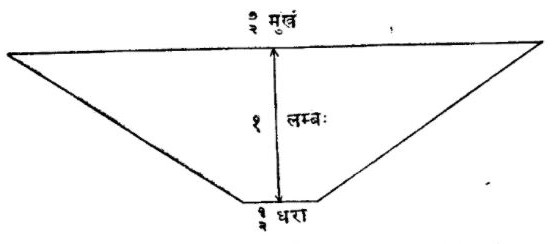
\includegraphics[width=8cm, height=4cm]{img1.JPG}

{अस्य हास्तिकक्षेत्रस्य क्षेत्रफलं\textendash \;भूमुखयोगः ४, अर्धं २, लम्बेन १
एतद्गुणितं तदेव २~।}
{प्रथमपदे उत्तराभावादादिरेव फलमिति~।}

\newpage

{पञ्चहास्तिकक्षेत्रकल्पना\renewcommand{\thefootnote}{\s १}\footnote{\s *क्षत्र*~।} यथा\textendash \,वदनं \begin{tabular}{|c|}७ \\ २\\ \hline\end{tabular}\,, धरया \begin{tabular}{|c|}१ \\ २\\ \hline\end{tabular}\,, ऊनं
३, इष्टावलम्बकेनानेन}
{५ गुणितं १५, भू\textendash \hspace{-3mm} \begin{tabular}{r}१\\
२ \end{tabular} \hspace{-5mm} \textendash \,युतं\renewcommand{\thefootnote}{\s २}\footnote{\s युतं ३१~।}\begin{tabular}{r}३१\\
२ \end{tabular}(मुखम्)~।}
\vspace{3mm}

न्यासः\textendash 

\hspace{15mm} \includegraphics[width=9.5cm, height=4cm]{Images/img2.JPG}

{भूमुखयोगः १६, अर्धं ८, लम्ब\textendash \,५\textendash \,हतम् ४०~।}
\vspace{3mm}

{अपरः प्रश्नः\textemdash}

\begin{quote}
\hspace{3cm} {\eg ऽर्धे च~।}
\end{quote}

{द्व्यादित्रिचयश्रेढ्याः\renewcommand{\thefootnote}{\s ३}\footnote{\s द्यादि त्रिचये*~।} किं गणितमर्धपदे~।}
\vspace{3mm}

{न्यासः\textendash \hspace{4mm} आ २, उ ३, पद \begin{tabular}{|c|}१\\ २\\ \hline \end{tabular}~।\renewcommand{\thefootnote}{\s ४}\footnote{\s आ २ उक्रपा
\begin{tabular}{|c|}१\\ २\\\hline \end{tabular}~।}}
\vspace{2mm}

{कर्म\textendash \,पदं\begin{tabular}{r}१ \\
२ \end{tabular}रूपेण १ हीनं विसदृशच्छेदत्वात् \hyperref[32.1]{'छेदनमच्छेदनस्य रूपं स्यात्'} इति रूपस्य}
{रूपे छेदे\renewcommand{\thefootnote}{\s ५}\footnote{\s रूपेच्छेदने~।} कृते \hyperref[36]{'तुल्येन भागजातौ छित्वा छेदेने'}त्यादिना छेदसादृश्ये
कर्मणि\renewcommand{\thefootnote}{\s ६}\footnote{\s कर्म~।} जातम् \begin{tabular}{|r} १\\ २\\\hline \end{tabular} \hspace{-5mm} \begin{tabular}{r|} २\\ २\\\hline \end{tabular}}
{अर्धात् द्वौ द्विच्छेदौ पातयितव्यावधिकत्वान्न पतत इति यावत्सम्भवमर्धम् एव
संशोध्यायराशौ}
{निःशेषिते व्ययराशिरर्धमवशिष्यते तच्च}
\vspace{2mm}

\hspace{2cm}{\qt 'स्याद्योगे\renewcommand{\thefootnote}{\s ७}\footnote{\s युयोग~।} वियदूनेभ्यो वियोगे तद्विपर्ययः'\renewcommand{\thefootnote}{\s ८}\footnote{\s वियोगस्त*~।}}
\vspace{3mm}

\noindent{इति धनात्मकं सद्विपर्ययादृणं जायते \begin{tabular}{|c|} $\begin{matrix}
\mbox{{१}}\\
\mbox{{२}}
\end{matrix}+$\\\hline \end{tabular} इयति कृते जातं व्येक इति,
तस्यार्धं
\begin{tabular}{|c|} $\begin{matrix}
\mbox{{१}}\\
\mbox{{४}}
\end{matrix}+$\\\hline \end{tabular}\,, चयेन}
{३ गुणितं \begin{tabular}{|c|} $\begin{matrix}
\mbox{{३}}\\
\mbox{{४}}
\end{matrix}+$\\\hline \end{tabular}\,, आदिः (२) एतेन युतमिति विसदृशच्छेदत्वात्\renewcommand{\thefootnote}{\s ९}\footnote{\s विशदृश*~।}
\hyperref[32.1]{'छेदनमच्छेदनस्य रूपं स्यात्'} इति रूपद्वयस्य\renewcommand{\thefootnote}{\s १०}\footnote{\s रूपेद्वय*~।} रूपे छेदने कृते \hyperref[36]{'तुल्येन भागजातौ छित्वे'}त्यादिना छेदसादृश्यकर्मणि}
{जातम् \begin{tabular}{|c|} $\begin{matrix}
\mbox{{३}}\\
\mbox{{४}}
\end{matrix}+$\\\hline \end{tabular}\begin{tabular}{r|} ८\\ ४\\\hline \end{tabular} अनयोर्योगे कार्ये {\qt 'तयोर्योगे वियोगः स्यात्'} इति ऋणस्य
धनात् विशुद्धौ}
{जायते \begin{tabular}{|c|} ५\\ ४\\\hline \end{tabular} इयता कृतेन\renewcommand{\thefootnote}{\s ११}\footnote{\s कृतं~।} जातं सादिः, पदेन\begin{tabular}{r}१ \\
२ \end{tabular}गुणितम्\begin{tabular}{r}५ \\
८ \end{tabular}, एतत्
गणितम्\renewcommand{\thefootnote}{\s १२}\footnote{\s गुणितं~।}\,।}

 \end{document}